

\date{\today}

\documentclass[12pt]{article}
\usepackage{subfig}
\usepackage{graphicx}
\usepackage{graphics}
\usepackage{longtable}
\usepackage{multirow}
\usepackage{color}
\usepackage{caption}
\usepackage{array}
\usepackage{hyperref}
\usepackage{tikz}
\usepackage{gnuplot-lua-tikz}
\usepackage{amssymb,amsfonts,amsmath,textcomp}
\usepackage{scalerel}
\usepackage[final]{listings}
\usepackage{color}
\usepackage{xcolor}
\usepackage{algorithm}
\usepackage{algpseudocode}


\definecolor{greyr}{RGB}{135,139,133}
\definecolor{greyb}{RGB}{80,80,100}
\definecolor{geditstring}{RGB}{255,22,255}
\definecolor{gedittype}{RGB}{49,139,87}
\definecolor{geditkeyword}{RGB}{167,40,44}
\definecolor{geditmacro}{RGB}{163,32,243}
\definecolor{cppruler}{RGB}{148,224,61}
\definecolor{pythonruler}{RGB}{106,204,209}
\definecolor{MFEMDarkGreen}{RGB}{0,100,0}
\definecolor{MFEMGreen}{RGB}{0,255,0}
\definecolor{MFEMForestGreen}{RGB}{34,139,34}
\newcommand{\f}[1]{FEniCSx#1}
\newcommand{\vm}[1]{
	{\ensuremath{\mathbf{#1}}}
}
\newcommand{\tens}[1]{
	{\ensuremath{\mathsf{#1}}}
}
\newcommand{\stretchint}[1]{
	{\vcenter{\hbox{\stretchto[440]{\displaystyle\int}{#1}}}}
}
\newcommand{\mycode}[1]{\textsf{"}\lstinline`#1`\textsf{"}}
\newcommand{\mycodepy}[1]{\textsf{"}\lstinline[language=Python]`#1`\textsf{"}}

\graphicspath{ {doc.data/img/} }

\lstset{
	language=[ISO]C++,
	breaklines=true,
	tabsize=2,
	showstringspaces=false,
	captionpos=b,
	numbers=left,
	caption={~},
	numberstyle=\tiny,
	basicstyle=\small,
	stringstyle=\color{geditstring},
	directivestyle={\color{geditmacro}},
	commentstyle=\color{blue},
	%identifierstyle=\color{greyr},
	deletekeywords=[1]{const,char,unsigned,int,short,double,float},
	morekeywords=[2]{const,char,unsigned,int,short,double,float},
	keywordstyle={[1]\color{geditkeyword}},
	keywordstyle={[2]\color{gedittype}},
	frame=shadowbox,
	rulesepcolor=\color{cppruler},
	rulecolor=\color{cppruler},
	escapechar={é}
}
\lstdefinelanguage{Python}
{
	morecomment=[l]{\#},
	morekeywords=[1]{import,from,def,return,lambda},
	morekeywords=[2]{list,map,str,eval},
	morekeywords=[3]{dolfinx,basix,ufl,classes,tensors,fem,mesh,la,nls,petsc},
	morekeywords=[4]{dx,Constant,Mesh,element,FunctionSpace,Coefficient,TrialFunction,TestFunction,FacetNormal,sqrt,grad,inner,tr,Identity,dot,ds,conditional,lt,gt,eq,derivative,diff,tensor,variable,as_tensor,create_element,functionspace,Function,NonlinearProblem,LinearProblem,NewtonSolver,form,apply_lifting,set_bc,assemble_vector,assemble_matrix,locate_entities,locate_dofs_topological,dirichletbc,interpolate},
	keywordstyle={[2]\color{green}},
	keywordstyle={[3]\color{orange}},
	keywordstyle={[4]\color{cyan}},
	rulesepcolor=\color{pythonruler},
	rulecolor=\color{pythonruler}
}
%\DeclareCaptionFormat{listing}{\rule{\dimexpr\textwidth+17pt\relax}{0.4pt}\par\vskip1pt#1#2#3}
%\captionsetup[lstlisting]{format=listing,singlelinecheck=false, margin=0pt, font={sf},labelsep=space,labelfont=bf}
\DeclareCaptionFormat{listing}{\tiny\raggedleft#1#2#3}
\captionsetup[lstlisting]{format=listing,singlelinecheck=false, margin=0pt, font={sf},labelsep=space,labelfont=it}


\title{\f{} and MFEM libraries comparison  }
%\author{	Alexis Salzman }

\begin{document}
\maketitle

\begin{abstract} 	
	This work provides a partial comparison of two   libraries:  \f{} and MFEM . The evaluation focuses on various aspects such as the problem encoding complexity, available documentation, computational performance, input/output (I/O) capabilities, support for parallelism, dependency constraints imposed by the various software tools used by these libraries,  .... By examining these factors, we aim to offer some insights into the strengths and weaknesses of each library,  enlightening researchers and engineers in selecting a  suitable tool for their specific computational needs. The analysis includes practical coding examples, performance benchmarks, and a detailed discussion on the ease of use and scalability, providing a partial assessment of each library's capabilities and usability. This document can also be used as a light tutorial to start encoding in one library knowing the other.
\end{abstract}
\section{Introduction}
\f{} and MFEM are both open-source libraries used for solving partial differential equations (PDEs) using finite element methods (FEM).
The target audience for this document is diverse: it ranges from newcomers to both codes ( but familiar with the principle of the finite element and with the formulation of a physical problem in weak form)  who are looking for insights to help them choose one or the other, to users who are tempted to switch from one to the other, to intermediate users who are looking at some details in one library with a view to possibly using the approach of the other library,...

Written  primarily  in Python with core components in C++, \f{}  focuses on providing a high-level, user-friendly interface to FEM. It is designed to be accessible to users with minimal programming experience, without compromising on computational performance and scalability.
It is part of the FEniCS project, with significant contributions from the scientific computing community.

MFEM is primarily written in C++ with interfaces for Python. It focuses on being a high-performance, scalable finite element discretization library. MFEM requires more familiarity with programming, particularly C++, for advanced use. It is developed by the Center for Applied Scientific Computing at Lawrence Livermore National Laboratory. 


As free libraries, they can be downloaded from  \url{https://fenicsproject.org/} for \f{}(version 0.8.0 in this work) and from  \url{https://mfem.org} for MFEM (version 4.7.0 in this work). Both offers a wide range of possibilities for solving various physical problems in a fairly general way.  To get an idea of how problems are formulated in each library, a series of examples will be used to compare them. In this work only parallel example will be used. These examples are structured so that the following topics, common to many simulations using FEM libraries, can be compared:
\begin{enumerate}
	\item Initialize the library\label{point_init}:
	\begin{itemize}
		\item Put in place MPI context.
		\item Parse command-line options.
	\end{itemize}
\item Mesh construction\label{point_mesh}: 
	\begin{itemize}
	\item Read or create the mesh.
	\item Distribute the mesh in parallel MPI context
	\item Eventually refine the mesh.
    \end{itemize}
\item Define a finite element space using the mesh and a given polynomial order. \label{point_space}

\item Define material properties:\label{point_mat}
\begin{itemize}
	\item Potentially different for some sub-domain.
	\item Not forcefully constant during the simulation.
\end{itemize}
\item Boundary Conditions and Load:\label{point_bc}
\begin{itemize}
	\item Define essential boundary conditions (Dirichlet)
	\item Set up the right-hand side or the residual (Neuman,...)
\end{itemize}
\item Linear or non-linear problem creation:\label{point_matrix}
\begin{itemize}
	\item Assemble various matrices and vectors.
	\item In non-linear set up initial solution.
\end{itemize}
\item Solve the system:\label{point_solve}
\begin{itemize}
	\item In general pass a linear system to an external library dedicated to solve this kind of system in parallel.
	\item In non-linear loop to update material properties and solve again the new linear system up to convergence (null residual)
\end{itemize}
\item Output:\label{point_out}
\begin{itemize}
	\item Save the different field in files that can be read by visualization tools
\end{itemize}
\end{enumerate}

The following section comments on each of these topics. The implementation of the examples in the  section \ref{example} is not fully provided in this document. 
Only parts of the code are used in support of the main explanations.
The full implementation can be found in the following repository:
\noindent \url{https://github.com/SalzmanA/fem-libraries.git}

\section{Examples\label{example}}
\subsection{Mechanic}
\subsubsection{Asymmetric traction/compression elasto-damaged constitutive law}\label{expl1}

This test case is designed to evaluate the behavior of a square sample (1mx1m) under traction or compression (Dirichlet boundary condition) and volume loading ($\vm{f}$)
, considering an elasto-damaged constitutive law that accounts for asymmetric traction/compression responses. The model employs a poly-crystalline structure generated by Neper library\cite{Neper,QUEY20111729}, introducing variability in material properties to mimic real-world conditions :

\begin{itemize}
	
\item Mesh Generation: The mesh for the square domain $\Omega$ is obtained using Neper and saved in  gmsh format(Figure \ref{mesh}).
\item Damage Field:  An arbitrary damage field is created, introducing total stiffness losses at certain grain interfaces (Figure \ref{damage}).
\item Grain Properties: Grains are modeled as isotropic materials, with no material orientation inside a grain.
\item Young's Modulus Variation: Each grain has a different Young's modulus, with random values in the range [5e6Pa, 1e8Pa] (Figure \ref{E_young}).
\end{itemize}
\begin{figure}
	\includegraphics[width=1.\textwidth]{neper.png}
	\caption{2D Mesh created by Neper (color represent different physical properties tag). \label{mesh}}
\end{figure}
\begin{figure}
	\centering
	\includegraphics[width=1.\textwidth]{dam.png}
	\includegraphics[width=0.7\textwidth]{dam_extrude.png}
	\caption{Imposed damage computed for a refined mesh, in MFEM (left top) \f{\_C++}(center top) and in \f{\_py}(right top). Bottom image presents  an elevation of the damage field (z=d) with value at nodes using a lateral view angle. It aims to shows the chosen arbitrary damage profile imposed around border of grain fixed to 1 . \label{damage}}
\end{figure}
\begin{figure}
	\includegraphics[width=1.\textwidth]{E.png}
	\caption{Grain Young's Modulus values in Pa after creation in MFEM (left), \f{\_C++}(center) and  \f{\_py}(right).\label{E_young}}
\end{figure}
Spatial discretization will use order 1 Lagrange polynomial. The constitutive law in 2D is based on the following potential:  
\begin{equation}
	\psi(\tens{\epsilon},d)=\frac{\lambda}{2}\left( 1-\alpha d\right)tr(\tens{\epsilon})^2 + \mu \sum_{i=1}^{2}(1-\alpha_i d){\Lambda_i}^2 
	\label{freeenergy}
\end{equation}
where:
\begin{itemize}
	\item $\lambda$ and $\mu$ are the Lam\'{e} elasticity coefficients.
	\item $\Lambda_i$ are the eigenvalues of the strain tensor $\tens{\epsilon}$.
	\item $ \alpha_i$ and $\alpha $ are coefficients introduced to take into account an asymmetric behavior in traction/compression:
	\begin{itemize}
		\item $ \alpha_i = 0 ~ if~ {\Lambda_i}<0$
		\item $ \alpha_i = 1 ~ if~ {\Lambda_i}\geqslant 0$
		\item $ \alpha = 0 ~ if~ tr(\tens{\epsilon})<0$
		\item $ \alpha = 1 ~ if~tr(\tens{\epsilon})\geqslant 0$
	\end{itemize}
\end{itemize}

The Cauchy stress tensor $\tens{\sigma}$ is  obtained from the free energy $\psi$ as follows:
\begin{equation}
		\tens{\sigma} = \frac{\partial\psi}{\partial\tens{\epsilon}}
		\label{sigfromphi}
\end{equation}  

The variationnal formulation to encode in the libraries considering non-linear behavior is thus the residual computation. If  $\mathcal{M}$ is the  continuous space of the problem defined on $\Omega$ and compatible with the Dirichlet boundary conditions ($\mathcal{M}_0$ being $\mathcal{M}$ with null Dirichlet boundary conditions) the residual is given by:

\begin{equation}
	F\left( \vm{u},\vm{v} \right)_{\Omega} =\stretchint{5ex}_{\Omega}
	\tens{\sigma \left( \vm{u} \right)}:\tens{\epsilon}\left( \vm{v}\right)\mathrm{d}V
	-\stretchint{5ex}_{\Omega} \vm{f}.\vm{v}\mathrm{d}V 
	\label{formF}
\end{equation}
with:
\begin{itemize}
	\item $\vm{u}\in \mathcal{M}$ is the displacement at current non-linear iteration
	\item $\vm{v}\in \mathcal{M}_0$ is the test function
	\item $\vm{f}$ is an arbitrary imposed Neumann load (in Newton), shown in the figure \ref{load} and given by the equation \eqref{load1}.
\end{itemize}

\begin{equation}
\vm{f}=\left\{ \begin{array}{l}
		-100000 (1600-(y-0.5)^2-500)*(x-0.5)^3\\
		0.
\end{array}\right.
\label{load1}
\end{equation}
\begin{figure}
	\includegraphics[width=1.\textwidth]{load.png}
	\caption{Arbitrary imposed interior loading interpolated on refined mesh by MFEM (left), \f{\_C++}(center) and by \f{\_py}(right). It is the X component value of the 2D vectorial forces $\vm{f}$ that is shown.\label{load}}
\end{figure}
The Jacobian matrix needed in the non-linear resolution is given by differentiating \eqref{formF}.

Finally, small strains and displacements are assumed which  implies the following strain tensor/displacement relation: 
\begin{equation}
	\tens{\epsilon}=\frac{1}{2}\left(\nabla\vm{u} +\left(\nabla \vm{u}\right)^t\right)~\text{on}~\Omega
	\label{eps}
\end{equation}
The first $i_1$ and the second $i_2$ invariant of $\tens{\epsilon}$ are given by the following formulas:
 \begin{equation}
 	\begin{array}{l}
 		i_1=tr(\tens{\epsilon})\\
 		i_2=\frac{1}{2}\left( tr(\tens{\epsilon}^2)- i_1^2 \right)
 	\end{array}\label{invariants} 
 \end{equation}

\section{API and documentation}

As already mentionned the \f{} language is primarily Python with core components in C++. 
In fact, the C++ sources are divided into the following libraries:
\begin{itemize}
	\item dolfinx: Problem solving environement
	\item basix: \f{} finite element basis evaluation library 
	\item ufl: UFL - Unified Form Language 
	\item ffcx: Form compiler for finite element forms 
\end{itemize}
The Python API follows this division and provides modules for each library. 
It also gives some extra features not (yet) available in C++ like gmshio.  


\bigskip
For MFEM it is the other way round, the language is primarily C++ with interfaces to Python.
The C++ sources are packaged in a monolithic library called MFEM, and the Python warping is provided by PyMFEM (has not yet been tested in this study).
The C++ API is encapsulated in the unique namespace \mycode{mfem}.
	
\bigskip
The table \ref{libstd} gives the requirements for C++ compilers and python interpreters, and the following setting is  used in this document for  \f{} C++ code:
\begin{table}
	\centering
	\begin{tabular}{|c|c|c|c|}
		\hline
		\multicolumn{2}{|c|}{\f{}}&\multicolumn{2}{c|}{MFEM}\\
		\hline
		C++&python&C++&python
		\\
		\hline
		C++20&\multirow{2}{*}{3.10}&\multirow{2}{*}{C++11}&\multirow{2}{*}{?}\\
		C++23 add-on&&&\\
		\hline
	\end{tabular}
	\caption{ Required standard/version to compile/run\label{libstd} }
\end{table}
 
\begin{lstlisting}[numbers=none,basicstyle=\scriptsize,label=typedeffenicsx]
	using namespace dolfinx;
	typedef PetscScalar scalar;
	typedef scalar_value_type_t<scalar> scalar_dolf;
\end{lstlisting}
and MFEM code:
\begin{lstlisting}[numbers=none,basicstyle=\scriptsize,label=typedefmfem]
	using namespace mfem;
\end{lstlisting}

	
In terms of documentation and community, \f{} has a strong forum (\url{https://fenicsproject.discourse.group}) inherited from the FEniCS project. 
All APIs are documented at \url{https://docs.fenicsproject.org}. 
An "official" tutorial is available at \url{https://jsdokken.com/dolfinx-tutorial/} and some interesting contributions can be found on "unofficial" sites such as J. Bleyer's (\url{https://bleyerj.github.io/comet-fenicsx/index.html}) or J.S. Doken's (\url{https://jsdokken.com/tutorials.html}).
From an external point of view, the \f{} project is (at the time of writing) in a state of intense development, so the material that can be found on the web can sometimes be a bit confusing (examples based on an old APi or related to FEniCS, site related to unofficial addons more or less up to date with the current version, thread in the forum obsolete due to library evolution, ....  ). 
But as development moves fast, so does documentation.

For its part, MFEM makes all the interesting material available on its website (\url{https://mfem.org}), with a discussion forum within the source github repository: \url{https://github.com/orgs/mfem/discussions}.

\bigskip
For both libraries, many examples provide a nice tutorial to get into the implementation of a problem. 
The API documentation provides the remaining ingredient to complete the encoding.
\section{Initialize (point \ref{point_init})}
In parallel, the minimum to implement is the initiation of the MPI library, and as FEnicsx and MFEM may use it, in addition, the initiation of PETSC. 
With \f{} C++ API,   a logging tool can also be set up at start-up, using the following code:
\begin{lstlisting}[numbers=none,basicstyle=\scriptsize]
// Init logging backend of dolfinx (loguru)
// tuned by -dolfinx_loglevel <level> option
dolfinx::init_logging(argc, argv);
// init petsc environment
// imply init distributed environement
PetscInitialize(&argc, &argv, nullptr, nullptr);
std::string log_name = "what you want distinquishing PID";
loguru::set_thread_name(log_name.c_str());
// very verbose
loguru::g_stderr_verbosity =loguru::Verbosity_INFO;
// only warning
loguru::g_stderr_verbosity =loguru::Verbosity_WARNING;
\end{lstlisting}
With the version used in this study (0.8), \f{} uses the logger library loguru. 
But they switched to the spdlog library in the next release.
Here using \mycode{PetscInitialize} function (and \mycode{PetscFinalize} at the end of the program) make Petsc library call the \mycode{MPI_init} function. 
If Petsc is not to be used,  \mycode{MPI_init} (or \mycode{MPI_Init_thread}) must be called directly (and \mycode{MPI_finalize} at the end of the program). 

The python conterpart corespond to the importation of all used module as  follow:
\begin{lstlisting}[numbers=none,basicstyle=\footnotesize,language=Python]
	from scipy import sparse
	from mpi4py import MPI
	import numpy as np
	from pathlib import Path
	from ctypes import CDLL
	import sympy as sp
	import ufl
	from ufl.classes import (Mesh,FunctionSpace,Coefficient,Constant,
	TrialFunction,TestFunction,FacetNormal)
	from ufl import ( sqrt,grad,inner,tr,Identity,dot,dx,ds,
	conditional,lt,gt,eq)
	import basix	
	from dolfinx.io import XDMFFile
	from dolfinx.io import VTXWriter
	from dolfinx import fem
	from dolfinx import mesh
	from dolfinx import la
	from dolfinx import nls
	from dolfinx import cpp
	from dolfinx.fem import petsc
	from dolfinx.nls import petsc
	import adios4dolfinx
	from petsc4py import PETSc
\end{lstlisting}

MFEM does not seem to rely on a  logger library strategy. Information is output to a stream on demand, using a special printing method or setting a log level with some algorithms. Or, at compile time, the MFEM\_DEBUG macro, if set, forces messages to be output from any routine that encodes them.
Compared to \f{}, the \mycode{MPI_init} function must be called in MFEM code using its \mycode{mfem::Mpi} class, which encapsulates the MPI library, with the \mycode{mfem::Mpi::Init} method (and the \mycode{mfem::Mpi::Finalize} at the end of the program).
MFEM provides a handy options parser, unlike \f{}, which allows you to encode options in the source and modify them at runtime with the parameters passed to the program at startup.
In the following code, for example, \mycode{newton_rel_tol} is set to 1.e-7 in the source and can be changed at runtime using the \mycode{-rel} or \mycode{--relative-tolerance} option:
\begin{lstlisting}[numbers=none,basicstyle=\scriptsize]
Mpi::Init(argc, argv);
const char *petscrc_file = "";
OptionsParser args(argc, argv);
args.AddOption(&petscrc_file, "-petscopts", "--petscopts", "PetscOptions file to use.");
args.AddOption(&verbose, "-v", "--verbose", "-nv", "--not-verbose", "Output extra informations.");
real_t newton_rel_tol = 1e-7;
real_t newton_abs_tol = 5e-8;
args.AddOption(&newton_rel_tol, "-rel", "--relative-tolerance", "Relative tolerance for the Newton solve.");
args.AddOption(&newton_abs_tol, "-abs", "--absolute-tolerance", "Absolute tolerance for the Newton solve.");
args.Parse();
if (!args.Good()){
   	if (mpi_rank == 0)  args.PrintUsage(cout);
   	return 1;
   }
if (mpi_rank == 0)  args.PrintOptions(cout);
   
\end{lstlisting}
To use Petsc in MFEM, the program must call \mycode{MFEMInitializePetsc} (and \mycode{MFEMFinalizePetsc} at the end):
\begin{lstlisting}[numbers=none,basicstyle=\scriptsize]
MFEMInitializePetsc(NULL, NULL, petscrc_file, NULL);   
\end{lstlisting}
Here a \mycode{petscrc_file} file can be provided at runtime to tune Petsc.

\section{Mesh(point \ref{point_mesh})\label{Mesh}}
\subsection{Reading\label{Mesh_reading}}
In most example, MFEM use the following strategy that start from a serial mesh defined in a file:
\begin{itemize}
	\item Read the file in all process (via \mycode{mfem::Mesh} constructor) and create a serial  instance of the full mesh. This implies that the mesh is relatively coarse to fit in memory on all processes.
		\item Create a parallel mesh instance (\mycode{mfem::ParMesh}) in all process using the serial mesh instance and a partition provided by the user or, by default, computed by METIS (from the full serial mesh dual-graph). After construction, on each process, this parallel mesh only contains the part of the serial mesh related to the partition with the  rank id of the process.
		\item Refine the coarse distributed mesh.
\end{itemize}






The above scheme works with MFEM (conforming, non conforming, nurbs), Netgen, TrueGrid, VTK, GMSH, NETCDF, Cubit file format.

One constructor of \mycode{mfem::ParMesh} class accepts also a stream argument that give the ability to read a parallel mesh with each MPI rank using its own file/stream. It has not been tested but from source file investigation it looks like it works only with parallel MFEM mesh format (i.e. with a set of file/stream with each having specific information related to mesh distribution). 

With C++ API, \f{} can use XDMF reader (\mycode{dolfinx::io::XDMFFile::read_mesh}) to load mesh into \mycode{dolfinx::mesh::Mesh<T>} instance. Compare to MFEM above strategy this method can, if XDMF file use HDF5 storage format, read on each process only a part of the serial mesh stored in this file.
The mesh is then redistributed using the partition created in parallel by the user or by ParMetis (or PtScotch or Kahip).
With this method, if the starting mesh is very fine, there can be no memory problem because a process only holds a portion of the mesh during the entire read.
 The drawback is that the amount of communication is higher compared to the MFEM strategy, where all processes perform the same serial computation without exchanging information.
 This can be seen in figures \ref{time_mesh} and \ref{time_mesh_r} with test case of section \ref{expl1}. The MFEM curve related to mesh reading is almost constant as all process do the same amount of work (reading,partitioning,filtering). In comparison, \f{} scale up to 8 processes and its reading performance stagnate or decrease with 16 process and above (parmetis is certainly using to much process for the given mesh dual-graph size, hardware i/o may be saturated and redistribution may involve too much communication)   
 
 At the time of writing, the \f{} C++ API does not provide any other mesh reader for any other mesh format.
 Only the Python API provides, in addition to XDMF,  interaction with Gmsh by directly translating a Python gmsh API mesh model into a Dolfinx mesh via gmshio.
 By the way, it is this gmshio module that has been used to generate XDMF files from gmsh Neper files for the test case of the section \ref{expl1}:

 \begin{lstlisting}[numbers=none,basicstyle=\footnotesize,language=Python]
 from mpi4py import MPI
 from dolfinx.io import XDMFFile, gmshio
 msh, c, e = gmshio.read_from_msh("path/to/gmsh/file", MPI.COMM_WORLD, gdim=2)
 # arbitrary name
 msh.name = "neper_dam" 
 c.name = f"{msh.name}_cells"
 e.name = f"{msh.name}_facets"
 with XDMFFile(msh.comm, "path/to/xdmf/file", "w") as file:
 	file.write_mesh(msh)
 	file.write_meshtags(c, msh.geometry, geometry_xpath=f"/Xdmf/Domain/Grid[@Name='{msh.name}']/Geometry")
 	file.write_meshtags(e, msh.geometry, geometry_xpath=f"/Xdmf/Domain/Grid[@Name='{msh.name}']/Geometry")
\end{lstlisting}
 
 
 With the Python API, reading the xdmf file gives the same kind of performance as with the C++ API, as can be seen in figures \ref{time_mesh} and \ref{time_mesh_r} (variation are certainly due to I/O hardware).
 
 
 \begin{figure}
 	\includegraphics[width=1.\textwidth]{part.png}
 	\caption{Mesh distribution on 64 processes by MFEM (left) \f{\_C++}(center) and \f{\_py}(right) of the test case of section \ref{expl1}.\label{Partition}}
 \end{figure}
  
\subsection{Partitioning\label{partitioning}} 
 In figure \ref{Partition} the mesh distribution of the test case of section \ref{expl1} for both library is shown for 64 processes. 
 The partitioning is naturally\footnote{See paper on ParMetis/Metis} not the same as MFEM use Metis on full serial mesh dual-graph, and \f{}, Parmetis on an arbitrary distributed mesh dual-graph. In both case the nested dissection algorithm  roughly divided the full square mesh in four blocks themselves divided in four sub blocks and so on. It appears more clearly with MFEM/Metis where pids are following the dissection and no inital mesh distribution interferes in the process of partionning.
 
 
 The term "ghost" used in MFEM and \f{} when using distributed meshes means that some entities are duplicated between processes to achieve certain objectives.
 At the very least, all entities at the boundary between different processes are duplicated in all those processes (i.e. in 1D nodes, in 2D nodes and edges and in 3D nodes, edges and faces). This ensures that the elements connected to the boundaries of a process have the correct geometric and topological definition. 
 
 Otherwise, cells can be duplicated in all connected processes for specific calculations.
 With \f{} it's when  reading a mesh that the \mycode{dolfinx::mesh::GhostMode} can be selected. It can be:
 \begin{itemize}
 	\item none: There is no cell duplication
 	\item shared\_facet:   For an edge (2D) or face (3D) inside the part but at the boundary of 2 processes, all its related cells are present in both processes.
 	\item shared\_vertex: Apparently, at the time of writing, this is equivalent to shared\_facet for 2D/3D mesh. It may be related to 1D meshes that have not yet been tested. 
 \end{itemize}
 \begin{figure}
	\centering
	\includegraphics[width=0.8\textwidth]{ghost.png}
	\caption{\f{} ghosting illustration with a mesh distributed over 2 processes. On the left, the mesh distributed on 2 processes without ghost cell (one colour for each process). On the right, cells present on one process with (bottom) and without (top) ghost cells. \label{ghost}}
\end{figure}
Figure \ref{ghost} illustrates the ghost modes of \f{} with a simple 2D mesh distributed over 2 processes.
 

MFEM does not have ghost cells in its mesh structure. Only references to neighbours in other processes are created and communication occurs when data needs to be used for computation.

In any case, to keep the numbering (mesh/dof) consistent, a notion of "owner" is introduced for ghost entities. Among all processes holding an instance of an entity, one is arbitrarily chosen to "own" that entity. Numbering is thus imposed by "owner" processes, and other processes inherit this numbering. For example, in both libraries, vertices are owned by the process with the smallest process ID.

\subsection{Refining} 
 
Both libraries provide a refinement strategy (local or global). MFEM is more general in this aspect as it can generate non-conforming mesh (with control of hanging entities) and is able to derefine refined zone based on some error criteria.
This generality is made possible by a dedicated mesh database that stores the history of the refinement. In contrast, FEniCS's refinement tools generate a new mesh instance (or a set of information describing a mesh) and optionally the parent cell/face indices of child cells/faces.  
 
Only uniform refinement has been tested in this study.
The \mycode{UniformRefinement} method of the class \mycode{mfem::Mesh} of MFEM uses a simple algorithm to split cells:
\begin{itemize}
	\item generate a new vertex at the center of each edge
	\item based on the original vertex and the new middle vertices, generate sub-element: 2 in 1D, 4 in 2D, 8 in 3D (for pure tetrahedral meshes, an "A" or "B" algorithm with different quality control is proposed). 
\end{itemize}

\f{} with \mycode{dolfinx::refinement::plaza::refine} function use a more sophisticated algorithm related to the article \cite{PLAZA2000195}. In the 2D example of section \ref{expl1}
they provide almost the same refined mesh except that some element have been flipped (certainly to respect some mesh quality criteria) by \f{}(figure \ref{element_swap}).
 \begin{figure}
	\centering
	\includegraphics[width=0.8\textwidth]{ref2_mesh_difference.png}
	\caption{MFEM(red) and \f{}(blue) refined mesh of the test case of section \ref{expl1}. Both have the same number of nodes. MFEM follows always the same refinement pattern. In contrast, \f{} has spited some parallelipiped in a different way resulting on edges not parallel to any edges of the original refined element(center left elements in the view)).  \label{element_swap}}
\end{figure}
\subsection{Creating}
Regarding mesh creation on the fly, \f{} propose 1D (\mycode{create\_interval})/2D (\mycode{create\_rectangle})/3D (\mycode{create\_box}) interval, rectangle or box creation for quick testing. MFEM proposes \mycode{Mesh::MakeCartesian1D}, \mycode{Mesh::MakeCartesian2D} and \mycode{Mesh::MakeCartesian3D} for the same purpose.
And in both libraries, the mesh class API provides a way to code the creation of a mesh from scratch.
 

\section{Space and field(point \ref{point_space})\label{spaceField}}
With a mesh in hand, the creation of a finite element discretisation of a domain requires the definition of the finite element type.
\subsection{Finite element}
MFEM provides a large collection of finite elements of arbitrary order. They are grouped by family type represented by class that are all deriving from \mycode{mfem::FiniteElementCollection}. In 1D, 2D and 3D, families are (not exhaustive):
\begin{itemize}
	\item \mycode{mfem::H1\_FECollection}: Arbitrary order H$^1$-conforming (continuous) finite elements. 
	\item \mycode{mfem::L2\_FECollection}: Arbitrary order "L2-conforming" discontinuous finite elements.
	\item \mycode{mfem::ND\_FECollection}: Arbitrary order H(curl)-conforming Nedelec finite elements.
	\item \mycode{mfem::RT\_FECollection}: Arbitrary order H(div)-conforming Raviart-Thomas finite elements.
	\item ...
\end{itemize}
All these elements use a polynomial bases chosen at construction time. Note that not all elements can use all bases types. Selection is done using enumeration  of \mycode{mfem::BasisType} class: GaussLegendre, GaussLobatto(Lagrange), Serendipity, Positive (Bernstein), ...

The following code creates a finite element collection (called \mycode{fec}) representing an H$^1$-conforming element of dimension 2 and order 1 using (default argument) Gauss-Lobatto polynomial bases:\begin{lstlisting}[numbers=none,basicstyle=\footnotesize,label=feca]
H1_FECollection fec(1, 2);
\end{lstlisting}
For order 1 elements that are not intended to be extended to a higher degree in the application, it is cheaper to use a handmade simple linear base as encoded in the linear collection:\begin{lstlisting}[numbers=none,basicstyle=\footnotesize,label=fec]
LinearFECollection fec;
\end{lstlisting}
This is illustrated by the performance analysis in section \ref{perfass}.

In \f{} finite elements are related to the basix library. This library provides the class \mycode{basix::FiniteElement} which can hold any type of finite element. This class play the role of \mycode{mfem::FiniteElementCollection} but rely on generic structure to define finite elements compared to MFEM which use derivation for genericity. For a full list of basix built-in elements, see for example https://defelement.com/lists/implementations/. The type of element is chosen at instantiation time by calling the  \mycode{create\_element} function with the following arguments:
\begin{itemize}
	\item family: \begin{itemize}
		\item arbitrary order Lagrange-like: P or "Lagrange","DP","DG","DQ" or "P" string in python
		\item arbitrary order H(div)-conforming Raviart-Thomas: RT or "Raviart-Thomas", "N1F", "N1div", "Nedelec 1st kind H(div)", "RTCF", "NCF" or "RT" string in python
		\item arbitrary order H(curl)-conforming Nedelec: N1E or "N1curl", "Nedelec 1st kind H(curl)", "RTCE", "NCE" or "N1E" string in python
		\item ...
	\end{itemize}
	\item CellType; type of element (point, interval, triangle, tetrahedron,
	quadrilateral, hexahedron, prism or pyramid)
	\item degree: arbitrary order to use
	\item lagrange\_variant: specify the polynomial bases to be used and the DOF placement:
	\begin{itemize}
		\item unset: Use a default for each family, which depend on many aspects.
		\item equispaced: equi distance placement
		\item legendre: Legendre instead of Lagrange polynomial
		\item bernstein: Bernstein instead of Lagrange polynomial
		\item ...
	\end{itemize}All variants do not work with all element types. 
	\item discontinuous: If True element is discontinuous. The discontinuous element will have the same DOFs as a continuous element, but the DOFs will all be associated with the interior of the cell. 
\end{itemize}
With C++ API you can also call directly the function that creates an element related to a specific family (\mycode{basix::element::create\_lagrange} for P family,...). 

But in  \f{} there is no need to instantiate the basix element as in fact all the problem is defined has UFL expression (see \ref{Fenicx_form}). So in Python the function \mycodepy{basix.ufl.element} can be used instead of \mycodepy{basix.create_element} to create a UFL compatible element. It use the same set of parameter as \mycodepy{basix.create_element}. The following code creates a triangular finite element (called \mycodepy{elem}) using Lagrange polynomial bases of order 1 to interpolate 2-dimensional vector field on the element:\begin{lstlisting}[numbers=none,basicstyle=\footnotesize,language=Python,label=elem]
	elem = basix.ufl.element("Lagrange","triangle",1,shape=(2, ))
\end{lstlisting}
With the C++ API, the above code is placed in the Python script interpreted by ffcx (see section \ref{Fenicx_form}).

\subsection{Space} 
With the mesh and after instantiating an element (or a collection) of a given type, it is possible to create the finite element space on the domain.
 
In MFEM, with the finite element collection declared in listing \ref{feca} or \ref{fec} and a \mycode{mfem::ParMesh} pmesh (see section \ref{Mesh}), the space to interpolate a 2-dimensional vector field is created by the following instruction:
\begin{lstlisting}[numbers=none,basicstyle=\footnotesize,label=spacec]
ParFiniteElementSpace space(pmesh, &fec, 2, Ordering::byVDIM);
\end{lstlisting}
The \mycode{Ordering::byVDIM} value means that dofs are stored in an element by first looping over the  vector dimension (inner loop), then over the nodes (outer loop).
Alternatively, the user can select \mycode{Ordering::byNODES}, which loops first over the
 nodes (inner loop) and then over the vector dimension (outer loop).



With \f{}, using the Python API, the code to create a finite element space on the mesh given by \mycodepy{domain} with finite element \mycodepy{elem} declared in listing \ref{elem}, is:
\begin{lstlisting}[numbers=none,basicstyle=\footnotesize,language=Python]
space = dolfinx.fem.functionspace(domain, elem)
\end{lstlisting}
With the C++ API, the above code is placed in the Python script interpreted by ffcx and the space is retrieved as presented in  section \ref{Fenicx_form} listing \ref{generalfenicsxform}.  

\subsection{Field}
In MFEM, in parallel, a field can be created as an instance of the class \mycode{ParGridFunction}. An \mycode{x} field is created as follows, using the space defined in the previous section (listing \ref{spacec}):
\begin{lstlisting}[numbers=none,basicstyle=\footnotesize,label=xfield]
	ParGridFunction x(space);
\end{lstlisting}

With \f{}, the same field would be constructed in Python as follows
\begin{lstlisting}[numbers=none,basicstyle=\footnotesize,language=Python,label=pyx]
x=dolfinx.fem.Function(space,name='myfield')
\end{lstlisting}
And using the C++ API, considering that \mycode{V} is the space \mycodepy{space} collected from the Python script via ffcx (see for example listing \ref{generalfenicsxform}), the code is:
\begin{lstlisting}[numbers=none,basicstyle=\footnotesize,label=fieldfenics]
auto x = std::make_shared<fem::Function<scalar>>(V);
x->name="myfield"
\end{lstlisting}
where use of shared pointer to encapsulate the field object is related to coefficients argument of \mycode{dolfinx::fem::create\_form} function (see section \ref{Fenicx_form}). In this example in Python and C++, the field name is set to a dummy value \mycode{myfield}.
This is the name that will be attached to the field in the output files and will therefore be visible when the data is processed with Paraview or Visite or .....
\section{Material property(point \ref{point_mat})\label{MatProp}}
In the example in section \ref{expl1}, both libraries use cell tags to assign material to mesh elements. 
These tags come from the original Gmsh mesh files generated by Neper (figure \ref{mesh}).

With MFEM, Gmsh physical property are directly assigned to element attribute while reading mesh file. 
The element attribute is a single integer that can be accessed using the \mycode{GetAttribute} method of the \mycode{mfem::Element} class.
By default, no other data can be associated with elements.

In \f{}, tags are information that can be anything. They are stored outside the mesh/entities object in a dedicated template class (\mycode{template<typename T> dolfinx::mesh::MeshTags<T>}).
Therefore, when using gmshio, the Gmsh physical property must be transferred to the XDMF file in a separate location in the file tree structure(see section \ref{Mesh_reading}).
And when reading the XDMF file, either from C++ or Python API, extra instructions are mandatory to read the \mycode{mesh::MeshTags} objects. For these objects, the tag values are obtained using the \mycode{values} method.

These tags (integers) are then used with both libraries to set Young's modulus (and consequently Lamè coefficients $\lambda$ and $\mu$) using following expression:
\begin{equation}
	E(tag)=\frac{1.e^{8}-5.e^6}{199.}\times kr(tag)+5.e^6
\label{etag}
\end{equation}
with $kr()$ a semi-random function of tag (based on rand function of stdlib) that return an integer between 0 and 199.

For MFEM, the strategy adopted is to use a piecewise constant coefficient (\mycode{mfem::PWConstCoefficient}) directly for $\lambda$ and $\mu$. 
This \mycode{mfem::PWConstCoefficient} class uses constants keyed from the element attribute numbers. 
The \mycode{mfem::Vector} used to construct these objects are filled for each tag with the expressions of the Lamè coefficients as a function of Young's modulus given by \eqref{etag} and a constant Poisson's ratio value.

For \f{}, the choice has been made to start from Young's modulus (E) and Poisson's ratio($\nu$) in the construction of the formulation as shown in \ref{Fenicx_form}. In this case, E is a \mycode{dolfinx::fem::Function} initialised with \eqref{etag} and $\nu$ is a \mycode{dolfinx::fem::Constant}.
Perhaps starting from Lamè coefficients, as in MFEM, would be more computationally efficient, as the coefficient calculation would be skipped. But as the final formulation is itself written in C code, it's not obvious that we'll get any gain. Furthermore, replacing calls to  \mycode{dolfinx::fem::Function} and \mycode{dolfinx::fem::Constant} with two calls to  \mycode{dolfinx::fem::Function} may not be better.  (to be tested).  

\subsection{Damage\label{mat_dam}}
In the example in section \ref{expl1}, the material behaviour depends on a damage field. This field is constant throughout the simulation, but is calculated at the start based on an arbitrary setting of 1 at some grain boundary. The smoothing process, which produces the damage profile shown in figure \ref{damage}, is good for testing in parallel the interaction with the mesh database and field object of both libraries. The smoothing algorithm is very crude. It is presented in algorithm \ref{algo_dam}.
\begin{algorithm}[h]
\footnotesize
\begin{algorithmic}
	\State Create v\_dam\_cur and v\_dam\_new vectors to hold damage at nodes/dofs%\Comment{~}
	\State Set damage to 1 in v\_dam\_cur at some grain boundary nodes
	\For{iter\_smooth $\in[0,max\_smooth]$}
	\State v\_dam\_new$\gets 0$
	\For{ $i \in \mathfrak{L}$}
	\If{v\_dam\_cur$[i]<0.01$}
	\State v\_dam\_new$[i]\gets \displaystyle\sum_{k\in \mathfrak{N}_i}\text{v\_dam\_cur}[k]$
	\State Update ghost nodes v\_dam\_new values \Comment{~}
	\State v\_dam\_new$[i]\gets \max \left( \text{v\_dam\_cur}[i],\frac{\text{v\_dam\_new}[i]}{card\left(\mathfrak{N}_i\right)} \right)$
	\EndIf
	\EndFor
	\State v\_dam\_cur$\gets$v\_dam\_new
		\For{ $i \in \mathfrak{L}$}
	\State v\_dam\_new$[i]\gets \displaystyle\sum_{k\in \mathfrak{N}_i}\text{v\_dam\_cur}[k]$
	\State Update ghost nodes v\_dam\_new values \Comment{~}
	\State v\_dam\_new$[i]\gets \max \left( \text{v\_dam\_cur}[i],\frac{\text{v\_dam\_new}[i]}{card\left(\mathfrak{N}_i\right)} \right)$
	\EndFor
	\State v\_dam\_cur$\gets$v\_dam\_new
	
	\EndFor
\end{algorithmic}
\caption{Rough damage smoothing algorithm. $\mathfrak{L}$ is the set of node indices local to a process. $\mathfrak{N}_i$ is the set of nodes whose index is local to a process and connected to node $i$ by an owned edge. Inside the general loop, the first loop at node enlarges the non-zero damage zone and the second loop smooths and enlarges all non-zero damage zones. The general loop is just a repetition ( times) of the 2 loops on nodes. At the end, v\_dam\_cur contains the smoothed field. The $\triangleright$ icon indicates a communication step.\label{algo_dam}}
\end{algorithm}
It is mainly a loop to repeat an averaging process on all nodes using their topological neighbourhood. This averaging process is performed twice per loop. Once to enlarge the non-zero damage zones, examining only nodes with damage below a certain arbitrary threshold (0.01). Twice to average all the nodes and thus smooth the damage zone.
The averaging process required some communication as the topological neighbourhood of a node can be scattered in different domains/processes.

This algorithm has been used in MFEM and \f{} C++ implementations. In both cases, the underlying data array of the \mycode{d} field object was used directly (thanks to the order 1 Lagrange simplicity) to speed up the computation. In MFEM this was done by providing the underlying data array at construction time (avoiding costly use of \mycode{mfem::GridFunction::GetNodalValues} for example). And in \f{} it was done by calling \mycode{d->x()->mutable_array()} method, which directly gives a reference to the underlying data array.
The performance shown in figure \ref{time_dam} and \ref{time_dam_r} shows that both implementations scale relatively well despite the presence of the test that introduces imbalance.
Both library provides method to theire field class that easely scatter/gather information at ghost nodes.
MFEM is 2 to 6 times slower than \f{} C++, but has an additional speed-up rate.
This is certainly related to the use of roughly $max\_smooth \times \displaystyle\sum_{i\in \mathfrak{L}} card\left(\mathfrak{N}_i\right)$ operations. Depending on the threshold (0.01), this number can be augmented. In any case, when the domain is split in 2, $card\left(\mathfrak{L}\right)$ is roughly divided by 2, but also $card\left(\mathfrak{N}_i\right)$, for nodes on the process boundary,	 are reduced by some proportion. As the number of processes increases, the proportion of nodes at the domain boundary increases and the reduction in operation increases. But surprisingly, with the \f{} C++ implementation, this effect does not exist.

Regarding the \f{} Python implementation, if algorithm \ref{algo_dam} is implemented as loops like in the C++ implementation, the performance is of course catastrophic. 
In this study, after some testing, the two loops on the nodes were replaced by applying an operator to the field via a SciPy sparse matrix. Only loops on the topology remain to construct this operator. 
This is done once, but still costs a lot. Optimising this part, if possible,  would require some additional effort not related to this study. 
Therefore, the performance of the python implementation shown in figures \ref{time_dam} and \ref{time_dam_r} is poor (7 to 22 times slower) compared to other implementations in C++. This illustrates the fact that using the Python API requires care, so any algorithm not provided or constructable with \f{} must either be very well implemented or moved to a C/C++/Fortran implementation and encapsulated in a Python module.

The introduction of this damage locally, at some grain boundaries, theoretically results in unbalanced parallel domains, as we have not considered the additional cost of damage treatment during partitioning. In figure \ref{imbalence} on the left view, it appears that of the 128 processes, only 20 processes are traversed by a non-zero damaged zone.
\begin{figure}
	\includegraphics[width=1.\textwidth]{imbalance.png}
	\caption{Imbalence illustration with 128 cores (MFEM distribution). The left view is the superposition of the two right views, one of which is partially transparent. Only 20 processes is affected by the damage calculation.\label{imbalence}}
\end{figure}
As the damage zone is rather narrow, only a small proportion of the element in these 20 processes is affected by the damage calculation. This may explain why no major imbalance effect was observed in relation to the creation or effect of damage (see CV in table \ref{elapse}).
\begin{table}\footnotesize 
	\begin{tabular}{|c|l|c|c|c|c|c|}
		\cline{2-7}
		\multicolumn{1}{c|}{} & Task & val min & val max &CV& val avg & \% total avg \\ \hline
		\multirow{4}{*}{\rotatebox{90}{ MFEM}}      &  All & 8.578603 & 8.633553& 0.196100 & 8.608193 & 100.0 \\ \cline{2-7} 
		&  Define damage & 0.073467 & 0.074400 &0.002707& 0.073950 & 0.9 \\  \cline{2-7} 
		&  Elementary vector & 0.130437   & 0.164723  & 0.055433 &      0.134700 &          1.6 \\ \cline{2-7} 
		&  Elementary matrix & 0.078890  &  0.105820 & 0.067967& 0.083190 & 1. \\ \hline
		\multirow{4}{*}{\rotatebox{90}{\f{}}}      & All  & 13.518510 &     13.520770 &     0.004013 &     13.519100  & 100.0 \\ \cline{2-7} 
		&  Define damage & 0.042953&     0.043807&   0.001817 & 0.043407 &         0.3  \\ \cline{2-7} 
		&  Elementary vector & 0.046653 &      0.053423       &     0.006133 &      0.049870 &          0.4\\ \cline{2-7} 
		&  Elementary matrix & 0.078733 &     0.088870 &      0.011107 &      0.081627 &          0.6 \\\hline
	\end{tabular}
\caption{Elapsed times in seconds of some tasks related to damage for a simulation  with 128 processes (intermediate implementation)."val min" and "val max" are respectively the minimum and maximum computing time among all processes for the execution of the task."val avg" is the mean execution time of all processes to complete the task. The "CV" (100 $\times$"standard deviation"/"val avg"), representing the imbalance, is the coefficient of variation  multiplied by 100  to mimic a percentage of variation compare to mean value. "\% total avg" represent percentage of "val avg" of a task compare to "All"\label{elapse}}
\end{table}
Some calculations, not presented here, confirm (see CV in  table \ref{elapse_large}) that imbalance appears when the thickness of the damage band is increased (larger $max\_smooth$ in algorithm \ref{algo_dam}) and thus the proportion of elements with damage for these 20 processes is increased.
\begin{table}\footnotesize 
	\begin{tabular}{|c|l|c|c|c|c|c|}
		\cline{2-7}
		\multicolumn{1}{c|}{} & Task & val min & val max &CV& val avg & \% total avg \\ \hline
		\multirow{4}{*}{\rotatebox{90}{ MFEM}}      &  All & 12.22343 & 12.26745& 0.10736 & 12.24595 & 100.0 \\ \cline{2-7} 
		&  Define damage & 0.94938 & 0.95046 &0.00204& 0.94988 & 7.8 \\  \cline{2-7} 
		&  Elementary vector & 0.17121   & 0.22073  & 0.09661 &      0.19193 &          1.6 \\ \cline{2-7} 
		&  Elementary matrix & 0.10981  &  0.16517 & 0.16370& 0.14177 & 1.2 \\ \hline
	\end{tabular}
	\caption{Same type of result as in table \ref{elapse} for a larger damage band thickness simulation not shown in this study, which converges in 2 more non-linear iterations.\label{elapse_large}}
\end{table}
  
In any case, when distributing the mesh, both libraries allow the user to select a domain partition that can take damage costs into account if needed.
\section{System creation(point \ref{point_matrix})\label{systemcreation}}
System creation is related to variational expression of the problem. From finite element discretizations of variational forms, elementary vectors and matrices are computed and assemble into final system.
The approaches to compute finite element discretizations of variational forms (like \eqref{formF}) range from purely formal descriptions, which are close to mathematical expressions, to purely C++ programming implementations.

\subsection{\f{} variational expression \label{Fenicx_form}}
\subsubsection{General overview\label{gen_over}}
\f{} uses a formal description with a Unified Form Language (UFL). This description, provided by a Python script, is transformed into a C language code by the ffcx compiler. This code provides functions that transcript in elementary C instructions  the different form(s) and space(s) defined in Python script. Form functions, called "kernels",  are called by the assembly routine to obtain the elementary vector or matrix for a given finite element. When using full Python API this process is completely hidden to users that do not care to generate and branch kernels. With the C++ API, the user must branch the kernel compiled by ffcx using the following instruction, which illustrates the case of a linear and a bi-linear form defined on the same finite element space, on the full domain $\Omega$, using some coefficients and constants in the formulation:
\begin{lstlisting}[numbers=none,basicstyle=\scriptsize,label=generalfenicsxform]
// create function space object from python field "u"
auto V = std::make_shared<fem::FunctionSpace<scalar_dolf>>(fem::create_functionspace(SPACE, "u", pmesh));
// create linear form object
auto lin_form = std::make_shared<fem::Form<scalar, scalar_dolf>>(fem::create_form<scalar>(*FORM_L, {V}, coefficients,constants, {}));
// create bi-linear form object
auto bilin_form = std::make_shared<fem::Form<scalar, scalar_dolf>>(fem::create_form<scalar>(*FORM_BL, {V,V}, coefficients, constants, {}));
\end{lstlisting}
where:
\begin{itemize}
	\item \mycode{pmesh} pointer (shared) pointing to Mesh object discretizing $\Omega$ domain.
	\item \mycode{SPACE} is the name of the helper function generated by ffcx. It is used to create function space using function field name (i.e. name of the Python variable, here "u"). This function name starts with \mycode{functionspace_form_} followed by the name of the python script, followed by \mycode{_}, followed by the Python variable name of the considered form.
	\item \mycode{FORM_L} is the name of the helper function generated by ffcx. It is used to create linear form using name which was given to the form in the  python script. This function name starts with \mycode{form_} followed by the name of the python script, followed by \mycode{_}, followed by the python variable name of the considered form.
	\item \mycode{FORM_BL} is the same as \mycode{FORM_L} except that it is related to the bi-linear form defined in the python script. The difference  is also noticeable with  the  \mycode{const std::vector<std::shared_ptr<const FunctionSpace<scalar_dolf>>>} vector object given as second argument of the \mycode{fem::create_form<scalar>} function: with linear form this vector contains only one function space, and with bi-linear form it contains two function spaces (in this example the same one).
	\item \mycode{coefficients} is a \mycode{std::map} that contains a set of functions defined on a finite element function space (here \mycode{V}) indexed by the \mycode{std::string} corresponding to their name as defined in the python script. They are the functions used in the form and/or bi-linear form.
	\item \mycode{constants} is a \mycode{std::map} that contains a set of constants indexed by the \mycode{std::string} corresponding to their name as defined in the python script. They are the constants used in the form and/or bi-linear form.
\end{itemize}
Lets use the example \ref{expl1} to illustrate how formulations are encoded in the python script.
First \f{} python module as to be include:
\begin{lstlisting}[numbers=none,basicstyle=\footnotesize,language=Python]
import ufl
from ufl.classes import (Mesh,FunctionSpace,Coefficient,
                         Constant,TrialFunction,TestFunction,
                         FacetNormal)
from ufl import ( sqrt,grad,inner,tr,Identity,dot,dx,ds,
                  conditional,lt,gt,eq)
import basix
\end{lstlisting}
The \mycodepy{basix} module provides UFL finite element definition. All other definition commes from \mycodepy{ufl} module itself.

The encoding of \eqref{formF} imply to define $\Omega$, $\mathrm{d}V$, $\vm{u}$, $\vm{v}$, $\vm{f}$, $\tens{\epsilon}$ and $\tens{\sigma \left( u \right)}$. This last one obtain from \eqref{freeenergy} by use of \eqref{sigfromphi} imply the definition of $\lambda$, $\mu$, $d$, $\Lambda_i$, $\alpha_i$ and $\alpha$.
Encoding in UFL language start by defining $\Omega$ and its discretization related to a mesh made of finite elements (triangle here) interpolating function with polynomial bases of specific order (see section \ref{spaceField}). In this work $\vm{u}$ and $\vm{v}$ will be discretized by an order 1 Lagrange vectorial field with 2 components. The damage field $d$ will use an order 1 Lagrange scalar field. 
As some material properties (Young's modulus $E$) are constant per element  but not the same in between elements, an order 0 discontinuous Galerking field will provide the appropriate space to set $\lambda$ an $\mu$ for all elements.
The finite elements, mesh and function spaces encoding is thus the following:
\begin{lstlisting}[numbers=none,basicstyle=\footnotesize,language=Python]
elem = basix.ufl.element("Lagrange","triangle",1,shape=(2, ))
element_scal = basix.ufl.element("Lagrange", "triangle", 1)
DGelement = basix.ufl.element("DG", "triangle", 0)
domain = Mesh(elem)
space = FunctionSpace(domain, elem)
DGspace = FunctionSpace(domain, DGelement)
space_scal = FunctionSpace(domain, element_scal)
\end{lstlisting}
where  \mycodepy{space} will be used for $\vm{u}$ and $\vm{v}$, \mycodepy{DGspace} will be used for $E$,
and \mycodepy{space_scal} will be used for $d$. Not that \mycodepy{domain} here is a simple UFL mesh based on the basix element description. It is not the real mesh that is read in the C++ implementation.


The damage field $d$ is encoded as a mathematical function defined on \mycodepy{space}.
In this formulation $d$ is a constant field during the simulation with the damage  arbitrary fixed to a specific  value. Thus in UFL it must be defined with the UFL Coefficient definition as follows:
\begin{lstlisting}[numbers=none,basicstyle=\footnotesize,language=Python]
d=Coefficient(space_scal)
\end{lstlisting}
 
In the same way Young's modulus $E$ and $\vm{f}$ load are defined by:
\begin{lstlisting}[numbers=none,basicstyle=\footnotesize,language=Python]
E=Coefficient(DGspace)
f=Coefficient(space)
\end{lstlisting}
The Poisson ration $\nu$ is constant on $\Omega$ thus the UFL Constant  is used to define it:
\begin{lstlisting}[numbers=none,basicstyle=\footnotesize,language=Python]
nu=Constant(space)
\end{lstlisting}
Note that \mycodepy{d}, \mycodepy{f}, \mycodepy{E} and \mycodepy{nu} are just declaring UFL formal variable for the form \eqref{formF} but there concrete setting are done in the C++ implementation.




The Lamè coefficients $\lambda$ and $\mu$, are based on Young's modulus $E$ and Poisson ratio $\nu$.
They are simply expressed as mathematical expression\footnote{As mentioned in section \ref{MatProp}, $\lambda$ and $\mu$ may have been encoded directly as a field.} in python language that lead to UFL expression when parsed by ffcx compiler as they use UFL variables \mycodepy{E} and \mycodepy{nu}:
\begin{lstlisting}[numbers=none,basicstyle=\footnotesize,language=Python,label=lamecoefpy]
mu = E / (2.0 * (1.0 + nu))
lmbda = E * nu / ((1.0 + nu) * (1.0 - 2.0 * nu))
\end{lstlisting}
In non-linear resolution, the displacement from the previous iteration ($\vm{u}$), is seen  as a constant function for the form thus it is defined with \mycodepy{Coefficient} definition. The test function $\vm{v}$ (named \mycodepy{delta_u} to avoid confusion with c++ \mycode{V} object) is created with the special \mycodepy{TestFunction} UFL definition. The incremental displacement  (named \mycodepy{du}, that play the role of trial function in Jacobian operator construction)   use \mycodepy{TrialFunction} for its definition.
\begin{lstlisting}[numbers=none,basicstyle=\footnotesize,language=Python]
u = Coefficient(space)
delta_u = TestFunction(space)
du = TrialFunction(space)
\end{lstlisting}
The strain tensor $\tens{\epsilon}$ is simply defined as a python function (\mycodepy{eps}) using formal UFL gradient operator and its transpose according to small strain assertion given by \eqref{eps}:


\begin{lstlisting}[numbers=none,basicstyle=\footnotesize,language=Python]
def eps(x):
	return 0.5*(grad(x) + grad(x).T)
\end{lstlisting}

Regarding stress tensor derived from potential \eqref{freeenergy} there is different way to treat this part as discussed bellow.
In all case the idea is to obtain a python function called \mycodepy{sigma} that takes as argument a displacement field and return a rank-2 tensor. This lead to write form \ref{formF} as follow:
\begin{lstlisting}[numbers=none,basicstyle=\footnotesize,language=python,label=Ffenicsxpy]
F=inner(sigma(u), eps(delta_u))*dx -  inner(f, delta_u)*dx 
\end{lstlisting}
where  \mycodepy{dx} stand for $\mathrm{d}V$ and \mycodepy{inner} define the inner product as a contraction over all axes of its two argument, that is the sum of all component-wise products.
Finally, thanks to the automatic functional differentiation provided by ufl module the Jacobian operator corresponding to the  derivation of the form \eqref{formF} against \mycodepy{du} is given in one line by:
 
\begin{lstlisting}[numbers=none,basicstyle=\footnotesize,language=python,label=Jfenicsxpy]
J=ufl.derivative(F,u,du)
\end{lstlisting}
This illustrates the power of \f{} to simplify implementation of variational formulation as \mycodepy{J} bi-linear form is defined by one line compare to the full C++ implementation given for  MFEM in \ref{mfem_variational}.

Using the full Python API, these UFL formal representations are used to create kernel over the creation of form object as in the following:
\begin{lstlisting}[numbers=none,basicstyle=\footnotesize,language=python,label=Formfenicsxpy]
	lin_form=dolfinx.fem.form(F)
\end{lstlisting}
It's during this step that the ffcx compiler is called on the fly and the equivalent C++ code of listing \ref{generalfenicsxform} is done.

Back to the UFL expression, the numerical and formal complexity in \mycodepy{sigma} comes from strain eigenvalue evaluation and potential derivation.
The following subsection \ref{symb}, \ref{symbsym},  \ref{manual} and \ref{ufl} give some solutions and comments on different version of  \mycodepy{sigma}. In all cases, to stick to MFEM version, two tests are introduced  that check that if the damage is non-zero or if one strain tensor invariant (given by \eqref{invariants}) at least is non-zero, asymmetric potential \eqref{freeenergy} is used. Otherwise the following symmetric version is used : 
\begin{equation}
	\psi'(\tens{\epsilon},d)=(1- d)\left(\frac{\lambda}{2}tr(\tens{\epsilon})^2 + \mu \sum_{i=1}^{2}\sum_{j=1}^{2}{\epsilon_{ij}}^2 \right)
	\label{freeenergysym}
\end{equation}
The first test is related to performance.
If $d$ is zero in \eqref{freeenergy}, the $\alpha_i$ and $\alpha$ can be anything as they will vanish by the multiplication by $d$. Thus it is expansive to pass by eigenvalues computation and using \eqref{freeenergysym} is cheaper.
The second test is also related to performance but  derivation can be an issue if both invariant are zero as disused below.



\subsubsection{Symbolic\label{symb}}
Thanks to python large collection of libraries it is possible to use symbolic python library SymPy on top of UFL implementation. The idea is to obtain $\tens{\sigma}$ with SymPy as a symbolic expression, translate it in strings that are used  to create UFL expression on the fly in \mycodepy{sigma} function. The advantage is that the differentiation of the potential \eqref{freeenergy} and the eigenvalues symbolic computation is  done  by SymPy if you are more familiar with this library. And  this library may provides nice simplified symbolic expression. 

Firstly we define symbolic variables and symbolic strain tensor as a 2x2 matrix T (defined as symmetric):
\begin{lstlisting}[numbers=none,basicstyle=\footnotesize,language=python]
import sympy as sp
l,m,dam,psi,al,al1,al2=sp.symbols('lmbda mu d psi alpha alpha1 alpha2')
T = sp.Matrix(2, 2, lambda i, j: sp.Symbol('T[%d, %d]' % (i, j), symmetric=True, real=True))
\end{lstlisting}
Note that the identifier of the symbolic variables must be the same as the UFL variable already defined ('lmbda' string for \mycodepy{lmbda}, 'mu' string for \mycodepy{mu} and 'd' string for \mycodepy{d}).
 
Before describing the potential \eqref{freeenergy} the symbolic eigenvalues have to be computed with the help of the related SymPy function:
\begin{lstlisting}[numbers=none,basicstyle=\footnotesize,language=python]
eigv = T.eigenvals(multiple=True) 
\end{lstlisting}
The potential $\psi$  \eqref{freeenergy}, using SymPy symbolic variable defined above, is then:
\begin{lstlisting}[numbers=none,basicstyle=\footnotesize,language=python]
psi=(T.trace()**2)*(1-al*dam)*l/2+m*((1-al1*dam)*eigv[0]**2+(1-al2*dam)*eigv[1]**2)
 \end{lstlisting}
The stress tensor is then simply obtained as the following symbolic variable, result of the differentiation of \mycodepy{psi} by \mycodepy{T}:
\begin{lstlisting}[numbers=none,basicstyle=\footnotesize,language=python]
sig=sp.simplify(sp.diff(psi,T)) 
\end{lstlisting}
As  mentioned, first and second invariant of strain tensor \eqref{invariants} are also required in \mycodepy{sigma} function to check if they are both zero or not. Here is their symbolic expression:
\begin{lstlisting}[numbers=none,basicstyle=\footnotesize,language=python]
i1=T.trace()
i2=sp.simplify(((T*T).trace()-i1*i1))/2
\end{lstlisting}
As already mentioned, all SymPy symbolic expression have to be transformed in strings to be used in the final \mycodepy{sigma} function:
\begin{lstlisting}[numbers=none,basicstyle=\footnotesize,language=python]
eig_expr = list(map(str, eigv))
sig_expr = list(map(str, sig))
i1_expr = str(i1)
i2_expr = str(i2)
\end{lstlisting} 
The final \mycodepy{sigma} function is then the following:
\begin{lstlisting}[numbers=left,basicstyle=\footnotesize,language=python]
def sigma(x): 
	T=eps(x);
	eps_i1=eval(i1_expr)
	return  conditional(gt(d,0.0),sig_dam(T,eps_i1),sig_sym_dam(T,eps_i1))
\end{lstlisting} 
On line 2 \mycodepy{T} UFL variable is computed as the result of applying \mycodepy{eps} function to argument \mycodepy{x}. Note here that the name of the tensor is chosen so that it correspond to the variable in the string expression that follows. Than in line 3  the python eval function replace all variable in string expression by there UFL variable to form new UFL expresion coresponding to $i_1$ invariant. At this stage a test is put in place to avoid any complex computation if the damage \mycodepy{d} is null. This test is provided in UFL language by \mycodepy{conditional} definition which correspond to the formal expression "if test(first argument) is true return second argument otherwise return third argument". This test may have been built into the SymPy symbolic expression \mycodepy{sig}, but translating it with \mycodepy{eval} to \mycodepy{conditional} wouldn't have been easy, if possible. The nature of the returned arguments of \mycodepy{conditional}  need to be the same, thus use of intermediate python function that return both a rank-2 tensor simplify the script.
When the damage is null the function \mycodepy{sig_sym_dam} corresponding to derivation of potential $\psi$' \eqref{freeenergysym} is called. Its implementation is the following:
\begin{lstlisting}[numbers=none,basicstyle=\footnotesize,language=python]
def sig_sym_dam(strain,trace): 
	return (1.-d)*(2.0*mu*strain + lmbda*trace*Identity(2))	
\end{lstlisting}

When the damage is not null the following function \mycodepy{sig_dam} is called
\begin{lstlisting}[numbers=left,basicstyle=\footnotesize,language=python]
def sig_dam(T,eps_i1):
	eps_i2=eval(i2_expr)
	return  conditional(eq(eps_i1,0.0),conditional(eq(eps_i2,0.0),sig_sym_dam(T,eps_i1),sigma_strain_not_nul(T,eps_i1)),sigma_strain_not_nul(T,eps_i1))
\end{lstlisting} 
Its only purpose is to compute $i_2$ (line2) and test if both invariant are null or not. If they are both null it calls the function \mycodepy{sig_sym_dam} for performance purpose  and to avoid singularity when computing derivative of \mycodepy{J} even if null strain tensor (one case where invariants are both null ) imply null stress tensor.

When one invariant at least is not null the function \mycodepy{sigma_strain_not_nul} is called:
\begin{lstlisting}[numbers=left,basicstyle=\footnotesize,language=python]
def sigma_strain_not_nul(T,tre):
	eig1,eig2=map(eval, eig_expr)
	alpha1 = conditional(lt(eig1,0.0),0.0,1.0)
	alpha2 = conditional(lt(eig2,0.0),0.0,1.0)
	alpha = conditional(lt(tre,0.0),0.0,1.0)
	s00,s01,s10,s11=map(eval, sig_expr)
	v= ([s00,s01],[s10,s11])
	return ufl.tensors.as_tensor(v)
\end{lstlisting} 
Again string expression are transformed in UFL expression in line 2. Eigenvalues are transformed into \mycodepy{eig1} and \mycodepy{eig2} UFL variable to be able to do test in UFL language in following lines. In line 3, 4 and 5 test on sign of eigenvalues give a way to set $\alpha_i$ and $\alpha$. 
Note again that the choice of the name of the UFL variable in these lines have to correspond to the one used in the declaration of the SymPy symbolic variable.
In line 6,7 and 8, using again \mycodepy{eval}, the function create the stress tensor as an UFL tensor, based on all UFL variables created so far.


\subsubsection{Symbolic manually symetrized \label{symbsym}} 
This version uses the same tools as \ref{symb} solution except that symmetry of strain tensor (and thus stress tensor) is forced in the implementation. Desfacto the SymPy 2x2 matrix construction was defined as symmetric but during simplification the fact that T(1,0)=T(0,1)  was not used. To force this aspect this matrix is created by hand using 3 new symbolic variables:
\begin{lstlisting}[numbers=none,basicstyle=\footnotesize,language=python]
l,m,dam,psi,al,al1,al2,e11,e22,e12=sp.symbols('lmbda mu d psi alpha alpha1 alpha2 eps11 eps22 eps12')
T = sp.Matrix([[e11,e12],[e12,e22]], symmetric=True, real=True)
\end{lstlisting} 
The \mycodepy{eigv} and \mycodepy{psi} remain the same but \mycodepy{sig} as to be corrected because we introduce an eps12$^2$ in the expression that provides a spurious 2 in the derivation that is corrected as follow storing only 3 terms out of the 4 for symbolic stress tensor:
\begin{lstlisting}[numbers=none,basicstyle=\footnotesize,language=python]	 
siga=sp.simplify(sp.diff(psi,T))
sig=[siga[0,x] for x in [0]]
sig.append(siga[0,1]/2.)
sig.append(siga[1,1])
\end{lstlisting}  
Invariants and string expression construction are the same and the final \mycodepy{sigma} function becomes:
\begin{lstlisting}[numbers=none,basicstyle=\footnotesize,language=python]
def sigma(x): 
	T=eps(x);
	eps11=T[0,0]
	eps12=T[0,1]
	eps22=T[1,1]
	eps_i1=eval(i1_expr)
	return  conditional(gt(d,0.0),sig_dam(T,eps11,eps22,eps12,eps_i1),sig_sym_dam(T,eps_i1))
\end{lstlisting} 
with the same implementation for \mycodepy{sig_sym_dam} function as in \ref{symb} and the following slightly modified implementation  compare to \ref{symb} for the \mycodepy{sig_dam} function and \mycodepy{sigma_strain_not_nul}:
\begin{lstlisting}[numbers=none,basicstyle=\footnotesize,language=python]
def sig_dam(T,eps11,eps22,eps12,eps_i1):
	eps_i2=eval(i2_expr)
	return  conditional(eq(eps_i1,0.0),conditional(eq(eps_i2,0.0),sig_sym_dam(T,eps_i1),sigma_strain_not_nul(eps11,eps22,eps12,eps_i1)),sigma_strain_not_nul(eps11,eps22,eps12,eps_i1))
def sigma_strain_not_nul(eps11,eps22,eps12,eps_i1):
	eig1,eig2=map(eval, eig_expr)
	alpha1 = conditional(lt(eig1,0.0),0.0,1.0)
	alpha2 = conditional(lt(eig2,0.0),0.0,1.0)
	alpha = conditional(lt(eps_i1,0.0),0.0,1.0)
	s00,s01,s11=map(eval, sig_expr)
	v= ([s00,s01],[s01,s11])
	return ufl.tensors.as_tensor(v)
\end{lstlisting} 
\subsubsection{UFL potential derivation \label{ufl}}
Compare to previous version in \ref{symb} and \ref{symbsym} this version is not using SymPy. Instead, the two hard aspect of the implementation of \mycodepy{sigma} function,  
eigenvalues computation and potential \eqref{freeenergy} derivation, are treated using only UFL capabilities:
\begin{itemize}
	\item The eigenvalues are coded using the following mathematical solution for a 2x2 matrix  $A=\left( \begin{array}{cc}
		a&b \\ c&d
	\end{array}\right)$ with the trace being $T=a+d$ and the determinant $D=ad-bc$ : $$\Lambda_i=\frac{T+(-1)^{(i-1)}\times \sqrt{T^2-4\times D}}{2}$$In the present case $A$ is the strain tensor matrix $\tens{\epsilon}$, thus using  $i_1$ and  $i_2$ invariant from \eqref{invariants}
 we can rewrite eigenvalues as follows: \begin{equation}\Lambda_i=\frac{i_1+(-1)^{(i-1)}\times \sqrt{i_1^2+4 i_2}}{2}\label{eignvalues}\end{equation}

	\item The potential \eqref{freeenergy} derivation is done using UFL \mycodepy{diff} that take the derivative of a formal function given as argument with respect to a formal variable given also as argument.
\end{itemize}

As the potential \eqref{freeenergy} use $\Lambda_i$ and as \eqref{eignvalues} use a square root function which can't be derived on 0, the python function to encode $\psi$ is adding a test to check if all invariants are null or not:
\begin{lstlisting}[numbers=none,basicstyle=\footnotesize,language=python]
def psi(S):
	i1=tr(S)
	i2=0.5*(tr(S*S)-i1*i1)
	return conditional(eq(i1,0.0),conditional(eq(i2,0.0),psi_sym_dam(S,i1),psi_non_null_strain(S,i1,i2)),psi_non_null_strain(S,i1,i2))
\end{lstlisting} 
When both invariant are null, to avoid derivation problem mentioned above when computing $\tens{\sigma}$ and to optimize computation the following \mycodepy{psi_sym_dam}  function is called:
\begin{lstlisting}[numbers=none,basicstyle=\footnotesize,language=python]
def psi_sym_dam(T,i1):
 return (1 - d) * (i1 * i1 * lmbda / 2. + mu * (T[0,0] * T[0,0] + T[1,1] * T[1,1] + T[1,0] * T[1,0] + T[0,1] * T[0,1]))

\end{lstlisting} 
which correspond to \eqref{freeenergysym}. Otherwise the following \mycodepy{psi_non_null_strain} function coresponding to \eqref{freeenergy} is called:
\begin{lstlisting}[numbers=none,basicstyle=\footnotesize,language=python]
def psi_non_null_strain(T,i1,i2):
	delta=i1*i1+4*i2
	r=sqrt(delta)
	eig1 = (i1 + r) / 2.
	eig2 = (i1 - r) / 2.
	alpha1 = conditional(lt(eig1,0.0),0.0,1.0)
	alpha2 = conditional(lt(eig2,0.0),0.0,1.0)
	alpha = conditional(lt(eig1+eig2,0.0),0.0,1.0)
	return i1*i1*(1. - alpha * d) * lmbda / 2. + mu * ((1 - alpha1 * d) * eig1 * eig1 + (1. - alpha2 * d) * eig2 * eig2)
\end{lstlisting}
The implementation of the \mycodepy{sigma} function is then:
\begin{lstlisting}[numbers=none,basicstyle=\footnotesize,language=python]
def sig_sym_dam(T): 
	T=ufl.variable(T)
	i1=tr(T)
	v= ufl.diff(psi_sym_dam(T,i1),T)
	return ufl.tensors.as_tensor(v)

def sig_dam(T): 
	T=ufl.variable(T)
	v= ufl.diff(psi(T),T)
	return ufl.tensors.as_tensor(v)

def sigma(x): 
	T=eps(x);
	return  conditional(gt(d,0.0),sig_dam(T),sig_sym_dam(T))
\end{lstlisting} 	
If damage is not null derivation of \eqref{freeenergy} is done via \mycodepy{psi} function. Otherwise, it is derivation of \eqref{freeenergysym} which is computed via \mycodepy{psy_sym_dam} function.
\subsubsection{Hand made encoding \label{manual}}
This last version is close of standard C++ MFEM implementation in the sens that eigenvalues computation and the potential \eqref{freeenergy} derivation are both coming from mathematical development.
Equation \eqref{eignvalues} will be used for the eigenvalue.
To do the derivation of $\psi$ we are going to use directly eignvalues derivation and pass result in  the physical bases by using eigenvectors associate to \eqref{eignvalues}:  
\begin{equation}
	\frac{\partial\psi}{\partial \Lambda_i}=\lambda(1-\alpha d)i_1+2\mu(1-\alpha_i d)\Lambda_i
	\label{partialeign}
\end{equation}
where $i_1=\Lambda_1+\Lambda_2$ or from \eqref{invariants} $i_1=tr(\tens{\epsilon})$.
The normalized eignvectors associated to \eqref{eignvalues} are given by the following matrix:
\begin{equation}
	\phi=\left( \begin{array}{cc}
		\frac{\Lambda_1 -\tens{\epsilon}_{22}}{n_1}&\frac{\Lambda_2-\tens{\epsilon}_{22}}{n_2}\\
		\frac{\tens{\epsilon}_{12}}{n_1}&\frac{\tens{\epsilon}_{12}}{n_2}
	\end{array}\right)\label{phin}
\end{equation}
with $n_1=\sqrt{(\Lambda_1 -\tens{\epsilon}_{22})^2+\tens{\epsilon}_{12}^2}$ and $n_2=\sqrt{(\Lambda_2 -\tens{\epsilon}_{22})^2+\tens{\epsilon}_{12}^2}$. If $\tens{\epsilon}_{12}=0$ then $\phi$ is chosen to be  the identity matrix.
The srtess tensor $\tens{\sigma}$ is then, using matrix operator:
\begin{equation}
	\tens{\sigma}=\phi^t\cdot\left( \begin{array}{cc}
		\frac{\partial\psi}{\partial \Lambda_1}&0\\
		0&\frac{\partial\psi}{\partial \Lambda_2}
	\end{array}\right)\cdot\phi
\label{sigmanu}
\end{equation}
Note that if $i_1=i_2=0$ then only the symmetric traction/compression potential must be used in the computation as eignvalues are both null. And in the same spirit if damage is null there is no need to pass by eigenvalues to obtain $\alpha_i$ and $\alpha$ as they are multiplied by zero anyway, so symmetric traction/compression potential is enough. The implementation take into account those test in the same way as in \ref{symb}, \ref{symbsym}, and \ref{ufl} by dispatching the different cases in some python functions. Encoding of those function follows directly \eqref{invariants}, \eqref{eignvalues}, \eqref{partialeign},  \eqref{phin}, \eqref{sigmanu} and derivation of \eqref{freeenergysym}.
\subsubsection{Full Python (based on section \ref{symbsym} approach)} 
Compared to the general approach presented in section \ref{gen_over} and the codes presented in sections \ref{symb} and \ref{symbsym}, the differences are as follows:
\begin{itemize}
	\item Everything is coded in the python script.
	\item \mycodepy{domain} is now the full mesh read from a file and not a UFL mesh.
	\item Volumic load, damage and Young's modulus   are now directly \mycodepy{dolfinx.fem.Function} and they are computed  in the python script.
	\item Poisson ratio remain a constant but it is now a \mycodepy{dolfinx.fem.Constant} fixed in the script. 
\end{itemize}
 The Lamè coefficients $\lambda$ and $\mu$ have the same python expression as in listing \ref{lamecoefpy} of section \ref{gen_over} and represent a UFL expression despite the new nature of the Poisson ratio and Young's modulus given above. In fact, in Python, \mycodepy{dolfinx.fem.Function} and \mycodepy{dolfinx.fem.Constant} are intrinsically understood as UFL expressions. And it is the same for all other functions and expressions (\mycodepy{eps}, \mycodepy{sigma}, \mycodepy{F}, \mycodepy{J}, ...) that are the same as in the \ref{symb} / \ref{symbsym} section and use SymPy for symbolic differentiation.
\subsection{MFEM variational expression\label{mfem_variational}}
\subsubsection{Standard way\label{mfem_std}}
Setting up the variational expression in MFEM starts with looking at the large set of linear or bi-linear formulations available.
More precisely, it is the set of derived classes of \mycode{mfem::LinearFormIntegrator} or \linebreak \mycode{mfem::NonlinearFormIntegrator} that provide object that can be used in generic formulation class like \mycode{mfem::ParNonlinearForm},\mycode{mfem::ParLinearForm} or \mycode{mfem::ParBilinearForm}. Again, as with \f{}, the test case of section \ref{expl1} is used to illustrate how to use MFEM when no class satisfies the problem to be coded (here the asymmetric tension/compression elasto-damaged constitutive law). The user is then responsible for creating his own derived class from the base class \mycode{mfem::NonlinearFormIntegrator} to encode \eqref{formF} and the Jacobian operator derived from it. 
This new class, hereafter called \mycode{damIntegrator},  implement the following virtual methods:
\begin{itemize}
	\item \mycode{AssembleElementVector} which, for an element with a given displacement filed value, computes the elementary vector corresponding to \eqref{formF}.  For a fair comparison with \f{}, both integrals of \eqref{formF} are calculated.
	 However, as the load is constant during the non-linear loop, in MFEM the second integral can be calculated and assembled only once in a vector given as an argument to the Newton solver (see below).
	\item \mycode{AssembleElementGrad} which, for an element with a given displacement filed value, computes the elementary matrix corresponding to Jacobian of \eqref{formF}.
\end{itemize}	

The class \mycode{damIntegrator} has the following definition:
\begin{lstlisting}[basicstyle=\scriptsize,label=damIntegrator]
class damIntegrator : public NonlinearFormIntegrator
{
	public:
	    damIntegrator(Coefficient &l, Coefficient &m, QuadratureFunctionCoefficient &d, const IntegrationPoint &ip_, const IntegrationRule *ir, VectorQuadratureFunctionCoefficient &load_)
	 	void AssembleElementVector(const FiniteElement &el, ElementTransformation &Tr, const Vector &elfun, Vector &elvect);
		void AssembleElementGrad(const FiniteElement &el, ElementTransformation &Tr, const Vector &elfun, DenseMatrix &elmat);
	private:
		Coefficient &lambda, &mu;
		QuadratureFunctionCoefficient &dam;
		const IntegrationPoint &ip;
		VectorQuadratureFunctionCoefficient &load;
		const int nd;
		const int dim;
		real_t limit, mlimit;
		DenseMatrix dshape, gdshape, strain, sig, hook, block, disp, res;
		DenseMatrix B, C, mgdshapex, mgdshapey;
		DenseMatrix evec, potentiel_sderivative, dedeps, M;
		Vector eval, eigns;
		Vector vl, shape, f;
	};
\end{lstlisting}
The implementation of the constructor takes as arguments the Lamè coefficients $\lambda$ and $\mu$, the damage \mycode{d}, the unique integration point (and weight) to compute the first integral of  \eqref{formF}, the integration rule (set of integration  points and weights) to compute the second integral of  \eqref{formF} and the load ($f$).
It sets all small vectors and dense matrices used during the calculation.
\begin{lstlisting}[basicstyle=\scriptsize,label=damIntegratorconstr]
damIntegrator(Coefficient &l, Coefficient &m, QuadratureFunctionCoefficient &d, const IntegrationPoint &ip_, const IntegrationRule *ir, VectorQuadratureFunctionCoefficient &load_)
	: NonlinearFormIntegrator(ir),
	lambda(l), mu(m), dam(d), ip(ip_), load(load_),
	nd(3), dim(2),limit(1.e-12), mlimit(-1.e-12),
	dshape(nd, dim), strain(dim), sig(dim), hook(3),
	block(nd), B(nd * dim, 3), C(nd * dim, 3),
	evec(dim), potentiel_sderivative(3), dedeps(3),
	M(3), eval(dim),eigns(dim),
	vl(dim * nd), shape(nd), f(dim)
	{
		B=0.;
		gdshape.UseExternalData(vl.GetData(), nd, dim);
	}
\end{lstlisting}
Note that \mycode{mfem::DenseMatrix} can use its internal memory or a user-defined array(\mycode{UseExternalData}). This way a monodimensional array can be interpreted by \mycode{DenseMatrix} as a bidimensional array, just like \mycode{mdspan}, which is widely used in \f{}.

The implementation of \mycode{AssembleElementVector} starts by reshaping the result container, placing warpers (i.e. \mycode{mfem::DenseMatrix} for result and displacement vector)  and then computes the result vector in two steps (first and second integral of \eqref{formF}):
\begin{lstlisting}[basicstyle=\scriptsize,label=assembleElementvector]
void AssembleElementVector(const FiniteElement &el, ElementTransformation &Tr, const Vector &elfun, Vector &elvect)
{
	// reshape vector result
	elvect.SetSize(nd * dim);
	
	// set vectors into dense matrix used as warper
	disp.UseExternalData(elfun.GetData(), nd, dim);
	res.UseExternalData(elvect.GetData(), nd, dim);
	
	// compute the first integral of é\eqref{formF}é: sig:grad
	elvect = 0.;
	Tr.SetIntPoint(&ip);
	real_t wt = Tr.Weight();
	real_t w = ip.weight * wt;
	asym_stress(el,Tr,ip,w,disp,dam,lambda,mu,dshape,gdshape,strain,limit,mlimit,eval,eigns,evec,sig);
	AddMult(gdshape, sig, res);
	
	// compute the second integral of é\eqref{formF}é: load contribution
	// integration loop
	const int nip = IntRule->GetNPoints();
	for (int i = 0; i < nip; i++)
	{
		const IntegrationPoint &ipl = IntRule->IntPoint(i);
		Tr.SetIntPoint(&ipl);
		real_t wl = ipl.weight * wt;
		// get volumic load
		load.Eval(f, Tr, ipl);
		// get form function in physical space
		el.CalcPhysShape(Tr, shape);
		// add -f:v
		AddMult_a_VWt(-wl, shape, f, res);
	}
}// end of AssembleElementVector method
\end{lstlisting}
In this implementation it is assumed that the elements use a polynomial interpolation basis of order 1. 
Thus the Jacobian of the transformation of these elements is a constant over one element. The \mycode{Weight} method is then called only once in line 13 and reused in lines 14 and 25 for all integration points. This reduces the computational overhead, but makes the encoding less general.
In the same spirit, the order of integration is hard coded for the two integrals of \eqref{formF}.
It provides a way to precompute the fixed field $d$ and $\vm{f}$ just once before entering the non-linear loop, at the chosen integration points, and store this information in arrays controlled by the \mycode{QuadratureFunctionCoefficient} and \mycode{VectorQuadratureFunctionCoefficient} classes.
A call to the \mycode{Eval} method of these classes simply finds the information in an array according to the integration point index.
With a field instance (\mycode{ParGridFunction}), a call to the \mycode{GetValue} method will compute  the same information at the integration point, which is more computationally expensive.
So the first integral uses an order 1 integration (which uses the given \mycode{ip} integration point) and the second integral uses an order 2 integration (which leads to a loop on the given \mycode{ir}/\mycode{IntRule} integration rule).



The first integral is mainly computed by calling an extra \mycode{asym_stress} function that computes $\tens{\sigma}$ (\mycode{sig}) for the \mycode{ip }integration point.
It uses \eqref{invariants}, \eqref{eignvalues}, \eqref{partialeign}, \eqref{phin}, \eqref{sigmanu} and the derivation of \eqref{freeenergysym} with the same test for non-zero damage and non-zero invariants as with \f{}:
\begin{lstlisting}[basicstyle=\scriptsize,label=asymstress]
void asym_stress(const FiniteElement &el, ElementTransformation &Tr, const IntegrationPoint &ip, const real_t &w,const DenseMatrix &disp,QuadratureFunctionCoefficient &dam, Coefficient &lambda, Coefficient &mu, DenseMatrix &dshape,DenseMatrix &gdshape, DenseMatrix &strain, real_t &limit, real_t &mlimit, Vector &eval, Vector &eigns,DenseMatrix &evec, DenseMatrix &sig)
{	
	// get damage, lambda and mu
	real_t d = dam.Eval(Tr, ip);
	real_t l = lambda.Eval(Tr, ip);
	real_t m = mu.Eval(Tr, ip);
	
	// get gradiant of form function
	el.CalcDShape(ip, dshape);
	// pass it in physical space
	Mult(dshape, Tr.InverseJacobian(), gdshape);
	// computes gradiant of displacement
	MultAtB(disp, gdshape, strain);
	// set as strain
	strain.Symmetrize();
	
	// if non null damage
	if (d > 0.)
	{
		// computing the invariants
		real_t I1 = strain(0, 0) + strain(1, 1);
		real_t I2 = strain(0, 1) * strain(0, 1) - strain(0, 0) * strain(1, 1);
		
		// if non null tensor
		if (I1 > limit || I2 > limit || I1 < mlimit || I2 < mlimit)
		{
			// computing the eigen values
			real_t delta = I1 * I1 + 4 * I2;
			MFEM_ASSERT(delta > mlimit, "!!! Strain tensor rank deficient !!!")
			real_t r = sqrt(max(0., delta));
			eval[0] = (I1 + r) / 2.;
			eval[1] = (I1 - r) / 2.;
			
			// modifying values of alpha's based on the signs of eigenvalues
			real_t alpha, alpha1, alpha2;
			if (eval[0] >= 0) alpha1 = 1.; else alpha1 = 0.;
			if (eval[1] >= 0) alpha2 = 1.; else alpha2 = 0.;
			if ((eval[0] + eval[1]) >= 0) alpha = 1.; else alpha = 0.;
			
			// genral case : not pure traction and full damage (i.e. alpha_i=1=damage)
			if (!((d == 1.) && (alpha == 1) && (alpha1 == 1) && (alpha2 == 1)))
			{
				// computing the eigenvectors
				if (fabs(strain(1, 0)) > limit)
				{
					evec(0, 0) = eval[0] - strain(1, 1);
					evec(0, 1) = eval[1] - strain(1, 1);
					evec(1, 0) = evec(1, 1) = strain(1, 0);
					real_t norms[2];
					evec.Norm2(norms);
					evec(0, 0) /= norms[0];
					evec(1, 0) /= norms[0];
					evec(0, 1) /= norms[1];
					evec(1, 1) /= norms[1];
				}
				else
				{
					evec(0, 0) = evec(1, 1) = 1.;
					evec(1, 0) = evec(0, 1) = 0.;
				}
				real_t temp = 2. * m * w; // E/(1+nu) multiply here by weight
				real_t gamma = 0.5 * l / m;  // nu/(1-2*nu)
				
				real_t c = 1 - alpha * d;
				real_t c1 = 1 - alpha1 * d;
				real_t c2 = 1 - alpha2 * d;
				real_t D0 = temp * (c1 + gamma * c);
				real_t D1 = temp * gamma * c;
				real_t D2 = temp * (c2 + gamma * c);
				eigns[0] = D0 * eval[0] + D1 * eval[1];
				eigns[1] = D1 * eval[0] + D2 * eval[1];
				MultADAt(evec, eigns, sig);
			}
			// pure traction and full damage: alpha_i=1=damage
			else
			{
				sig = 0.;  // stress=0 
			}
		}
		// null strain tensor
		else
		{
			sig = 0.;  // stress=0
		}
	}
	// if null damage
	else
	{
		// simple linear stress: integration of E:strain
		// multiply here by weight
		real_t m2plw = w * (2 * m + l);
		real_t lw = l * w;
		sig(0, 0) = m2plw * strain(0, 0) + lw * strain(1, 1);
		sig(1, 1) = m2plw * strain(1, 1) + lw * strain(0, 0);
		sig(1, 0) = sig(0, 1) = w * m * (strain(0, 1) + strain(1, 0));
	}	
}
\end{lstlisting}

The \mycode{AssembleElementGrad} method uses the same ingredients, but implements the mathematical expression of the derivative of \eqref{formF}. It uses about 200 lines of code.

With this class it is now possible to create the formulation object as follows:
\begin{lstlisting}[numbers=none,basicstyle=\scriptsize,label=mfem::nlform]
ParNonlinearForm F(&space);
auto pdi = new damIntegrator(lambda_func, mu_func, qfcd, ip1, ir2, qfcl);
F.AddDomainIntegrator(pdi);
\end{lstlisting}
with :
\begin{itemize}
	\item \mycode{lambda_func} and \mycode{mu_func} objects of type \mycode{mfem::PWConstCoefficient} corresponding to the Lamè coefficients $\lambda$ and $\mu$ (section \ref{MatProp})
	\item \mycode{ip1} the integration point related to order 1 integration
	\item \mycode{ir2} the integration rule related to order 2 integration
	\item \mycode{qfcd} the damage field constructed in section \ref{mat_dam} and pres computed at the integration point \mycode{ip1} in a \mycode{QuadratureFunctionCoefficient} object
	\item  \mycode{qfcl} the load ($f$) (see section \ref{bc_neuman} listing \ref{qfcl})
\end{itemize}

Alternatively, as mentioned above, the load in \eqref{formF} is constant during the non-linear loop, so its integration can be calculated only once using:
\begin{lstlisting}[numbers=none,basicstyle=\scriptsize,label=loadform]
Vector load_rhs(space.GetTrueVSize());
ParLinearForm b(&space);
b.AddDomainIntegrator(new VectorDomainLFIntegrator(qfcl));
b.Assemble();
// store in load_rhs
b.ParallelAssemble(load_rhs);
// reset to zero dirichlet so that they don't mess up the computation
for (auto idx : ess_tdof_list) load_rhs[idx] = 0.;
\end{lstlisting}
where \mycode{qfcl} is the load ($f$) (see section \ref{bc_neuman} listing \ref{qfcl}) and \mycode{ess_tdof_list} is the list of Dirichlet boundary condition DOFs (see section \ref{bc_dirichlet} listing \ref{listDiriDoffs} ).
The  \mycode{VectorDomainLFIntegrator} class corresponds exactly to the second integral of \eqref{formF} and can therefore be used directly with a linear form (here \mycode{b}) to assemble the corresponding vector \mycode{load_rhs}, contribution to the residual formulation. 
This vector is then passed to the Newton solver. 
However, since Dirichlet dofs rows of the residual vector are nullified during its construction in the non-linear loop before \mycode{load_rhs} is subtracted from it, the user must also nullify Dirichlet dofs rows of \mycode{load_rhs}. 
In this way, the final residual vector corresponding to \eqref{formF} got zero terms at Dirichlet dofs, as expected.
Using this vector means that the \mycode{AssembleElementVector} method of the \mycode{damIntegrator} class now only calculates the first integral of \eqref{formF} and lines 18 to 32 of the listing \ref{assembleElementvector}  must be removed in this case.

\subsubsection{Automatic Differentiation\label{AD}}
The miniapps/autodiff subdirectory of MFEM contains an example that illustrates the automatic differentiation (AD) of arbitrary functions implemented in C++. To get more insite on the AD technique, look at the example on the MFEM site or on the Internet. The AD technique appears to be still in development, as the miniapps/autodiff relies on files not provided by the MFEM 4.7.0 version.  By attempting to evaluate the gain in implementation work provided by this technique compared to standard MFEM usage, this study will be relatively fair compared to \f{}, which provides user-friendly implementation of formulations.

In order to use AD, the following headers are required:
admfem.hpp, taddensemat.hpp and tadvector.hpp. For AD, the principle is similar to the strategy used in section \ref{ufl} with FEniCSx full UFL differentiation. The idea is to start from the potential \eqref{freeenergy} by declaring the following class:

\begin{lstlisting}[numbers=none,basicstyle=\scriptsize]
/// Functor used in automatic differentiation that compute the asymmetric traction/compression damaged elasticity potential.
/// State vector strain store strain tensor in the following order:
///  0     1      2      3
/// eps11, eps21, eps12, eps22
/// and parameters provided in vector vparam are Lame and damage
template <typename TDataType, typename TParamVector, typename TStateVector, int state_size, int param_size>
class Potential
{
	double limit=1.e-12, mlimit=-1.e-12;
	public:
	TDataType operator()(TParamVector &vparam, TStateVector &strain)
	{
		real_t d = vparam[2];  // Damage
		
		// computing the invariants
		TDataType I1 = strain[0] + strain[3];
		TDataType I2 = strain[1] * strain[2] - strain[0] * strain[3];
		
		// non null tensor
		if (I1 > limit || I2 > limit || I1 < mlimit || I2 < mlimit)
		{
			// computing the eigen values
			TDataType delta = I1 * I1 + 4. * I2;
			MFEM_ASSERT(delta > mlimit, "Strain tensor is rank deficient !!!")
			TDataType r = sqrt(delta);
			TDataType ev1 = (I1 + r) / 2.;
			TDataType ev2 = (I1 - r) / 2.;
			
			// alpha's
			real_t alpha, alpha1, alpha2;
			if (ev1 >= 0) alpha1 = 1.; else alpha1 = 0.;
			if (ev2 >= 0) alpha2 = 1.; else alpha2 = 0.;
			if ((ev1 + ev2) >= 0) alpha = 1.; else alpha = 0.;
			
			// return the asymetric potential
			return I1 * I1 * (1. - alpha * d) * vparam[0] / 2. +
			vparam[1] * ((1 - alpha1 * d) * ev1 * ev1 + (1. - alpha2 * d) * ev2 * ev2);
		}
		// null tensor
		else
		{
			// switch to simple linear potential to avoid singular second derivative (due to sqrt at zero). 
			return (1 - d) * (I1 * I1 * vparam[0] / 2. + vparam[1] * (strain[0] * strain[0] + strain[3] * strain[3] +
			strain[1] * strain[1] + strain[2] * strain[2]));
		}
	}
};
\end{lstlisting}
Unlike the usual C++ implementation, this function object manipulates variables with their type (here provided has  a  \mycode{TDataType} generic type), which contains their value and derivative. This makes it possible to calculate expressions and their derivatives by overloading mathematics operation for this type.
Thus, potential first and second AD derivatives are used directly in the \mycode{AssembleElementVector} and \mycode{AssembleElementMatrix} methods of the slightly modified \mycode{damIntegrator} class.
This class definition  only change  for the private member with: 
\begin{lstlisting}[numbers=none,basicstyle=\scriptsize]
    DenseMatrix hess;
    Vector vparam;
    QFunctionAutoDiff<Potential, 4, 3> ad_potentiel;
\end{lstlisting}
replacing following lines in listing \ref{damIntegrator}:
\begin{lstlisting}[firstnumber=17,basicstyle=\scriptsize]
   DenseMatrix evec, potentiel_sderivative, dedeps, M;
   Vector eval, eigns;
\end{lstlisting}
and by consequence in the constructor following lines :
\begin{lstlisting}[numbers=none,basicstyle=\scriptsize]
    hess(4, 4),
    vparam(3),
\end{lstlisting} replace lines in listing \ref{damIntegratorconstr}:
\begin{lstlisting}[firstnumber=7,basicstyle=\scriptsize]
	evec(dim), potentiel_sderivative(3), dedeps(3),
    M(3), eval(dim),eigns(dim),
\end{lstlisting}
The data member \mycode{ad_potentiel} is an instance of the template class \mycode{mfem::QFunctionAutoDiff}, which provides an evaluation of the first derivatives and the Hessian of a templated scalar function provided as a functor. In the present it is the object function \mycode{Potential} that is in use.

\bigskip 
The \mycode{AssembleElementVector} is the same as the standard version presented in listing \ref{assembleElementvector} except that now it calls the following new \mycode{asym_stress} function:
\begin{lstlisting}[basicstyle=\scriptsize,label=asymstressAD]
void asym_stress(const FiniteElement &el, ElementTransformation &Tr, const IntegrationPoint &ip, const real_t &w, const DenseMatrix &disp, QuadratureFunctionCoefficient &dam, Coefficient &lambda, Coefficient &mu, DenseMatrix &dshape, DenseMatrix &gdshape, DenseMatrix &strain, Vector &vparam, mfem::QFunctionAutoDiff<Potential, 4, 3> &ad_potentiel, DenseMatrix &sig)
{
	
	// get damage, lambda and mu
	real_t d = dam.Eval(Tr, ip);
	real_t l = lambda.Eval(Tr, ip);
	real_t m = mu.Eval(Tr, ip);
	
	// get gradiant of form function
	el.CalcDShape(ip, dshape);
	// pass it in physical space
	Mult(dshape, Tr.InverseJacobian(), gdshape);
	// computes gradiant of displacement
	MultAtB(disp, gdshape, strain);
	// set as strain
	strain.Symmetrize();
	
	// if non null damage
	if (d > 0.)
	{
		vparam[0] = l * w;
		vparam[1] = m * w;
		vparam[2] = d;
		Vector vstrain(strain.GetData(),4);
		Vector vsig(sig.GetData(),4);
		ad_potentiel.Grad(vparam, vstrain, vsig);
	}
	// if null damage
	else
	{
		// simple linear stress: integration of E:strain
		// multiply here by weight
		real_t m2plw = w * (2 * m + l);
		real_t lw = l * w;
		sig(0, 0) = m2plw * strain(0, 0) + lw * strain(1, 1);
		sig(1, 1) = m2plw * strain(1, 1) + lw * strain(0, 0);
		sig(1, 0) = sig(0, 1) = w * m * (strain(0, 1) + strain(1, 0));
	}
}
\end{lstlisting}
Compared to the standard version, the use of AD greatly simplifies the code.
Lines 20-84 of listing \ref{asymstress} are in listing \ref{asymstressAD}, replaced by lines 21-26.
By simply calling the \mycode{Grad} method of the \mycode{mfem::QFunctionAutoDiff} class, all the manual calculation of \eqref{partialeign}, \eqref{phin}, \eqref{sigmanu} and derivation of \eqref{freeenergysym} is done by differentiating the potential \eqref{freeenergy} expressed in the \mycode{Potential} class.

Similarly, the \mycode{AssembleElementGrad} method is greatly simplified by using AD.
In terms of line count, the new version is  only 40\% the size of the standard version.
In algorithmic terms, using the \mycode{Hessian} method of the \mycode{mfem::QFunctionAutoDiff} class removes all the complex and error-prone mathematical implementation associated with the second derivative of \ref{freeenergy}.
The code is shown below:
\begin{lstlisting}[numbers=none,basicstyle=\scriptsize,label=assembleElementGrad]
void AssembleElementGrad(const FiniteElement &el, ElementTransformation &Tr, const Vector &elfun, DenseMatrix &elmat)
{
	// reset result matrix
	elmat.SetSize(nd*dim);
	elmat = 0.0;
	// local matrices and vector setting
	Vector gdshapex(vl.GetData(), nd);
	Vector gdshapey(vl.GetData()+nd, nd);
	disp.UseExternalData(elfun.GetData(), nd, dim);
	mgdshapex.UseExternalData(gdshapex.GetData(), nd, 1);
	mgdshapey.UseExternalData(gdshapey.GetData(), nd, 1);
	Vector vstrain(strain.GetData(),dim*dim);		
	// get weight
	Tr.SetIntPoint(&ip);
	real_t w = ip.weight * Tr.Weight();
	// get lambda, mu
	real_t l = lambda.Eval(Tr, ip);
	real_t m= mu.Eval(Tr,ip);
	// get gradiant of form function
	el.CalcDShape(ip, dshape);
	// pass it in physical space
	Mult(dshape, Tr.InverseJacobian(), gdshape);
	// set B 
	B.SetSubMatrix(0, 0, mgdshapex);
	B.SetSubMatrix(nd, 1, mgdshapey);
	B.SetSubMatrix(0, 2, mgdshapey);
	B.SetSubMatrix(nd, 2, mgdshapex);
	// get damage
	real_t d = dam.GetValue(Tr);
	// if non null damage
	if (d>0.)
	{
		// to secure matrix non singular use limiter for damage
		d = min(d, 1. - limit);
		// computes strain
		MultAtB(disp, gdshape, strain);
		strain.Symmetrize();
		// compute hessian
		vparam[0] = l; vparam[1] = m; vparam[2] = d;
		ad_potentiel.Hessian(vparam, vstrain, hess);
		// reorder into hook
		for (int i = 0; i < 3; ++i)
		   for (int j = 0; j < 3; ++j)
		        hook(i, j) = hess(i + 2 * (i % 2), j + 2 * (j % 2));
		hook(2, 2) = 0.5 * (hook(2, 2) + hess(1, 2));
	}
	// if null damage
	else
	{
		// simple linear hook
		hook=0.;
		hook(0, 0) = hook(1, 1) = 2 * m + l;
		hook(1, 0) = hook(0, 1) = l;
		hook(2, 2) = m;
	}
	// compute elementary matrix
	Mult(B, hook, C);
	AddMult_a_ABt(w, C, B, elmat);		
}
\end{lstlisting}

\bigskip
For the formulation object itself, the same code can be used as in the listing \ref{mfem::nlform}.
The use of AD is fully transparent at this level in this example.
\subsection{Assembly\label{assembly}}
The task of assembling an elementary matrix or vector provided by the formulation described in the previous sections is launched either explicitly or implicitly in more global library functions.
In all cases, the two libraries have a set of classes that provide the distributed vector and matrix concepts to create the algebraic system populated by these assembler routines. 
\subsubsection{MFEM\label{assemblyMFEM}}
For non-linear problems, assembly is done in \mycode{mfem::ParNonlinearForm::Mult}/\mycode{mfem::ParNonlinearForm:: GetGradient} methods that call the\\ \mycode{AssembleElementVector} / \mycode{AssembleElementGrad}  (e.g. listing \ref{assembleElementvector} or its AD version and \ref{assembleElementGrad} or its standard version) for all elements of a domain to get elementary vectors / matrices and assemble them into a residual vector / Jacobian matrix.
These methods are called inside the non-linear loop of the \mycode{mfem::NewtonSolver::Mult} method (the function that solves the non-linear problem). 
The user only needs to assign the non-linear form (\mycode{F} in the listing \ref{mfem::nlform} ) to the Newton solver instance and call the \mycode{mfem::NewtonSolver::Mult} method to get the linear system created and updated during the non-linear loop.

For linear problems, the assembly is computed more explicitly  by calling the \mycode{mfem::ParLinearForm::Assemble} / \mycode{mfem::ParBilinearForm::Assemble} methods with a linear / bi-linear formulation object.
The user only needs to assign an ad hoc integrator to the formulation object to obtain the elementary vectors / matrices during the assembly loop in these methods.

As an alternative to the assembly in large vectors and matrices, MFEM offers among others the so-called "partial assembly" and the "matrix-free assembly" (especially interesting when using GPUs, see \cite{andrej2024highperformancefiniteelementsmfem}). Both were not tested in this study, but the documentation contains the following comments on them:
\begin{itemize}
	\item Compared to the "full assembly" strategy, the "partial assembly" strategy, which computes and stores data only at quadrature points, results in significantly faster computations  and less memory consumption.  
	\item Compared to the "full assembly" strategy, the "matrix-free assembly", which computes all actions on the fly without significant storage, is also significantly faster, but currently slower than the "partial assembly" strategy due to the increased number of computations. However, in the case of operators that need to be reassembled frequently, this level of assembly could be faster than partial assembly by skipping all reassembly steps.
\end{itemize}

\bigskip
The general assembly loops are summarised in the algorithm \ref{assemblyGM}.
\begin{algorithm}[h]
	\footnotesize	
	\begin{algorithmic}
\For{$i \in \mathfrak{E}$}
\For{$id \in \mathfrak{F}_i$}
\State $Ae_{i},be_{i}\gets Ae_{i},be_{i} + \text{AssembleElementXXX}_{id}(data_i)$
\EndFor
\State After possible treatment, assemble $Ae_{i},be_{i}$ into $A,b$
\EndFor
	\end{algorithmic}
	\caption{MFEM general assembly loop structure ("full assembly" strategy) with $\mathfrak{F}_i$, $\mathfrak{E}$ respectively the set of integral ids (integrator) for the treated formulation corresponding to current element $i$ and the set of elements.  $\text{AssembleElementXXX}_{id}(\text{data}_i)$ computes, for an element $i$ (described by data$_i$), the elementary "matrix,vector" with a quadrature loop corresponding to integral $id$. "XXX" stands for "Vector", "Grad" or "Matrix". $Ae_i,be_i$ and $A,b$ are the elementary "matrix,vector" of element $i$ and the global "matrix,vector" respectively.\label{assemblyGM}}
\end{algorithm}

\subsubsection{FEniCSx}
With the Python API, in non-linear, everything is encapsulated in a \mycodepy{dolfinx.nls.petsc.NonlinearProblem} object.
At construction time, it takes \mycodepy{F} (listing \ref{Ffenicsxpy}) and \mycodepy{J} (listing \ref{Jfenicsxpy}) as arguments.
The non-linear problem object is passed to the \mycodepy{dolfinx.nls.petsc.NewtonSolver} object, which is used by the user to solve the problem.		
As in MFEM, the linear system is created and updated during the non-linear loop by the resolution method.



In the linear case, as in the non-linear case, everything can be encapsulated in a single object of type \mycodepy{dolfinx.fem.petsc.LinearProblem}.
It takes as argument at least the bi- and linear form describing the problem.
The call to its \mycodepy{solve} method causes the system matrix and vector to be assembled on the fly before it is resolved. 
Otherwise, the following illustrates the implementation of the assembly step of a \mycodepy{a} bi-linear form and a \mycodepy{L} linear form created from UFL expressions (by the instruction of the listing \ref{Formfenicsxpy}) under Dirichlet boundary conditions: 
\begin{lstlisting}[basicstyle=\footnotesize,language=Python,label=asslinfen]
A = dolfinx.fem.petsc.assemble_matrix(a, bcs=bdirichlet)
A.assemble()
b = dolfinx.fem.petsc.assemble_vector(L)
dolfinx.fem.petsc.apply_lifting(b, [a], bcs=[bdirichlet])
b.ghostUpdate(addv=PETSc.InsertMode.ADD, mode=PETSc.ScatterMode.REVERSE)
dolfinx.fem.petsc.set_bc(b, bdirichlet)
\end{lstlisting}
where:
\begin{itemize}	
	\item \mycode{bdirichlet} is the Dirichlet boundary condition, defined e.g. by listing \ref{pyfendiri}
	\item \mycodepy{A} and \mycodepy{b} are respectively the generated matrix and vector of the linear algebra system to be computed to solve the problem.
	\item lines 4 and 6 are the calls related to the Dirichlet boundary condition treatment as explained in section \ref{bc_dirichlet} (non-zero contribution and setting).
	\item lines 2 and 5 are calls to functions that synchronise information between processes.
\end{itemize}









With the FEniCSx C++ API, in linear and non-linear, the user is responsible for explicitly implementing the assembly step  that can be summarized as follows with Dirichlet boundary conditions for a linear formulation (like in listing \ref{asslinfen}): 
\begin{lstlisting}[numbers=none,basicstyle=\scriptsize,label=assfenicslinlin]
la::Vector<scalar> b(V->dofmap()->index_map,V->dofmap()->index_map_bs());
auto field_array=x->x()->mutable_array();
b.set(0);	
fem::assemble_vector<scalar>(b.mutable_array(), *lin_form);
fem::apply_lifting<scalar, scalar_dolf>(b.mutable_array(), {bilin_form}, {{bclamp,bimp}}, {field_array}, -1.);
b.scatter_rev(std::plus<scalar>()); 
\end{lstlisting}
with 
\begin{itemize}
	\item the scalar types(\mycode{scalar},\mycode{scalar_dolf})  described in listing \ref{typedeffenicsx}
	\item the linear and bi-linear formulation (\mycode{lin_form},\mycode{bilin_form}) and space (\mycode{V}) described in listing \ref{generalfenicsxform}
	\item the \mycode{dolfinx::fem::DirichletBC<scalar>} (\mycode{bclamp} and \mycode{bimp}) objects described in listing \ref{dirichletfenicsxcpp}
	\item the field (\mycode{x}) described in listing \ref{fieldfenics} that provides imposed values at Dirichlet DOFs.
\end{itemize}
In particular, the user must not forget to:
\begin{itemize}
	\item Add the Dirichlet boundary condition contribution if non-zero values are imposed (\mycode{dolfinx::fem::apply_lifting}). 
\item Appropriately sum values at the ghost DOF in parallel (\mycode{dolfinx::la::Vector::scatter_rev}).
\end{itemize}
For the bi-linear formulation the assembly process with Dirichlet boundary condition can be as follows: 
\begin{lstlisting}[numbers=none,basicstyle=\scriptsize,label=assfenicsbilinlin]
// Matrix creation and initialization
auto A = la::petsc::Matrix(fem::petsc::create_matrix(*bilin_form), false);
Mat A_ = A.mat();
MatZeroEntries(A_);
// Assemble formulation in A Matrix
fem::assemble_matrix(la::petsc::Matrix::set_block_fn(A_, ADD_VALUES),
*bilin_form, {bclamp,bimp});
// Comunicate to treat ghost dofs (PETSc)
MatAssemblyBegin(A_, MAT_FLUSH_ASSEMBLY);
MatAssemblyEnd(A_, MAT_FLUSH_ASSEMBLY);
// Set Dirichlet DOFs diagonal term to 1
fem::set_diagonal<scalar>(la::petsc::Matrix::set_fn(A_, INSERT_VALUES), *V,
{bclamp,bimp});
// Comunicate to treat ghost dofs (PETSc)
MatAssemblyBegin(A_, MAT_FINAL_ASSEMBLY);
MatAssemblyEnd(A_, MAT_FINAL_ASSEMBLY);
\end{lstlisting}


In non-linear, with Newton solver, these instructions have to be implemented in the operators provided by the \mycode{setF} /\mycode{setJ} method of \mycode{ dolfinx::nls::petsc::NewtonSolver}.

\bigskip
The general assembly loops are summarised in the algorithm \ref{assemblyGF}.
\begin{algorithm}[h]
	\footnotesize
    \begin{algorithmic}
\For{$id \in \mathfrak{D}$}
\For{$i \in \mathfrak{E}_{id}$}
\State $Ae_i,be_i\gets \text{Kernel}_{id}(\text{data}_i)$ 
\State After possible treatment, assemble $Ae_i,be_i$ in $A,b$
\EndFor\EndFor
	\end{algorithmic}
	\caption{FEniCSx general assembly loop structure with $\mathfrak{D}$, $\mathfrak{E}_{id}$ respectively the set of integral domain ids  in the treated formulation and the set of elements related to the current integral (may be a subset of the local domain). $\text{Kernel}_{id}(\text{data}_i)$ computes, for an element $i$ (described by data$_i$), the elementary "matrix,vector" with a quadrature loop corresponding to integral $id$. $Ae_i,be_i$ and $A,b$ are the elementary "matrix,vector" of element $i$ and the global "matrix,vector" respectively.\label{assemblyGF}}
\end{algorithm}


\subsubsection{Performances\label{perfass}}
Apparently, in FEniCSx, compared to MFEM, there is no specific strategy to partially assemble the system and use operator applications to bypass full matrix exploitation during system resolution.
And in FEniCSx, there is no GPU or multithreading used in the assembly task, as there might be with MFEM. 

So, in the example in section \ref{expl1}, the assembly in the two codes was compared using only single-threaded code (although distributed over several cores by the MPI library), without any GPU usage.

To add profiling measures to track the assembly task, one would need to hack MFEM library which is out of scope of this study.
For this reason, only vector and matrix generation, part of the system assembly task, will be analysed in this work.
Figure \ref{elapsed2} shows the creation of elementary vectors and matrices with the different strategies used to implement the formulation.
The MFEM curves show a simple measure of the elapsed time between the entry and exit of the \mycode{AssembleElementVector} and \mycode{AssembleElementGrad} methods of the \mycode{damIntegrator} class for the standard and AD strategies with different computation variants. 
The \f{} curves show the measure of the elapsed time between the entry and exit of the kernel function generated by ffcx (hacked after generation to provide this measure) for the strategy of section \ref{symb}, \ref{symbsym}, \ref{ufl} and \ref{manual}.
Both measures are assumed to be equivalent in the context of this test case (simple element and formulation), but some details differ. In particular, in \f{}, part of the Dirichlet boundary condition treatment is done by the function \mycode{apply_lifting} (see listing \ref{asslinfen} or \ref{assfenicslinlin}), which calls the same kernel function as for matrix construction to obtain the coupling terms. Thus, for the creation of elementary matrices, part of the \f{} curves is linked to the treatment of Dirichlet boundary conditions, which is not the case in MFEM.
Anyway  this is the best that can be done without hacking the \f{} or MFEM library to obtain more fine profiling data. 

The curves show that both codes scale perfectly thanks to Metis/ParMetis, which provides load-balanced domains and a rather thin damage band that does not induce unbalanced computations (see section \ref{mat_dam}).

\bigskip
For MFEM, the following calculation variants are tested:
\begin{itemize}
	\item "{\color{MFEMDarkGreen}MFEM h1}": Use the generic  \mycode{mfem::H1\_FECollection} for the elements, with the volume load being calculated at each non-linear iteration when calculating the residual (i.e. in the \mycode{AssembleElementVector} method). Also, a rather generic coding is used, which calculates the weight of the transformation at each integration point, as it is not constant in high order. 
	In this way, this variant aims to get closer to encoding higher order elements. 
	\item "{\color{MFEMGreen}MFEM}": Use the specific \mycode{mfem::LinearFECollection} for the elements, a unique weighting (transformation) calculation for all integration points (see listing \ref{assembleElementvector}), with the volume load calculated at each non-linear iteration when calculating the residual (i.e. in the \mycode{AssembleElementVector} method). This variant is chosen as the reference because it is the closest to \f{}.
	\item "{\color{MFEMForestGreen}MFEM Fcst}": Use the specific \mycode{mfem::LinearFECollection} for the elements, with the volume load calculated only once outside the non-linear resolution (see listing \ref{loadform}), so not in \mycode{AssembleElementVector}. 
	Regarding profiling, the elementary volume load unique calculation is counted in the "Create elementary vectors" curve.
	 However, the subtraction of the calculated vector from the residual vector during non-linear loops is included in the "non-linear" curve (figure \ref{time_nl} and \ref{time_nl_r}).
\end{itemize} 
These variants show that using the generic \mycode{mfem::H1\_FECollection} for the elements and sytematic weight of the transformation computation is costly in the context of this test case.
"{\color{MFEMDarkGreen}MFEM h1}" is 2.7 times slower than "{\color{MFEMGreen}MFEM}" for vector computation and up to 1.45 times slower for matrix computation.
This is related to shape function (and gradient) computations, which in the general case are obtained by solving a dense system: a factorisation and a backward/forward subtitution at each request for shape function values.
With the \mycode{mfem::LinearFECollection} these shape functions (and gradiants) are hard coded so they can be computed much faster ( but not pre-calculated like ffcx does in \f{}).
The cost of the \mycode{Weight} method, which is calculated once or 4 times (general case) per element, also has an impact. 
Because behind this method there is the Jacobian computation, which does costly matrix operations.
On the other hand, the "{\color{MFEMForestGreen}MFEM Fcst}" variant has no effect on the creation of elementary matrices, but is 1.2 times faster than "{\color{MFEMGreen}MFEM}" for elementary vectors.
Its logical as load elementary computation is done only once with this variant, and its elementary contribution is postponed at system level by an algebraic operation (which unfortunately is not tracked in an isolated counter).
So this 1.2 time gain would certainly be less if all contributions could be collected.
Nevertheless, this "{\color{MFEMForestGreen}MFEM Fcst}" variant can be considered in the context of this test case, where the load is applied to the wall domain, as an efficient alternative (not proposed by \f{}). It would certainly have more effect with higher order elements (non-constant Jacobian transformation, more integration points, ...). 


For "{\color{MFEMGreen}MFEM}" reference the AD and standard  strategy are equivalent.
Only a small overhead (less than 1.06) appears when using AD to create the elementary matrix.
In this case, AD replaces the computation of the complex mathematical implementation associated with the second derivative of \ref{freeenergy} with 10 ($=\frac{4\times5}{2}$) calls to the potential operator in AD mode differentiation to compute the upper triangular terms of the Hessian.
Thanks to the small number of variables to be derived (the 4 strain components), the number of calls for AD differentiation remains small and almost transparent.
The same observation applies to the "{\color{MFEMDarkGreen}MFEM h1}" and "{\color{MFEMForestGreen}MFEM Fcst}" variants.
In these cases, AD and the standard strategy give ratio curves for elementary vector calculations that overlap.
For elementary matrix generation, AD is slightly slower than the standard strategy, as in the reference variant.



\bigskip 

\f{} is 1.6 to 2.2 times faster than "{\color{MFEMGreen}MFEM}" reference for elementary vector calculations.
For elementary matrix calculations, \f{} is 1.2 times slower or 1.06 times faster than "{\color{MFEMGreen}MFEM}" reference, depending on the formulation strategy used.
This gain with \f{} kernels can be explained by the work of the ffcx compiler:
\begin{itemize}
	\item It computes shape function values, shape function gradient and weight at integration points. These values are stored by ffcx in static arrays in the kernel code, which no longer needs to compute them during elementary calculations.
	\item It develops the mathematical expression into a series of elementary operations associated with local variables that are concatenated sequentially.
	Some small loops are also coded, but there is no explicit matrix-vector or matrix-matrix operation as in MFEM.
	This helps the C compiler with its aggressive compilation optimisation, and the kernels are immediately floating-point efficient with this test case.	 
\end{itemize}
Note that, as already mentioned, \f{} profiling takes into account calls to the matrix kernel when dealing with the Dirichlet contribution, which MFEM does not, so the performance of \f{} compared to MFEM is certainly even better in the context of this test case. 



\bigskip
The complete assembly task of the matrix and vector of the linear system can only be viewed in \f{}, by adding measure in lambda function used by\mycode{setF} and \mycode{setJ} method of \mycode{ dolfinx::nls::petsc::NewtonSolver}.
In both methods, the profiling measures the full assembly task (elementary computation and addition of the elementary matrix/vector to the system matrix/vector) and the Dirichlet treatment.
Figure \ref{time_ass_f} shows that the full assembly task  (crea+ass curves) scale relatively well. 
Another full assembly task measure is also shown in this figure, but without kernel profiling (crea no prof+ass curves).
This shows that the profiling of kernels has a small effect on the profiling of the functions that call them.
 By dividing the curves in Figure \ref{elapsed2} by the curve in Figure \ref{time_ass_f}, it can be seen that elementary creation represents only 22 to 37\% of the full assembly task with Dirichlet treatment.
 And since these ratios are relatively stable with the number of processes, it can be assumed that the assembly task itself and the Dirichlet treatment also scale well.


\bigskip	
As an alternative to profiling using times measured at specific locations, the Valgrind callgrind tool can be used.
Running the simulation with this tool is much slower, so it was only used on an unrefined mesh, producing the results (focusing on vector/matrix construction) shown in figures \ref{callgrindF} and \ref{callgrindM}.
\begin{table}[h]
	\begin{tabular}{c|c|c|c|c|}
		\cline{2-5}
		& handmade & UFL & sympy & sympy sym \\ \hline
		\multicolumn{1}{|l|}{vector} & \footnotesize $\frac{10~526~934~750}{3~171~489~252}\approx3.32$ & \footnotesize $\frac{10~526~934~750}{2~873~391~266}\approx3.66$ & \footnotesize $\frac{10~526~934~750}{2~616~863~101}\approx4.02$ & \footnotesize $\frac{10~526~934~750}{2~638~397~649}\approx3.99$  \\ \hline
		\multicolumn{1}{|c|}{matrix} & \footnotesize $\frac{9~940~681~357}{8~372~947~591}\approx1.19$ & \footnotesize $\frac{9~940~681~357}{8~377~993~751}\approx1.19$ & \footnotesize $\frac{9~940~681~357}{7~036~416~905}\approx1.41$ & \footnotesize
		$\frac{9~940~681~357}{6~906~577~463}\approx1.44$ \\ \hline
	\end{tabular}
	\caption{Ratio of "{\color{MFEMGreen}MFEM}" reference and \f{} (different strategies) callgrind instruction counts.\label{callgrindratioex1}}
\end{table}
From these figures,  using the callgrind instruction counts, one can obtain the same kind of ratio as in figures \ref{elapsd2rv} and \ref{elapsd2rm}, which are given in table \ref{callgrindratioex1}.
The ratios obtained in this way are larger\footnote{Valgrind counting can be abused in C++ when using a function object (which is the case in \f{} regarding kernel wrapping), so only tandency needs to be considered.} than those obtained by measuring elapsed time, but give the same trends.
They show that \f{} performs better in this test case, especially for vector creation. These gains are even more significant if we consider the elementary computational task not by simulation but by non-linear iteration.
In fact, with \f{} we iterate more.
With unrefined mesh \f{} and MFEM iterates 6 and 4 times respectively.
So the ratio of the table \ref{callgrindratioex1} must be multiplied by $\frac{6}{4}=1.5$, which gives a gain per non-linear iteration from 1.79 to 6.03 with \f{} compared to MFEM.

\bigskip
Finally, the different \f{} strategies of the \ref{symb}, \ref{symbsym}, \ref{ufl} and \ref{manual} sections can be compared using both profiling (elapsed time and number of callgrind instructions). 	
From slower to faster strategies are handmade (\ref{manual}), UFL (\ref{ufl}), sympy (\ref{symb}), and sympy symmetric (\ref{symbsym}).
First, we can see that the number of lines of C code (given in the captions of the figure \ref{callgrindF} ), which more or less represents the set of instructions generated by ffcx, follows roughly this order (fewer lines, fewer instruction counts).
But the number of lines of C code is not the only parameter, as better test locations or cheaper algebraic instructions can lead to more lines but fewer instructions (as with vector generation for handmade and UFL strategies).
But clearly sympy strategies (symmetric or not) seem to be a bit more efficient. We can imagine that sympy expressions are then simplified as they pass through the \mycodepy{simplify} method, thus producing smaller UFL expressions compared to the strategy of sections\ref{ufl} and \ref{manual}. These simplifications only apply to the stress expression, but since the Jacobian is derived from the stress, it seems that the maxtrix generation is also affected by these sympy simplifications. This suggests that if sympy can simplify long mathematical expressions, it is worth trying to use it instead of just using UFL expressions.
As for the handmade version, it is clearly not implemented optimally.
Sure, working on it can lead to better performance, but why do the work of UFL or Sympy? 



 

\section{Boundary condition(point \ref{point_bc})}

\subsection{Dirichlet\label{bc_dirichlet}}
The Dirichlet boundary condition can be treated in several ways. Here are 3 classic approaches:
\begin{enumerate}
	\item  Eliminate the Dirichlet DOFs from the system and add the non-zero imposed DOF contribution to the right-hand term of the system.(reduce system size)
	\item Add Lagrange multipliers to impose Dirichlet dofs. Imposed values are set directly in the right-hand terms of the system on associated Lagrange multipliers DOF.  (increase system size)
	\item Change the system matrix row and column associated with the Dirichlet DOFS so that the corresponding sub-block is an identity matrix. Imposed values are set directly in the solution or right-hand terms of the system. (system size is unchanged).
\end{enumerate}
Both libraries use the identity approach (3 above) in most of the cases presented in their documentation. 
The modification of matrix terms is almost transparent to the user. 
The user is simply responsible for constructing the list of DOFs of type Dirichlet and setting the imposed value in the solution or the right-hand terms of the system.

With MFEM, a simple mechanism to generate the list of Dirichlet DOFs is to use the physical properties of the mesh (\mycode{pmesh}) and the discretisation space(\mycode{space}): 
\begin{lstlisting}[numbers=none,basicstyle=\footnotesize,label=listDiriDoffs]
	// array to mark prop of interest 
	Array<int> ess_bdr(pmesh->bdr_attributes.Max());
	ess_bdr = 0;
	ess_bdr[XX] = 1;
	ess_bdr[YY] = 1;
	...
	// array to store dof of interest
	Array<int> ess_tdof_list;
	// get list of dof
	space.GetEssentialTrueDofs(ess_bdr, ess_tdof_list);
\end{lstlisting}
The list \mycode{ess_tdof_list} is then made available to the non-linear form using the \mycode{mfem::ParNonlinearForm::SetEssentialTrueDofs} method or when creating the system  using the \mycode{mfem::ParBilinearForm::FormLinearSystem} method of the bi-linear form.
The solution vector is modified by imposed value before the resolution.

\bigskip
With \f{}, the following Python code uses coordinates to generate the list of Dirichlet DOFs using the mesh (\mycodepy{domain}) and discretisation space (\mycode{space}):
\begin{lstlisting}[numbers=none,basicstyle=\footnotesize,language=Python,label=pyfendiri]
	clamped_nodes=mesh.locate_entities(domain, 0, lambda x: np.isclose(x[0], 0.))
	clamped_dofs=fem.locate_dofs_topological(space,0,clamped_nodes)
	bclamp=fem.dirichletbc(np.array([0.,0.]),clamped_dofs,space)
	imp_nodes=mesh.locate_entities(domain, 0, lambda x: np.isclose(x[0], 1.))
	imp_dofs=fem.locate_dofs_topological(space,0,imp_nodes)
	bimp=fem.dirichletbc(np.array([0.01,0.]),imp_dofs,space)
	bdirichlet=[bclamp,bimp]
\end{lstlisting}
In this example the 2D vector value at dof is set to \mycodepy{[0.,0.]} and \mycodepy{[0.01,0.]} for nodes with zero and one x-coordinate respectively. The \mycodepy{bdirichlet} is then used when constructing the \mycodepy{dolfinx.nls.petsc.NonlinearProblem} or \mycodepy{dolfinx.fem.petsc.LinearProblem} object. 
It can also be used directly with the \mycodepy{dolfinx.fem.petsc.apply_lifting} function to add the contribution of non-zero Dirichlet values to the right-hand vector of the system (see for example line 4 of the listing \ref{asslinfen} ). This contribution is the product of the coupling block of the matrix (between the imposed dofs and the free dofs) and the vector of imposed dofs.
It can also be used to set the Dirichlet rows of the right-hand side vector of the system (e.g. see line 6 of listing \ref{asslinfen}) to the imposed Dirichlet values with the \mycodepy{dolfinx.fem.petsc.set_bc} function.
The C++ API uses the same principles:
\begin{lstlisting}[numbers=none,basicstyle=\footnotesize,label=dirichletfenicsxcpp]
const std::vector<std::int32_t> clamped_nodes = mesh::locate_entities_boundary(*pmesh, 0, [&eps](auto x) {
	std::vector<int8_t> marker(x.extent(1), false);
	for (std::size_t p = 0; p < x.extent(1); ++p)
	{
		double x0 = x(0, p);
		if (std::abs(x0) < eps) marker[p] = true;
	}
	return marker;
});
const std::vector<std::int32_t> clamped_dofs = fem::locate_dofs_topological(*V->mesh()->topology_mutable(), *V->dofmap(), 0, clamped_nodes);
auto bclamp = std::make_shared<fem::DirichletBC<scalar>>(u0, clamped_dofs);
const std::vector<std::int32_t> imp_nodes = mesh::locate_entities_boundary(*pmesh, 0, [&eps](auto x) {
	std::vector<int8_t> marker(x.extent(1), false);
	for (std::size_t p = 0; p < x.extent(1); ++p)
	{
		double x0 = x(0, p);
		if (std::abs(x0-1.) < eps) marker[p] = true;
	}
	return marker;
});
const std::vector<std::int32_t> imp_dofs = fem::locate_dofs_topological(*V->mesh()->topology_mutable(), *V->dofmap(), 0, imp_nodes);
scalar imp[3] = {0.01, 0.};
auto imp_val = std::make_shared<const fem::Constant<scalar>>(fem::Constant<scalar>(std::span<const scalar>(imp, 2)));
auto bimp = std::make_shared<fem::DirichletBC<scalar>>(imp_val, imp_dofs, V);
\end{lstlisting}
The \mycode{dolfinx::mesh::locate_entities_boundary} function returns the list of entities (here the list of nodes) that match a given criterion based on their coordinates. 
This list is then used with the \mycode{dolfinx::fem::locate_dofs_topological} function to obtain the list of DOFs associated with these entities by the space \mycode{V}.
Finally, the objects of the class \mycode{dolfinx::fem::DirichletBC<scalar>} are instantiated with these lists of DOFs and the imposed values. 
The resulting objects \mycode{bclamp} and \mycode{bimp} are then ready to be used by the \mycode{fem::apply_lifting} (listing \ref{assfenicslinlin}) and \mycode{fem::set_diagonal} (listing \ref{assfenicsbilinlin}) functions. 
 This last function is responsible for transforming the Dirichlet dofs subblock of \mycode{A} into an identity matrix.

\subsection{Neumann\label{bc_neuman}}
As in many FEM libraries, the implementation of this type of loading, which corresponds to an additional term in the weak formulation, corresponds to an assembly task of the right-hand side of the linear or non-linear system.
So everything shown in the \ref{systemcreation} section can be used to impose the Neumann boundary condition.


In particular, for the example in section \ref{expl1} Neumann volume loading in \f{} is directly integrated into the formulation \mycode{F} (listing \ref{Ffenicsxpy}).
The load vector $\vm{f}$ is constructed by interpolating \eqref{load1} onto a field. In C++ : 
\begin{lstlisting}[numbers=none,basicstyle=\footnotesize,language=c++]
	auto f = std::make_shared<fem::Function<scalar>>(V);
	f->name="f";
	f->interpolate([](auto x) -> std::pair<std::vector<scalar>, std::vector<std::size_t>> {
		size_t nb_col = x.extent(0);
		size_t nb_row = x.extent(1);
		size_t nb_col_v = 2;
		std::vector<scalar> vdata(nb_col_v * nb_row);
		namespace stdex = MDSPAN_IMPL_STANDARD_NAMESPACE::MDSPAN_IMPL_PROPOSED_NAMESPACE;
		MDSPAN_IMPL_STANDARD_NAMESPACE::mdspan<
		scalar, MDSPAN_IMPL_STANDARD_NAMESPACE::extents<std::size_t, 2, MDSPAN_IMPL_STANDARD_NAMESPACE::dynamic_extent>>
		v(vdata.data(), nb_col_v, nb_row);
		for (std::size_t p = 0; p < nb_row; ++p)
		{
			double r=x(0, p)-0.5;
			double xf = -r * r * r;
			double y = x(1, p) - 0.5;
			v(0, p) = 100000.*(1600. * y * y - 500.) * xf;
			v(1, p) = 0.;
		}
		return {vdata, {nb_col_v, nb_row}};
	});
\end{lstlisting}
This \mycode{dolfinx::fem::Function} is then made available to the formulation via the \mycode{coefficients} map (listing \ref{generalfenicsxform}). 
Note that the \f{} developers, in anticipation of the C++ 23 standard, use multidimensional span \mycode{mdspan} with MACRO to get the correct compiler implementation, which makes the syntax a bit hard to read.	
For the full Python \f{} implementation, Numpy is of course used for the interpolation calculations:
\begin{lstlisting}[numbers=none,basicstyle=\footnotesize,language=python]
	f=fem.Function(space,name="f")
	def f_vol_func(x):
	nb_row = len(x[1])
	assert nb_row == len(x[0])
	nb_col_v = 2
	v = np.empty((nb_col_v,nb_row))
	xf=100000.
	v[0,:]=-xf*np.power(x[0]-0.5,3)*(1600.*np.square(x[1]-0.5)-500.)
	v[1,:]= 0.
	return v
	f.interpolate(f_vol_func)
\end{lstlisting}
Compared to C++, the \mycodepy{f} object is directly linked to the formulation via its expression (listing \ref{Ffenicsxpy}).


\bigskip	
With MFEM, still for the example of the section \ref{expl1}, two approaches can be used.
The first one follows the \f{} implementation, and the Neumann volume loading is calculated at each non-linear iteration, directly in the \mycode{AssembleElementVector} method of the \mycode{damIntegrator} class (see end of listing \ref{assembleElementvector}). 
However, since $\vm{f}$ is constant during all non-linear iterations, a second approach removes the second integral from the residual vector \eqref{formF} calculation in \mycode{mfem::NewtonSolver::Mult} by considering it as a precomputed vector argument that is subtracted from the assembled residual vector.
In both cases, as to conform to \f{} interpolation, a projection of the \eqref{load1} formula onto a field using the space of the listing \ref{spacec} is used:
\begin{lstlisting}[numbers=none,basicstyle=\footnotesize,language=c++]
VectorFunctionCoefficient vl(dim,[](const Vector &x,Vector &f){
	real_t r = x(0) - 0.5;
	real_t xf = -r * r * r;
	real_t y = x(1) - 0.5;
	f(0) = 100000.*(1600. * y * y - 500.) * xf;
	f(1) = 0.;
});
ParGridFunction load(&space);
load.ProjectCoefficient(vl);
\end{lstlisting}
For efficiency, in both approaches this field is actually embedded in a class that only stores its values at integration points for a given quadrature: 
\begin{lstlisting}[numbers=none,basicstyle=\footnotesize,language=c++,label=qfcl]
QuadratureSpace qspace2(pmesh, 2);
QuadratureFunction qfl(qspace2, 2);
qfl.ProjectGridFunction(load);
VectorQuadratureFunctionCoefficient qfcl(qfl);
\end{lstlisting}


\section{Solving(point \ref{point_solve})\label{solving}}

As already introduced in section \ref{assembly} the linear/non-linear algebra system resolution is handled by high level concepts.
However, both \f{} and MFEM use mainly external libraries to solve the linear system resulting from the integration of the weak formulation of a problem. 
All these libraries offer a wide range of parallel linear algebra methods (Krylov, factorisation, multigrid, ...) to solve sparse systems of different nature (symmetric or not, defined or not, positive or not, real or complex, ...).
All of them are designed to be used in parallel on modern CPUs (with many cores) or GPUs.



\subsection{MFEM}
HYPRE is of course interfaced with MFEM (some MFEM contributors are also HYPRE developers), but many other libraries are possible if available (i.e. provided at MFEM compilation time).
Among them, we can mention PETSc, which itself gives access to many libraries, AmgX (algebraic multigrid GPU-accelerated solver library from NVIDIA), Ginkgo (numerical linear algebra library targeting many-core architectures: interfaced with DPC++, OpenMP, CUDA (NVIDIA), HIP(AMD/NVIDIA), ...), SUNDIALS, MUMPS, SUPERLU, UMFPACK, PARDISO, ...
And for eigenproblem solving, MFEM can use HYPRE's LOBPCG Eigensolver or SLEPc.
In addition, many implementations of well-known solvers are available in the library (e.g. Preconditioned Conjugate Gradient, GMRES, MINRES, ....).

In all cases, the classes used to solve a system are all derived from the \mycode{mfem::Solver} class (itself derived from \mycode{mfem:Operator}).
The pure virtual \mycode{Mult} method must be implemented in the derived class. 
This method takes two arguments, \mycode{x} and \mycode{y}.
\mycode{y} is the result of "applying" the operator to \mycode{x} and corresponds to the resolution of the linear  system associated with the solver. 
The following code illustrate the use of the  gradient conjugate solver  with the HYPRE Boomeramg algebraic multi grid preconditionner to solve a linear system constructed from \mycode{a} and \mycode{b} respectively instance of \mycode{ParBilinearForm} and \mycode{ParLinearForm}.
\begin{lstlisting}[basicstyle=\footnotesize,language=c++,label=mfemlin]
Vector B, X;
OperatorPtr A;
a.FormLinearSystem(ess_tdof_list, x, b, A, X, B);
HypreBoomerAMG prec;
prec.SetElasticityOptions(&space, true);
CGSolver lin_solv(MPI_COMM_WORLD);
lin_solv.SetRelTol(1e-12);
lin_solv.SetMaxIter(2000);
lin_solv.SetPreconditioner(prec);
lin_solv.SetOperator(*A);
lin_solv.Mult(B, X);
a.RecoverFEMSolution(X, b, x);
\end{lstlisting}
In this example:
\begin{itemize}
	\item Algebraic containers are created in lines 1 (vectors) and 2 (matrix).
	\item Line 3 the system creation is finished:
	\begin{itemize}
		\item assign the matrix in \mycode{a} ( assembly of section \ref{assemblyMFEM} ) to \mycode{A}
		\item assign the vector in \mycode{b} ( assembly of section \ref{assemblyMFEM} ) to \mycode{B}
		\item assign the vector in \mycode{x} field ( listing \ref{xfield} ) to \mycode{X}
		\item Use \mycode{ess_tdof_list} (listing \ref{listDiriDoffs}) to check if  Dirichlet boundary condition exist and if yes:
		\begin{itemize}
			\item treat the Dirichlet boundary condition by adding its contribution to \mycode{B}
			\item treat the Dirichlet boundary condition by replacing the Dirichlet sub-block of A with an identity block
		\end{itemize}
		\item  ...
	\end{itemize}
    \item The HYPRE Boomeramg preconditioner is created in line 4.
    \item The preconditioner is tuned to remove rigid-body modes introduced by mechanical elasticity (in this example it is an elasticity problem) in line 5.
    \item In line 6 the linear solver instance (conjugate gradient solver) is created.
    \item As this solver is an iterative solver, lines 7 and 8 impose some rules on the solver to make it converge (stop iteration).
    \item The preconditioner and the operator (i.e. A matrix in this example) are attached to the solver in lines 9 and 10.
    \item Finally, the system is solved considering that \mycode{A} is "applied" to \mycode{B} giving \mycode{X} solution ($\vm{X}=\vm{A}^{-1}.\vm{B}$).
    \item The \mycode{X} solution is then used in line 12 to reset \mycode{x} field appropriately using the \mycode{mfem::ParBilinearForm::RecoverFEMSolution} method. This line must be used when constructing the linear system with \mycode{mfem::ParBilinearForm::FormLinearSystem}. 
\end{itemize} 

In the same way the resolution of a non-linear problem defined by a \mycode{mfem::ParNonlinearForm} instance \mycode{F} can be coded as follows:
\begin{lstlisting}[basicstyle=\footnotesize,language=c++,label=mfemnlstd]
F.SetEssentialTrueDofs(ess_tdof_list);
Vector X(space.GetTrueVSize());
X=0.;
HypreBoomerAMG prec;
prec.SetElasticityOptions(&space, true);
CGSolver lin_solv(MPI_COMM_WORLD);
lin_solv.SetRelTol(1e-12);
lin_solv.SetMaxIter(2000);
lin_solv.SetPreconditioner(prec);
NewtonSolver nl_solv(MPI_COMM_WORLD);
nl_solv.SetSolver(lin_solv);
nl_solv.SetOperator(F);
nl_solv.SetMaxIter(10);
nl_solv.SetRelTol(1.e-7);
nl_solv.SetAbsTol(5.e-8);
Vector zero;
x.ParallelProject(X);
nl_solv.Mult(zero, X);
x.SetFromTrueDofs(X);
\end{lstlisting}
In this example:
\begin{itemize}
	\item The list (listing \ref{listDiriDoffs}) of Dirichlet DOFs (if any) must be assigned to the \mycode{F} object. This is done in line 1.
	\item The solution to the non-linear problem will be stored in a vector \mycode{X} set to zero (lines 2 and 3).
	\item Lines 4 to 9 are exactly the same as lines 4 to 9 of the listing \ref{mfemlin}, which create and configures a linear solver to be used by the Newton solver.
	\item Line 10 creates a Newton solver instance.
	\item The linear solver and the non-linear formulation (i.e. \mycode{F} ) are attached to the Newton solver in lines 11 and 12.
	\item As this Newton solver is an iterative solver, lines 13 to 15 impose some rules on the non-linear loop to make it converge (stop iteration).
	\item In this example there is no right hand side vector to provide to the Newton solver (i.e. it may be embedded in \mycode{F}). So a dummy empty vector is created in line16, which is interpreted as zero r.h.s. by the Newton solver. Alternatively, as mentioned in the \ref{mfem_std} section, if a constant load is applied to the system, it can be calculated once as in the \ref{loadform} listing and then the computed \mycode{b} vector replaces the \mycode{zero} vector in line 18 so that it can be subtracted from the residual vector during non-linear loops.	
	\item Lines 17 and 19 transfer the information from/to the \mycode{x} field (listing \ref{xfield}) to/from the \mycode{X} vector (required in parallel).
	\item In line 18 the non-linear system is solved by calling the \mycode{Mult} method and its solution (if any) is stored in \mycode{X}. 
\end{itemize}
Note that in non-linear resolution the relative tolerance parameter (1.e-12), which determines the convergence of the linear solver, has a large influence on the number of non-linear iterations and the computation time.
A larger value may increase the number of non-linear iterations, but the elapsed time may decrease because linear convergence is faster.
This is an aspect that is used in the Newton–Krylov method.


Note that for the test case in section \ref{expl1} the following setting was used for the preconditioner of the linear solver:
\begin{lstlisting}[basicstyle=\footnotesize,language=c++,label=mfemboomset]	
HypreBoomerAMG prec;
HYPRE_Solver prec_amg(prec);
HYPRE_BoomerAMGSetNumFunctions(prec_amg, 2);
HYPRE_BoomerAMGSetAggNumLevels(prec_amg, 0);
HYPRE_BoomerAMGSetStrongThreshold(prec_amg, 0.25);
prec.SetErrorMode(HypreSolver::ErrorMode::IGNORE_HYPRE_ERRORS);
\end{lstlisting}
This configuration was found after some testing. It gives the best performance in the context of this test case and allows us to converge on the \f{} configuration. 
In this setting, unlike the listings \ref{mfemlin} and \ref{mfemnlstd} , the \mycode{SetElasticityOptions} method is not used.
Instead, the default setting is used and some additional tuning is done by constructing a \mycode{HYPRE_Solver} instance (line 2) with a \mycode{prec} instance.
 In this way, the HYPRE's functions can be used directly to set the number of functions (line 3), the aggressive coarsening (line 4) and the imposed strong threshold (line 5).
 Line 6 bypass HYPRE errors. This was set after analysis of \mycode{SetElasticityOptions}, which also skips them.
 Otherwise it don't work.

\subsection{\f{}}

For \f{}, only PETSc (for linear/non-linear resolution) and SLEPc (for eigenresolution) are interfaced.
\subsubsection{linear}
Two approaches to linear problems using linear systems are available with the Python API.
The first one uses \mycodepy{petsc4py} to set the solver:

\begin{lstlisting}[basicstyle=\footnotesize,language=python,label=fenlinsolverpy]
opts = PETSc.Options()
opts["ksp_type"] = "preonly"
opts["pc_type"] = "lu"
solver = PETSc.KSP().create(domain.comm)
solver.setFromOptions()
solver.setOperators(A)
solver.solve(b, x.x.petsc_vec)
x.x.scatter_forward() 
\end{lstlisting}
Line 4 creates a solver (based on the same communicator as the mesh \mycodepy{domain}).
In this example, the PETSc option mechanism is used to tune this solver to be a direct solver (lines 1,2,3 and 5).  
Then the operator (i.e. A matrix in this example e.g. listing \ref{asslinfen}) is attached to the solver in lines 6. The \mycodepy{solver} object is then ready to resolve the system.
Given the right-hand side \mycodepy{b} vector (e.g. listing \ref{asslinfen}), the solution field \mycodepy{x} (e.g. listing \ref{pyx}) of the system is computed by the \mycodepy{solve} method of the \mycodepy{solver} object in line 7.
Line 8 synchronises the solution across processes.
 
	
The second approach encapsulates everything (assembly and resolution) in a \mycodepy{dolfinx.fem.petsc.LinearProblem} object, as shown below:
\begin{lstlisting}[basicstyle=\footnotesize,language=python]
problem = fem.petsc.LinearProblem( a, L, u=x, bcs=bdirichlet, petsc_options={"ksp_type": "preonly", "pc_type": "lu"})
problem.solve()
\end{lstlisting}

In line 1 the creation of the object \mycodepy{problem} requires a bilinear form (\mycodepy{a}), a linear form (\mycodepy{L}), a field to store the solution (\mycodepy{x}) and a Dirichlet boundary condition (bdirichlet). 
The optional \mycodepy{petsc_options} gives a way to configure the embedded PETSc linear solver (here to make it a direct solver). 
Line 2 does the equivalent of listing \ref{asslinfen} and \ref{fenlinsolverpy}, providing the solution of the assembled system in the field \mycodepy{x}. 

With the C++ API, only the first approach (using the C++ PETSc API directly) exists, as the \mycodepy{dolfinx.fem.petsc.LinearProblem} is only implemented in Python:
\begin{lstlisting}[basicstyle=\footnotesize,language=c++]
la::petsc::options::set("ksp_type", "preonly");
la::petsc::options::set("pc_type", "lu");
la::petsc::KrylovSolver solver(MPI_COMM_WORLD);
solver.set_from_options();
solver.set_operator(A.mat());
la::petsc::Vector x_petsc(la::petsc::create_vector_wrap(*x->x()), false);
la::petsc::Vector b_petsc(la::petsc::create_vector_wrap(b), false);
solver.solve(x_petsc.vec(), b_petsc.vec());
x->x()->scatter_fwd();
\end{lstlisting}
It corresponds exactly to the \ref{asslinfen} listing, except that \mycode{x} and \mycode{b} vectors must be encapsulated in the PETSc vector (lines 6 and 7) when passed to the \mycode{solve} method of the PETSc KrylovSolver instance.



\subsubsection{Non-linear}

For the non-linear problem in the example in section \ref{expl1}, the Newton solver object is fed either by the \mycodepy{dolfinx.fem.petsc.NonlinearProblem} object (Python API) or directly by the \mycode{setF}/\mycode{setJ} methods of the \mycode{NewtonSolver} class itself (C++ API).
In both cases the \mycode{dolfinx::nls::petsc::NewtonSolver} (or its derived Python equivalent \mycodepy{dolfinx.nls.petsc.NewtonSolver}) embeds a PETSc linear solver instance to solve the linear system resulting from linearising the non-linear problem at each non-linear loop.
The parameterisation of this linear solver is done after its construction (by the Newton solver constructor). 
The following are the Python API instructions to solve the non-linear problem of the example in section \ref{expl1}:
\begin{lstlisting}[basicstyle=\footnotesize,language=python,label=fenlinsolverpy]
problem = fem.petsc.NonlinearProblem(F, u, bdirichlet,J)
newton_solver = nls.petsc.NewtonSolver(MPI.COMM_WORLD, problem)
ksp = newton_solver.krylov_solver
opts = PETSc.Options()
option_prefix = ksp.getOptionsPrefix()
opts[f"{option_prefix}ksp_type"] = "cg"
opts[f"{option_prefix}ksp_rtol"] = "1e-12"
opts[f"{option_prefix}pc_type"] = "hypre"
opts[f"{option_prefix}pc_hypre_type"] = "boomeramg"
opts[f"{option_prefix}pc_hypre_type"] = "boomeramg"
opts[f"{option_prefix}pc_hypre_boomeramg_coarsen_type"] = "HMIS"
opts[f"{option_prefix}pc_hypre_boomeramg_relax_type_up"] = "l1scaled-SOR/Jacobi"
opts[f"{option_prefix}pc_hypre_boomeramg_relax_type_down"] = "l1scaled-SOR/Jacobi"
opts[f"{option_prefix}pc_hypre_boomeramg_relax_type_coarse"] = "Gaussian-elimination"
opts[f"{option_prefix}pc_hypre_boomeramg_interp_type"] = "ext+i"
opts[f"{option_prefix}pc_hypre_boomeramg_numfunctions"] = "2"
opts[f"{option_prefix}pc_hypre_boomeramg_agg_nl"] = "0"
opts[f"{option_prefix}pc_hypre_boomeramg_strong_threshold"] = "0.25"
opts[f"{option_prefix}pc_hypre_boomeramg_print_statistics"] = "1"
ksp.setFromOptions()
newton_solver.rtol = 1.e-7
newton_solver.atol = 5.e-8
r=newton_solver.solve(u)
\end{lstlisting}
where:
\begin{itemize}
	\item Line 1 creates the non-linear problem object from \mycodepy{F} (e.g. listing \ref{Ffenicsxpy}), \mycodepy{J} (e.g. listing \ref{Jfenicsxpy} ), \mycodepy{bdirichlet} (e.g. listing \ref{pyfendiri}) and \mycodepy{u} (e.g. listing \ref{pyx}).
	\item The Newton solver instance is created from the non-linear problem in line 2.
	\item The linear solver is extracted from the Newton solver instance as the variable \mycodepy{ksp} on line 3.
	\item Lines 4 to 19 set options which are passed to \mycodepy{ksp} in line 20. This setting is the same as the one specified in the \ref{mfemboomset} listing for MFEM.
	\item Lines 21 and 22 set the Newton solver itself.
	\item The non-linear resolution can then be calculated using the solve function in line 23.
\end{itemize}

With the C++ API instruction it is the same principle:
\begin{lstlisting}[basicstyle=\footnotesize,language=c++]
dolfinx::nls::petsc::NewtonSolver newton_solver(MPI_COMM_WORLD);
KSP ksp = newton_solver.get_krylov_solver().ksp();
KSPSetTolerances(ksp, 1.e-12, PETSC_DEFAULT, PETSC_DEFAULT, 2000);
PetscOptionsSetValue(NULL, "-nls_solve_ksp_type", "cg");
PetscOptionsSetValue(NULL, "-nls_solve_pc_type", "hypre");
PetscOptionsSetValue(NULL, "-nls_solve_pc_hypre_type", "boomeramg");
PetscOptionsSetValue(NULL, "-nls_solve_pc_hypre_boomeramg_print_statistics", "1");
PetscOptionsSetValue(NULL, "-nls_solve_pc_hypre_boomeramg_coarsen_type", "HMIS");
PetscOptionsSetValue(NULL, "-nls_solve_pc_hypre_boomeramg_relax_type_up", "l1scaled-SOR/Jacobi");  
PetscOptionsSetValue(NULL, "-nls_solve_pc_hypre_boomeramg_relax_type_down", "l1scaled-SOR/Jacobi");
PetscOptionsSetValue(NULL, "-nls_solve_pc_hypre_boomeramg_relax_type_coarse", "Gaussian-elimination");
PetscOptionsSetValue(NULL, "-nls_solve_pc_hypre_boomeramg_interp_type", "ext+i");
PetscOptionsSetValue(NULL, "-nls_solve_pc_hypre_boomeramg_numfunctions", "2");
PetscOptionsSetValue(NULL, "-nls_solve_pc_hypre_boomeramg_agg_nl", "0");
PetscOptionsSetValue(NULL, "-nls_solve_pc_hypre_boomeramg_strong_threshold", "0.25");
KSPSetFromOptions(ksp);
newton_solver.max_it=10;
newton_solver.rtol = 1.e-7;
newton_solver.atol = 5.e-8;
newton_solver.setF(.....
newton_solver.setJ(.....
......
std::pair<int, bool> r = newton_solver.solve(x_petsc.vec());
\end{lstlisting}
except that the non-linear problem (formulations, boundary conditions) is passed to the Newton solver via \mycode{setF}, \mycode{setJ}, ... (lines 20 to 22). 	

\subsection{Performances\label{solv_perf}}
The elapsed time in the solve/Mult method of the non-linear resolution, corresponding to the example in section \ref{expl1}, is given in figure \ref{time_nl}.
As MFEM needs 5 iterations to converge and \f{} 7, the elapsed times in this figure are given per non-linear iteration (i.e. elapsed time divided by number of non-linear iterations).
In this way, the comparison between MFEM and \f{} focuses on the non-linear iteration performance and is not affected by the convergence criterion (which is slightly different in the two libraries, as discussed below).

In all cases (\f{} strategies and MFEM variants) the curves show a fairly good scalability: for MFEM only the first point is strange and for \f{} a slight deterioration is observed for a high number of processes.
The elapsed time of the non-linear iteration is mainly dominated by the linear system resolution.
Thanks to the common setup of the PETSc instance (PCG with Boomeramg preconditioner with specific options), this part is expected to be the same\footnote{Nevertheless, the PETSc solver with the Hypre Boomeramg preconditioner seems to exhibit some elapsed time fluctuation has observer in test not presented here.} between the two libraries. 
The remaining tasks (in this test case: residual vector norm, solution update and parallel system assembly) are certainly the ones responsible for the rather small variations shown in figure \ref{time_nl}. 
The figure \ref{time_nl_r} shows the ratio of the different strategies and variants against the "{\color{MFEMGreen}MFEM}" reference.
\f{} is 1.05 to 1.35 times faster than MFEM for up to 32 processes, and becomes slower (1.15 to 1.2 times) for 64 and 128 processes.
As the non-linear iteration includes the measure of the figures \ref{elapsd2rv} and \ref{elapsd2rm}, it can be assumed that the matrix and vector generation are not involved in this small \f{} scalability degradation, as they scale perfectly.
So the assembly could be the source of this degradation (but this is not clear in the figure \ref{time_ass_f}) or the parallel vector computation (residual norm) and perhaps some linear solver fluctuation. 
In any case, all \f{} strategies are consistent, as are all MFEM variants.

\bigskip 
Regarding the non-linear convergence criterion, MFEM uses an absolute and relative test on the norm $r$ of the residual vector (the first test satisfied (i.e. less than the thresholds) stops the loop).
For the relative test, the current $r$ is divided by the norm of the residual vector computed at the beginning of the nonlinear loops: $r_0$. 
With \f{} the same tests are used, but surprisingly $r_0$ is the vector norm of the first variation of the solution: $r_0=|\left( \delta \vm{u} \right)_0|$.
This caused $r$ to be divided by something smaller than in MFEM and forced the non-linear resolution to iterate 2 more times (as the absolute threshold is not reached in either library and only the relative test is involved in convergence).
\section{Output (point \ref{point_out})}
\subsection{Save to file}
Both MFEM and \f{} can use different output format to save various information ( fields, constant, ...). 
Those outputs can be operated in sequential or in parallel. 
In particular, both libraries can use ADIOS2 library for parallel outputs.

With \f{} each space imply a different output stream but fields on these space can be grouped.
With test case  of section \ref{expl1}  outputting displacement (\mycodepy{u}), Neuman loading (\mycodepy{f}), Young's modulus constant (\mycodepy{E}) and mesh partition id (\mycodepy{part}) can be done in python with the following instructions:
\begin{lstlisting}[numbers=none,basicstyle=\footnotesize,language=python]
filename = Path(f"XXX_{MPI.COMM_WORLD.Get_size():d}.bp")
with VTXWriter(MPI.COMM_WORLD, filename, [u,f]) as ofile:
	ofile.write(0.)
filename = Path(f"YYY_{MPI.COMM_WORLD.Get_size():d}.bp")
with VTXWriter(MPI.COMM_WORLD, filename, [E,part]) as ofile:
	ofile.write(0.)
\end{lstlisting}   
where XXX and YYY are dummy file names (with path location). The same outputs in C++ is given by the following instructions:
\begin{lstlisting}[numbers=none,basicstyle=\footnotesize,language=c++]
{
	std::string n = "XXX_" + std::to_string(nb_proc) + ".bp";
	io::adios2_writer::U<scalar_dolf> fields = {u, f};
	io::VTXWriter<scalar_dolf> vtx(MPI_COMM_WORLD, n, fields, "bp4");
	vtx.write(0);
}
{
	std::string n = "YYY_" + std::to_string(nb_proc) + ".bp";
	io::adios2_writer::U<scalar_dolf> fields = {E, part};
	io::VTXWriter<scalar_dolf> vtx(MPI_COMM_WORLD, n, fields, "bp4");
	vtx.write(0);
}
\end{lstlisting}
In this case ADIOS2 engine type is set to \mycode{bp4}. In python example engine is not set explicitely and thus is \mycode{BPFile} which in ADIOS2 library may correspond to  \mycode{bp4} or \mycode{bp5} depending on library version.

With MFEM, all information can be outputed in a single files. The output example above is then given by the following set of C++ instruction :       
\begin{lstlisting}[numbers=none,basicstyle=\footnotesize,language=c++]
std::string n = "ZZZ_" + std::to_string(nb_proc) + ".bp";
adios2stream os(n, adios2stream::openmode::out, MPI_COMM_WORLD, "BP4");
pmesh->Print(os);
x.Save(os, "disp_mfem");
part.Save(os, "part");
Ef.Save(os, "E");
load.Save(os, "load");
\end{lstlisting} 
where \mycode{x}, \mycode{part}, \mycode{Ef} and \mycode{load} corresponds respectively to \f{} fields  \mycode{u}, \mycode{part}, \mycode{E} and \mycode{f}.


\subsection{Use streaming channel/interfaced library}
In this work it has not been tested (yet?), but results in both libraries can be redirected directly to visualisation tools without the use of an intermediate set of files.
In MFEM a \mycode{streaming channel} can be opened to connect to the GLVis product. 
In \f{}, by using the Python API, you can use any tool adapted to the visualisation of fields on a mesh, and pyvista is, from the demos, the library to work with.
\subsection{Preformances}
Regarding the output, the elapsed time for the test case of the section \ref{expl1} shown in figures \ref{time_output} and \ref{time_output_r} lead to the following observations:
\begin{itemize}
	\item In sequential MFEM is from 5 to 10 times slower then \f{}. After investigation, it appears that in fact MFEM is outputting information at nodes per element and \f{} only at nodes. This induces that MFEM output $\sim$6\footnote{the ratio is obtained on one field where the total number of outputted information (scalar or vector) are compared: $\frac{36916368 ~\text{MFEM}}{6168934 ~\text{\f{}}}$}  times more information per field compare to FEniCS. 
	\item MFEM scale well and \f{} not. Maybe the fact that \f{} outputs are split in 4 different files/stream has an impact but it is quite surprising.
	\item \f{} output with the python version is slightly different (slightly better for more than 16 processes) compared to the C++ version.
	Except the ADIOS2 engine format which is explicit in the C++ version there is no real reason for this difference (same computer,compiler,...).
	Perhaps some difference in the hardware disk IO load between the two benchmark campaigns (C++ and python) explains this fact.
\end{itemize}

\section{Results of test case of section \ref{expl1} }
The displacement field obtained in traction with a double refined mesh is shown in figure \ref{displacement}. 
In figure \ref{displacement_full} the general view of the displacement for MFEM, \f{\_C++} (\f{} using c++ api) and \f{\_py}  (\f{} using python api) looks similar.
The Derichlet boundary conditions ((0.,0.) on the left-hand side, (0.1,0.) on the right-hand side) are correctly taken into account in all the simulations. 
The non-uniformity of Young's modulus is also clearly evident in all simulations, as the top and bottom edges of the part do not have a smooth displacement. 
Figures \ref{displacement_zoom} and \ref{displacement_zoom2} zoom in on two damaged zones. 
The asymmetric law clearly influence the displacement as damaged zone exhibit large mesh deformation related to displacement jump associated with rigidity loss in traction.
 In compression (horizontal damaged zone in figure \ref{displacement_zoom2}), rigidity is maintained and there is no displacement jump. On the same figure, due to Young's modulus difference in grains and damage orientation, some opening can be observed, has some traction occurs.
 In all cases all simulations give the same jumps at the same locations. 
\begin{figure}
		\subfloat[general view]{	
		\includegraphics[width=0.9\textwidth]{disp.png}
		\label{displacement_full}
	}\\
	\subfloat[zoom lower part]{	
		\includegraphics[width=0.9\textwidth]{disp_zoom.png}
		\label{displacement_zoom}
	}\\
	\subfloat[zoom upper part (with damage field coloring on MFEM deformed mesh)]{	
	\includegraphics[width=0.9\textwidth]{disp_zoom2.png}
	\label{displacement_zoom2}
}
	\caption{Displacement field given by MFEM (left) \f{\_C++}(center) and \f{\_py}(right) for the test case of section \ref{expl1} in traction.\label{displacement}}
\end{figure}

The strain tensor component $\tens{\epsilon}_{xx}$ is shown in figure \ref{strainxx} and \ref{strainxx_comp} with \f{} and MFEM simulations. 
Simulations are consistent. 
\begin{figure}
\subfloat[upper view]{	
	\includegraphics[width=1.\textwidth]{strainxx_up.png}
	\label{strain_xx_up}
}\\
	\subfloat[lower view]{	
	\includegraphics[width=1.\textwidth]{strainxx.png}
	\label{strain_xx_down}
}
	\caption{Strain  field component $\tens{\epsilon}_{xx}$ given by MFEM (left) \f{\_C++}(center) and \f{\_py}(right) for the test case of section \ref{expl1} in traction.\label{strainxx}}
\end{figure}
Tensile deformation is clearly related to stiffness weakness, either due to damage or low modulus of elasticity, as shown in figure \ref{strainxx_comp} by comparing these fields. 

\begin{figure}
	\subfloat[with damage]{	
		\includegraphics[width=1.\textwidth]{strainxx_up_dam.png}
		\label{strain_xx_up_d}
	}\\
	\subfloat[with Young's modulus]{	
		\includegraphics[width=1.\textwidth]{strainxx_up_E.png}
		\label{strain_xx_up_E}
	}
	\caption{Strain  field component $\tens{\epsilon}_{xx}$ given by MFEM (center)  and \f{\_C++}(right) for the test case of section \ref{expl1} in traction. Damage and Young Modulus, coefficient (left) give  localization of rigidity weakness that involve deformation. \label{strainxx_comp}}
\end{figure}
\begin{figure}	
	\includegraphics[width=1.\textwidth]{strainyy_up.png}
	\caption{Strain  field component $\tens{\epsilon}_{yy}$ given by MFEM (left) \f{\_C++}(center) and \f{\_py}(right) for the test case of section \ref{expl1} in traction.\label{strainyy}}
\end{figure}
\begin{figure}	
	\includegraphics[width=1.\textwidth]{strainxy.png}
	\caption{Strain  field component $\tens{\epsilon}_{xy}$ given by MFEM (left) \f{\_C++}(center) and \f{\_py}(right) for the test case of section \ref{expl1} in traction.\label{strainxy}}
\end{figure}
\begin{figure}	
	\includegraphics[width=0.33\textwidth]{strainxx_comp.png}\includegraphics[width=0.33\textwidth]{strainyy_comp.png}\includegraphics[width=0.33\textwidth]{strainxy_comp.png}
	\caption{Strain  field component $\tens{\epsilon}_{xx}$,$\tens{\epsilon}_{yy}$ and $\tens{\epsilon}_{xy}$ given by  \f{\_C++} for the test case of section \ref{expl1} in compression without volume force.\label{strain_comp}}
\end{figure}

\clearpage

Quantitative comparison of both code for test case of section \ref{expl1} in traction  is done via extra code that:


\begin{itemize}
	\item in MFEM, at the end of the simulation, export the mesh and displacement field to a binary file (via handmade code).
	\item in \f{} or MFEM AD (MFEM with Automatic Differentiation of section \ref{AD})
	\begin{itemize}
		\item  import (from binary file via handmade code) MFEM grid coordinates and field ($\vm{u}_{MFEM}$) values at the end of simulation.
		\item with both field (\f{} or MFEM AD  and MFEM):
		\begin{itemize}
			\item  Compute at node the displacement vector difference $\delta \vm{u}_{sol}$ by using coordinates to associate results. $\delta \vm{u}_{sol}=\vm{u}_{sol}-\vm{u}_{MFEM}$ where $\vm{u}_{sol}$ is the displacements of \f{} or MFEM AD  resolution.
		\item At the same time, calculate the L2 norm per component of $\delta \vm{u}_{sol}$. The error in displacement for the $x$ component using the L2 norm is:   $L2_x(\vm{u}_{sol})=\sqrt{\delta \vm{u}_{sol}^t.\vm{OP}_x.\delta \vm{u}_{sol}}$ with $\vm{OP}_x$ a diagonal operator with 1 only for $x$ dofs. The error in displacement for the $y$ component using the L2 norm is: $L2_y(\vm{u}_{sol})=\sqrt{\delta \vm{u}_{sol}^t.\vm{OP}_y.\delta \vm{u}_{sol}}$ with $\vm{OP}_y$ a diagonal operator with 1 only for $y$ dofs.
		\item Based on $\delta \vm{u}_{sol}$, calculate the elementary energy density error at the centre of the elements.
		For an element $k$ this energy density  error is  $EE_{k}(\vm{u}_{sol})= \tens{\epsilon}\left( \delta \vm{u}_{sol}(X_k)\right):\tens{\sigma} \left( \delta \vm{u}_{sol}(X_k) \right)$ where $\tens{\sigma}$ and $\tens{\epsilon}$ come from the implementation of \eqref{sigfromphi} and \eqref{eps} respectively, and $X_k$ is the center position of element k.
		\item At the same time, calculate the sum of these elementary energy density errors: $EE(\vm{u}_{sol})=\displaystyle\sum_{k\in \mathfrak{E}}EE_{k}(\vm{u}_{sol})$ with $\mathfrak{E}$ the set of elements.
		\item Calculate relative (percentage) error field in displacement:\\
		$RE_{\vm{u}}(\vm{u}_{sol})=100.\left( \frac{1}{L2_x(\vm{u}_{sol})}.\vm{OP}_x+\frac{1}{L2_y(\vm{u}_{sol})}.\vm{OP}_y\right).\delta \vm{u}_{sol}$\\
		 and energy density:\\ $RE_{EE_k}(\vm{u}_{sol})=100.\frac{ \tens{\epsilon}\left( \delta \vm{u}_{sol}(X_k)\right):\tens{\sigma} \left( \delta \vm{u}_{sol} (X_k) \right)}{EE(\vm{u}_{sol})}$
	\end{itemize}	\end{itemize}	
\end{itemize} 
For a mesh refined 2 times, MFEM AD vs. MFEM gives the following errors:
\begin{itemize}
	\item $L2_x(\vm{u}_{\text{MFEM AD}})=1.34818e^{-15}$m
	\item $L2_y(\vm{u}_{\text{MFEM AD}})=6.34363e^{-16}$m
	\item $EE(\vm{u}_{\text{MFEM AD}})=2.10673e^{-15}J/m^3$
\end{itemize}
These errors are small compared to the resolution thresholds (see section \ref{solving}). The distribution of these errors is shown in the figure \ref{error_ad_u_ref2}. The percentages are rather small, indicating that the distribution of the error is relatively uniform. All these elements lead to the conclusion that AD and standard solutions are the same.
\begin{figure}	
	\centering
	\subfloat[Distribution of the displacement magnitude error in  \%]{\includegraphics[width=0.35\textwidth]{diff_AD_ref2_vol.png}\label{diff_ad_u_ref2}}
	\subfloat[Distribution of the energy density error in \%]{\includegraphics[width=0.35\textwidth]{energ_AD_ref2_vol.png}\label{energ_ad_u_ref2}}\\
\subfloat[Distribution of the displacement error in \% per component]{\includegraphics[width=0.7\textwidth]{diff_AD_ref2_vol_component.png}\label{diff_ad_u_ref2_compo}}
	\caption{Error in displacement and energy density (distribution in \%) of the MFEM AD approach (see section \ref{AD}) compare to MFEM. The simulation correspond to the test case of section \ref{expl1} in traction and refined 2 times.\label{error_ad_u_ref2}}
\end{figure}
For a mesh refined 2 times, the \f{} approach of the \ref{symbsym} section compared to MFEM gives the following errors:
\begin{itemize}
	\item $L2_x(\vm{u}_{\text{\f{} sympy symb}})=4.103503e^{-04}$m
	\item $L2_y(\vm{u}_{\text{\f{} sympy symb}})= 1.675378e^{-04}$m
	\item $EE(\vm{u}_{\text{\f{} sympy symb}})= 4.239257e^{6}J/m^3$
\end{itemize}
The distribution of these important errors is shown in the figure \ref{diff_u_ref2}. It shows some localised peaks that represent more than 6\% of their respective error.
\begin{figure}	
	\centering
	\subfloat[Distribution of the displacement magnitude error in  \%]{\includegraphics[width=0.5\textwidth]{diff_ref2_vol.png}\label{diff_u_ref2_full}}
	\subfloat[Distribution of the energy density error in \%]{\includegraphics[width=0.5\textwidth]{erro_energ_ref2_vol.png}\label{diff_u_ref2_filt}}
	\caption{Error in displacement and energy density (distribution in \%) of the \f{} Sympy symmetric approach (see section \ref{Fenicx_form}) compare to MFEM. The simulation correspond to the test case of section \ref{expl1} in traction and refined 2 times.\label{diff_u_ref2}}
\end{figure}
Their positions and intensities are related to the difference in mesh refinement between MFEM and \f{}, amplified by the sensitivity of the law to damage.
This can be seen in figure \ref{diff}, where the difference in mesh orientation, exactly where the damage is not zero, leads to these displacement fluctuations. 
In the same figure, the MFEM mesh quality (aspect ratio) shows that the problem is not related to this aspect. 
This is mainly due to the sensitivity of the asymmetric model to damage, which is not the same for rotated elements. 
\begin{figure}	
	\includegraphics[width=0.9\textwidth]{diff_ref2_vol_zoom_mesh_difference.png}
	\caption{Refinement impact for the test case of section \ref{expl1} in traction. On left error in displacement  (\% error on \f{} refined mesh) of \f{} Sympy symmetric approach (see section \ref{Fenicx_form}) compare to MFEM. On center mesh quality (aspect ratio) of MFEM refined mesh. On right damage field on MFEM mesh in this location.\label{diff}}
\end{figure}
The full comparison of displacements between \f{} and MFEM is therefore only meaningful for the unrefined mesh, which is the same for both codes.
The figure \ref{error_ref0} shows, for the unrefined mesh, the distribution between the four \f{} approaches (see section \ref{Fenicx_form}) and MFEM. 
All four approaches lead to the same errors:
\begin{itemize}
	\item $L2_x(\vm{u}_{\text{\f{}}})=7.514989e^{-08}$m
	\item $L2_y(\vm{u}_{\text{\f{}}})= 1.738645e^{-07}$m
	\item $EE(\vm{u}_{\text{\f{}}})= 1.755394e^{-02}J/m^3$
\end{itemize}
and the same distribution (easily visible in the figure \ref{error_ref0}).
\begin{figure}	
	\subfloat[Distribution of the displacement magnitude error in  \%]{\includegraphics[width=0.5\textwidth]{diff_ref0_vol.png}\label{diff_ref0_vol}}
	\subfloat[Distribution of the energy density error in \%]{\includegraphics[width=0.5\textwidth]{error_energ_ref0_vol.png}\label{energ_ref0_vol}}
	\caption{Distribution of error in displacement (\protect\subref*{diff_ref0_vol}) and energy density (\protect\subref*{energ_ref0_vol}) of the 4 \f{} approaches (see section \ref{Fenicx_form}) compare to MFEM. The simulation correspond to the test case of section \ref{expl1} without refinement in traction with  volume loading.\label{error_ref0}}
\end{figure}

The displacement errors are of the order of the resolution thresholds (see section \ref{solving}). It can therefore be assumed that both libraries  give the same solution at the specified resolution accuracy. 
The distribution of the error, either in displacement or energy density, clearly shows that it is concentrated in a few damaged areas.  
This may be due to small differences in damage values calculated using the same algorithm (section \ref{mat_dam}) but not the same mesh database.



\section{Conclusions}\label{conclusions}

Choosing between \f{} and MFEM largely depends on your specific needs and expertise. 

\bigskip
\f{} is excellent for users looking for ease of use.
The user-friendly python interface uses UFL (Unified Form Language) to define variational problems, which automatically generates efficient low-level code.
The extensive use of python for high-level problem definition is well suited for rapid prototyping (e.g. engineering applications requiring rapid implementation and testing of PDE models) and educational purposes.
Yet it offers high performance (scalability), as this study shows.
Thanks to a strong community support, it is relatively easy to learn the python API. However, as this library is still in development (the API is still undergoing major changes), it is important to take this into account in any project based on it.  
Using the C++ API is not recommended at the beginning of a project, which should logically start with prototyping in Python (unless you are more comfortable with C++ vs. Python).
However, switching to C++ may be important when moving on to larger problems where computational speed is no longer entirely dependent on the library (e.g., damage smoothing in this study).
Finally, at the time of writing, \f{} may not be as efficient for extremely large simulations on heterogeneous computers (CPU/GPU) and has limited advanced customization compared to MFEM.

\bigskip

MFEM is ideal for users who require high performance, scalability and extensive customization (for advanced users) for complex simulations.
It integrates to a larger set of external library compared to \f{}, which provides many alternative solution to obtain high performance on distributed CPU and/or GPU.
The use of the MFEM library involves a steeper learning curve, especially for users who are not familiar with the C++ language, and its implementation and use require more effort for the simplest problems. 
This last statement, which may change in the future, is made without investigating the python API proposed by the library but not used so much in the provided nice set of demos/examples.
Finding the right implementation requires a deep understanding of the library and very good FEM skills. In this respect, \f{} is easier for FEM beginners, and in particular ffcx will choose for you the order of integration, what to put in the integration loop and what is constant, .... 
The use of Automatic Differentiation (AD) for the formulation description makes MFEM relatively competitive to \f{} UFL. 
AD offers the same simplicity from an implementation point of view (but not from a language point of view) to describe e.g. a potential that can be differentiated and used in a problem formulation.
In this study, no major drop in performance was observed with AD compared to the standard handmade implementation.
It's a shame, though, that AD is only available via a miniapps and is not a basic feature.  
Compared to \f{}, MFEM offers extended support for complex geometries and higher-order elements with out-of-the-box adaptive mesh refinement (AMR) and NURBS mesh.


\bigskip
Both libraries are powerful tools in the realm of FEM and PDE solving, and your choice should be guided by your project's requirements and your familiarity with programming languages.

With regard to this study, many aspects still need to be investigated / compared by introducing new specific test cases.

\bibliographystyle{abbrv}
\bibliography{bib}
\clearpage
\section*{Copyright}
This document is licensed under Creative Commons Attribution-NonCommercial-NoDerivatives 4.0 International

\bigskip
\includegraphics{doc.data/img/cc-by-nc-nd.png}

\noindent with the following copyright:

Copyright \textcopyright ~ 2024 - Ecole Centrale de Nantes
\appendix
\section{Example section \ref{expl1}}
\clearpage
\subsection{Valgrind}
With unrefined mesh for both library as Valgrind slow down simulation, the callgrind tool provides instructions count shown in figure \ref{callgrindF} and \ref{callgrindM}. These figures focus on elementary vector and matrix creation.
\begin{figure}
	\subfloat[handmade (V(289)+M(863)=1152 lines)]{\includegraphics[width=0.5\textwidth]{doc.data/img/fenicsx_manual.png}}
	\subfloat[UFL(V(293)+M(915)=1208 lines)]{\includegraphics[width=0.5\textwidth]{doc.data/img/fenicsx_ufl.png}}\\
	\subfloat[sympy (V(262)+M(713)=975 lines) ]{\includegraphics[width=0.5\textwidth]{doc.data/img/fenicsx_symb.png}}\subfloat[sympy sym.(V(261)+M(969)=708 lines) ]{\includegraphics[width=0.5\textwidth]{doc.data/img/fenicsx_symb_sym.png}}
	\caption{Valgrind instructions count for \f{} strategies. In each case, the kernel with the higher number of instruction corresponds to matrix generation and the lower to vector generation. The number of C source lines for each kernel (V:vector generation, M:matrix generation) is given in brackets in the captions of the sub-figures. The mesh is not refined.\label{callgrindF}}
\end{figure}
\begin{figure}
	\centering
	\subfloat[standard (Vector)]{\includegraphics[width=0.37\textwidth]{doc.data/img/mfem_vect_inst.png}}~~
	\subfloat[standard (Matrix)]{\includegraphics[width=0.37\textwidth]{doc.data/img/mfem_matrix_inst.png}}\\
	\subfloat[AD (Vector) ]{\includegraphics[width=0.38\textwidth]{doc.data/img/mfem_vect_inst_AD.png}}~~
	\subfloat[AD (Matrix) ]{\includegraphics[width=0.36\textwidth]{doc.data/img/mfem_matrix_inst_AD.png}}
	\caption{Valgrind instructions count for MFEM standard and AD. Elementary vector and matrix calculations. Mesh is not refined.\label{callgrindM}}
\end{figure}
\clearpage
\subsection{Elapsed time}
With a double refined mesh, elapsed time collected by specific implementation of the C++ source code for both library are presented in figure \ref{elapsed1}, \ref{elapsed2}, \ref{time_ass_f}, \ref{elapsed4} and \ref{elapsed5}. 
For all of them the left column present
\begin{figure}
	\subfloat[Simulation (in s)]{	
		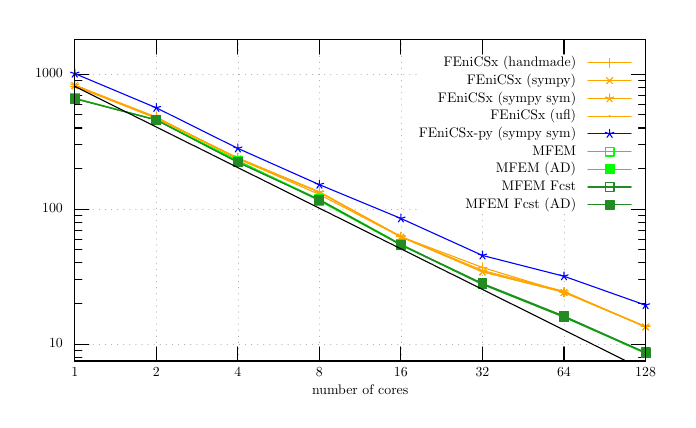
\begin{tikzpicture}[gnuplot]
%% generated with GNUPLOT 6.0p1 (Lua 5.4; terminal rev. Jun 2020, script rev. 118)
%% ven. 10 janv. 2025 17:58:53
\tikzset{every node/.append style={scale=0.50}}
\path (0.000,0.000) rectangle (8.125,4.725);
\gpcolor{color=gp lt color border}
\gpsetlinetype{gp lt border}
\gpsetdashtype{gp dt solid}
\gpsetlinewidth{1.00}
\draw[gp path] (0.598,0.540)--(0.688,0.540);
\draw[gp path] (7.848,0.540)--(7.758,0.540);
\draw[gp path] (0.598,0.628)--(0.688,0.628);
\draw[gp path] (7.848,0.628)--(7.758,0.628);
\gpcolor{color=gp lt color axes}
\gpsetlinetype{gp lt axes}
\gpsetdashtype{gp dt axes}
\gpsetlinewidth{0.50}
\draw[gp path] (0.598,0.706)--(7.848,0.706);
\gpcolor{color=gp lt color border}
\gpsetlinetype{gp lt border}
\gpsetdashtype{gp dt solid}
\gpsetlinewidth{1.00}
\draw[gp path] (0.598,0.706)--(0.778,0.706);
\draw[gp path] (7.848,0.706)--(7.668,0.706);
\node[gp node right] at (0.506,0.706) {$10$};
\draw[gp path] (0.598,1.222)--(0.688,1.222);
\draw[gp path] (7.848,1.222)--(7.758,1.222);
\draw[gp path] (0.598,1.524)--(0.688,1.524);
\draw[gp path] (7.848,1.524)--(7.758,1.524);
\draw[gp path] (0.598,1.738)--(0.688,1.738);
\draw[gp path] (7.848,1.738)--(7.758,1.738);
\draw[gp path] (0.598,1.904)--(0.688,1.904);
\draw[gp path] (7.848,1.904)--(7.758,1.904);
\draw[gp path] (0.598,2.039)--(0.688,2.039);
\draw[gp path] (7.848,2.039)--(7.758,2.039);
\draw[gp path] (0.598,2.154)--(0.688,2.154);
\draw[gp path] (7.848,2.154)--(7.758,2.154);
\draw[gp path] (0.598,2.253)--(0.688,2.253);
\draw[gp path] (7.848,2.253)--(7.758,2.253);
\draw[gp path] (0.598,2.341)--(0.688,2.341);
\draw[gp path] (7.848,2.341)--(7.758,2.341);
\gpcolor{color=gp lt color axes}
\gpsetlinetype{gp lt axes}
\gpsetdashtype{gp dt axes}
\gpsetlinewidth{0.50}
\draw[gp path] (0.598,2.419)--(5.000,2.419);
\draw[gp path] (7.756,2.419)--(7.848,2.419);
\gpcolor{color=gp lt color border}
\gpsetlinetype{gp lt border}
\gpsetdashtype{gp dt solid}
\gpsetlinewidth{1.00}
\draw[gp path] (0.598,2.419)--(0.778,2.419);
\draw[gp path] (7.848,2.419)--(7.668,2.419);
\node[gp node right] at (0.506,2.419) {$100$};
\draw[gp path] (0.598,2.935)--(0.688,2.935);
\draw[gp path] (7.848,2.935)--(7.758,2.935);
\draw[gp path] (0.598,3.237)--(0.688,3.237);
\draw[gp path] (7.848,3.237)--(7.758,3.237);
\draw[gp path] (0.598,3.451)--(0.688,3.451);
\draw[gp path] (7.848,3.451)--(7.758,3.451);
\draw[gp path] (0.598,3.617)--(0.688,3.617);
\draw[gp path] (7.848,3.617)--(7.758,3.617);
\draw[gp path] (0.598,3.753)--(0.688,3.753);
\draw[gp path] (7.848,3.753)--(7.758,3.753);
\draw[gp path] (0.598,3.867)--(0.688,3.867);
\draw[gp path] (7.848,3.867)--(7.758,3.867);
\draw[gp path] (0.598,3.967)--(0.688,3.967);
\draw[gp path] (7.848,3.967)--(7.758,3.967);
\draw[gp path] (0.598,4.054)--(0.688,4.054);
\draw[gp path] (7.848,4.054)--(7.758,4.054);
\gpcolor{color=gp lt color axes}
\gpsetlinetype{gp lt axes}
\gpsetdashtype{gp dt axes}
\gpsetlinewidth{0.50}
\draw[gp path] (0.598,4.133)--(5.000,4.133);
\draw[gp path] (7.756,4.133)--(7.848,4.133);
\gpcolor{color=gp lt color border}
\gpsetlinetype{gp lt border}
\gpsetdashtype{gp dt solid}
\gpsetlinewidth{1.00}
\draw[gp path] (0.598,4.133)--(0.778,4.133);
\draw[gp path] (7.848,4.133)--(7.668,4.133);
\node[gp node right] at (0.506,4.133) {$1000$};
\gpcolor{color=gp lt color axes}
\gpsetlinetype{gp lt axes}
\gpsetdashtype{gp dt axes}
\gpsetlinewidth{0.50}
\draw[gp path] (0.598,0.492)--(0.598,4.570);
\gpcolor{color=gp lt color border}
\gpsetlinetype{gp lt border}
\gpsetdashtype{gp dt solid}
\gpsetlinewidth{1.00}
\draw[gp path] (0.598,0.492)--(0.598,0.672);
\draw[gp path] (0.598,4.570)--(0.598,4.390);
\node[gp node center] at (0.598,0.338) {1};
\gpcolor{color=gp lt color axes}
\gpsetlinetype{gp lt axes}
\gpsetdashtype{gp dt axes}
\gpsetlinewidth{0.50}
\draw[gp path] (1.634,0.492)--(1.634,4.570);
\gpcolor{color=gp lt color border}
\gpsetlinetype{gp lt border}
\gpsetdashtype{gp dt solid}
\gpsetlinewidth{1.00}
\draw[gp path] (1.634,0.492)--(1.634,0.672);
\draw[gp path] (1.634,4.570)--(1.634,4.390);
\node[gp node center] at (1.634,0.338) {2};
\gpcolor{color=gp lt color axes}
\gpsetlinetype{gp lt axes}
\gpsetdashtype{gp dt axes}
\gpsetlinewidth{0.50}
\draw[gp path] (2.669,0.492)--(2.669,4.570);
\gpcolor{color=gp lt color border}
\gpsetlinetype{gp lt border}
\gpsetdashtype{gp dt solid}
\gpsetlinewidth{1.00}
\draw[gp path] (2.669,0.492)--(2.669,0.672);
\draw[gp path] (2.669,4.570)--(2.669,4.390);
\node[gp node center] at (2.669,0.338) {4};
\gpcolor{color=gp lt color axes}
\gpsetlinetype{gp lt axes}
\gpsetdashtype{gp dt axes}
\gpsetlinewidth{0.50}
\draw[gp path] (3.705,0.492)--(3.705,4.570);
\gpcolor{color=gp lt color border}
\gpsetlinetype{gp lt border}
\gpsetdashtype{gp dt solid}
\gpsetlinewidth{1.00}
\draw[gp path] (3.705,0.492)--(3.705,0.672);
\draw[gp path] (3.705,4.570)--(3.705,4.390);
\node[gp node center] at (3.705,0.338) {8};
\gpcolor{color=gp lt color axes}
\gpsetlinetype{gp lt axes}
\gpsetdashtype{gp dt axes}
\gpsetlinewidth{0.50}
\draw[gp path] (4.740,0.492)--(4.740,4.570);
\gpcolor{color=gp lt color border}
\gpsetlinetype{gp lt border}
\gpsetdashtype{gp dt solid}
\gpsetlinewidth{1.00}
\draw[gp path] (4.740,0.492)--(4.740,0.672);
\draw[gp path] (4.740,4.570)--(4.740,4.390);
\node[gp node center] at (4.740,0.338) {16};
\gpcolor{color=gp lt color axes}
\gpsetlinetype{gp lt axes}
\gpsetdashtype{gp dt axes}
\gpsetlinewidth{0.50}
\draw[gp path] (5.776,0.492)--(5.776,2.365);
\draw[gp path] (5.776,4.390)--(5.776,4.570);
\gpcolor{color=gp lt color border}
\gpsetlinetype{gp lt border}
\gpsetdashtype{gp dt solid}
\gpsetlinewidth{1.00}
\draw[gp path] (5.776,0.492)--(5.776,0.672);
\draw[gp path] (5.776,4.570)--(5.776,4.390);
\node[gp node center] at (5.776,0.338) {32};
\gpcolor{color=gp lt color axes}
\gpsetlinetype{gp lt axes}
\gpsetdashtype{gp dt axes}
\gpsetlinewidth{0.50}
\draw[gp path] (6.811,0.492)--(6.811,2.365);
\draw[gp path] (6.811,4.390)--(6.811,4.570);
\gpcolor{color=gp lt color border}
\gpsetlinetype{gp lt border}
\gpsetdashtype{gp dt solid}
\gpsetlinewidth{1.00}
\draw[gp path] (6.811,0.492)--(6.811,0.672);
\draw[gp path] (6.811,4.570)--(6.811,4.390);
\node[gp node center] at (6.811,0.338) {64};
\gpcolor{color=gp lt color axes}
\gpsetlinetype{gp lt axes}
\gpsetdashtype{gp dt axes}
\gpsetlinewidth{0.50}
\draw[gp path] (7.847,0.492)--(7.847,4.570);
\gpcolor{color=gp lt color border}
\gpsetlinetype{gp lt border}
\gpsetdashtype{gp dt solid}
\gpsetlinewidth{1.00}
\draw[gp path] (7.847,0.492)--(7.847,0.672);
\draw[gp path] (7.847,4.570)--(7.847,4.390);
\node[gp node center] at (7.847,0.338) {128};
\draw[gp path] (0.598,4.570)--(0.598,0.492)--(7.848,0.492)--(7.848,4.570)--cycle;
\node[gp node right] at (7.024,4.277) {FEniCSx (handmade)};
\gpcolor{rgb color={1.000,0.647,0.000}}
\draw[gp path] (7.116,4.277)--(7.664,4.277);
\draw[gp path] (0.598,3.980)--(1.634,3.577)--(2.669,3.072)--(3.705,2.639)--(4.740,2.070)%
  --(5.776,1.680)--(6.811,1.364)--(7.847,0.926);
\gpsetpointsize{4.00}
\gp3point{gp mark 1}{}{(0.598,3.980)}
\gp3point{gp mark 1}{}{(1.634,3.577)}
\gp3point{gp mark 1}{}{(2.669,3.072)}
\gp3point{gp mark 1}{}{(3.705,2.639)}
\gp3point{gp mark 1}{}{(4.740,2.070)}
\gp3point{gp mark 1}{}{(5.776,1.680)}
\gp3point{gp mark 1}{}{(6.811,1.364)}
\gp3point{gp mark 1}{}{(7.847,0.926)}
\gp3point{gp mark 1}{}{(7.390,4.277)}
\gpcolor{color=gp lt color border}
\node[gp node right] at (7.024,4.052) {FEniCSx (sympy)};
\gpcolor{rgb color={1.000,0.647,0.000}}
\draw[gp path] (7.116,4.052)--(7.664,4.052);
\draw[gp path] (0.598,3.993)--(1.634,3.573)--(2.669,3.063)--(3.705,2.606)--(4.740,2.068)%
  --(5.776,1.624)--(6.811,1.364)--(7.847,0.926);
\gp3point{gp mark 2}{}{(0.598,3.993)}
\gp3point{gp mark 2}{}{(1.634,3.573)}
\gp3point{gp mark 2}{}{(2.669,3.063)}
\gp3point{gp mark 2}{}{(3.705,2.606)}
\gp3point{gp mark 2}{}{(4.740,2.068)}
\gp3point{gp mark 2}{}{(5.776,1.624)}
\gp3point{gp mark 2}{}{(6.811,1.364)}
\gp3point{gp mark 2}{}{(7.847,0.926)}
\gp3point{gp mark 2}{}{(7.390,4.052)}
\gpcolor{color=gp lt color border}
\node[gp node right] at (7.024,3.827) {FEniCSx (sympy sym)};
\gpcolor{rgb color={1.000,0.647,0.000}}
\draw[gp path] (7.116,3.827)--(7.664,3.827);
\draw[gp path] (0.598,3.992)--(1.634,3.590)--(2.669,3.056)--(3.705,2.636)--(4.740,2.069)%
  --(5.776,1.626)--(6.811,1.367)--(7.847,0.930);
\gp3point{gp mark 3}{}{(0.598,3.992)}
\gp3point{gp mark 3}{}{(1.634,3.590)}
\gp3point{gp mark 3}{}{(2.669,3.056)}
\gp3point{gp mark 3}{}{(3.705,2.636)}
\gp3point{gp mark 3}{}{(4.740,2.069)}
\gp3point{gp mark 3}{}{(5.776,1.626)}
\gp3point{gp mark 3}{}{(6.811,1.367)}
\gp3point{gp mark 3}{}{(7.847,0.930)}
\gp3point{gp mark 3}{}{(7.390,3.827)}
\gpcolor{color=gp lt color border}
\node[gp node right] at (7.024,3.602) {FEniCSx (ufl)};
\gpcolor{rgb color={1.000,0.647,0.000}}
\draw[gp path] (7.116,3.602)--(7.664,3.602);
\draw[gp path] (0.598,3.996)--(1.634,3.584)--(2.669,3.065)--(3.705,2.638)--(4.740,2.071)%
  --(5.776,1.641)--(6.811,1.377)--(7.847,0.925);
\gp3point{gp mark 0}{}{(0.598,3.996)}
\gp3point{gp mark 0}{}{(1.634,3.584)}
\gp3point{gp mark 0}{}{(2.669,3.065)}
\gp3point{gp mark 0}{}{(3.705,2.638)}
\gp3point{gp mark 0}{}{(4.740,2.071)}
\gp3point{gp mark 0}{}{(5.776,1.641)}
\gp3point{gp mark 0}{}{(6.811,1.377)}
\gp3point{gp mark 0}{}{(7.847,0.925)}
\gp3point{gp mark 0}{}{(7.390,3.602)}
\gpcolor{color=gp lt color border}
\node[gp node right] at (7.024,3.377) {FEniCSx-py (sympy sym)};
\gpcolor{rgb color={0.000,0.000,1.000}}
\draw[gp path] (7.116,3.377)--(7.664,3.377);
\draw[gp path] (0.598,4.142)--(1.634,3.707)--(2.669,3.192)--(3.705,2.731)--(4.740,2.302)%
  --(5.776,1.832)--(6.811,1.568)--(7.847,1.201);
\gp3point{gp mark 3}{}{(0.598,4.142)}
\gp3point{gp mark 3}{}{(1.634,3.707)}
\gp3point{gp mark 3}{}{(2.669,3.192)}
\gp3point{gp mark 3}{}{(3.705,2.731)}
\gp3point{gp mark 3}{}{(4.740,2.302)}
\gp3point{gp mark 3}{}{(5.776,1.832)}
\gp3point{gp mark 3}{}{(6.811,1.568)}
\gp3point{gp mark 3}{}{(7.847,1.201)}
\gp3point{gp mark 3}{}{(7.390,3.377)}
\gpcolor{color=gp lt color border}
\node[gp node right] at (7.024,3.152) {MFEM};
\gpcolor{rgb color={0.000,1.000,0.000}}
\draw[gp path] (7.116,3.152)--(7.664,3.152);
\draw[gp path] (0.598,3.830)--(1.634,3.554)--(2.669,3.035)--(3.705,2.544)--(4.740,1.976)%
  --(5.776,1.465)--(6.811,1.047)--(7.847,0.595);
\gp3point{gp mark 4}{}{(0.598,3.830)}
\gp3point{gp mark 4}{}{(1.634,3.554)}
\gp3point{gp mark 4}{}{(2.669,3.035)}
\gp3point{gp mark 4}{}{(3.705,2.544)}
\gp3point{gp mark 4}{}{(4.740,1.976)}
\gp3point{gp mark 4}{}{(5.776,1.465)}
\gp3point{gp mark 4}{}{(6.811,1.047)}
\gp3point{gp mark 4}{}{(7.847,0.595)}
\gp3point{gp mark 4}{}{(7.390,3.152)}
\gpcolor{color=gp lt color border}
\node[gp node right] at (7.024,2.927) {MFEM (AD)};
\gpcolor{rgb color={0.000,1.000,0.000}}
\draw[gp path] (7.116,2.927)--(7.664,2.927);
\draw[gp path] (0.598,3.828)--(1.634,3.555)--(2.669,3.037)--(3.705,2.525)--(4.740,1.964)%
  --(5.776,1.465)--(6.811,1.053)--(7.847,0.587);
\gp3point{gp mark 5}{}{(0.598,3.828)}
\gp3point{gp mark 5}{}{(1.634,3.555)}
\gp3point{gp mark 5}{}{(2.669,3.037)}
\gp3point{gp mark 5}{}{(3.705,2.525)}
\gp3point{gp mark 5}{}{(4.740,1.964)}
\gp3point{gp mark 5}{}{(5.776,1.465)}
\gp3point{gp mark 5}{}{(6.811,1.053)}
\gp3point{gp mark 5}{}{(7.847,0.587)}
\gp3point{gp mark 5}{}{(7.390,2.927)}
\gpcolor{color=gp lt color border}
\node[gp node right] at (7.024,2.702) {MFEM Fcst};
\gpcolor{rgb color={0.133,0.545,0.133}}
\draw[gp path] (7.116,2.702)--(7.664,2.702);
\draw[gp path] (0.598,3.822)--(1.634,3.553)--(2.669,3.014)--(3.705,2.538)--(4.740,1.970)%
  --(5.776,1.478)--(6.811,1.063)--(7.847,0.600);
\gp3point{gp mark 4}{}{(0.598,3.822)}
\gp3point{gp mark 4}{}{(1.634,3.553)}
\gp3point{gp mark 4}{}{(2.669,3.014)}
\gp3point{gp mark 4}{}{(3.705,2.538)}
\gp3point{gp mark 4}{}{(4.740,1.970)}
\gp3point{gp mark 4}{}{(5.776,1.478)}
\gp3point{gp mark 4}{}{(6.811,1.063)}
\gp3point{gp mark 4}{}{(7.847,0.600)}
\gp3point{gp mark 4}{}{(7.390,2.702)}
\gpcolor{color=gp lt color border}
\node[gp node right] at (7.024,2.477) {MFEM Fcst (AD)};
\gpcolor{rgb color={0.133,0.545,0.133}}
\draw[gp path] (7.116,2.477)--(7.664,2.477);
\draw[gp path] (0.598,3.825)--(1.634,3.552)--(2.669,3.016)--(3.705,2.539)--(4.740,1.966)%
  --(5.776,1.466)--(6.811,1.051)--(7.847,0.594);
\gp3point{gp mark 5}{}{(0.598,3.825)}
\gp3point{gp mark 5}{}{(1.634,3.552)}
\gp3point{gp mark 5}{}{(2.669,3.016)}
\gp3point{gp mark 5}{}{(3.705,2.539)}
\gp3point{gp mark 5}{}{(4.740,1.966)}
\gp3point{gp mark 5}{}{(5.776,1.466)}
\gp3point{gp mark 5}{}{(6.811,1.051)}
\gp3point{gp mark 5}{}{(7.847,0.594)}
\gp3point{gp mark 5}{}{(7.390,2.477)}
\gpcolor{rgb color={0.000,0.000,0.000}}
\draw[gp path] (0.598,3.980)--(0.671,3.943)--(0.744,3.907)--(0.818,3.870)--(0.891,3.834)%
  --(0.964,3.797)--(1.037,3.761)--(1.111,3.724)--(1.184,3.688)--(1.257,3.651)--(1.330,3.615)%
  --(1.403,3.578)--(1.477,3.542)--(1.550,3.505)--(1.623,3.469)--(1.696,3.433)--(1.770,3.396)%
  --(1.843,3.360)--(1.916,3.323)--(1.989,3.287)--(2.062,3.250)--(2.136,3.214)--(2.209,3.177)%
  --(2.282,3.141)--(2.355,3.104)--(2.429,3.068)--(2.502,3.031)--(2.575,2.995)--(2.648,2.958)%
  --(2.721,2.922)--(2.795,2.885)--(2.868,2.849)--(2.941,2.813)--(3.014,2.776)--(3.087,2.740)%
  --(3.161,2.703)--(3.234,2.667)--(3.307,2.630)--(3.380,2.594)--(3.454,2.557)--(3.527,2.521)%
  --(3.600,2.484)--(3.673,2.448)--(3.746,2.411)--(3.820,2.375)--(3.893,2.338)--(3.966,2.302)%
  --(4.039,2.266)--(4.113,2.229)--(4.186,2.193)--(4.259,2.156)--(4.332,2.120)--(4.405,2.083)%
  --(4.479,2.047)--(4.552,2.010)--(4.625,1.974)--(4.698,1.937)--(4.772,1.901)--(4.845,1.864)%
  --(4.918,1.828)--(4.991,1.791)--(5.064,1.755)--(5.138,1.719)--(5.211,1.682)--(5.284,1.646)%
  --(5.357,1.609)--(5.431,1.573)--(5.504,1.536)--(5.577,1.500)--(5.650,1.463)--(5.723,1.427)%
  --(5.797,1.390)--(5.870,1.354)--(5.943,1.317)--(6.016,1.281)--(6.090,1.244)--(6.163,1.208)%
  --(6.236,1.172)--(6.309,1.135)--(6.382,1.099)--(6.456,1.062)--(6.529,1.026)--(6.602,0.989)%
  --(6.675,0.953)--(6.749,0.916)--(6.822,0.880)--(6.895,0.843)--(6.968,0.807)--(7.041,0.770)%
  --(7.115,0.734)--(7.188,0.697)--(7.261,0.661)--(7.334,0.625)--(7.408,0.588)--(7.481,0.552)%
  --(7.554,0.515)--(7.600,0.492);
\gpcolor{color=gp lt color border}
\draw[gp path] (0.598,4.570)--(0.598,0.492)--(7.848,0.492)--(7.848,4.570)--cycle;
\node[gp node center] at (4.223,0.107) {number of cores};
%% coordinates of the plot area
\gpdefrectangularnode{gp plot 1}{\pgfpoint{0.598cm}{0.492cm}}{\pgfpoint{7.848cm}{4.570cm}}
\end{tikzpicture}
%% gnuplot variables

		\label{time_simu}
	}
	\subfloat[Simulation (Ratio vs MFEM)]{	
		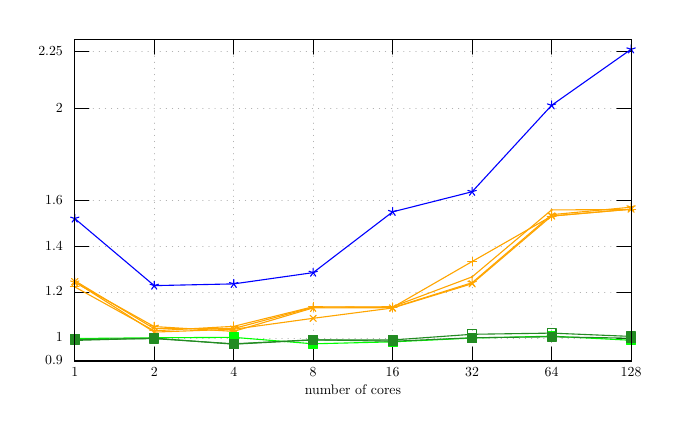
\begin{tikzpicture}[gnuplot]
%% generated with GNUPLOT 6.0p1 (Lua 5.4; terminal rev. Jun 2020, script rev. 118)
%% ven. 10 janv. 2025 17:58:53
\tikzset{every node/.append style={scale=0.50}}
\path (0.000,0.000) rectangle (8.125,4.725);
\gpcolor{color=gp lt color axes}
\gpsetlinetype{gp lt axes}
\gpsetdashtype{gp dt axes}
\gpsetlinewidth{0.50}
\draw[gp path] (0.598,0.492)--(7.664,0.492);
\gpcolor{color=gp lt color border}
\gpsetlinetype{gp lt border}
\gpsetdashtype{gp dt solid}
\gpsetlinewidth{1.00}
\draw[gp path] (0.598,0.492)--(0.778,0.492);
\draw[gp path] (7.664,0.492)--(7.484,0.492);
\node[gp node right] at (0.506,0.492) {$0.9$};
\gpcolor{color=gp lt color axes}
\gpsetlinetype{gp lt axes}
\gpsetdashtype{gp dt axes}
\gpsetlinewidth{0.50}
\draw[gp path] (0.598,0.783)--(7.664,0.783);
\gpcolor{color=gp lt color border}
\gpsetlinetype{gp lt border}
\gpsetdashtype{gp dt solid}
\gpsetlinewidth{1.00}
\draw[gp path] (0.598,0.783)--(0.778,0.783);
\draw[gp path] (7.664,0.783)--(7.484,0.783);
\node[gp node right] at (0.506,0.783) {$1$};
\gpcolor{color=gp lt color axes}
\gpsetlinetype{gp lt axes}
\gpsetdashtype{gp dt axes}
\gpsetlinewidth{0.50}
\draw[gp path] (0.598,1.366)--(7.664,1.366);
\gpcolor{color=gp lt color border}
\gpsetlinetype{gp lt border}
\gpsetdashtype{gp dt solid}
\gpsetlinewidth{1.00}
\draw[gp path] (0.598,1.366)--(0.778,1.366);
\draw[gp path] (7.664,1.366)--(7.484,1.366);
\node[gp node right] at (0.506,1.366) {$1.2$};
\gpcolor{color=gp lt color axes}
\gpsetlinetype{gp lt axes}
\gpsetdashtype{gp dt axes}
\gpsetlinewidth{0.50}
\draw[gp path] (0.598,1.948)--(7.664,1.948);
\gpcolor{color=gp lt color border}
\gpsetlinetype{gp lt border}
\gpsetdashtype{gp dt solid}
\gpsetlinewidth{1.00}
\draw[gp path] (0.598,1.948)--(0.778,1.948);
\draw[gp path] (7.664,1.948)--(7.484,1.948);
\node[gp node right] at (0.506,1.948) {$1.4$};
\gpcolor{color=gp lt color axes}
\gpsetlinetype{gp lt axes}
\gpsetdashtype{gp dt axes}
\gpsetlinewidth{0.50}
\draw[gp path] (0.598,2.531)--(7.664,2.531);
\gpcolor{color=gp lt color border}
\gpsetlinetype{gp lt border}
\gpsetdashtype{gp dt solid}
\gpsetlinewidth{1.00}
\draw[gp path] (0.598,2.531)--(0.778,2.531);
\draw[gp path] (7.664,2.531)--(7.484,2.531);
\node[gp node right] at (0.506,2.531) {$1.6$};
\gpcolor{color=gp lt color axes}
\gpsetlinetype{gp lt axes}
\gpsetdashtype{gp dt axes}
\gpsetlinewidth{0.50}
\draw[gp path] (0.598,3.696)--(7.664,3.696);
\gpcolor{color=gp lt color border}
\gpsetlinetype{gp lt border}
\gpsetdashtype{gp dt solid}
\gpsetlinewidth{1.00}
\draw[gp path] (0.598,3.696)--(0.778,3.696);
\draw[gp path] (7.664,3.696)--(7.484,3.696);
\node[gp node right] at (0.506,3.696) {$2$};
\gpcolor{color=gp lt color axes}
\gpsetlinetype{gp lt axes}
\gpsetdashtype{gp dt axes}
\gpsetlinewidth{0.50}
\draw[gp path] (0.598,4.424)--(7.664,4.424);
\gpcolor{color=gp lt color border}
\gpsetlinetype{gp lt border}
\gpsetdashtype{gp dt solid}
\gpsetlinewidth{1.00}
\draw[gp path] (0.598,4.424)--(0.778,4.424);
\draw[gp path] (7.664,4.424)--(7.484,4.424);
\node[gp node right] at (0.506,4.424) {$2.25$};
\gpcolor{color=gp lt color axes}
\gpsetlinetype{gp lt axes}
\gpsetdashtype{gp dt axes}
\gpsetlinewidth{0.50}
\draw[gp path] (0.598,0.492)--(0.598,4.570);
\gpcolor{color=gp lt color border}
\gpsetlinetype{gp lt border}
\gpsetdashtype{gp dt solid}
\gpsetlinewidth{1.00}
\draw[gp path] (0.598,0.492)--(0.598,0.672);
\draw[gp path] (0.598,4.570)--(0.598,4.390);
\node[gp node center] at (0.598,0.338) {1};
\gpcolor{color=gp lt color axes}
\gpsetlinetype{gp lt axes}
\gpsetdashtype{gp dt axes}
\gpsetlinewidth{0.50}
\draw[gp path] (1.607,0.492)--(1.607,4.570);
\gpcolor{color=gp lt color border}
\gpsetlinetype{gp lt border}
\gpsetdashtype{gp dt solid}
\gpsetlinewidth{1.00}
\draw[gp path] (1.607,0.492)--(1.607,0.672);
\draw[gp path] (1.607,4.570)--(1.607,4.390);
\node[gp node center] at (1.607,0.338) {2};
\gpcolor{color=gp lt color axes}
\gpsetlinetype{gp lt axes}
\gpsetdashtype{gp dt axes}
\gpsetlinewidth{0.50}
\draw[gp path] (2.617,0.492)--(2.617,4.570);
\gpcolor{color=gp lt color border}
\gpsetlinetype{gp lt border}
\gpsetdashtype{gp dt solid}
\gpsetlinewidth{1.00}
\draw[gp path] (2.617,0.492)--(2.617,0.672);
\draw[gp path] (2.617,4.570)--(2.617,4.390);
\node[gp node center] at (2.617,0.338) {4};
\gpcolor{color=gp lt color axes}
\gpsetlinetype{gp lt axes}
\gpsetdashtype{gp dt axes}
\gpsetlinewidth{0.50}
\draw[gp path] (3.626,0.492)--(3.626,4.570);
\gpcolor{color=gp lt color border}
\gpsetlinetype{gp lt border}
\gpsetdashtype{gp dt solid}
\gpsetlinewidth{1.00}
\draw[gp path] (3.626,0.492)--(3.626,0.672);
\draw[gp path] (3.626,4.570)--(3.626,4.390);
\node[gp node center] at (3.626,0.338) {8};
\gpcolor{color=gp lt color axes}
\gpsetlinetype{gp lt axes}
\gpsetdashtype{gp dt axes}
\gpsetlinewidth{0.50}
\draw[gp path] (4.635,0.492)--(4.635,4.570);
\gpcolor{color=gp lt color border}
\gpsetlinetype{gp lt border}
\gpsetdashtype{gp dt solid}
\gpsetlinewidth{1.00}
\draw[gp path] (4.635,0.492)--(4.635,0.672);
\draw[gp path] (4.635,4.570)--(4.635,4.390);
\node[gp node center] at (4.635,0.338) {16};
\gpcolor{color=gp lt color axes}
\gpsetlinetype{gp lt axes}
\gpsetdashtype{gp dt axes}
\gpsetlinewidth{0.50}
\draw[gp path] (5.644,0.492)--(5.644,4.570);
\gpcolor{color=gp lt color border}
\gpsetlinetype{gp lt border}
\gpsetdashtype{gp dt solid}
\gpsetlinewidth{1.00}
\draw[gp path] (5.644,0.492)--(5.644,0.672);
\draw[gp path] (5.644,4.570)--(5.644,4.390);
\node[gp node center] at (5.644,0.338) {32};
\gpcolor{color=gp lt color axes}
\gpsetlinetype{gp lt axes}
\gpsetdashtype{gp dt axes}
\gpsetlinewidth{0.50}
\draw[gp path] (6.654,0.492)--(6.654,4.570);
\gpcolor{color=gp lt color border}
\gpsetlinetype{gp lt border}
\gpsetdashtype{gp dt solid}
\gpsetlinewidth{1.00}
\draw[gp path] (6.654,0.492)--(6.654,0.672);
\draw[gp path] (6.654,4.570)--(6.654,4.390);
\node[gp node center] at (6.654,0.338) {64};
\gpcolor{color=gp lt color axes}
\gpsetlinetype{gp lt axes}
\gpsetdashtype{gp dt axes}
\gpsetlinewidth{0.50}
\draw[gp path] (7.663,0.492)--(7.663,4.570);
\gpcolor{color=gp lt color border}
\gpsetlinetype{gp lt border}
\gpsetdashtype{gp dt solid}
\gpsetlinewidth{1.00}
\draw[gp path] (7.663,0.492)--(7.663,0.672);
\draw[gp path] (7.663,4.570)--(7.663,4.390);
\node[gp node center] at (7.663,0.338) {128};
\draw[gp path] (0.598,4.570)--(0.598,0.492)--(7.664,0.492)--(7.664,4.570)--cycle;
\gpcolor{rgb color={1.000,0.647,0.000}}
\draw[gp path] (0.598,1.433)--(1.607,0.875)--(2.617,0.932)--(3.626,1.181)--(4.635,1.173)%
  --(5.644,1.755)--(6.654,2.332)--(7.663,2.419);
\gpsetpointsize{4.00}
\gp3point{gp mark 1}{}{(0.598,1.433)}
\gp3point{gp mark 1}{}{(1.607,0.875)}
\gp3point{gp mark 1}{}{(2.617,0.932)}
\gp3point{gp mark 1}{}{(3.626,1.181)}
\gp3point{gp mark 1}{}{(4.635,1.173)}
\gp3point{gp mark 1}{}{(5.644,1.755)}
\gp3point{gp mark 1}{}{(6.654,2.332)}
\gp3point{gp mark 1}{}{(7.663,2.419)}
\draw[gp path] (0.598,1.499)--(1.607,0.859)--(2.617,0.895)--(3.626,1.034)--(4.635,1.165)%
  --(5.644,1.473)--(6.654,2.333)--(7.663,2.420);
\gp3point{gp mark 2}{}{(0.598,1.499)}
\gp3point{gp mark 2}{}{(1.607,0.859)}
\gp3point{gp mark 2}{}{(2.617,0.895)}
\gp3point{gp mark 2}{}{(3.626,1.034)}
\gp3point{gp mark 2}{}{(4.635,1.165)}
\gp3point{gp mark 2}{}{(5.644,1.473)}
\gp3point{gp mark 2}{}{(6.654,2.333)}
\gp3point{gp mark 2}{}{(7.663,2.420)}
\draw[gp path] (0.598,1.491)--(1.607,0.929)--(2.617,0.868)--(3.626,1.166)--(4.635,1.169)%
  --(5.644,1.486)--(6.654,2.350)--(7.663,2.445);
\gp3point{gp mark 3}{}{(0.598,1.491)}
\gp3point{gp mark 3}{}{(1.607,0.929)}
\gp3point{gp mark 3}{}{(2.617,0.868)}
\gp3point{gp mark 3}{}{(3.626,1.166)}
\gp3point{gp mark 3}{}{(4.635,1.169)}
\gp3point{gp mark 3}{}{(5.644,1.486)}
\gp3point{gp mark 3}{}{(6.654,2.350)}
\gp3point{gp mark 3}{}{(7.663,2.445)}
\draw[gp path] (0.598,1.512)--(1.607,0.902)--(2.617,0.904)--(3.626,1.174)--(4.635,1.181)%
  --(5.644,1.560)--(6.654,2.411)--(7.663,2.414);
\gp3point{gp mark 0}{}{(0.598,1.512)}
\gp3point{gp mark 0}{}{(1.607,0.902)}
\gp3point{gp mark 0}{}{(2.617,0.904)}
\gp3point{gp mark 0}{}{(3.626,1.174)}
\gp3point{gp mark 0}{}{(4.635,1.181)}
\gp3point{gp mark 0}{}{(5.644,1.560)}
\gp3point{gp mark 0}{}{(6.654,2.411)}
\gp3point{gp mark 0}{}{(7.663,2.414)}
\gpcolor{rgb color={0.000,0.000,1.000}}
\draw[gp path] (0.598,2.301)--(1.607,1.449)--(2.617,1.471)--(3.626,1.614)--(4.635,2.386)%
  --(5.644,2.641)--(6.654,3.739)--(7.663,4.450);
\gp3point{gp mark 3}{}{(0.598,2.301)}
\gp3point{gp mark 3}{}{(1.607,1.449)}
\gp3point{gp mark 3}{}{(2.617,1.471)}
\gp3point{gp mark 3}{}{(3.626,1.614)}
\gp3point{gp mark 3}{}{(4.635,2.386)}
\gp3point{gp mark 3}{}{(5.644,2.641)}
\gp3point{gp mark 3}{}{(6.654,3.739)}
\gp3point{gp mark 3}{}{(7.663,4.450)}
\gpcolor{rgb color={0.000,1.000,0.000}}
\draw[gp path] (0.598,0.777)--(1.607,0.787)--(2.617,0.792)--(3.626,0.710)--(4.635,0.735)%
  --(5.644,0.783)--(6.654,0.807)--(7.663,0.755);
\gp3point{gp mark 5}{}{(0.598,0.777)}
\gp3point{gp mark 5}{}{(1.607,0.787)}
\gp3point{gp mark 5}{}{(2.617,0.792)}
\gp3point{gp mark 5}{}{(3.626,0.710)}
\gp3point{gp mark 5}{}{(4.635,0.735)}
\gp3point{gp mark 5}{}{(5.644,0.783)}
\gp3point{gp mark 5}{}{(6.654,0.807)}
\gp3point{gp mark 5}{}{(7.663,0.755)}
\gpcolor{rgb color={0.133,0.545,0.133}}
\draw[gp path] (0.598,0.753)--(1.607,0.782)--(2.617,0.705)--(3.626,0.759)--(4.635,0.759)%
  --(5.644,0.831)--(6.654,0.846)--(7.663,0.804);
\gp3point{gp mark 4}{}{(0.598,0.753)}
\gp3point{gp mark 4}{}{(1.607,0.782)}
\gp3point{gp mark 4}{}{(2.617,0.705)}
\gp3point{gp mark 4}{}{(3.626,0.759)}
\gp3point{gp mark 4}{}{(4.635,0.759)}
\gp3point{gp mark 4}{}{(5.644,0.831)}
\gp3point{gp mark 4}{}{(6.654,0.846)}
\gp3point{gp mark 4}{}{(7.663,0.804)}
\draw[gp path] (0.598,0.766)--(1.607,0.776)--(2.617,0.710)--(3.626,0.762)--(4.635,0.742)%
  --(5.644,0.787)--(6.654,0.799)--(7.663,0.781);
\gp3point{gp mark 5}{}{(0.598,0.766)}
\gp3point{gp mark 5}{}{(1.607,0.776)}
\gp3point{gp mark 5}{}{(2.617,0.710)}
\gp3point{gp mark 5}{}{(3.626,0.762)}
\gp3point{gp mark 5}{}{(4.635,0.742)}
\gp3point{gp mark 5}{}{(5.644,0.787)}
\gp3point{gp mark 5}{}{(6.654,0.799)}
\gp3point{gp mark 5}{}{(7.663,0.781)}
\gpcolor{color=gp lt color border}
\draw[gp path] (0.598,4.570)--(0.598,0.492)--(7.664,0.492)--(7.664,4.570)--cycle;
\node[gp node center] at (4.131,0.107) {number of cores};
%% coordinates of the plot area
\gpdefrectangularnode{gp plot 1}{\pgfpoint{0.598cm}{0.492cm}}{\pgfpoint{7.664cm}{4.570cm}}
\end{tikzpicture}
%% gnuplot variables

		\label{time_simu_r}
	}\\
	\subfloat[Mesh (in s)]{
		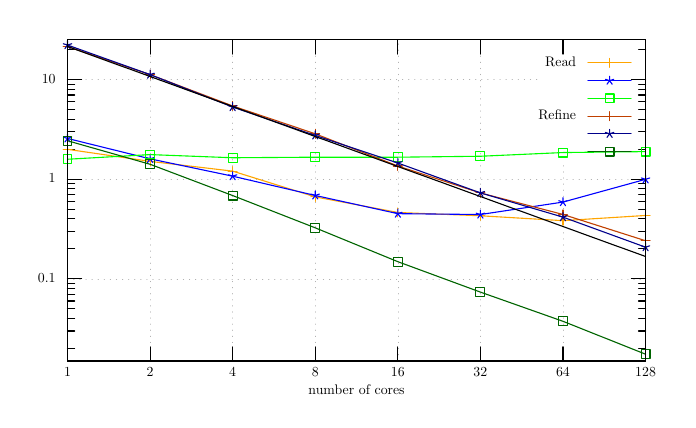
\begin{tikzpicture}[gnuplot]
%% generated with GNUPLOT 6.0p1 (Lua 5.4; terminal rev. Jun 2020, script rev. 118)
%% ven. 10 janv. 2025 17:58:53
\tikzset{every node/.append style={scale=0.50}}
\path (0.000,0.000) rectangle (8.125,4.725);
\gpcolor{color=gp lt color border}
\gpsetlinetype{gp lt border}
\gpsetdashtype{gp dt solid}
\gpsetlinewidth{1.00}
\draw[gp path] (0.506,0.650)--(0.596,0.650);
\draw[gp path] (7.848,0.650)--(7.758,0.650);
\draw[gp path] (0.506,0.873)--(0.596,0.873);
\draw[gp path] (7.848,0.873)--(7.758,0.873);
\draw[gp path] (0.506,1.031)--(0.596,1.031);
\draw[gp path] (7.848,1.031)--(7.758,1.031);
\draw[gp path] (0.506,1.154)--(0.596,1.154);
\draw[gp path] (7.848,1.154)--(7.758,1.154);
\draw[gp path] (0.506,1.254)--(0.596,1.254);
\draw[gp path] (7.848,1.254)--(7.758,1.254);
\draw[gp path] (0.506,1.339)--(0.596,1.339);
\draw[gp path] (7.848,1.339)--(7.758,1.339);
\draw[gp path] (0.506,1.412)--(0.596,1.412);
\draw[gp path] (7.848,1.412)--(7.758,1.412);
\draw[gp path] (0.506,1.477)--(0.596,1.477);
\draw[gp path] (7.848,1.477)--(7.758,1.477);
\gpcolor{color=gp lt color axes}
\gpsetlinetype{gp lt axes}
\gpsetdashtype{gp dt axes}
\gpsetlinewidth{0.50}
\draw[gp path] (0.506,1.535)--(7.848,1.535);
\gpcolor{color=gp lt color border}
\gpsetlinetype{gp lt border}
\gpsetdashtype{gp dt solid}
\gpsetlinewidth{1.00}
\draw[gp path] (0.506,1.535)--(0.686,1.535);
\draw[gp path] (7.848,1.535)--(7.668,1.535);
\node[gp node right] at (0.414,1.535) {$0.1$};
\draw[gp path] (0.506,1.916)--(0.596,1.916);
\draw[gp path] (7.848,1.916)--(7.758,1.916);
\draw[gp path] (0.506,2.139)--(0.596,2.139);
\draw[gp path] (7.848,2.139)--(7.758,2.139);
\draw[gp path] (0.506,2.297)--(0.596,2.297);
\draw[gp path] (7.848,2.297)--(7.758,2.297);
\draw[gp path] (0.506,2.420)--(0.596,2.420);
\draw[gp path] (7.848,2.420)--(7.758,2.420);
\draw[gp path] (0.506,2.520)--(0.596,2.520);
\draw[gp path] (7.848,2.520)--(7.758,2.520);
\draw[gp path] (0.506,2.605)--(0.596,2.605);
\draw[gp path] (7.848,2.605)--(7.758,2.605);
\draw[gp path] (0.506,2.678)--(0.596,2.678);
\draw[gp path] (7.848,2.678)--(7.758,2.678);
\draw[gp path] (0.506,2.743)--(0.596,2.743);
\draw[gp path] (7.848,2.743)--(7.758,2.743);
\gpcolor{color=gp lt color axes}
\gpsetlinetype{gp lt axes}
\gpsetdashtype{gp dt axes}
\gpsetlinewidth{0.50}
\draw[gp path] (0.506,2.801)--(7.848,2.801);
\gpcolor{color=gp lt color border}
\gpsetlinetype{gp lt border}
\gpsetdashtype{gp dt solid}
\gpsetlinewidth{1.00}
\draw[gp path] (0.506,2.801)--(0.686,2.801);
\draw[gp path] (7.848,2.801)--(7.668,2.801);
\node[gp node right] at (0.414,2.801) {$1$};
\draw[gp path] (0.506,3.182)--(0.596,3.182);
\draw[gp path] (7.848,3.182)--(7.758,3.182);
\draw[gp path] (0.506,3.404)--(0.596,3.404);
\draw[gp path] (7.848,3.404)--(7.758,3.404);
\draw[gp path] (0.506,3.563)--(0.596,3.563);
\draw[gp path] (7.848,3.563)--(7.758,3.563);
\draw[gp path] (0.506,3.685)--(0.596,3.685);
\draw[gp path] (7.848,3.685)--(7.758,3.685);
\draw[gp path] (0.506,3.786)--(0.596,3.786);
\draw[gp path] (7.848,3.786)--(7.758,3.786);
\draw[gp path] (0.506,3.870)--(0.596,3.870);
\draw[gp path] (7.848,3.870)--(7.758,3.870);
\draw[gp path] (0.506,3.944)--(0.596,3.944);
\draw[gp path] (7.848,3.944)--(7.758,3.944);
\draw[gp path] (0.506,4.008)--(0.596,4.008);
\draw[gp path] (7.848,4.008)--(7.758,4.008);
\gpcolor{color=gp lt color axes}
\gpsetlinetype{gp lt axes}
\gpsetdashtype{gp dt axes}
\gpsetlinewidth{0.50}
\draw[gp path] (0.506,4.066)--(6.472,4.066);
\draw[gp path] (7.756,4.066)--(7.848,4.066);
\gpcolor{color=gp lt color border}
\gpsetlinetype{gp lt border}
\gpsetdashtype{gp dt solid}
\gpsetlinewidth{1.00}
\draw[gp path] (0.506,4.066)--(0.686,4.066);
\draw[gp path] (7.848,4.066)--(7.668,4.066);
\node[gp node right] at (0.414,4.066) {$10$};
\draw[gp path] (0.506,4.447)--(0.596,4.447);
\draw[gp path] (7.848,4.447)--(7.758,4.447);
\gpcolor{color=gp lt color axes}
\gpsetlinetype{gp lt axes}
\gpsetdashtype{gp dt axes}
\gpsetlinewidth{0.50}
\draw[gp path] (0.506,0.492)--(0.506,4.570);
\gpcolor{color=gp lt color border}
\gpsetlinetype{gp lt border}
\gpsetdashtype{gp dt solid}
\gpsetlinewidth{1.00}
\draw[gp path] (0.506,0.492)--(0.506,0.672);
\draw[gp path] (0.506,4.570)--(0.506,4.390);
\node[gp node center] at (0.506,0.338) {1};
\gpcolor{color=gp lt color axes}
\gpsetlinetype{gp lt axes}
\gpsetdashtype{gp dt axes}
\gpsetlinewidth{0.50}
\draw[gp path] (1.555,0.492)--(1.555,4.570);
\gpcolor{color=gp lt color border}
\gpsetlinetype{gp lt border}
\gpsetdashtype{gp dt solid}
\gpsetlinewidth{1.00}
\draw[gp path] (1.555,0.492)--(1.555,0.672);
\draw[gp path] (1.555,4.570)--(1.555,4.390);
\node[gp node center] at (1.555,0.338) {2};
\gpcolor{color=gp lt color axes}
\gpsetlinetype{gp lt axes}
\gpsetdashtype{gp dt axes}
\gpsetlinewidth{0.50}
\draw[gp path] (2.603,0.492)--(2.603,4.570);
\gpcolor{color=gp lt color border}
\gpsetlinetype{gp lt border}
\gpsetdashtype{gp dt solid}
\gpsetlinewidth{1.00}
\draw[gp path] (2.603,0.492)--(2.603,0.672);
\draw[gp path] (2.603,4.570)--(2.603,4.390);
\node[gp node center] at (2.603,0.338) {4};
\gpcolor{color=gp lt color axes}
\gpsetlinetype{gp lt axes}
\gpsetdashtype{gp dt axes}
\gpsetlinewidth{0.50}
\draw[gp path] (3.652,0.492)--(3.652,4.570);
\gpcolor{color=gp lt color border}
\gpsetlinetype{gp lt border}
\gpsetdashtype{gp dt solid}
\gpsetlinewidth{1.00}
\draw[gp path] (3.652,0.492)--(3.652,0.672);
\draw[gp path] (3.652,4.570)--(3.652,4.390);
\node[gp node center] at (3.652,0.338) {8};
\gpcolor{color=gp lt color axes}
\gpsetlinetype{gp lt axes}
\gpsetdashtype{gp dt axes}
\gpsetlinewidth{0.50}
\draw[gp path] (4.701,0.492)--(4.701,4.570);
\gpcolor{color=gp lt color border}
\gpsetlinetype{gp lt border}
\gpsetdashtype{gp dt solid}
\gpsetlinewidth{1.00}
\draw[gp path] (4.701,0.492)--(4.701,0.672);
\draw[gp path] (4.701,4.570)--(4.701,4.390);
\node[gp node center] at (4.701,0.338) {16};
\gpcolor{color=gp lt color axes}
\gpsetlinetype{gp lt axes}
\gpsetdashtype{gp dt axes}
\gpsetlinewidth{0.50}
\draw[gp path] (5.749,0.492)--(5.749,4.570);
\gpcolor{color=gp lt color border}
\gpsetlinetype{gp lt border}
\gpsetdashtype{gp dt solid}
\gpsetlinewidth{1.00}
\draw[gp path] (5.749,0.492)--(5.749,0.672);
\draw[gp path] (5.749,4.570)--(5.749,4.390);
\node[gp node center] at (5.749,0.338) {32};
\gpcolor{color=gp lt color axes}
\gpsetlinetype{gp lt axes}
\gpsetdashtype{gp dt axes}
\gpsetlinewidth{0.50}
\draw[gp path] (6.798,0.492)--(6.798,3.040);
\draw[gp path] (6.798,4.390)--(6.798,4.570);
\gpcolor{color=gp lt color border}
\gpsetlinetype{gp lt border}
\gpsetdashtype{gp dt solid}
\gpsetlinewidth{1.00}
\draw[gp path] (6.798,0.492)--(6.798,0.672);
\draw[gp path] (6.798,4.570)--(6.798,4.390);
\node[gp node center] at (6.798,0.338) {64};
\gpcolor{color=gp lt color axes}
\gpsetlinetype{gp lt axes}
\gpsetdashtype{gp dt axes}
\gpsetlinewidth{0.50}
\draw[gp path] (7.847,0.492)--(7.847,4.570);
\gpcolor{color=gp lt color border}
\gpsetlinetype{gp lt border}
\gpsetdashtype{gp dt solid}
\gpsetlinewidth{1.00}
\draw[gp path] (7.847,0.492)--(7.847,0.672);
\draw[gp path] (7.847,4.570)--(7.847,4.390);
\node[gp node center] at (7.847,0.338) {128};
\draw[gp path] (0.506,4.570)--(0.506,0.492)--(7.848,0.492)--(7.848,4.570)--cycle;
\node[gp node right] at (7.024,4.277) {Read};
\gpcolor{rgb color={1.000,0.647,0.000}}
\draw[gp path] (7.116,4.277)--(7.664,4.277);
\draw[gp path] (0.506,3.180)--(1.555,3.027)--(2.603,2.903)--(3.652,2.576)--(4.701,2.378)%
  --(5.749,2.336)--(6.798,2.274)--(7.847,2.340);
\gpsetpointsize{4.00}
\gp3point{gp mark 1}{}{(0.506,3.180)}
\gp3point{gp mark 1}{}{(1.555,3.027)}
\gp3point{gp mark 1}{}{(2.603,2.903)}
\gp3point{gp mark 1}{}{(3.652,2.576)}
\gp3point{gp mark 1}{}{(4.701,2.378)}
\gp3point{gp mark 1}{}{(5.749,2.336)}
\gp3point{gp mark 1}{}{(6.798,2.274)}
\gp3point{gp mark 1}{}{(7.847,2.340)}
\gp3point{gp mark 1}{}{(7.390,4.277)}
\gpcolor{color=gp lt color border}
\node[gp node right] at (7.024,4.052) { };
\gpcolor{rgb color={0.000,0.000,1.000}}
\draw[gp path] (7.116,4.052)--(7.664,4.052);
\draw[gp path] (0.506,3.318)--(1.555,3.059)--(2.603,2.839)--(3.652,2.594)--(4.701,2.363)%
  --(5.749,2.352)--(6.798,2.510)--(7.847,2.799);
\gp3point{gp mark 3}{}{(0.506,3.318)}
\gp3point{gp mark 3}{}{(1.555,3.059)}
\gp3point{gp mark 3}{}{(2.603,2.839)}
\gp3point{gp mark 3}{}{(3.652,2.594)}
\gp3point{gp mark 3}{}{(4.701,2.363)}
\gp3point{gp mark 3}{}{(5.749,2.352)}
\gp3point{gp mark 3}{}{(6.798,2.510)}
\gp3point{gp mark 3}{}{(7.847,2.799)}
\gp3point{gp mark 3}{}{(7.390,4.052)}
\gpcolor{color=gp lt color border}
\node[gp node right] at (7.024,3.827) { };
\gpcolor{rgb color={0.000,1.000,0.000}}
\draw[gp path] (7.116,3.827)--(7.664,3.827);
\draw[gp path] (0.506,3.054)--(1.555,3.113)--(2.603,3.073)--(3.652,3.080)--(4.701,3.080)%
  --(5.749,3.092)--(6.798,3.139)--(7.847,3.151);
\gp3point{gp mark 4}{}{(0.506,3.054)}
\gp3point{gp mark 4}{}{(1.555,3.113)}
\gp3point{gp mark 4}{}{(2.603,3.073)}
\gp3point{gp mark 4}{}{(3.652,3.080)}
\gp3point{gp mark 4}{}{(4.701,3.080)}
\gp3point{gp mark 4}{}{(5.749,3.092)}
\gp3point{gp mark 4}{}{(6.798,3.139)}
\gp3point{gp mark 4}{}{(7.847,3.151)}
\gp3point{gp mark 4}{}{(7.390,3.827)}
\gpcolor{color=gp lt color border}
\node[gp node right] at (7.024,3.602) {Refine};
\gpcolor{rgb color={0.753,0.251,0.000}}
\draw[gp path] (7.116,3.602)--(7.664,3.602);
\draw[gp path] (0.506,4.486)--(1.555,4.128)--(2.603,3.731)--(3.652,3.377)--(4.701,2.968)%
  --(5.749,2.626)--(6.798,2.353)--(7.847,2.019);
\gp3point{gp mark 1}{}{(0.506,4.486)}
\gp3point{gp mark 1}{}{(1.555,4.128)}
\gp3point{gp mark 1}{}{(2.603,3.731)}
\gp3point{gp mark 1}{}{(3.652,3.377)}
\gp3point{gp mark 1}{}{(4.701,2.968)}
\gp3point{gp mark 1}{}{(5.749,2.626)}
\gp3point{gp mark 1}{}{(6.798,2.353)}
\gp3point{gp mark 1}{}{(7.847,2.019)}
\gp3point{gp mark 1}{}{(7.390,3.602)}
\gpcolor{color=gp lt color border}
\node[gp node right] at (7.024,3.377) { };
\gpcolor{rgb color={0.000,0.000,0.545}}
\draw[gp path] (7.116,3.377)--(7.664,3.377);
\draw[gp path] (0.506,4.504)--(1.555,4.129)--(2.603,3.717)--(3.652,3.356)--(4.701,3.006)%
  --(5.749,2.627)--(6.798,2.319)--(7.847,1.937);
\gp3point{gp mark 3}{}{(0.506,4.504)}
\gp3point{gp mark 3}{}{(1.555,4.129)}
\gp3point{gp mark 3}{}{(2.603,3.717)}
\gp3point{gp mark 3}{}{(3.652,3.356)}
\gp3point{gp mark 3}{}{(4.701,3.006)}
\gp3point{gp mark 3}{}{(5.749,2.627)}
\gp3point{gp mark 3}{}{(6.798,2.319)}
\gp3point{gp mark 3}{}{(7.847,1.937)}
\gp3point{gp mark 3}{}{(7.390,3.377)}
\gpcolor{color=gp lt color border}
\node[gp node right] at (7.024,3.152) { };
\gpcolor{rgb color={0.000,0.392,0.000}}
\draw[gp path] (7.116,3.152)--(7.664,3.152);
\draw[gp path] (0.506,3.289)--(1.555,2.990)--(2.603,2.593)--(3.652,2.183)--(4.701,1.753)%
  --(5.749,1.367)--(6.798,0.996)--(7.847,0.578);
\gp3point{gp mark 4}{}{(0.506,3.289)}
\gp3point{gp mark 4}{}{(1.555,2.990)}
\gp3point{gp mark 4}{}{(2.603,2.593)}
\gp3point{gp mark 4}{}{(3.652,2.183)}
\gp3point{gp mark 4}{}{(4.701,1.753)}
\gp3point{gp mark 4}{}{(5.749,1.367)}
\gp3point{gp mark 4}{}{(6.798,0.996)}
\gp3point{gp mark 4}{}{(7.847,0.578)}
\gp3point{gp mark 4}{}{(7.390,3.152)}
\gpcolor{rgb color={0.000,0.000,0.000}}
\draw[gp path] (0.506,4.486)--(0.580,4.459)--(0.654,4.432)--(0.728,4.405)--(0.803,4.378)%
  --(0.877,4.351)--(0.951,4.324)--(1.025,4.297)--(1.099,4.270)--(1.173,4.243)--(1.247,4.217)%
  --(1.322,4.190)--(1.396,4.163)--(1.470,4.136)--(1.544,4.109)--(1.618,4.082)--(1.692,4.055)%
  --(1.767,4.028)--(1.841,4.001)--(1.915,3.974)--(1.989,3.947)--(2.063,3.920)--(2.137,3.893)%
  --(2.211,3.866)--(2.286,3.839)--(2.360,3.812)--(2.434,3.785)--(2.508,3.759)--(2.582,3.732)%
  --(2.656,3.705)--(2.730,3.678)--(2.805,3.651)--(2.879,3.624)--(2.953,3.597)--(3.027,3.570)%
  --(3.101,3.543)--(3.175,3.516)--(3.250,3.489)--(3.324,3.462)--(3.398,3.435)--(3.472,3.408)%
  --(3.546,3.381)--(3.620,3.354)--(3.694,3.327)--(3.769,3.301)--(3.843,3.274)--(3.917,3.247)%
  --(3.991,3.220)--(4.065,3.193)--(4.139,3.166)--(4.213,3.139)--(4.288,3.112)--(4.362,3.085)%
  --(4.436,3.058)--(4.510,3.031)--(4.584,3.004)--(4.658,2.977)--(4.733,2.950)--(4.807,2.923)%
  --(4.881,2.896)--(4.955,2.869)--(5.029,2.843)--(5.103,2.816)--(5.177,2.789)--(5.252,2.762)%
  --(5.326,2.735)--(5.400,2.708)--(5.474,2.681)--(5.548,2.654)--(5.622,2.627)--(5.696,2.600)%
  --(5.771,2.573)--(5.845,2.546)--(5.919,2.519)--(5.993,2.492)--(6.067,2.465)--(6.141,2.438)%
  --(6.216,2.411)--(6.290,2.385)--(6.364,2.358)--(6.438,2.331)--(6.512,2.304)--(6.586,2.277)%
  --(6.660,2.250)--(6.735,2.223)--(6.809,2.196)--(6.883,2.169)--(6.957,2.142)--(7.031,2.115)%
  --(7.105,2.088)--(7.179,2.061)--(7.254,2.034)--(7.328,2.007)--(7.402,1.980)--(7.476,1.953)%
  --(7.550,1.927)--(7.624,1.900)--(7.699,1.873)--(7.773,1.846)--(7.847,1.819);
\gpcolor{color=gp lt color border}
\draw[gp path] (0.506,4.570)--(0.506,0.492)--(7.848,0.492)--(7.848,4.570)--cycle;
\node[gp node center] at (4.177,0.107) {number of cores};
%% coordinates of the plot area
\gpdefrectangularnode{gp plot 1}{\pgfpoint{0.506cm}{0.492cm}}{\pgfpoint{7.848cm}{4.570cm}}
\end{tikzpicture}
%% gnuplot variables

		\label{time_mesh}
	}
	\subfloat[Mesh  (Ratio vs MFEM)]{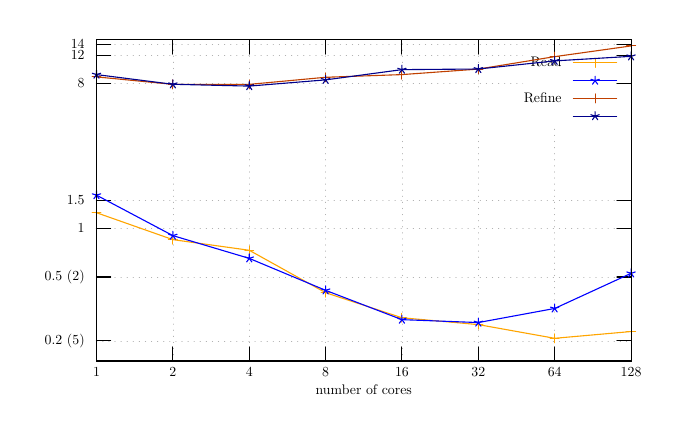
\begin{tikzpicture}[gnuplot]
%% generated with GNUPLOT 6.0p1 (Lua 5.4; terminal rev. Jun 2020, script rev. 118)
%% ven. 10 janv. 2025 17:58:53
\tikzset{every node/.append style={scale=0.50}}
\path (0.000,0.000) rectangle (8.125,4.725);
\gpcolor{color=gp lt color axes}
\gpsetlinetype{gp lt axes}
\gpsetdashtype{gp dt axes}
\gpsetlinewidth{0.50}
\draw[gp path] (0.874,0.747)--(7.664,0.747);
\gpcolor{color=gp lt color border}
\gpsetlinetype{gp lt border}
\gpsetdashtype{gp dt solid}
\gpsetlinewidth{1.00}
\draw[gp path] (0.874,0.747)--(1.054,0.747);
\draw[gp path] (7.664,0.747)--(7.484,0.747);
\node[gp node right] at (0.782,0.747) {0.2 (5)};
\gpcolor{color=gp lt color axes}
\gpsetlinetype{gp lt axes}
\gpsetdashtype{gp dt axes}
\gpsetlinewidth{0.50}
\draw[gp path] (0.874,1.558)--(7.664,1.558);
\gpcolor{color=gp lt color border}
\gpsetlinetype{gp lt border}
\gpsetdashtype{gp dt solid}
\gpsetlinewidth{1.00}
\draw[gp path] (0.874,1.558)--(1.054,1.558);
\draw[gp path] (7.664,1.558)--(7.484,1.558);
\node[gp node right] at (0.782,1.558) {0.5 (2)};
\gpcolor{color=gp lt color axes}
\gpsetlinetype{gp lt axes}
\gpsetdashtype{gp dt axes}
\gpsetlinewidth{0.50}
\draw[gp path] (0.874,2.172)--(7.664,2.172);
\gpcolor{color=gp lt color border}
\gpsetlinetype{gp lt border}
\gpsetdashtype{gp dt solid}
\gpsetlinewidth{1.00}
\draw[gp path] (0.874,2.172)--(1.054,2.172);
\draw[gp path] (7.664,2.172)--(7.484,2.172);
\node[gp node right] at (0.782,2.172) {$1$};
\gpcolor{color=gp lt color axes}
\gpsetlinetype{gp lt axes}
\gpsetdashtype{gp dt axes}
\gpsetlinewidth{0.50}
\draw[gp path] (0.874,2.531)--(7.664,2.531);
\gpcolor{color=gp lt color border}
\gpsetlinetype{gp lt border}
\gpsetdashtype{gp dt solid}
\gpsetlinewidth{1.00}
\draw[gp path] (0.874,2.531)--(1.054,2.531);
\draw[gp path] (7.664,2.531)--(7.484,2.531);
\node[gp node right] at (0.782,2.531) {$1.5$};
\gpcolor{color=gp lt color axes}
\gpsetlinetype{gp lt axes}
\gpsetdashtype{gp dt axes}
\gpsetlinewidth{0.50}
\draw[gp path] (0.874,4.013)--(6.288,4.013);
\draw[gp path] (7.572,4.013)--(7.664,4.013);
\gpcolor{color=gp lt color border}
\gpsetlinetype{gp lt border}
\gpsetdashtype{gp dt solid}
\gpsetlinewidth{1.00}
\draw[gp path] (0.874,4.013)--(1.054,4.013);
\draw[gp path] (7.664,4.013)--(7.484,4.013);
\node[gp node right] at (0.782,4.013) {$8$};
\gpcolor{color=gp lt color axes}
\gpsetlinetype{gp lt axes}
\gpsetdashtype{gp dt axes}
\gpsetlinewidth{0.50}
\draw[gp path] (0.874,4.372)--(6.288,4.372);
\draw[gp path] (7.572,4.372)--(7.664,4.372);
\gpcolor{color=gp lt color border}
\gpsetlinetype{gp lt border}
\gpsetdashtype{gp dt solid}
\gpsetlinewidth{1.00}
\draw[gp path] (0.874,4.372)--(1.054,4.372);
\draw[gp path] (7.664,4.372)--(7.484,4.372);
\node[gp node right] at (0.782,4.372) {$12$};
\gpcolor{color=gp lt color axes}
\gpsetlinetype{gp lt axes}
\gpsetdashtype{gp dt axes}
\gpsetlinewidth{0.50}
\draw[gp path] (0.874,4.509)--(7.664,4.509);
\gpcolor{color=gp lt color border}
\gpsetlinetype{gp lt border}
\gpsetdashtype{gp dt solid}
\gpsetlinewidth{1.00}
\draw[gp path] (0.874,4.509)--(1.054,4.509);
\draw[gp path] (7.664,4.509)--(7.484,4.509);
\node[gp node right] at (0.782,4.509) {$14$};
\gpcolor{color=gp lt color axes}
\gpsetlinetype{gp lt axes}
\gpsetdashtype{gp dt axes}
\gpsetlinewidth{0.50}
\draw[gp path] (0.874,0.492)--(0.874,4.570);
\gpcolor{color=gp lt color border}
\gpsetlinetype{gp lt border}
\gpsetdashtype{gp dt solid}
\gpsetlinewidth{1.00}
\draw[gp path] (0.874,0.492)--(0.874,0.672);
\draw[gp path] (0.874,4.570)--(0.874,4.390);
\node[gp node center] at (0.874,0.338) {1};
\gpcolor{color=gp lt color axes}
\gpsetlinetype{gp lt axes}
\gpsetdashtype{gp dt axes}
\gpsetlinewidth{0.50}
\draw[gp path] (1.844,0.492)--(1.844,4.570);
\gpcolor{color=gp lt color border}
\gpsetlinetype{gp lt border}
\gpsetdashtype{gp dt solid}
\gpsetlinewidth{1.00}
\draw[gp path] (1.844,0.492)--(1.844,0.672);
\draw[gp path] (1.844,4.570)--(1.844,4.390);
\node[gp node center] at (1.844,0.338) {2};
\gpcolor{color=gp lt color axes}
\gpsetlinetype{gp lt axes}
\gpsetdashtype{gp dt axes}
\gpsetlinewidth{0.50}
\draw[gp path] (2.814,0.492)--(2.814,4.570);
\gpcolor{color=gp lt color border}
\gpsetlinetype{gp lt border}
\gpsetdashtype{gp dt solid}
\gpsetlinewidth{1.00}
\draw[gp path] (2.814,0.492)--(2.814,0.672);
\draw[gp path] (2.814,4.570)--(2.814,4.390);
\node[gp node center] at (2.814,0.338) {4};
\gpcolor{color=gp lt color axes}
\gpsetlinetype{gp lt axes}
\gpsetdashtype{gp dt axes}
\gpsetlinewidth{0.50}
\draw[gp path] (3.784,0.492)--(3.784,4.570);
\gpcolor{color=gp lt color border}
\gpsetlinetype{gp lt border}
\gpsetdashtype{gp dt solid}
\gpsetlinewidth{1.00}
\draw[gp path] (3.784,0.492)--(3.784,0.672);
\draw[gp path] (3.784,4.570)--(3.784,4.390);
\node[gp node center] at (3.784,0.338) {8};
\gpcolor{color=gp lt color axes}
\gpsetlinetype{gp lt axes}
\gpsetdashtype{gp dt axes}
\gpsetlinewidth{0.50}
\draw[gp path] (4.753,0.492)--(4.753,4.570);
\gpcolor{color=gp lt color border}
\gpsetlinetype{gp lt border}
\gpsetdashtype{gp dt solid}
\gpsetlinewidth{1.00}
\draw[gp path] (4.753,0.492)--(4.753,0.672);
\draw[gp path] (4.753,4.570)--(4.753,4.390);
\node[gp node center] at (4.753,0.338) {16};
\gpcolor{color=gp lt color axes}
\gpsetlinetype{gp lt axes}
\gpsetdashtype{gp dt axes}
\gpsetlinewidth{0.50}
\draw[gp path] (5.723,0.492)--(5.723,4.570);
\gpcolor{color=gp lt color border}
\gpsetlinetype{gp lt border}
\gpsetdashtype{gp dt solid}
\gpsetlinewidth{1.00}
\draw[gp path] (5.723,0.492)--(5.723,0.672);
\draw[gp path] (5.723,4.570)--(5.723,4.390);
\node[gp node center] at (5.723,0.338) {32};
\gpcolor{color=gp lt color axes}
\gpsetlinetype{gp lt axes}
\gpsetdashtype{gp dt axes}
\gpsetlinewidth{0.50}
\draw[gp path] (6.693,0.492)--(6.693,3.490);
\draw[gp path] (6.693,4.390)--(6.693,4.570);
\gpcolor{color=gp lt color border}
\gpsetlinetype{gp lt border}
\gpsetdashtype{gp dt solid}
\gpsetlinewidth{1.00}
\draw[gp path] (6.693,0.492)--(6.693,0.672);
\draw[gp path] (6.693,4.570)--(6.693,4.390);
\node[gp node center] at (6.693,0.338) {64};
\gpcolor{color=gp lt color axes}
\gpsetlinetype{gp lt axes}
\gpsetdashtype{gp dt axes}
\gpsetlinewidth{0.50}
\draw[gp path] (7.663,0.492)--(7.663,4.570);
\gpcolor{color=gp lt color border}
\gpsetlinetype{gp lt border}
\gpsetdashtype{gp dt solid}
\gpsetlinewidth{1.00}
\draw[gp path] (7.663,0.492)--(7.663,0.672);
\draw[gp path] (7.663,4.570)--(7.663,4.390);
\node[gp node center] at (7.663,0.338) {128};
\draw[gp path] (0.874,4.570)--(0.874,0.492)--(7.664,0.492)--(7.664,4.570)--cycle;
\node[gp node right] at (6.840,4.277) {Read};
\gpcolor{rgb color={1.000,0.647,0.000}}
\draw[gp path] (6.932,4.277)--(7.480,4.277);
\draw[gp path] (0.874,2.375)--(1.844,2.033)--(2.814,1.898)--(3.784,1.359)--(4.753,1.041)%
  --(5.723,0.954)--(6.693,0.780)--(7.663,0.866);
\gpsetpointsize{4.00}
\gp3point{gp mark 1}{}{(0.874,2.375)}
\gp3point{gp mark 1}{}{(1.844,2.033)}
\gp3point{gp mark 1}{}{(2.814,1.898)}
\gp3point{gp mark 1}{}{(3.784,1.359)}
\gp3point{gp mark 1}{}{(4.753,1.041)}
\gp3point{gp mark 1}{}{(5.723,0.954)}
\gp3point{gp mark 1}{}{(6.693,0.780)}
\gp3point{gp mark 1}{}{(7.663,0.866)}
\gp3point{gp mark 1}{}{(7.206,4.277)}
\gpcolor{color=gp lt color border}
\node[gp node right] at (6.840,4.052) { };
\gpcolor{rgb color={0.000,0.000,1.000}}
\draw[gp path] (6.932,4.052)--(7.480,4.052);
\draw[gp path] (0.874,2.598)--(1.844,2.084)--(2.814,1.795)--(3.784,1.389)--(4.753,1.017)%
  --(5.723,0.980)--(6.693,1.159)--(7.663,1.605);
\gp3point{gp mark 3}{}{(0.874,2.598)}
\gp3point{gp mark 3}{}{(1.844,2.084)}
\gp3point{gp mark 3}{}{(2.814,1.795)}
\gp3point{gp mark 3}{}{(3.784,1.389)}
\gp3point{gp mark 3}{}{(4.753,1.017)}
\gp3point{gp mark 3}{}{(5.723,0.980)}
\gp3point{gp mark 3}{}{(6.693,1.159)}
\gp3point{gp mark 3}{}{(7.663,1.605)}
\gp3point{gp mark 3}{}{(7.206,4.052)}
\gpcolor{color=gp lt color border}
\node[gp node right] at (6.840,3.827) {Refine};
\gpcolor{rgb color={0.753,0.251,0.000}}
\draw[gp path] (6.932,3.827)--(7.480,3.827);
\draw[gp path] (0.874,4.100)--(1.844,4.005)--(2.814,4.005)--(3.784,4.095)--(4.753,4.129)%
  --(5.723,4.199)--(6.693,4.357)--(7.663,4.493);
\gp3point{gp mark 1}{}{(0.874,4.100)}
\gp3point{gp mark 1}{}{(1.844,4.005)}
\gp3point{gp mark 1}{}{(2.814,4.005)}
\gp3point{gp mark 1}{}{(3.784,4.095)}
\gp3point{gp mark 1}{}{(4.753,4.129)}
\gp3point{gp mark 1}{}{(5.723,4.199)}
\gp3point{gp mark 1}{}{(6.693,4.357)}
\gp3point{gp mark 1}{}{(7.663,4.493)}
\gp3point{gp mark 1}{}{(7.206,3.827)}
\gpcolor{color=gp lt color border}
\node[gp node right] at (6.840,3.602) { };
\gpcolor{rgb color={0.000,0.000,0.545}}
\draw[gp path] (6.932,3.602)--(7.480,3.602);
\draw[gp path] (0.874,4.129)--(1.844,4.006)--(2.814,3.983)--(3.784,4.062)--(4.753,4.192)%
  --(5.723,4.200)--(6.693,4.303)--(7.663,4.361);
\gp3point{gp mark 3}{}{(0.874,4.129)}
\gp3point{gp mark 3}{}{(1.844,4.006)}
\gp3point{gp mark 3}{}{(2.814,3.983)}
\gp3point{gp mark 3}{}{(3.784,4.062)}
\gp3point{gp mark 3}{}{(4.753,4.192)}
\gp3point{gp mark 3}{}{(5.723,4.200)}
\gp3point{gp mark 3}{}{(6.693,4.303)}
\gp3point{gp mark 3}{}{(7.663,4.361)}
\gp3point{gp mark 3}{}{(7.206,3.602)}
\gpcolor{color=gp lt color border}
\draw[gp path] (0.874,4.570)--(0.874,0.492)--(7.664,0.492)--(7.664,4.570)--cycle;
\node[gp node center] at (4.269,0.107) {number of cores};
%% coordinates of the plot area
\gpdefrectangularnode{gp plot 1}{\pgfpoint{0.874cm}{0.492cm}}{\pgfpoint{7.664cm}{4.570cm}}
\end{tikzpicture}
%% gnuplot variables
\label{time_mesh_r}}\\
	\subfloat[Damage generation (in s)]{
		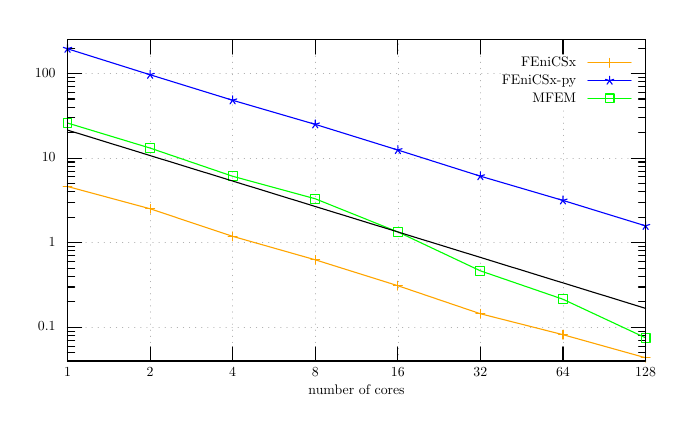
\begin{tikzpicture}[gnuplot]
%% generated with GNUPLOT 6.0p1 (Lua 5.4; terminal rev. Jun 2020, script rev. 118)
%% ven. 10 janv. 2025 17:58:53
\tikzset{every node/.append style={scale=0.50}}
\path (0.000,0.000) rectangle (8.125,4.725);
\gpcolor{color=gp lt color border}
\gpsetlinetype{gp lt border}
\gpsetdashtype{gp dt solid}
\gpsetlinewidth{1.00}
\draw[gp path] (0.506,0.492)--(0.596,0.492);
\draw[gp path] (7.848,0.492)--(7.758,0.492);
\draw[gp path] (0.506,0.596)--(0.596,0.596);
\draw[gp path] (7.848,0.596)--(7.758,0.596);
\draw[gp path] (0.506,0.681)--(0.596,0.681);
\draw[gp path] (7.848,0.681)--(7.758,0.681);
\draw[gp path] (0.506,0.753)--(0.596,0.753);
\draw[gp path] (7.848,0.753)--(7.758,0.753);
\draw[gp path] (0.506,0.815)--(0.596,0.815);
\draw[gp path] (7.848,0.815)--(7.758,0.815);
\draw[gp path] (0.506,0.870)--(0.596,0.870);
\draw[gp path] (7.848,0.870)--(7.758,0.870);
\gpcolor{color=gp lt color axes}
\gpsetlinetype{gp lt axes}
\gpsetdashtype{gp dt axes}
\gpsetlinewidth{0.50}
\draw[gp path] (0.506,0.920)--(7.848,0.920);
\gpcolor{color=gp lt color border}
\gpsetlinetype{gp lt border}
\gpsetdashtype{gp dt solid}
\gpsetlinewidth{1.00}
\draw[gp path] (0.506,0.920)--(0.686,0.920);
\draw[gp path] (7.848,0.920)--(7.668,0.920);
\node[gp node right] at (0.414,0.920) {$0.1$};
\draw[gp path] (0.506,1.243)--(0.596,1.243);
\draw[gp path] (7.848,1.243)--(7.758,1.243);
\draw[gp path] (0.506,1.432)--(0.596,1.432);
\draw[gp path] (7.848,1.432)--(7.758,1.432);
\draw[gp path] (0.506,1.566)--(0.596,1.566);
\draw[gp path] (7.848,1.566)--(7.758,1.566);
\draw[gp path] (0.506,1.670)--(0.596,1.670);
\draw[gp path] (7.848,1.670)--(7.758,1.670);
\draw[gp path] (0.506,1.756)--(0.596,1.756);
\draw[gp path] (7.848,1.756)--(7.758,1.756);
\draw[gp path] (0.506,1.827)--(0.596,1.827);
\draw[gp path] (7.848,1.827)--(7.758,1.827);
\draw[gp path] (0.506,1.890)--(0.596,1.890);
\draw[gp path] (7.848,1.890)--(7.758,1.890);
\draw[gp path] (0.506,1.945)--(0.596,1.945);
\draw[gp path] (7.848,1.945)--(7.758,1.945);
\gpcolor{color=gp lt color axes}
\gpsetlinetype{gp lt axes}
\gpsetdashtype{gp dt axes}
\gpsetlinewidth{0.50}
\draw[gp path] (0.506,1.994)--(7.848,1.994);
\gpcolor{color=gp lt color border}
\gpsetlinetype{gp lt border}
\gpsetdashtype{gp dt solid}
\gpsetlinewidth{1.00}
\draw[gp path] (0.506,1.994)--(0.686,1.994);
\draw[gp path] (7.848,1.994)--(7.668,1.994);
\node[gp node right] at (0.414,1.994) {$1$};
\draw[gp path] (0.506,2.317)--(0.596,2.317);
\draw[gp path] (7.848,2.317)--(7.758,2.317);
\draw[gp path] (0.506,2.506)--(0.596,2.506);
\draw[gp path] (7.848,2.506)--(7.758,2.506);
\draw[gp path] (0.506,2.641)--(0.596,2.641);
\draw[gp path] (7.848,2.641)--(7.758,2.641);
\draw[gp path] (0.506,2.745)--(0.596,2.745);
\draw[gp path] (7.848,2.745)--(7.758,2.745);
\draw[gp path] (0.506,2.830)--(0.596,2.830);
\draw[gp path] (7.848,2.830)--(7.758,2.830);
\draw[gp path] (0.506,2.902)--(0.596,2.902);
\draw[gp path] (7.848,2.902)--(7.758,2.902);
\draw[gp path] (0.506,2.964)--(0.596,2.964);
\draw[gp path] (7.848,2.964)--(7.758,2.964);
\draw[gp path] (0.506,3.019)--(0.596,3.019);
\draw[gp path] (7.848,3.019)--(7.758,3.019);
\gpcolor{color=gp lt color axes}
\gpsetlinetype{gp lt axes}
\gpsetdashtype{gp dt axes}
\gpsetlinewidth{0.50}
\draw[gp path] (0.506,3.068)--(7.848,3.068);
\gpcolor{color=gp lt color border}
\gpsetlinetype{gp lt border}
\gpsetdashtype{gp dt solid}
\gpsetlinewidth{1.00}
\draw[gp path] (0.506,3.068)--(0.686,3.068);
\draw[gp path] (7.848,3.068)--(7.668,3.068);
\node[gp node right] at (0.414,3.068) {$10$};
\draw[gp path] (0.506,3.392)--(0.596,3.392);
\draw[gp path] (7.848,3.392)--(7.758,3.392);
\draw[gp path] (0.506,3.581)--(0.596,3.581);
\draw[gp path] (7.848,3.581)--(7.758,3.581);
\draw[gp path] (0.506,3.715)--(0.596,3.715);
\draw[gp path] (7.848,3.715)--(7.758,3.715);
\draw[gp path] (0.506,3.819)--(0.596,3.819);
\draw[gp path] (7.848,3.819)--(7.758,3.819);
\draw[gp path] (0.506,3.904)--(0.596,3.904);
\draw[gp path] (7.848,3.904)--(7.758,3.904);
\draw[gp path] (0.506,3.976)--(0.596,3.976);
\draw[gp path] (7.848,3.976)--(7.758,3.976);
\draw[gp path] (0.506,4.038)--(0.596,4.038);
\draw[gp path] (7.848,4.038)--(7.758,4.038);
\draw[gp path] (0.506,4.093)--(0.596,4.093);
\draw[gp path] (7.848,4.093)--(7.758,4.093);
\gpcolor{color=gp lt color axes}
\gpsetlinetype{gp lt axes}
\gpsetdashtype{gp dt axes}
\gpsetlinewidth{0.50}
\draw[gp path] (0.506,4.142)--(6.104,4.142);
\draw[gp path] (7.756,4.142)--(7.848,4.142);
\gpcolor{color=gp lt color border}
\gpsetlinetype{gp lt border}
\gpsetdashtype{gp dt solid}
\gpsetlinewidth{1.00}
\draw[gp path] (0.506,4.142)--(0.686,4.142);
\draw[gp path] (7.848,4.142)--(7.668,4.142);
\node[gp node right] at (0.414,4.142) {$100$};
\draw[gp path] (0.506,4.466)--(0.596,4.466);
\draw[gp path] (7.848,4.466)--(7.758,4.466);
\gpcolor{color=gp lt color axes}
\gpsetlinetype{gp lt axes}
\gpsetdashtype{gp dt axes}
\gpsetlinewidth{0.50}
\draw[gp path] (0.506,0.492)--(0.506,4.570);
\gpcolor{color=gp lt color border}
\gpsetlinetype{gp lt border}
\gpsetdashtype{gp dt solid}
\gpsetlinewidth{1.00}
\draw[gp path] (0.506,0.492)--(0.506,0.672);
\draw[gp path] (0.506,4.570)--(0.506,4.390);
\node[gp node center] at (0.506,0.338) {1};
\gpcolor{color=gp lt color axes}
\gpsetlinetype{gp lt axes}
\gpsetdashtype{gp dt axes}
\gpsetlinewidth{0.50}
\draw[gp path] (1.555,0.492)--(1.555,4.570);
\gpcolor{color=gp lt color border}
\gpsetlinetype{gp lt border}
\gpsetdashtype{gp dt solid}
\gpsetlinewidth{1.00}
\draw[gp path] (1.555,0.492)--(1.555,0.672);
\draw[gp path] (1.555,4.570)--(1.555,4.390);
\node[gp node center] at (1.555,0.338) {2};
\gpcolor{color=gp lt color axes}
\gpsetlinetype{gp lt axes}
\gpsetdashtype{gp dt axes}
\gpsetlinewidth{0.50}
\draw[gp path] (2.603,0.492)--(2.603,4.570);
\gpcolor{color=gp lt color border}
\gpsetlinetype{gp lt border}
\gpsetdashtype{gp dt solid}
\gpsetlinewidth{1.00}
\draw[gp path] (2.603,0.492)--(2.603,0.672);
\draw[gp path] (2.603,4.570)--(2.603,4.390);
\node[gp node center] at (2.603,0.338) {4};
\gpcolor{color=gp lt color axes}
\gpsetlinetype{gp lt axes}
\gpsetdashtype{gp dt axes}
\gpsetlinewidth{0.50}
\draw[gp path] (3.652,0.492)--(3.652,4.570);
\gpcolor{color=gp lt color border}
\gpsetlinetype{gp lt border}
\gpsetdashtype{gp dt solid}
\gpsetlinewidth{1.00}
\draw[gp path] (3.652,0.492)--(3.652,0.672);
\draw[gp path] (3.652,4.570)--(3.652,4.390);
\node[gp node center] at (3.652,0.338) {8};
\gpcolor{color=gp lt color axes}
\gpsetlinetype{gp lt axes}
\gpsetdashtype{gp dt axes}
\gpsetlinewidth{0.50}
\draw[gp path] (4.701,0.492)--(4.701,4.570);
\gpcolor{color=gp lt color border}
\gpsetlinetype{gp lt border}
\gpsetdashtype{gp dt solid}
\gpsetlinewidth{1.00}
\draw[gp path] (4.701,0.492)--(4.701,0.672);
\draw[gp path] (4.701,4.570)--(4.701,4.390);
\node[gp node center] at (4.701,0.338) {16};
\gpcolor{color=gp lt color axes}
\gpsetlinetype{gp lt axes}
\gpsetdashtype{gp dt axes}
\gpsetlinewidth{0.50}
\draw[gp path] (5.749,0.492)--(5.749,4.570);
\gpcolor{color=gp lt color border}
\gpsetlinetype{gp lt border}
\gpsetdashtype{gp dt solid}
\gpsetlinewidth{1.00}
\draw[gp path] (5.749,0.492)--(5.749,0.672);
\draw[gp path] (5.749,4.570)--(5.749,4.390);
\node[gp node center] at (5.749,0.338) {32};
\gpcolor{color=gp lt color axes}
\gpsetlinetype{gp lt axes}
\gpsetdashtype{gp dt axes}
\gpsetlinewidth{0.50}
\draw[gp path] (6.798,0.492)--(6.798,3.715);
\draw[gp path] (6.798,4.390)--(6.798,4.570);
\gpcolor{color=gp lt color border}
\gpsetlinetype{gp lt border}
\gpsetdashtype{gp dt solid}
\gpsetlinewidth{1.00}
\draw[gp path] (6.798,0.492)--(6.798,0.672);
\draw[gp path] (6.798,4.570)--(6.798,4.390);
\node[gp node center] at (6.798,0.338) {64};
\gpcolor{color=gp lt color axes}
\gpsetlinetype{gp lt axes}
\gpsetdashtype{gp dt axes}
\gpsetlinewidth{0.50}
\draw[gp path] (7.847,0.492)--(7.847,4.570);
\gpcolor{color=gp lt color border}
\gpsetlinetype{gp lt border}
\gpsetdashtype{gp dt solid}
\gpsetlinewidth{1.00}
\draw[gp path] (7.847,0.492)--(7.847,0.672);
\draw[gp path] (7.847,4.570)--(7.847,4.390);
\node[gp node center] at (7.847,0.338) {128};
\draw[gp path] (0.506,4.570)--(0.506,0.492)--(7.848,0.492)--(7.848,4.570)--cycle;
\node[gp node right] at (7.024,4.277) {FEniCSx};
\gpcolor{rgb color={1.000,0.647,0.000}}
\draw[gp path] (7.116,4.277)--(7.664,4.277);
\draw[gp path] (0.506,2.708)--(1.555,2.425)--(2.603,2.075)--(3.652,1.777)--(4.701,1.448)%
  --(5.749,1.092)--(6.798,0.826)--(7.847,0.533);
\gpsetpointsize{4.00}
\gp3point{gp mark 1}{}{(0.506,2.708)}
\gp3point{gp mark 1}{}{(1.555,2.425)}
\gp3point{gp mark 1}{}{(2.603,2.075)}
\gp3point{gp mark 1}{}{(3.652,1.777)}
\gp3point{gp mark 1}{}{(4.701,1.448)}
\gp3point{gp mark 1}{}{(5.749,1.092)}
\gp3point{gp mark 1}{}{(6.798,0.826)}
\gp3point{gp mark 1}{}{(7.847,0.533)}
\gp3point{gp mark 1}{}{(7.390,4.277)}
\gpcolor{color=gp lt color border}
\node[gp node right] at (7.024,4.052) {FEniCSx-py};
\gpcolor{rgb color={0.000,0.000,1.000}}
\draw[gp path] (7.116,4.052)--(7.664,4.052);
\draw[gp path] (0.506,4.457)--(1.555,4.127)--(2.603,3.803)--(3.652,3.497)--(4.701,3.171)%
  --(5.749,2.839)--(6.798,2.531)--(7.847,2.208);
\gp3point{gp mark 3}{}{(0.506,4.457)}
\gp3point{gp mark 3}{}{(1.555,4.127)}
\gp3point{gp mark 3}{}{(2.603,3.803)}
\gp3point{gp mark 3}{}{(3.652,3.497)}
\gp3point{gp mark 3}{}{(4.701,3.171)}
\gp3point{gp mark 3}{}{(5.749,2.839)}
\gp3point{gp mark 3}{}{(6.798,2.531)}
\gp3point{gp mark 3}{}{(7.847,2.208)}
\gp3point{gp mark 3}{}{(7.390,4.052)}
\gpcolor{color=gp lt color border}
\node[gp node right] at (7.024,3.827) {MFEM};
\gpcolor{rgb color={0.000,1.000,0.000}}
\draw[gp path] (7.116,3.827)--(7.664,3.827);
\draw[gp path] (0.506,3.514)--(1.555,3.196)--(2.603,2.838)--(3.652,2.552)--(4.701,2.131)%
  --(5.749,1.637)--(6.798,1.276)--(7.847,0.786);
\gp3point{gp mark 4}{}{(0.506,3.514)}
\gp3point{gp mark 4}{}{(1.555,3.196)}
\gp3point{gp mark 4}{}{(2.603,2.838)}
\gp3point{gp mark 4}{}{(3.652,2.552)}
\gp3point{gp mark 4}{}{(4.701,2.131)}
\gp3point{gp mark 4}{}{(5.749,1.637)}
\gp3point{gp mark 4}{}{(6.798,1.276)}
\gp3point{gp mark 4}{}{(7.847,0.786)}
\gp3point{gp mark 4}{}{(7.390,3.827)}
\gpcolor{rgb color={0.000,0.000,0.000}}
\draw[gp path] (0.506,3.424)--(0.580,3.401)--(0.654,3.379)--(0.728,3.356)--(0.803,3.333)%
  --(0.877,3.310)--(0.951,3.287)--(1.025,3.264)--(1.099,3.241)--(1.173,3.219)--(1.247,3.196)%
  --(1.322,3.173)--(1.396,3.150)--(1.470,3.127)--(1.544,3.104)--(1.618,3.081)--(1.692,3.058)%
  --(1.767,3.036)--(1.841,3.013)--(1.915,2.990)--(1.989,2.967)--(2.063,2.944)--(2.137,2.921)%
  --(2.211,2.898)--(2.286,2.876)--(2.360,2.853)--(2.434,2.830)--(2.508,2.807)--(2.582,2.784)%
  --(2.656,2.761)--(2.730,2.738)--(2.805,2.715)--(2.879,2.693)--(2.953,2.670)--(3.027,2.647)%
  --(3.101,2.624)--(3.175,2.601)--(3.250,2.578)--(3.324,2.555)--(3.398,2.533)--(3.472,2.510)%
  --(3.546,2.487)--(3.620,2.464)--(3.694,2.441)--(3.769,2.418)--(3.843,2.395)--(3.917,2.372)%
  --(3.991,2.350)--(4.065,2.327)--(4.139,2.304)--(4.213,2.281)--(4.288,2.258)--(4.362,2.235)%
  --(4.436,2.212)--(4.510,2.190)--(4.584,2.167)--(4.658,2.144)--(4.733,2.121)--(4.807,2.098)%
  --(4.881,2.075)--(4.955,2.052)--(5.029,2.029)--(5.103,2.007)--(5.177,1.984)--(5.252,1.961)%
  --(5.326,1.938)--(5.400,1.915)--(5.474,1.892)--(5.548,1.869)--(5.622,1.847)--(5.696,1.824)%
  --(5.771,1.801)--(5.845,1.778)--(5.919,1.755)--(5.993,1.732)--(6.067,1.709)--(6.141,1.686)%
  --(6.216,1.664)--(6.290,1.641)--(6.364,1.618)--(6.438,1.595)--(6.512,1.572)--(6.586,1.549)%
  --(6.660,1.526)--(6.735,1.503)--(6.809,1.481)--(6.883,1.458)--(6.957,1.435)--(7.031,1.412)%
  --(7.105,1.389)--(7.179,1.366)--(7.254,1.343)--(7.328,1.321)--(7.402,1.298)--(7.476,1.275)%
  --(7.550,1.252)--(7.624,1.229)--(7.699,1.206)--(7.773,1.183)--(7.847,1.160);
\gpcolor{color=gp lt color border}
\draw[gp path] (0.506,4.570)--(0.506,0.492)--(7.848,0.492)--(7.848,4.570)--cycle;
\node[gp node center] at (4.177,0.107) {number of cores};
%% coordinates of the plot area
\gpdefrectangularnode{gp plot 1}{\pgfpoint{0.506cm}{0.492cm}}{\pgfpoint{7.848cm}{4.570cm}}
\end{tikzpicture}
%% gnuplot variables

		\label{time_dam}}
	\subfloat[Damage generation (Ratio vs MFEM)]{
		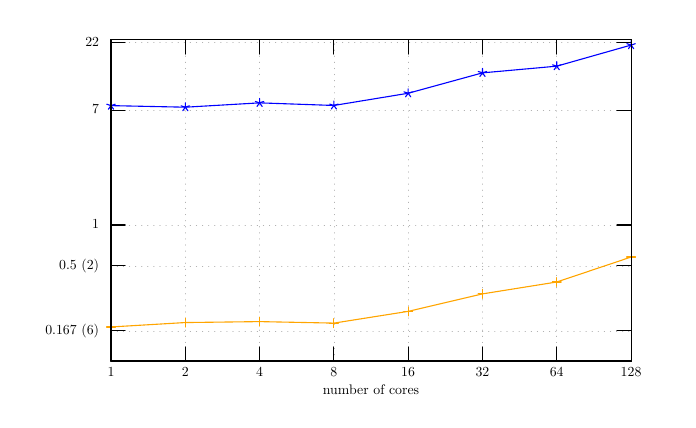
\begin{tikzpicture}[gnuplot]
%% generated with GNUPLOT 6.0p1 (Lua 5.4; terminal rev. Jun 2020, script rev. 118)
%% ven. 10 janv. 2025 17:58:53
\tikzset{every node/.append style={scale=0.50}}
\path (0.000,0.000) rectangle (8.125,4.725);
\gpcolor{color=gp lt color axes}
\gpsetlinetype{gp lt axes}
\gpsetdashtype{gp dt axes}
\gpsetlinewidth{0.50}
\draw[gp path] (1.058,0.875)--(7.664,0.875);
\gpcolor{color=gp lt color border}
\gpsetlinetype{gp lt border}
\gpsetdashtype{gp dt solid}
\gpsetlinewidth{1.00}
\draw[gp path] (1.058,0.875)--(1.238,0.875);
\draw[gp path] (7.664,0.875)--(7.484,0.875);
\node[gp node right] at (0.966,0.875) {0.167 (6)};
\gpcolor{color=gp lt color axes}
\gpsetlinetype{gp lt axes}
\gpsetdashtype{gp dt axes}
\gpsetlinewidth{0.50}
\draw[gp path] (1.058,1.699)--(7.664,1.699);
\gpcolor{color=gp lt color border}
\gpsetlinetype{gp lt border}
\gpsetdashtype{gp dt solid}
\gpsetlinewidth{1.00}
\draw[gp path] (1.058,1.699)--(1.238,1.699);
\draw[gp path] (7.664,1.699)--(7.484,1.699);
\node[gp node right] at (0.966,1.699) {0.5 (2)};
\gpcolor{color=gp lt color axes}
\gpsetlinetype{gp lt axes}
\gpsetdashtype{gp dt axes}
\gpsetlinewidth{0.50}
\draw[gp path] (1.058,2.219)--(7.664,2.219);
\gpcolor{color=gp lt color border}
\gpsetlinetype{gp lt border}
\gpsetdashtype{gp dt solid}
\gpsetlinewidth{1.00}
\draw[gp path] (1.058,2.219)--(1.238,2.219);
\draw[gp path] (7.664,2.219)--(7.484,2.219);
\node[gp node right] at (0.966,2.219) {$1$};
\gpcolor{color=gp lt color axes}
\gpsetlinetype{gp lt axes}
\gpsetdashtype{gp dt axes}
\gpsetlinewidth{0.50}
\draw[gp path] (1.058,3.678)--(7.664,3.678);
\gpcolor{color=gp lt color border}
\gpsetlinetype{gp lt border}
\gpsetdashtype{gp dt solid}
\gpsetlinewidth{1.00}
\draw[gp path] (1.058,3.678)--(1.238,3.678);
\draw[gp path] (7.664,3.678)--(7.484,3.678);
\node[gp node right] at (0.966,3.678) {$7$};
\gpcolor{color=gp lt color axes}
\gpsetlinetype{gp lt axes}
\gpsetdashtype{gp dt axes}
\gpsetlinewidth{0.50}
\draw[gp path] (1.058,4.537)--(7.664,4.537);
\gpcolor{color=gp lt color border}
\gpsetlinetype{gp lt border}
\gpsetdashtype{gp dt solid}
\gpsetlinewidth{1.00}
\draw[gp path] (1.058,4.537)--(1.238,4.537);
\draw[gp path] (7.664,4.537)--(7.484,4.537);
\node[gp node right] at (0.966,4.537) {$22$};
\gpcolor{color=gp lt color axes}
\gpsetlinetype{gp lt axes}
\gpsetdashtype{gp dt axes}
\gpsetlinewidth{0.50}
\draw[gp path] (1.058,0.492)--(1.058,4.570);
\gpcolor{color=gp lt color border}
\gpsetlinetype{gp lt border}
\gpsetdashtype{gp dt solid}
\gpsetlinewidth{1.00}
\draw[gp path] (1.058,0.492)--(1.058,0.672);
\draw[gp path] (1.058,4.570)--(1.058,4.390);
\node[gp node center] at (1.058,0.338) {1};
\gpcolor{color=gp lt color axes}
\gpsetlinetype{gp lt axes}
\gpsetdashtype{gp dt axes}
\gpsetlinewidth{0.50}
\draw[gp path] (2.002,0.492)--(2.002,4.570);
\gpcolor{color=gp lt color border}
\gpsetlinetype{gp lt border}
\gpsetdashtype{gp dt solid}
\gpsetlinewidth{1.00}
\draw[gp path] (2.002,0.492)--(2.002,0.672);
\draw[gp path] (2.002,4.570)--(2.002,4.390);
\node[gp node center] at (2.002,0.338) {2};
\gpcolor{color=gp lt color axes}
\gpsetlinetype{gp lt axes}
\gpsetdashtype{gp dt axes}
\gpsetlinewidth{0.50}
\draw[gp path] (2.945,0.492)--(2.945,4.570);
\gpcolor{color=gp lt color border}
\gpsetlinetype{gp lt border}
\gpsetdashtype{gp dt solid}
\gpsetlinewidth{1.00}
\draw[gp path] (2.945,0.492)--(2.945,0.672);
\draw[gp path] (2.945,4.570)--(2.945,4.390);
\node[gp node center] at (2.945,0.338) {4};
\gpcolor{color=gp lt color axes}
\gpsetlinetype{gp lt axes}
\gpsetdashtype{gp dt axes}
\gpsetlinewidth{0.50}
\draw[gp path] (3.889,0.492)--(3.889,4.570);
\gpcolor{color=gp lt color border}
\gpsetlinetype{gp lt border}
\gpsetdashtype{gp dt solid}
\gpsetlinewidth{1.00}
\draw[gp path] (3.889,0.492)--(3.889,0.672);
\draw[gp path] (3.889,4.570)--(3.889,4.390);
\node[gp node center] at (3.889,0.338) {8};
\gpcolor{color=gp lt color axes}
\gpsetlinetype{gp lt axes}
\gpsetdashtype{gp dt axes}
\gpsetlinewidth{0.50}
\draw[gp path] (4.832,0.492)--(4.832,4.570);
\gpcolor{color=gp lt color border}
\gpsetlinetype{gp lt border}
\gpsetdashtype{gp dt solid}
\gpsetlinewidth{1.00}
\draw[gp path] (4.832,0.492)--(4.832,0.672);
\draw[gp path] (4.832,4.570)--(4.832,4.390);
\node[gp node center] at (4.832,0.338) {16};
\gpcolor{color=gp lt color axes}
\gpsetlinetype{gp lt axes}
\gpsetdashtype{gp dt axes}
\gpsetlinewidth{0.50}
\draw[gp path] (5.776,0.492)--(5.776,4.570);
\gpcolor{color=gp lt color border}
\gpsetlinetype{gp lt border}
\gpsetdashtype{gp dt solid}
\gpsetlinewidth{1.00}
\draw[gp path] (5.776,0.492)--(5.776,0.672);
\draw[gp path] (5.776,4.570)--(5.776,4.390);
\node[gp node center] at (5.776,0.338) {32};
\gpcolor{color=gp lt color axes}
\gpsetlinetype{gp lt axes}
\gpsetdashtype{gp dt axes}
\gpsetlinewidth{0.50}
\draw[gp path] (6.719,0.492)--(6.719,4.570);
\gpcolor{color=gp lt color border}
\gpsetlinetype{gp lt border}
\gpsetdashtype{gp dt solid}
\gpsetlinewidth{1.00}
\draw[gp path] (6.719,0.492)--(6.719,0.672);
\draw[gp path] (6.719,4.570)--(6.719,4.390);
\node[gp node center] at (6.719,0.338) {64};
\gpcolor{color=gp lt color axes}
\gpsetlinetype{gp lt axes}
\gpsetdashtype{gp dt axes}
\gpsetlinewidth{0.50}
\draw[gp path] (7.663,0.492)--(7.663,4.570);
\gpcolor{color=gp lt color border}
\gpsetlinetype{gp lt border}
\gpsetdashtype{gp dt solid}
\gpsetlinewidth{1.00}
\draw[gp path] (7.663,0.492)--(7.663,0.672);
\draw[gp path] (7.663,4.570)--(7.663,4.390);
\node[gp node center] at (7.663,0.338) {128};
\draw[gp path] (1.058,4.570)--(1.058,0.492)--(7.664,0.492)--(7.664,4.570)--cycle;
\gpcolor{rgb color={1.000,0.647,0.000}}
\draw[gp path] (1.058,0.924)--(2.002,0.980)--(2.945,0.992)--(3.889,0.973)--(4.832,1.122)%
  --(5.776,1.344)--(6.719,1.495)--(7.663,1.812);
\gpsetpointsize{4.00}
\gp3point{gp mark 1}{}{(1.058,0.924)}
\gp3point{gp mark 1}{}{(2.002,0.980)}
\gp3point{gp mark 1}{}{(2.945,0.992)}
\gp3point{gp mark 1}{}{(3.889,0.973)}
\gp3point{gp mark 1}{}{(4.832,1.122)}
\gp3point{gp mark 1}{}{(5.776,1.344)}
\gp3point{gp mark 1}{}{(6.719,1.495)}
\gp3point{gp mark 1}{}{(7.663,1.812)}
\gpcolor{rgb color={0.000,0.000,1.000}}
\draw[gp path] (1.058,3.735)--(2.002,3.715)--(2.945,3.770)--(3.889,3.737)--(4.832,3.892)%
  --(5.776,4.151)--(6.719,4.236)--(7.663,4.504);
\gp3point{gp mark 3}{}{(1.058,3.735)}
\gp3point{gp mark 3}{}{(2.002,3.715)}
\gp3point{gp mark 3}{}{(2.945,3.770)}
\gp3point{gp mark 3}{}{(3.889,3.737)}
\gp3point{gp mark 3}{}{(4.832,3.892)}
\gp3point{gp mark 3}{}{(5.776,4.151)}
\gp3point{gp mark 3}{}{(6.719,4.236)}
\gp3point{gp mark 3}{}{(7.663,4.504)}
\gpcolor{color=gp lt color border}
\draw[gp path] (1.058,4.570)--(1.058,0.492)--(7.664,0.492)--(7.664,4.570)--cycle;
\node[gp node center] at (4.361,0.107) {number of cores};
%% coordinates of the plot area
\gpdefrectangularnode{gp plot 1}{\pgfpoint{1.058cm}{0.492cm}}{\pgfpoint{7.664cm}{4.570cm}}
\end{tikzpicture}
%% gnuplot variables

		\label{time_dam_r}}
	\caption{Elapsed time function of the number of processes: Simulation, mesh and damage creation (in log-log scale except for y axes of \protect\subref*{time_simu_r}  )\label{elapsed1}}
\end{figure}
\begin{figure}
	\subfloat[Elementary vector creation (in s)]{
		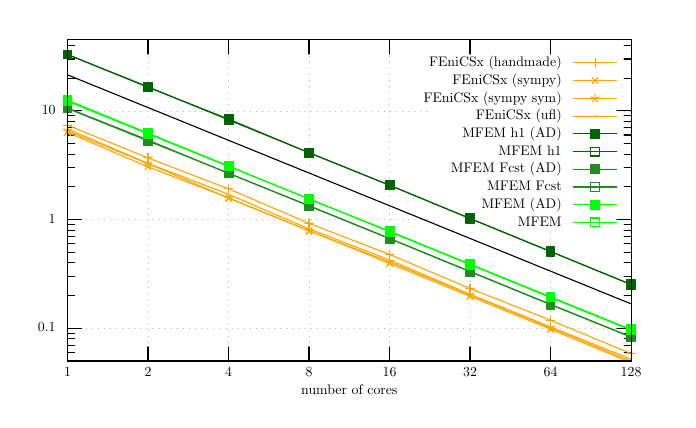
\begin{tikzpicture}[gnuplot]
%% generated with GNUPLOT 6.0p1 (Lua 5.4; terminal rev. Jun 2020, script rev. 118)
%% ven. 10 janv. 2025 17:58:53
\tikzset{every node/.append style={scale=0.50}}
\path (0.000,0.000) rectangle (8.125,4.725);
\gpcolor{color=gp lt color border}
\gpsetlinetype{gp lt border}
\gpsetdashtype{gp dt solid}
\gpsetlinewidth{1.00}
\draw[gp path] (0.506,0.492)--(0.596,0.492);
\draw[gp path] (7.664,0.492)--(7.574,0.492);
\draw[gp path] (0.506,0.601)--(0.596,0.601);
\draw[gp path] (7.664,0.601)--(7.574,0.601);
\draw[gp path] (0.506,0.694)--(0.596,0.694);
\draw[gp path] (7.664,0.694)--(7.574,0.694);
\draw[gp path] (0.506,0.774)--(0.596,0.774);
\draw[gp path] (7.664,0.774)--(7.574,0.774);
\draw[gp path] (0.506,0.844)--(0.596,0.844);
\draw[gp path] (7.664,0.844)--(7.574,0.844);
\gpcolor{color=gp lt color axes}
\gpsetlinetype{gp lt axes}
\gpsetdashtype{gp dt axes}
\gpsetlinewidth{0.50}
\draw[gp path] (0.506,0.908)--(7.664,0.908);
\gpcolor{color=gp lt color border}
\gpsetlinetype{gp lt border}
\gpsetdashtype{gp dt solid}
\gpsetlinewidth{1.00}
\draw[gp path] (0.506,0.908)--(0.686,0.908);
\draw[gp path] (7.664,0.908)--(7.484,0.908);
\node[gp node right] at (0.414,0.908) {$0.1$};
\draw[gp path] (0.506,1.323)--(0.596,1.323);
\draw[gp path] (7.664,1.323)--(7.574,1.323);
\draw[gp path] (0.506,1.566)--(0.596,1.566);
\draw[gp path] (7.664,1.566)--(7.574,1.566);
\draw[gp path] (0.506,1.739)--(0.596,1.739);
\draw[gp path] (7.664,1.739)--(7.574,1.739);
\draw[gp path] (0.506,1.872)--(0.596,1.872);
\draw[gp path] (7.664,1.872)--(7.574,1.872);
\draw[gp path] (0.506,1.982)--(0.596,1.982);
\draw[gp path] (7.664,1.982)--(7.574,1.982);
\draw[gp path] (0.506,2.074)--(0.596,2.074);
\draw[gp path] (7.664,2.074)--(7.574,2.074);
\draw[gp path] (0.506,2.154)--(0.596,2.154);
\draw[gp path] (7.664,2.154)--(7.574,2.154);
\draw[gp path] (0.506,2.225)--(0.596,2.225);
\draw[gp path] (7.664,2.225)--(7.574,2.225);
\gpcolor{color=gp lt color axes}
\gpsetlinetype{gp lt axes}
\gpsetdashtype{gp dt axes}
\gpsetlinewidth{0.50}
\draw[gp path] (0.506,2.288)--(5.092,2.288);
\draw[gp path] (7.572,2.288)--(7.664,2.288);
\gpcolor{color=gp lt color border}
\gpsetlinetype{gp lt border}
\gpsetdashtype{gp dt solid}
\gpsetlinewidth{1.00}
\draw[gp path] (0.506,2.288)--(0.686,2.288);
\draw[gp path] (7.664,2.288)--(7.484,2.288);
\node[gp node right] at (0.414,2.288) {$1$};
\draw[gp path] (0.506,2.703)--(0.596,2.703);
\draw[gp path] (7.664,2.703)--(7.574,2.703);
\draw[gp path] (0.506,2.947)--(0.596,2.947);
\draw[gp path] (7.664,2.947)--(7.574,2.947);
\draw[gp path] (0.506,3.119)--(0.596,3.119);
\draw[gp path] (7.664,3.119)--(7.574,3.119);
\draw[gp path] (0.506,3.253)--(0.596,3.253);
\draw[gp path] (7.664,3.253)--(7.574,3.253);
\draw[gp path] (0.506,3.362)--(0.596,3.362);
\draw[gp path] (7.664,3.362)--(7.574,3.362);
\draw[gp path] (0.506,3.454)--(0.596,3.454);
\draw[gp path] (7.664,3.454)--(7.574,3.454);
\draw[gp path] (0.506,3.535)--(0.596,3.535);
\draw[gp path] (7.664,3.535)--(7.574,3.535);
\draw[gp path] (0.506,3.605)--(0.596,3.605);
\draw[gp path] (7.664,3.605)--(7.574,3.605);
\gpcolor{color=gp lt color axes}
\gpsetlinetype{gp lt axes}
\gpsetdashtype{gp dt axes}
\gpsetlinewidth{0.50}
\draw[gp path] (0.506,3.668)--(5.092,3.668);
\draw[gp path] (7.572,3.668)--(7.664,3.668);
\gpcolor{color=gp lt color border}
\gpsetlinetype{gp lt border}
\gpsetdashtype{gp dt solid}
\gpsetlinewidth{1.00}
\draw[gp path] (0.506,3.668)--(0.686,3.668);
\draw[gp path] (7.664,3.668)--(7.484,3.668);
\node[gp node right] at (0.414,3.668) {$10$};
\draw[gp path] (0.506,4.084)--(0.596,4.084);
\draw[gp path] (7.664,4.084)--(7.574,4.084);
\draw[gp path] (0.506,4.327)--(0.596,4.327);
\draw[gp path] (7.664,4.327)--(7.574,4.327);
\draw[gp path] (0.506,4.499)--(0.596,4.499);
\draw[gp path] (7.664,4.499)--(7.574,4.499);
\gpcolor{color=gp lt color axes}
\gpsetlinetype{gp lt axes}
\gpsetdashtype{gp dt axes}
\gpsetlinewidth{0.50}
\draw[gp path] (0.506,0.492)--(0.506,4.570);
\gpcolor{color=gp lt color border}
\gpsetlinetype{gp lt border}
\gpsetdashtype{gp dt solid}
\gpsetlinewidth{1.00}
\draw[gp path] (0.506,0.492)--(0.506,0.672);
\draw[gp path] (0.506,4.570)--(0.506,4.390);
\node[gp node center] at (0.506,0.338) {1};
\gpcolor{color=gp lt color axes}
\gpsetlinetype{gp lt axes}
\gpsetdashtype{gp dt axes}
\gpsetlinewidth{0.50}
\draw[gp path] (1.528,0.492)--(1.528,4.570);
\gpcolor{color=gp lt color border}
\gpsetlinetype{gp lt border}
\gpsetdashtype{gp dt solid}
\gpsetlinewidth{1.00}
\draw[gp path] (1.528,0.492)--(1.528,0.672);
\draw[gp path] (1.528,4.570)--(1.528,4.390);
\node[gp node center] at (1.528,0.338) {2};
\gpcolor{color=gp lt color axes}
\gpsetlinetype{gp lt axes}
\gpsetdashtype{gp dt axes}
\gpsetlinewidth{0.50}
\draw[gp path] (2.551,0.492)--(2.551,4.570);
\gpcolor{color=gp lt color border}
\gpsetlinetype{gp lt border}
\gpsetdashtype{gp dt solid}
\gpsetlinewidth{1.00}
\draw[gp path] (2.551,0.492)--(2.551,0.672);
\draw[gp path] (2.551,4.570)--(2.551,4.390);
\node[gp node center] at (2.551,0.338) {4};
\gpcolor{color=gp lt color axes}
\gpsetlinetype{gp lt axes}
\gpsetdashtype{gp dt axes}
\gpsetlinewidth{0.50}
\draw[gp path] (3.573,0.492)--(3.573,4.570);
\gpcolor{color=gp lt color border}
\gpsetlinetype{gp lt border}
\gpsetdashtype{gp dt solid}
\gpsetlinewidth{1.00}
\draw[gp path] (3.573,0.492)--(3.573,0.672);
\draw[gp path] (3.573,4.570)--(3.573,4.390);
\node[gp node center] at (3.573,0.338) {8};
\gpcolor{color=gp lt color axes}
\gpsetlinetype{gp lt axes}
\gpsetdashtype{gp dt axes}
\gpsetlinewidth{0.50}
\draw[gp path] (4.596,0.492)--(4.596,4.570);
\gpcolor{color=gp lt color border}
\gpsetlinetype{gp lt border}
\gpsetdashtype{gp dt solid}
\gpsetlinewidth{1.00}
\draw[gp path] (4.596,0.492)--(4.596,0.672);
\draw[gp path] (4.596,4.570)--(4.596,4.390);
\node[gp node center] at (4.596,0.338) {16};
\gpcolor{color=gp lt color axes}
\gpsetlinetype{gp lt axes}
\gpsetdashtype{gp dt axes}
\gpsetlinewidth{0.50}
\draw[gp path] (5.618,0.492)--(5.618,2.140);
\draw[gp path] (5.618,4.390)--(5.618,4.570);
\gpcolor{color=gp lt color border}
\gpsetlinetype{gp lt border}
\gpsetdashtype{gp dt solid}
\gpsetlinewidth{1.00}
\draw[gp path] (5.618,0.492)--(5.618,0.672);
\draw[gp path] (5.618,4.570)--(5.618,4.390);
\node[gp node center] at (5.618,0.338) {32};
\gpcolor{color=gp lt color axes}
\gpsetlinetype{gp lt axes}
\gpsetdashtype{gp dt axes}
\gpsetlinewidth{0.50}
\draw[gp path] (6.640,0.492)--(6.640,2.140);
\draw[gp path] (6.640,4.390)--(6.640,4.570);
\gpcolor{color=gp lt color border}
\gpsetlinetype{gp lt border}
\gpsetdashtype{gp dt solid}
\gpsetlinewidth{1.00}
\draw[gp path] (6.640,0.492)--(6.640,0.672);
\draw[gp path] (6.640,4.570)--(6.640,4.390);
\node[gp node center] at (6.640,0.338) {64};
\gpcolor{color=gp lt color axes}
\gpsetlinetype{gp lt axes}
\gpsetdashtype{gp dt axes}
\gpsetlinewidth{0.50}
\draw[gp path] (7.663,0.492)--(7.663,4.570);
\gpcolor{color=gp lt color border}
\gpsetlinetype{gp lt border}
\gpsetdashtype{gp dt solid}
\gpsetlinewidth{1.00}
\draw[gp path] (7.663,0.492)--(7.663,0.672);
\draw[gp path] (7.663,4.570)--(7.663,4.390);
\node[gp node center] at (7.663,0.338) {128};
\draw[gp path] (0.506,4.570)--(0.506,0.492)--(7.664,0.492)--(7.664,4.570)--cycle;
\node[gp node right] at (6.840,4.277) {FEniCSx (handmade)};
\gpcolor{rgb color={1.000,0.647,0.000}}
\draw[gp path] (6.932,4.277)--(7.480,4.277);
\draw[gp path] (0.506,3.487)--(1.528,3.071)--(2.551,2.678)--(3.573,2.240)--(4.596,1.845)%
  --(5.618,1.412)--(6.640,1.010)--(7.663,0.586);
\gpsetpointsize{4.00}
\gp3point{gp mark 1}{}{(0.506,3.487)}
\gp3point{gp mark 1}{}{(1.528,3.071)}
\gp3point{gp mark 1}{}{(2.551,2.678)}
\gp3point{gp mark 1}{}{(3.573,2.240)}
\gp3point{gp mark 1}{}{(4.596,1.845)}
\gp3point{gp mark 1}{}{(5.618,1.412)}
\gp3point{gp mark 1}{}{(6.640,1.010)}
\gp3point{gp mark 1}{}{(7.663,0.586)}
\gp3point{gp mark 1}{}{(7.206,4.277)}
\gpcolor{color=gp lt color border}
\node[gp node right] at (6.840,4.052) {FEniCSx (sympy)};
\gpcolor{rgb color={1.000,0.647,0.000}}
\draw[gp path] (6.932,4.052)--(7.480,4.052);
\draw[gp path] (0.506,3.395)--(1.528,2.957)--(2.551,2.563)--(3.573,2.147)--(4.596,1.730)%
  --(5.618,1.313)--(6.640,0.894)--(7.612,0.492);
\gp3point{gp mark 2}{}{(0.506,3.395)}
\gp3point{gp mark 2}{}{(1.528,2.957)}
\gp3point{gp mark 2}{}{(2.551,2.563)}
\gp3point{gp mark 2}{}{(3.573,2.147)}
\gp3point{gp mark 2}{}{(4.596,1.730)}
\gp3point{gp mark 2}{}{(5.618,1.313)}
\gp3point{gp mark 2}{}{(6.640,0.894)}
\gp3point{gp mark 2}{}{(7.206,4.052)}
\gpcolor{color=gp lt color border}
\node[gp node right] at (6.840,3.827) {FEniCSx (sympy sym)};
\gpcolor{rgb color={1.000,0.647,0.000}}
\draw[gp path] (6.932,3.827)--(7.480,3.827);
\draw[gp path] (0.506,3.414)--(1.528,2.999)--(2.551,2.561)--(3.573,2.145)--(4.596,1.750)%
  --(5.618,1.333)--(6.640,0.914)--(7.658,0.492);
\gp3point{gp mark 3}{}{(0.506,3.414)}
\gp3point{gp mark 3}{}{(1.528,2.999)}
\gp3point{gp mark 3}{}{(2.551,2.561)}
\gp3point{gp mark 3}{}{(3.573,2.145)}
\gp3point{gp mark 3}{}{(4.596,1.750)}
\gp3point{gp mark 3}{}{(5.618,1.333)}
\gp3point{gp mark 3}{}{(6.640,0.914)}
\gp3point{gp mark 3}{}{(7.206,3.827)}
\gpcolor{color=gp lt color border}
\node[gp node right] at (6.840,3.602) {FEniCSx (ufl)};
\gpcolor{rgb color={1.000,0.647,0.000}}
\draw[gp path] (6.932,3.602)--(7.480,3.602);
\draw[gp path] (0.506,3.439)--(1.528,3.002)--(2.551,2.608)--(3.573,2.170)--(4.596,1.775)%
  --(5.618,1.339)--(6.640,0.925)--(7.663,0.516);
\gp3point{gp mark 0}{}{(0.506,3.439)}
\gp3point{gp mark 0}{}{(1.528,3.002)}
\gp3point{gp mark 0}{}{(2.551,2.608)}
\gp3point{gp mark 0}{}{(3.573,2.170)}
\gp3point{gp mark 0}{}{(4.596,1.775)}
\gp3point{gp mark 0}{}{(5.618,1.339)}
\gp3point{gp mark 0}{}{(6.640,0.925)}
\gp3point{gp mark 0}{}{(7.663,0.516)}
\gp3point{gp mark 0}{}{(7.206,3.602)}
\gpcolor{color=gp lt color border}
\node[gp node right] at (6.840,3.377) {MFEM h1 (AD)};
\gpcolor{rgb color={0.000,0.392,0.000}}
\draw[gp path] (6.932,3.377)--(7.480,3.377);
\draw[gp path] (0.506,4.384)--(1.528,3.974)--(2.551,3.554)--(3.573,3.137)--(4.596,2.724)%
  --(5.618,2.301)--(6.640,1.882)--(7.663,1.464);
\gp3point{gp mark 5}{}{(0.506,4.384)}
\gp3point{gp mark 5}{}{(1.528,3.974)}
\gp3point{gp mark 5}{}{(2.551,3.554)}
\gp3point{gp mark 5}{}{(3.573,3.137)}
\gp3point{gp mark 5}{}{(4.596,2.724)}
\gp3point{gp mark 5}{}{(5.618,2.301)}
\gp3point{gp mark 5}{}{(6.640,1.882)}
\gp3point{gp mark 5}{}{(7.663,1.464)}
\gp3point{gp mark 5}{}{(7.206,3.377)}
\gpcolor{color=gp lt color border}
\node[gp node right] at (6.840,3.152) {MFEM h1};
\gpcolor{rgb color={0.000,0.392,0.000}}
\draw[gp path] (6.932,3.152)--(7.480,3.152);
\draw[gp path] (0.506,4.384)--(1.528,3.968)--(2.551,3.564)--(3.573,3.137)--(4.596,2.724)%
  --(5.618,2.302)--(6.640,1.883)--(7.663,1.462);
\gp3point{gp mark 4}{}{(0.506,4.384)}
\gp3point{gp mark 4}{}{(1.528,3.968)}
\gp3point{gp mark 4}{}{(2.551,3.564)}
\gp3point{gp mark 4}{}{(3.573,3.137)}
\gp3point{gp mark 4}{}{(4.596,2.724)}
\gp3point{gp mark 4}{}{(5.618,2.302)}
\gp3point{gp mark 4}{}{(6.640,1.883)}
\gp3point{gp mark 4}{}{(7.663,1.462)}
\gp3point{gp mark 4}{}{(7.206,3.152)}
\gpcolor{color=gp lt color border}
\node[gp node right] at (6.840,2.927) {MFEM Fcst (AD)};
\gpcolor{rgb color={0.133,0.545,0.133}}
\draw[gp path] (6.932,2.927)--(7.480,2.927);
\draw[gp path] (0.506,3.699)--(1.528,3.286)--(2.551,2.878)--(3.573,2.460)--(4.596,2.045)%
  --(5.618,1.626)--(6.640,1.208)--(7.663,0.794);
\gp3point{gp mark 5}{}{(0.506,3.699)}
\gp3point{gp mark 5}{}{(1.528,3.286)}
\gp3point{gp mark 5}{}{(2.551,2.878)}
\gp3point{gp mark 5}{}{(3.573,2.460)}
\gp3point{gp mark 5}{}{(4.596,2.045)}
\gp3point{gp mark 5}{}{(5.618,1.626)}
\gp3point{gp mark 5}{}{(6.640,1.208)}
\gp3point{gp mark 5}{}{(7.663,0.794)}
\gp3point{gp mark 5}{}{(7.206,2.927)}
\gpcolor{color=gp lt color border}
\node[gp node right] at (6.840,2.702) {MFEM Fcst};
\gpcolor{rgb color={0.133,0.545,0.133}}
\draw[gp path] (6.932,2.702)--(7.480,2.702);
\draw[gp path] (0.506,3.705)--(1.528,3.299)--(2.551,2.874)--(3.573,2.465)--(4.596,2.049)%
  --(5.618,1.630)--(6.640,1.212)--(7.663,0.799);
\gp3point{gp mark 4}{}{(0.506,3.705)}
\gp3point{gp mark 4}{}{(1.528,3.299)}
\gp3point{gp mark 4}{}{(2.551,2.874)}
\gp3point{gp mark 4}{}{(3.573,2.465)}
\gp3point{gp mark 4}{}{(4.596,2.049)}
\gp3point{gp mark 4}{}{(5.618,1.630)}
\gp3point{gp mark 4}{}{(6.640,1.212)}
\gp3point{gp mark 4}{}{(7.663,0.799)}
\gp3point{gp mark 4}{}{(7.206,2.702)}
\gpcolor{color=gp lt color border}
\node[gp node right] at (6.840,2.477) {MFEM (AD)};
\gpcolor{rgb color={0.000,1.000,0.000}}
\draw[gp path] (6.932,2.477)--(7.480,2.477);
\draw[gp path] (0.506,3.790)--(1.528,3.376)--(2.551,2.963)--(3.573,2.552)--(4.596,2.133)%
  --(5.618,1.716)--(6.640,1.298)--(7.663,0.883);
\gp3point{gp mark 5}{}{(0.506,3.790)}
\gp3point{gp mark 5}{}{(1.528,3.376)}
\gp3point{gp mark 5}{}{(2.551,2.963)}
\gp3point{gp mark 5}{}{(3.573,2.552)}
\gp3point{gp mark 5}{}{(4.596,2.133)}
\gp3point{gp mark 5}{}{(5.618,1.716)}
\gp3point{gp mark 5}{}{(6.640,1.298)}
\gp3point{gp mark 5}{}{(7.663,0.883)}
\gp3point{gp mark 5}{}{(7.206,2.477)}
\gpcolor{color=gp lt color border}
\node[gp node right] at (6.840,2.252) {MFEM};
\gpcolor{rgb color={0.000,1.000,0.000}}
\draw[gp path] (6.932,2.252)--(7.480,2.252);
\draw[gp path] (0.506,3.806)--(1.528,3.386)--(2.551,2.969)--(3.573,2.550)--(4.596,2.141)%
  --(5.618,1.723)--(6.640,1.307)--(7.663,0.893);
\gp3point{gp mark 4}{}{(0.506,3.806)}
\gp3point{gp mark 4}{}{(1.528,3.386)}
\gp3point{gp mark 4}{}{(2.551,2.969)}
\gp3point{gp mark 4}{}{(3.573,2.550)}
\gp3point{gp mark 4}{}{(4.596,2.141)}
\gp3point{gp mark 4}{}{(5.618,1.723)}
\gp3point{gp mark 4}{}{(6.640,1.307)}
\gp3point{gp mark 4}{}{(7.663,0.893)}
\gp3point{gp mark 4}{}{(7.206,2.252)}
\gpcolor{rgb color={0.000,0.000,0.000}}
\draw[gp path] (0.506,4.126)--(0.578,4.097)--(0.651,4.067)--(0.723,4.038)--(0.795,4.008)%
  --(0.867,3.979)--(0.940,3.950)--(1.012,3.920)--(1.084,3.891)--(1.157,3.862)--(1.229,3.832)%
  --(1.301,3.803)--(1.373,3.773)--(1.446,3.744)--(1.518,3.715)--(1.590,3.685)--(1.663,3.656)%
  --(1.735,3.626)--(1.807,3.597)--(1.880,3.568)--(1.952,3.538)--(2.024,3.509)--(2.096,3.480)%
  --(2.169,3.450)--(2.241,3.421)--(2.313,3.391)--(2.386,3.362)--(2.458,3.333)--(2.530,3.303)%
  --(2.602,3.274)--(2.675,3.244)--(2.747,3.215)--(2.819,3.186)--(2.892,3.156)--(2.964,3.127)%
  --(3.036,3.098)--(3.108,3.068)--(3.181,3.039)--(3.253,3.009)--(3.325,2.980)--(3.398,2.951)%
  --(3.470,2.921)--(3.542,2.892)--(3.615,2.863)--(3.687,2.833)--(3.759,2.804)--(3.831,2.774)%
  --(3.904,2.745)--(3.976,2.716)--(4.048,2.686)--(4.121,2.657)--(4.193,2.627)--(4.265,2.598)%
  --(4.337,2.569)--(4.410,2.539)--(4.482,2.510)--(4.554,2.481)--(4.627,2.451)--(4.699,2.422)%
  --(4.771,2.392)--(4.843,2.363)--(4.916,2.334)--(4.988,2.304)--(5.060,2.275)--(5.133,2.246)%
  --(5.205,2.216)--(5.277,2.187)--(5.350,2.157)--(5.422,2.128)--(5.494,2.099)--(5.566,2.069)%
  --(5.639,2.040)--(5.711,2.010)--(5.783,1.981)--(5.856,1.952)--(5.928,1.922)--(6.000,1.893)%
  --(6.072,1.864)--(6.145,1.834)--(6.217,1.805)--(6.289,1.775)--(6.362,1.746)--(6.434,1.717)%
  --(6.506,1.687)--(6.578,1.658)--(6.651,1.629)--(6.723,1.599)--(6.795,1.570)--(6.868,1.540)%
  --(6.940,1.511)--(7.012,1.482)--(7.085,1.452)--(7.157,1.423)--(7.229,1.393)--(7.301,1.364)%
  --(7.374,1.335)--(7.446,1.305)--(7.518,1.276)--(7.591,1.247)--(7.663,1.217);
\gpcolor{color=gp lt color border}
\draw[gp path] (0.506,4.570)--(0.506,0.492)--(7.664,0.492)--(7.664,4.570)--cycle;
\node[gp node center] at (4.085,0.107) {number of cores};
%% coordinates of the plot area
\gpdefrectangularnode{gp plot 1}{\pgfpoint{0.506cm}{0.492cm}}{\pgfpoint{7.664cm}{4.570cm}}
\end{tikzpicture}
%% gnuplot variables

	}
	\subfloat[Elementary vector creation (Ratio vs MFEM)\label{elapsd2rv}]{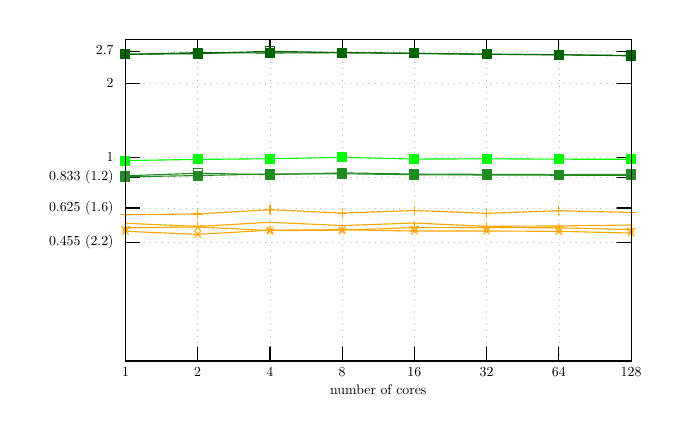
\begin{tikzpicture}[gnuplot]
%% generated with GNUPLOT 6.0p1 (Lua 5.4; terminal rev. Jun 2020, script rev. 118)
%% ven. 10 janv. 2025 17:58:53
\tikzset{every node/.append style={scale=0.50}}
\path (0.000,0.000) rectangle (8.125,4.725);
\gpcolor{color=gp lt color axes}
\gpsetlinetype{gp lt axes}
\gpsetdashtype{gp dt axes}
\gpsetlinewidth{0.50}
\draw[gp path] (1.242,2.001)--(7.664,2.001);
\gpcolor{color=gp lt color border}
\gpsetlinetype{gp lt border}
\gpsetdashtype{gp dt solid}
\gpsetlinewidth{1.00}
\draw[gp path] (1.242,2.001)--(1.422,2.001);
\draw[gp path] (7.664,2.001)--(7.484,2.001);
\node[gp node right] at (1.150,2.001) {0.455 (2.2)};
\gpcolor{color=gp lt color axes}
\gpsetlinetype{gp lt axes}
\gpsetdashtype{gp dt axes}
\gpsetlinewidth{0.50}
\draw[gp path] (1.242,2.435)--(7.664,2.435);
\gpcolor{color=gp lt color border}
\gpsetlinetype{gp lt border}
\gpsetdashtype{gp dt solid}
\gpsetlinewidth{1.00}
\draw[gp path] (1.242,2.435)--(1.422,2.435);
\draw[gp path] (7.664,2.435)--(7.484,2.435);
\node[gp node right] at (1.150,2.435) {0.625 (1.6)};
\gpcolor{color=gp lt color axes}
\gpsetlinetype{gp lt axes}
\gpsetdashtype{gp dt axes}
\gpsetlinewidth{0.50}
\draw[gp path] (1.242,2.826)--(7.664,2.826);
\gpcolor{color=gp lt color border}
\gpsetlinetype{gp lt border}
\gpsetdashtype{gp dt solid}
\gpsetlinewidth{1.00}
\draw[gp path] (1.242,2.826)--(1.422,2.826);
\draw[gp path] (7.664,2.826)--(7.484,2.826);
\node[gp node right] at (1.150,2.826) {0.833 (1.2)};
\gpcolor{color=gp lt color axes}
\gpsetlinetype{gp lt axes}
\gpsetdashtype{gp dt axes}
\gpsetlinewidth{0.50}
\draw[gp path] (1.242,3.074)--(7.664,3.074);
\gpcolor{color=gp lt color border}
\gpsetlinetype{gp lt border}
\gpsetdashtype{gp dt solid}
\gpsetlinewidth{1.00}
\draw[gp path] (1.242,3.074)--(1.422,3.074);
\draw[gp path] (7.664,3.074)--(7.484,3.074);
\node[gp node right] at (1.150,3.074) {$1$};
\gpcolor{color=gp lt color axes}
\gpsetlinetype{gp lt axes}
\gpsetdashtype{gp dt axes}
\gpsetlinewidth{0.50}
\draw[gp path] (1.242,4.018)--(7.664,4.018);
\gpcolor{color=gp lt color border}
\gpsetlinetype{gp lt border}
\gpsetdashtype{gp dt solid}
\gpsetlinewidth{1.00}
\draw[gp path] (1.242,4.018)--(1.422,4.018);
\draw[gp path] (7.664,4.018)--(7.484,4.018);
\node[gp node right] at (1.150,4.018) {$2$};
\gpcolor{color=gp lt color axes}
\gpsetlinetype{gp lt axes}
\gpsetdashtype{gp dt axes}
\gpsetlinewidth{0.50}
\draw[gp path] (1.242,4.427)--(7.664,4.427);
\gpcolor{color=gp lt color border}
\gpsetlinetype{gp lt border}
\gpsetdashtype{gp dt solid}
\gpsetlinewidth{1.00}
\draw[gp path] (1.242,4.427)--(1.422,4.427);
\draw[gp path] (7.664,4.427)--(7.484,4.427);
\node[gp node right] at (1.150,4.427) {$2.7$};
\gpcolor{color=gp lt color axes}
\gpsetlinetype{gp lt axes}
\gpsetdashtype{gp dt axes}
\gpsetlinewidth{0.50}
\draw[gp path] (1.242,0.492)--(1.242,4.570);
\gpcolor{color=gp lt color border}
\gpsetlinetype{gp lt border}
\gpsetdashtype{gp dt solid}
\gpsetlinewidth{1.00}
\draw[gp path] (1.242,0.492)--(1.242,0.672);
\draw[gp path] (1.242,4.570)--(1.242,4.390);
\node[gp node center] at (1.242,0.338) {1};
\gpcolor{color=gp lt color axes}
\gpsetlinetype{gp lt axes}
\gpsetdashtype{gp dt axes}
\gpsetlinewidth{0.50}
\draw[gp path] (2.159,0.492)--(2.159,4.570);
\gpcolor{color=gp lt color border}
\gpsetlinetype{gp lt border}
\gpsetdashtype{gp dt solid}
\gpsetlinewidth{1.00}
\draw[gp path] (2.159,0.492)--(2.159,0.672);
\draw[gp path] (2.159,4.570)--(2.159,4.390);
\node[gp node center] at (2.159,0.338) {2};
\gpcolor{color=gp lt color axes}
\gpsetlinetype{gp lt axes}
\gpsetdashtype{gp dt axes}
\gpsetlinewidth{0.50}
\draw[gp path] (3.077,0.492)--(3.077,4.570);
\gpcolor{color=gp lt color border}
\gpsetlinetype{gp lt border}
\gpsetdashtype{gp dt solid}
\gpsetlinewidth{1.00}
\draw[gp path] (3.077,0.492)--(3.077,0.672);
\draw[gp path] (3.077,4.570)--(3.077,4.390);
\node[gp node center] at (3.077,0.338) {4};
\gpcolor{color=gp lt color axes}
\gpsetlinetype{gp lt axes}
\gpsetdashtype{gp dt axes}
\gpsetlinewidth{0.50}
\draw[gp path] (3.994,0.492)--(3.994,4.570);
\gpcolor{color=gp lt color border}
\gpsetlinetype{gp lt border}
\gpsetdashtype{gp dt solid}
\gpsetlinewidth{1.00}
\draw[gp path] (3.994,0.492)--(3.994,0.672);
\draw[gp path] (3.994,4.570)--(3.994,4.390);
\node[gp node center] at (3.994,0.338) {8};
\gpcolor{color=gp lt color axes}
\gpsetlinetype{gp lt axes}
\gpsetdashtype{gp dt axes}
\gpsetlinewidth{0.50}
\draw[gp path] (4.911,0.492)--(4.911,4.570);
\gpcolor{color=gp lt color border}
\gpsetlinetype{gp lt border}
\gpsetdashtype{gp dt solid}
\gpsetlinewidth{1.00}
\draw[gp path] (4.911,0.492)--(4.911,0.672);
\draw[gp path] (4.911,4.570)--(4.911,4.390);
\node[gp node center] at (4.911,0.338) {16};
\gpcolor{color=gp lt color axes}
\gpsetlinetype{gp lt axes}
\gpsetdashtype{gp dt axes}
\gpsetlinewidth{0.50}
\draw[gp path] (5.828,0.492)--(5.828,4.570);
\gpcolor{color=gp lt color border}
\gpsetlinetype{gp lt border}
\gpsetdashtype{gp dt solid}
\gpsetlinewidth{1.00}
\draw[gp path] (5.828,0.492)--(5.828,0.672);
\draw[gp path] (5.828,4.570)--(5.828,4.390);
\node[gp node center] at (5.828,0.338) {32};
\gpcolor{color=gp lt color axes}
\gpsetlinetype{gp lt axes}
\gpsetdashtype{gp dt axes}
\gpsetlinewidth{0.50}
\draw[gp path] (6.746,0.492)--(6.746,4.570);
\gpcolor{color=gp lt color border}
\gpsetlinetype{gp lt border}
\gpsetdashtype{gp dt solid}
\gpsetlinewidth{1.00}
\draw[gp path] (6.746,0.492)--(6.746,0.672);
\draw[gp path] (6.746,4.570)--(6.746,4.390);
\node[gp node center] at (6.746,0.338) {64};
\gpcolor{color=gp lt color axes}
\gpsetlinetype{gp lt axes}
\gpsetdashtype{gp dt axes}
\gpsetlinewidth{0.50}
\draw[gp path] (7.663,0.492)--(7.663,4.570);
\gpcolor{color=gp lt color border}
\gpsetlinetype{gp lt border}
\gpsetdashtype{gp dt solid}
\gpsetlinewidth{1.00}
\draw[gp path] (7.663,0.492)--(7.663,0.672);
\draw[gp path] (7.663,4.570)--(7.663,4.390);
\node[gp node center] at (7.663,0.338) {128};
\draw[gp path] (1.242,4.570)--(1.242,0.492)--(7.664,0.492)--(7.664,4.570)--cycle;
\gpcolor{rgb color={1.000,0.647,0.000}}
\draw[gp path] (1.242,2.349)--(2.159,2.359)--(3.077,2.414)--(3.994,2.370)--(4.911,2.403)%
  --(5.828,2.367)--(6.746,2.400)--(7.663,2.378);
\gpsetpointsize{4.00}
\gp3point{gp mark 1}{}{(1.242,2.349)}
\gp3point{gp mark 1}{}{(2.159,2.359)}
\gp3point{gp mark 1}{}{(3.077,2.414)}
\gp3point{gp mark 1}{}{(3.994,2.370)}
\gp3point{gp mark 1}{}{(4.911,2.403)}
\gp3point{gp mark 1}{}{(5.828,2.367)}
\gp3point{gp mark 1}{}{(6.746,2.400)}
\gp3point{gp mark 1}{}{(7.663,2.378)}
\draw[gp path] (1.242,2.139)--(2.159,2.100)--(3.077,2.153)--(3.994,2.159)--(4.911,2.142)%
  --(5.828,2.143)--(6.746,2.138)--(7.663,2.117);
\gp3point{gp mark 2}{}{(1.242,2.139)}
\gp3point{gp mark 2}{}{(2.159,2.100)}
\gp3point{gp mark 2}{}{(3.077,2.153)}
\gp3point{gp mark 2}{}{(3.994,2.159)}
\gp3point{gp mark 2}{}{(4.911,2.142)}
\gp3point{gp mark 2}{}{(5.828,2.143)}
\gp3point{gp mark 2}{}{(6.746,2.138)}
\gp3point{gp mark 2}{}{(7.663,2.117)}
\draw[gp path] (1.242,2.183)--(2.159,2.194)--(3.077,2.147)--(3.994,2.154)--(4.911,2.186)%
  --(5.828,2.187)--(6.746,2.183)--(7.663,2.161);
\gp3point{gp mark 3}{}{(1.242,2.183)}
\gp3point{gp mark 3}{}{(2.159,2.194)}
\gp3point{gp mark 3}{}{(3.077,2.147)}
\gp3point{gp mark 3}{}{(3.994,2.154)}
\gp3point{gp mark 3}{}{(4.911,2.186)}
\gp3point{gp mark 3}{}{(5.828,2.187)}
\gp3point{gp mark 3}{}{(6.746,2.183)}
\gp3point{gp mark 3}{}{(7.663,2.161)}
\draw[gp path] (1.242,2.241)--(2.159,2.201)--(3.077,2.253)--(3.994,2.212)--(4.911,2.244)%
  --(5.828,2.202)--(6.746,2.207)--(7.663,2.219);
\gp3point{gp mark 0}{}{(1.242,2.241)}
\gp3point{gp mark 0}{}{(2.159,2.201)}
\gp3point{gp mark 0}{}{(3.077,2.253)}
\gp3point{gp mark 0}{}{(3.994,2.212)}
\gp3point{gp mark 0}{}{(4.911,2.244)}
\gp3point{gp mark 0}{}{(5.828,2.202)}
\gp3point{gp mark 0}{}{(6.746,2.207)}
\gp3point{gp mark 0}{}{(7.663,2.219)}
\gpcolor{rgb color={0.000,1.000,0.000}}
\draw[gp path] (1.242,3.037)--(2.159,3.052)--(3.077,3.060)--(3.994,3.078)--(4.911,3.056)%
  --(5.828,3.059)--(6.746,3.055)--(7.663,3.053);
\gp3point{gp mark 5}{}{(1.242,3.037)}
\gp3point{gp mark 5}{}{(2.159,3.052)}
\gp3point{gp mark 5}{}{(3.077,3.060)}
\gp3point{gp mark 5}{}{(3.994,3.078)}
\gp3point{gp mark 5}{}{(4.911,3.056)}
\gp3point{gp mark 5}{}{(5.828,3.059)}
\gp3point{gp mark 5}{}{(6.746,3.055)}
\gp3point{gp mark 5}{}{(7.663,3.053)}
\gpcolor{rgb color={0.000,0.392,0.000}}
\draw[gp path] (1.242,4.387)--(2.159,4.395)--(3.077,4.425)--(3.994,4.408)--(4.911,4.399)%
  --(5.828,4.388)--(6.746,4.382)--(7.663,4.367);
\gp3point{gp mark 4}{}{(1.242,4.387)}
\gp3point{gp mark 4}{}{(2.159,4.395)}
\gp3point{gp mark 4}{}{(3.077,4.425)}
\gp3point{gp mark 4}{}{(3.994,4.408)}
\gp3point{gp mark 4}{}{(4.911,4.399)}
\gp3point{gp mark 4}{}{(5.828,4.388)}
\gp3point{gp mark 4}{}{(6.746,4.382)}
\gp3point{gp mark 4}{}{(7.663,4.367)}
\draw[gp path] (1.242,4.386)--(2.159,4.408)--(3.077,4.403)--(3.994,4.408)--(4.911,4.398)%
  --(5.828,4.387)--(6.746,4.380)--(7.663,4.372);
\gp3point{gp mark 5}{}{(1.242,4.386)}
\gp3point{gp mark 5}{}{(2.159,4.408)}
\gp3point{gp mark 5}{}{(3.077,4.403)}
\gp3point{gp mark 5}{}{(3.994,4.408)}
\gp3point{gp mark 5}{}{(4.911,4.398)}
\gp3point{gp mark 5}{}{(5.828,4.387)}
\gp3point{gp mark 5}{}{(6.746,4.380)}
\gp3point{gp mark 5}{}{(7.663,4.372)}
\gpcolor{rgb color={0.133,0.545,0.133}}
\draw[gp path] (1.242,2.844)--(2.159,2.876)--(3.077,2.858)--(3.994,2.881)--(4.911,2.866)%
  --(5.828,2.862)--(6.746,2.859)--(7.663,2.862);
\gp3point{gp mark 4}{}{(1.242,2.844)}
\gp3point{gp mark 4}{}{(2.159,2.876)}
\gp3point{gp mark 4}{}{(3.077,2.858)}
\gp3point{gp mark 4}{}{(3.994,2.881)}
\gp3point{gp mark 4}{}{(4.911,2.866)}
\gp3point{gp mark 4}{}{(5.828,2.862)}
\gp3point{gp mark 4}{}{(6.746,2.859)}
\gp3point{gp mark 4}{}{(7.663,2.862)}
\draw[gp path] (1.242,2.830)--(2.159,2.847)--(3.077,2.867)--(3.994,2.870)--(4.911,2.857)%
  --(5.828,2.854)--(6.746,2.851)--(7.663,2.850);
\gp3point{gp mark 5}{}{(1.242,2.830)}
\gp3point{gp mark 5}{}{(2.159,2.847)}
\gp3point{gp mark 5}{}{(3.077,2.867)}
\gp3point{gp mark 5}{}{(3.994,2.870)}
\gp3point{gp mark 5}{}{(4.911,2.857)}
\gp3point{gp mark 5}{}{(5.828,2.854)}
\gp3point{gp mark 5}{}{(6.746,2.851)}
\gp3point{gp mark 5}{}{(7.663,2.850)}
\gpcolor{color=gp lt color border}
\draw[gp path] (1.242,4.570)--(1.242,0.492)--(7.664,0.492)--(7.664,4.570)--cycle;
\node[gp node center] at (4.453,0.107) {number of cores};
%% coordinates of the plot area
\gpdefrectangularnode{gp plot 1}{\pgfpoint{1.242cm}{0.492cm}}{\pgfpoint{7.664cm}{4.570cm}}
\end{tikzpicture}
%% gnuplot variables
}\\
	\subfloat[Elementary matrix creation(in s)]{
		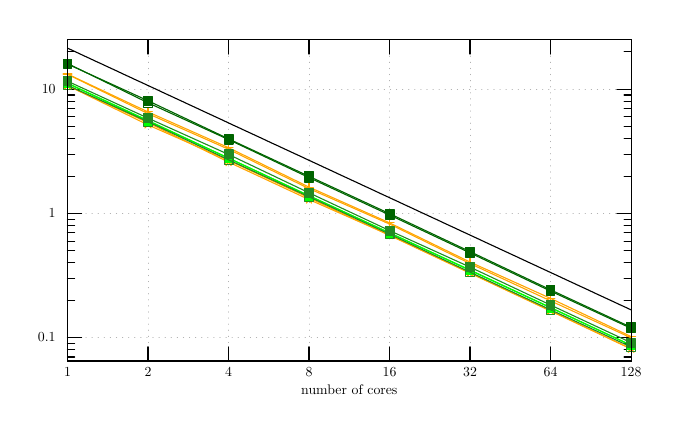
\begin{tikzpicture}[gnuplot]
%% generated with GNUPLOT 6.0p1 (Lua 5.4; terminal rev. Jun 2020, script rev. 118)
%% ven. 10 janv. 2025 17:58:53
\tikzset{every node/.append style={scale=0.50}}
\path (0.000,0.000) rectangle (8.125,4.725);
\gpcolor{color=gp lt color border}
\gpsetlinetype{gp lt border}
\gpsetdashtype{gp dt solid}
\gpsetlinewidth{1.00}
\draw[gp path] (0.506,0.543)--(0.596,0.543);
\draw[gp path] (7.664,0.543)--(7.574,0.543);
\draw[gp path] (0.506,0.634)--(0.596,0.634);
\draw[gp path] (7.664,0.634)--(7.574,0.634);
\draw[gp path] (0.506,0.715)--(0.596,0.715);
\draw[gp path] (7.664,0.715)--(7.574,0.715);
\gpcolor{color=gp lt color axes}
\gpsetlinetype{gp lt axes}
\gpsetdashtype{gp dt axes}
\gpsetlinewidth{0.50}
\draw[gp path] (0.506,0.787)--(7.664,0.787);
\gpcolor{color=gp lt color border}
\gpsetlinetype{gp lt border}
\gpsetdashtype{gp dt solid}
\gpsetlinewidth{1.00}
\draw[gp path] (0.506,0.787)--(0.686,0.787);
\draw[gp path] (7.664,0.787)--(7.484,0.787);
\node[gp node right] at (0.414,0.787) {$0.1$};
\draw[gp path] (0.506,1.262)--(0.596,1.262);
\draw[gp path] (7.664,1.262)--(7.574,1.262);
\draw[gp path] (0.506,1.540)--(0.596,1.540);
\draw[gp path] (7.664,1.540)--(7.574,1.540);
\draw[gp path] (0.506,1.737)--(0.596,1.737);
\draw[gp path] (7.664,1.737)--(7.574,1.737);
\draw[gp path] (0.506,1.890)--(0.596,1.890);
\draw[gp path] (7.664,1.890)--(7.574,1.890);
\draw[gp path] (0.506,2.015)--(0.596,2.015);
\draw[gp path] (7.664,2.015)--(7.574,2.015);
\draw[gp path] (0.506,2.120)--(0.596,2.120);
\draw[gp path] (7.664,2.120)--(7.574,2.120);
\draw[gp path] (0.506,2.212)--(0.596,2.212);
\draw[gp path] (7.664,2.212)--(7.574,2.212);
\draw[gp path] (0.506,2.292)--(0.596,2.292);
\draw[gp path] (7.664,2.292)--(7.574,2.292);
\gpcolor{color=gp lt color axes}
\gpsetlinetype{gp lt axes}
\gpsetdashtype{gp dt axes}
\gpsetlinewidth{0.50}
\draw[gp path] (0.506,2.365)--(7.664,2.365);
\gpcolor{color=gp lt color border}
\gpsetlinetype{gp lt border}
\gpsetdashtype{gp dt solid}
\gpsetlinewidth{1.00}
\draw[gp path] (0.506,2.365)--(0.686,2.365);
\draw[gp path] (7.664,2.365)--(7.484,2.365);
\node[gp node right] at (0.414,2.365) {$1$};
\draw[gp path] (0.506,2.840)--(0.596,2.840);
\draw[gp path] (7.664,2.840)--(7.574,2.840);
\draw[gp path] (0.506,3.117)--(0.596,3.117);
\draw[gp path] (7.664,3.117)--(7.574,3.117);
\draw[gp path] (0.506,3.314)--(0.596,3.314);
\draw[gp path] (7.664,3.314)--(7.574,3.314);
\draw[gp path] (0.506,3.467)--(0.596,3.467);
\draw[gp path] (7.664,3.467)--(7.574,3.467);
\draw[gp path] (0.506,3.592)--(0.596,3.592);
\draw[gp path] (7.664,3.592)--(7.574,3.592);
\draw[gp path] (0.506,3.698)--(0.596,3.698);
\draw[gp path] (7.664,3.698)--(7.574,3.698);
\draw[gp path] (0.506,3.789)--(0.596,3.789);
\draw[gp path] (7.664,3.789)--(7.574,3.789);
\draw[gp path] (0.506,3.870)--(0.596,3.870);
\draw[gp path] (7.664,3.870)--(7.574,3.870);
\gpcolor{color=gp lt color axes}
\gpsetlinetype{gp lt axes}
\gpsetdashtype{gp dt axes}
\gpsetlinewidth{0.50}
\draw[gp path] (0.506,3.942)--(7.664,3.942);
\gpcolor{color=gp lt color border}
\gpsetlinetype{gp lt border}
\gpsetdashtype{gp dt solid}
\gpsetlinewidth{1.00}
\draw[gp path] (0.506,3.942)--(0.686,3.942);
\draw[gp path] (7.664,3.942)--(7.484,3.942);
\node[gp node right] at (0.414,3.942) {$10$};
\draw[gp path] (0.506,4.417)--(0.596,4.417);
\draw[gp path] (7.664,4.417)--(7.574,4.417);
\gpcolor{color=gp lt color axes}
\gpsetlinetype{gp lt axes}
\gpsetdashtype{gp dt axes}
\gpsetlinewidth{0.50}
\draw[gp path] (0.506,0.492)--(0.506,4.570);
\gpcolor{color=gp lt color border}
\gpsetlinetype{gp lt border}
\gpsetdashtype{gp dt solid}
\gpsetlinewidth{1.00}
\draw[gp path] (0.506,0.492)--(0.506,0.672);
\draw[gp path] (0.506,4.570)--(0.506,4.390);
\node[gp node center] at (0.506,0.338) {1};
\gpcolor{color=gp lt color axes}
\gpsetlinetype{gp lt axes}
\gpsetdashtype{gp dt axes}
\gpsetlinewidth{0.50}
\draw[gp path] (1.528,0.492)--(1.528,4.570);
\gpcolor{color=gp lt color border}
\gpsetlinetype{gp lt border}
\gpsetdashtype{gp dt solid}
\gpsetlinewidth{1.00}
\draw[gp path] (1.528,0.492)--(1.528,0.672);
\draw[gp path] (1.528,4.570)--(1.528,4.390);
\node[gp node center] at (1.528,0.338) {2};
\gpcolor{color=gp lt color axes}
\gpsetlinetype{gp lt axes}
\gpsetdashtype{gp dt axes}
\gpsetlinewidth{0.50}
\draw[gp path] (2.551,0.492)--(2.551,4.570);
\gpcolor{color=gp lt color border}
\gpsetlinetype{gp lt border}
\gpsetdashtype{gp dt solid}
\gpsetlinewidth{1.00}
\draw[gp path] (2.551,0.492)--(2.551,0.672);
\draw[gp path] (2.551,4.570)--(2.551,4.390);
\node[gp node center] at (2.551,0.338) {4};
\gpcolor{color=gp lt color axes}
\gpsetlinetype{gp lt axes}
\gpsetdashtype{gp dt axes}
\gpsetlinewidth{0.50}
\draw[gp path] (3.573,0.492)--(3.573,4.570);
\gpcolor{color=gp lt color border}
\gpsetlinetype{gp lt border}
\gpsetdashtype{gp dt solid}
\gpsetlinewidth{1.00}
\draw[gp path] (3.573,0.492)--(3.573,0.672);
\draw[gp path] (3.573,4.570)--(3.573,4.390);
\node[gp node center] at (3.573,0.338) {8};
\gpcolor{color=gp lt color axes}
\gpsetlinetype{gp lt axes}
\gpsetdashtype{gp dt axes}
\gpsetlinewidth{0.50}
\draw[gp path] (4.596,0.492)--(4.596,4.570);
\gpcolor{color=gp lt color border}
\gpsetlinetype{gp lt border}
\gpsetdashtype{gp dt solid}
\gpsetlinewidth{1.00}
\draw[gp path] (4.596,0.492)--(4.596,0.672);
\draw[gp path] (4.596,4.570)--(4.596,4.390);
\node[gp node center] at (4.596,0.338) {16};
\gpcolor{color=gp lt color axes}
\gpsetlinetype{gp lt axes}
\gpsetdashtype{gp dt axes}
\gpsetlinewidth{0.50}
\draw[gp path] (5.618,0.492)--(5.618,4.570);
\gpcolor{color=gp lt color border}
\gpsetlinetype{gp lt border}
\gpsetdashtype{gp dt solid}
\gpsetlinewidth{1.00}
\draw[gp path] (5.618,0.492)--(5.618,0.672);
\draw[gp path] (5.618,4.570)--(5.618,4.390);
\node[gp node center] at (5.618,0.338) {32};
\gpcolor{color=gp lt color axes}
\gpsetlinetype{gp lt axes}
\gpsetdashtype{gp dt axes}
\gpsetlinewidth{0.50}
\draw[gp path] (6.640,0.492)--(6.640,4.570);
\gpcolor{color=gp lt color border}
\gpsetlinetype{gp lt border}
\gpsetdashtype{gp dt solid}
\gpsetlinewidth{1.00}
\draw[gp path] (6.640,0.492)--(6.640,0.672);
\draw[gp path] (6.640,4.570)--(6.640,4.390);
\node[gp node center] at (6.640,0.338) {64};
\gpcolor{color=gp lt color axes}
\gpsetlinetype{gp lt axes}
\gpsetdashtype{gp dt axes}
\gpsetlinewidth{0.50}
\draw[gp path] (7.663,0.492)--(7.663,4.570);
\gpcolor{color=gp lt color border}
\gpsetlinetype{gp lt border}
\gpsetdashtype{gp dt solid}
\gpsetlinewidth{1.00}
\draw[gp path] (7.663,0.492)--(7.663,0.672);
\draw[gp path] (7.663,4.570)--(7.663,4.390);
\node[gp node center] at (7.663,0.338) {128};
\draw[gp path] (0.506,4.570)--(0.506,0.492)--(7.664,0.492)--(7.664,4.570)--cycle;
\gpcolor{rgb color={1.000,0.647,0.000}}
\draw[gp path] (0.506,4.136)--(1.528,3.655)--(2.551,3.201)--(3.573,2.700)--(4.596,2.246)%
  --(5.618,1.748)--(6.640,1.287)--(7.663,0.802);
\gpsetpointsize{4.00}
\gp3point{gp mark 1}{}{(0.506,4.136)}
\gp3point{gp mark 1}{}{(1.528,3.655)}
\gp3point{gp mark 1}{}{(2.551,3.201)}
\gp3point{gp mark 1}{}{(3.573,2.700)}
\gp3point{gp mark 1}{}{(4.596,2.246)}
\gp3point{gp mark 1}{}{(5.618,1.748)}
\gp3point{gp mark 1}{}{(6.640,1.287)}
\gp3point{gp mark 1}{}{(7.663,0.802)}
\draw[gp path] (0.506,3.990)--(1.528,3.490)--(2.551,3.040)--(3.573,2.564)--(4.596,2.087)%
  --(5.618,1.607)--(6.640,1.127)--(7.663,0.645);
\gp3point{gp mark 2}{}{(0.506,3.990)}
\gp3point{gp mark 2}{}{(1.528,3.490)}
\gp3point{gp mark 2}{}{(2.551,3.040)}
\gp3point{gp mark 2}{}{(3.573,2.564)}
\gp3point{gp mark 2}{}{(4.596,2.087)}
\gp3point{gp mark 2}{}{(5.618,1.607)}
\gp3point{gp mark 2}{}{(6.640,1.127)}
\gp3point{gp mark 2}{}{(7.663,0.645)}
\draw[gp path] (0.506,3.991)--(1.528,3.518)--(2.551,3.018)--(3.573,2.542)--(4.596,2.091)%
  --(5.618,1.611)--(6.640,1.131)--(7.663,0.648);
\gp3point{gp mark 3}{}{(0.506,3.991)}
\gp3point{gp mark 3}{}{(1.528,3.518)}
\gp3point{gp mark 3}{}{(2.551,3.018)}
\gp3point{gp mark 3}{}{(3.573,2.542)}
\gp3point{gp mark 3}{}{(4.596,2.091)}
\gp3point{gp mark 3}{}{(5.618,1.611)}
\gp3point{gp mark 3}{}{(6.640,1.131)}
\gp3point{gp mark 3}{}{(7.663,0.648)}
\draw[gp path] (0.506,4.133)--(1.528,3.633)--(2.551,3.181)--(3.573,2.681)--(4.596,2.231)%
  --(5.618,1.729)--(6.640,1.256)--(7.663,0.786);
\gp3point{gp mark 0}{}{(0.506,4.133)}
\gp3point{gp mark 0}{}{(1.528,3.633)}
\gp3point{gp mark 0}{}{(2.551,3.181)}
\gp3point{gp mark 0}{}{(3.573,2.681)}
\gp3point{gp mark 0}{}{(4.596,2.231)}
\gp3point{gp mark 0}{}{(5.618,1.729)}
\gp3point{gp mark 0}{}{(6.640,1.256)}
\gp3point{gp mark 0}{}{(7.663,0.786)}
\gpcolor{rgb color={0.000,1.000,0.000}}
\draw[gp path] (0.506,4.017)--(1.528,3.537)--(2.551,3.069)--(3.573,2.591)--(4.596,2.118)%
  --(5.618,1.642)--(6.640,1.168)--(7.663,0.691);
\gp3point{gp mark 4}{}{(0.506,4.017)}
\gp3point{gp mark 4}{}{(1.528,3.537)}
\gp3point{gp mark 4}{}{(2.551,3.069)}
\gp3point{gp mark 4}{}{(3.573,2.591)}
\gp3point{gp mark 4}{}{(4.596,2.118)}
\gp3point{gp mark 4}{}{(5.618,1.642)}
\gp3point{gp mark 4}{}{(6.640,1.168)}
\gp3point{gp mark 4}{}{(7.663,0.691)}
\draw[gp path] (0.506,4.020)--(1.528,3.547)--(2.551,3.068)--(3.573,2.590)--(4.596,2.120)%
  --(5.618,1.648)--(6.640,1.172)--(7.663,0.692);
\gp3point{gp mark 5}{}{(0.506,4.020)}
\gp3point{gp mark 5}{}{(1.528,3.547)}
\gp3point{gp mark 5}{}{(2.551,3.068)}
\gp3point{gp mark 5}{}{(3.573,2.590)}
\gp3point{gp mark 5}{}{(4.596,2.120)}
\gp3point{gp mark 5}{}{(5.618,1.648)}
\gp3point{gp mark 5}{}{(6.640,1.172)}
\gp3point{gp mark 5}{}{(7.663,0.692)}
\gpcolor{rgb color={0.000,0.392,0.000}}
\draw[gp path] (0.506,4.270)--(1.528,3.771)--(2.551,3.304)--(3.573,2.821)--(4.596,2.346)%
  --(5.618,1.865)--(6.640,1.380)--(7.663,0.907);
\gp3point{gp mark 4}{}{(0.506,4.270)}
\gp3point{gp mark 4}{}{(1.528,3.771)}
\gp3point{gp mark 4}{}{(2.551,3.304)}
\gp3point{gp mark 4}{}{(3.573,2.821)}
\gp3point{gp mark 4}{}{(4.596,2.346)}
\gp3point{gp mark 4}{}{(5.618,1.865)}
\gp3point{gp mark 4}{}{(6.640,1.380)}
\gp3point{gp mark 4}{}{(7.663,0.907)}
\draw[gp path] (0.506,4.263)--(1.528,3.797)--(2.551,3.313)--(3.573,2.837)--(4.596,2.363)%
  --(5.618,1.881)--(6.640,1.396)--(7.663,0.920);
\gp3point{gp mark 5}{}{(0.506,4.263)}
\gp3point{gp mark 5}{}{(1.528,3.797)}
\gp3point{gp mark 5}{}{(2.551,3.313)}
\gp3point{gp mark 5}{}{(3.573,2.837)}
\gp3point{gp mark 5}{}{(4.596,2.363)}
\gp3point{gp mark 5}{}{(5.618,1.881)}
\gp3point{gp mark 5}{}{(6.640,1.396)}
\gp3point{gp mark 5}{}{(7.663,0.920)}
\gpcolor{rgb color={0.000,0.000,0.000}}
\draw[gp path] (0.506,4.465)--(0.578,4.432)--(0.651,4.398)--(0.723,4.364)--(0.795,4.331)%
  --(0.867,4.297)--(0.940,4.264)--(1.012,4.230)--(1.084,4.197)--(1.157,4.163)--(1.229,4.129)%
  --(1.301,4.096)--(1.373,4.062)--(1.446,4.029)--(1.518,3.995)--(1.590,3.962)--(1.663,3.928)%
  --(1.735,3.894)--(1.807,3.861)--(1.880,3.827)--(1.952,3.794)--(2.024,3.760)--(2.096,3.727)%
  --(2.169,3.693)--(2.241,3.659)--(2.313,3.626)--(2.386,3.592)--(2.458,3.559)--(2.530,3.525)%
  --(2.602,3.491)--(2.675,3.458)--(2.747,3.424)--(2.819,3.391)--(2.892,3.357)--(2.964,3.324)%
  --(3.036,3.290)--(3.108,3.256)--(3.181,3.223)--(3.253,3.189)--(3.325,3.156)--(3.398,3.122)%
  --(3.470,3.089)--(3.542,3.055)--(3.615,3.021)--(3.687,2.988)--(3.759,2.954)--(3.831,2.921)%
  --(3.904,2.887)--(3.976,2.853)--(4.048,2.820)--(4.121,2.786)--(4.193,2.753)--(4.265,2.719)%
  --(4.337,2.686)--(4.410,2.652)--(4.482,2.618)--(4.554,2.585)--(4.627,2.551)--(4.699,2.518)%
  --(4.771,2.484)--(4.843,2.451)--(4.916,2.417)--(4.988,2.383)--(5.060,2.350)--(5.133,2.316)%
  --(5.205,2.283)--(5.277,2.249)--(5.350,2.215)--(5.422,2.182)--(5.494,2.148)--(5.566,2.115)%
  --(5.639,2.081)--(5.711,2.048)--(5.783,2.014)--(5.856,1.980)--(5.928,1.947)--(6.000,1.913)%
  --(6.072,1.880)--(6.145,1.846)--(6.217,1.813)--(6.289,1.779)--(6.362,1.745)--(6.434,1.712)%
  --(6.506,1.678)--(6.578,1.645)--(6.651,1.611)--(6.723,1.578)--(6.795,1.544)--(6.868,1.510)%
  --(6.940,1.477)--(7.012,1.443)--(7.085,1.410)--(7.157,1.376)--(7.229,1.342)--(7.301,1.309)%
  --(7.374,1.275)--(7.446,1.242)--(7.518,1.208)--(7.591,1.175)--(7.663,1.141);
\gpcolor{rgb color={0.133,0.545,0.133}}
\draw[gp path] (0.506,3.993)--(1.528,3.530)--(2.551,3.047)--(3.573,2.577)--(4.596,2.103)%
  --(5.618,1.620)--(6.640,1.143)--(7.663,0.670);
\gp3point{gp mark 4}{}{(0.506,3.993)}
\gp3point{gp mark 4}{}{(1.528,3.530)}
\gp3point{gp mark 4}{}{(2.551,3.047)}
\gp3point{gp mark 4}{}{(3.573,2.577)}
\gp3point{gp mark 4}{}{(4.596,2.103)}
\gp3point{gp mark 4}{}{(5.618,1.620)}
\gp3point{gp mark 4}{}{(6.640,1.143)}
\gp3point{gp mark 4}{}{(7.663,0.670)}
\draw[gp path] (0.506,4.045)--(1.528,3.576)--(2.551,3.115)--(3.573,2.628)--(4.596,2.148)%
  --(5.618,1.684)--(6.640,1.203)--(7.663,0.725);
\gp3point{gp mark 5}{}{(0.506,4.045)}
\gp3point{gp mark 5}{}{(1.528,3.576)}
\gp3point{gp mark 5}{}{(2.551,3.115)}
\gp3point{gp mark 5}{}{(3.573,2.628)}
\gp3point{gp mark 5}{}{(4.596,2.148)}
\gp3point{gp mark 5}{}{(5.618,1.684)}
\gp3point{gp mark 5}{}{(6.640,1.203)}
\gp3point{gp mark 5}{}{(7.663,0.725)}
\gpcolor{color=gp lt color border}
\draw[gp path] (0.506,4.570)--(0.506,0.492)--(7.664,0.492)--(7.664,4.570)--cycle;
\node[gp node center] at (4.085,0.107) {number of cores};
%% coordinates of the plot area
\gpdefrectangularnode{gp plot 1}{\pgfpoint{0.506cm}{0.492cm}}{\pgfpoint{7.664cm}{4.570cm}}
\end{tikzpicture}
%% gnuplot variables

	}
	\subfloat[Elementary matrix creation(Ratio vs MFEM)\label{elapsd2rm}]{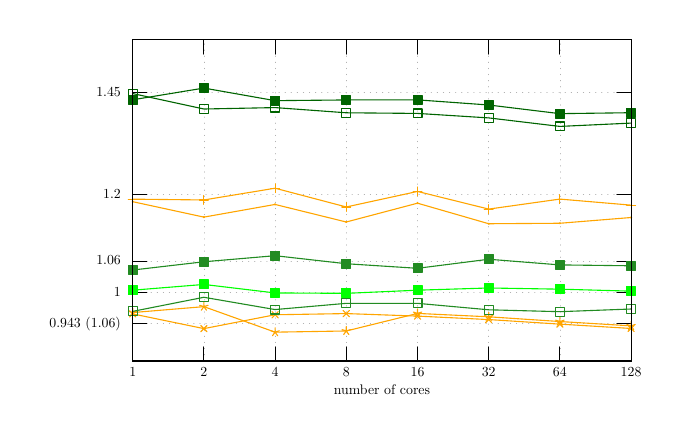
\begin{tikzpicture}[gnuplot]
%% generated with GNUPLOT 6.0p1 (Lua 5.4; terminal rev. Jun 2020, script rev. 118)
%% ven. 10 janv. 2025 17:58:53
\tikzset{every node/.append style={scale=0.50}}
\path (0.000,0.000) rectangle (8.125,4.725);
\gpcolor{color=gp lt color axes}
\gpsetlinetype{gp lt axes}
\gpsetdashtype{gp dt axes}
\gpsetlinewidth{0.50}
\draw[gp path] (1.334,0.966)--(7.664,0.966);
\gpcolor{color=gp lt color border}
\gpsetlinetype{gp lt border}
\gpsetdashtype{gp dt solid}
\gpsetlinewidth{1.00}
\draw[gp path] (1.334,0.966)--(1.514,0.966);
\draw[gp path] (7.664,0.966)--(7.484,0.966);
\node[gp node right] at (1.242,0.966) {0.943 (1.06)};
\gpcolor{color=gp lt color axes}
\gpsetlinetype{gp lt axes}
\gpsetdashtype{gp dt axes}
\gpsetlinewidth{0.50}
\draw[gp path] (1.334,1.364)--(7.664,1.364);
\gpcolor{color=gp lt color border}
\gpsetlinetype{gp lt border}
\gpsetdashtype{gp dt solid}
\gpsetlinewidth{1.00}
\draw[gp path] (1.334,1.364)--(1.514,1.364);
\draw[gp path] (7.664,1.364)--(7.484,1.364);
\node[gp node right] at (1.242,1.364) {$1$};
\gpcolor{color=gp lt color axes}
\gpsetlinetype{gp lt axes}
\gpsetdashtype{gp dt axes}
\gpsetlinewidth{0.50}
\draw[gp path] (1.334,1.761)--(7.664,1.761);
\gpcolor{color=gp lt color border}
\gpsetlinetype{gp lt border}
\gpsetdashtype{gp dt solid}
\gpsetlinewidth{1.00}
\draw[gp path] (1.334,1.761)--(1.514,1.761);
\draw[gp path] (7.664,1.761)--(7.484,1.761);
\node[gp node right] at (1.242,1.761) {$1.06$};
\gpcolor{color=gp lt color axes}
\gpsetlinetype{gp lt axes}
\gpsetdashtype{gp dt axes}
\gpsetlinewidth{0.50}
\draw[gp path] (1.334,2.608)--(7.664,2.608);
\gpcolor{color=gp lt color border}
\gpsetlinetype{gp lt border}
\gpsetdashtype{gp dt solid}
\gpsetlinewidth{1.00}
\draw[gp path] (1.334,2.608)--(1.514,2.608);
\draw[gp path] (7.664,2.608)--(7.484,2.608);
\node[gp node right] at (1.242,2.608) {$1.2$};
\gpcolor{color=gp lt color axes}
\gpsetlinetype{gp lt axes}
\gpsetdashtype{gp dt axes}
\gpsetlinewidth{0.50}
\draw[gp path] (1.334,3.899)--(7.664,3.899);
\gpcolor{color=gp lt color border}
\gpsetlinetype{gp lt border}
\gpsetdashtype{gp dt solid}
\gpsetlinewidth{1.00}
\draw[gp path] (1.334,3.899)--(1.514,3.899);
\draw[gp path] (7.664,3.899)--(7.484,3.899);
\node[gp node right] at (1.242,3.899) {$1.45$};
\gpcolor{color=gp lt color axes}
\gpsetlinetype{gp lt axes}
\gpsetdashtype{gp dt axes}
\gpsetlinewidth{0.50}
\draw[gp path] (1.334,0.492)--(1.334,4.570);
\gpcolor{color=gp lt color border}
\gpsetlinetype{gp lt border}
\gpsetdashtype{gp dt solid}
\gpsetlinewidth{1.00}
\draw[gp path] (1.334,0.492)--(1.334,0.672);
\draw[gp path] (1.334,4.570)--(1.334,4.390);
\node[gp node center] at (1.334,0.338) {1};
\gpcolor{color=gp lt color axes}
\gpsetlinetype{gp lt axes}
\gpsetdashtype{gp dt axes}
\gpsetlinewidth{0.50}
\draw[gp path] (2.238,0.492)--(2.238,4.570);
\gpcolor{color=gp lt color border}
\gpsetlinetype{gp lt border}
\gpsetdashtype{gp dt solid}
\gpsetlinewidth{1.00}
\draw[gp path] (2.238,0.492)--(2.238,0.672);
\draw[gp path] (2.238,4.570)--(2.238,4.390);
\node[gp node center] at (2.238,0.338) {2};
\gpcolor{color=gp lt color axes}
\gpsetlinetype{gp lt axes}
\gpsetdashtype{gp dt axes}
\gpsetlinewidth{0.50}
\draw[gp path] (3.142,0.492)--(3.142,4.570);
\gpcolor{color=gp lt color border}
\gpsetlinetype{gp lt border}
\gpsetdashtype{gp dt solid}
\gpsetlinewidth{1.00}
\draw[gp path] (3.142,0.492)--(3.142,0.672);
\draw[gp path] (3.142,4.570)--(3.142,4.390);
\node[gp node center] at (3.142,0.338) {4};
\gpcolor{color=gp lt color axes}
\gpsetlinetype{gp lt axes}
\gpsetdashtype{gp dt axes}
\gpsetlinewidth{0.50}
\draw[gp path] (4.046,0.492)--(4.046,4.570);
\gpcolor{color=gp lt color border}
\gpsetlinetype{gp lt border}
\gpsetdashtype{gp dt solid}
\gpsetlinewidth{1.00}
\draw[gp path] (4.046,0.492)--(4.046,0.672);
\draw[gp path] (4.046,4.570)--(4.046,4.390);
\node[gp node center] at (4.046,0.338) {8};
\gpcolor{color=gp lt color axes}
\gpsetlinetype{gp lt axes}
\gpsetdashtype{gp dt axes}
\gpsetlinewidth{0.50}
\draw[gp path] (4.951,0.492)--(4.951,4.570);
\gpcolor{color=gp lt color border}
\gpsetlinetype{gp lt border}
\gpsetdashtype{gp dt solid}
\gpsetlinewidth{1.00}
\draw[gp path] (4.951,0.492)--(4.951,0.672);
\draw[gp path] (4.951,4.570)--(4.951,4.390);
\node[gp node center] at (4.951,0.338) {16};
\gpcolor{color=gp lt color axes}
\gpsetlinetype{gp lt axes}
\gpsetdashtype{gp dt axes}
\gpsetlinewidth{0.50}
\draw[gp path] (5.855,0.492)--(5.855,4.570);
\gpcolor{color=gp lt color border}
\gpsetlinetype{gp lt border}
\gpsetdashtype{gp dt solid}
\gpsetlinewidth{1.00}
\draw[gp path] (5.855,0.492)--(5.855,0.672);
\draw[gp path] (5.855,4.570)--(5.855,4.390);
\node[gp node center] at (5.855,0.338) {32};
\gpcolor{color=gp lt color axes}
\gpsetlinetype{gp lt axes}
\gpsetdashtype{gp dt axes}
\gpsetlinewidth{0.50}
\draw[gp path] (6.759,0.492)--(6.759,4.570);
\gpcolor{color=gp lt color border}
\gpsetlinetype{gp lt border}
\gpsetdashtype{gp dt solid}
\gpsetlinewidth{1.00}
\draw[gp path] (6.759,0.492)--(6.759,0.672);
\draw[gp path] (6.759,4.570)--(6.759,4.390);
\node[gp node center] at (6.759,0.338) {64};
\gpcolor{color=gp lt color axes}
\gpsetlinetype{gp lt axes}
\gpsetdashtype{gp dt axes}
\gpsetlinewidth{0.50}
\draw[gp path] (7.663,0.492)--(7.663,4.570);
\gpcolor{color=gp lt color border}
\gpsetlinetype{gp lt border}
\gpsetdashtype{gp dt solid}
\gpsetlinewidth{1.00}
\draw[gp path] (7.663,0.492)--(7.663,0.672);
\draw[gp path] (7.663,4.570)--(7.663,4.390);
\node[gp node center] at (7.663,0.338) {128};
\draw[gp path] (1.334,4.570)--(1.334,0.492)--(7.664,0.492)--(7.664,4.570)--cycle;
\gpcolor{rgb color={1.000,0.647,0.000}}
\draw[gp path] (1.334,2.547)--(2.238,2.537)--(3.142,2.686)--(4.046,2.448)--(4.951,2.645)%
  --(5.855,2.421)--(6.759,2.548)--(7.663,2.471);
\gpsetpointsize{4.00}
\gp3point{gp mark 1}{}{(1.334,2.547)}
\gp3point{gp mark 1}{}{(2.238,2.537)}
\gp3point{gp mark 1}{}{(3.142,2.686)}
\gp3point{gp mark 1}{}{(4.046,2.448)}
\gp3point{gp mark 1}{}{(4.951,2.645)}
\gp3point{gp mark 1}{}{(5.855,2.421)}
\gp3point{gp mark 1}{}{(6.759,2.548)}
\gp3point{gp mark 1}{}{(7.663,2.471)}
\draw[gp path] (1.334,1.090)--(2.238,0.903)--(3.142,1.079)--(4.046,1.094)--(4.951,1.062)%
  --(5.855,1.018)--(6.759,0.960)--(7.663,0.905);
\gp3point{gp mark 2}{}{(1.334,1.090)}
\gp3point{gp mark 2}{}{(2.238,0.903)}
\gp3point{gp mark 2}{}{(3.142,1.079)}
\gp3point{gp mark 2}{}{(4.046,1.094)}
\gp3point{gp mark 2}{}{(4.951,1.062)}
\gp3point{gp mark 2}{}{(5.855,1.018)}
\gp3point{gp mark 2}{}{(6.759,0.960)}
\gp3point{gp mark 2}{}{(7.663,0.905)}
\draw[gp path] (1.334,1.107)--(2.238,1.182)--(3.142,0.858)--(4.046,0.873)--(4.951,1.096)%
  --(5.855,1.053)--(6.759,0.993)--(7.663,0.938);
\gp3point{gp mark 3}{}{(1.334,1.107)}
\gp3point{gp mark 3}{}{(2.238,1.182)}
\gp3point{gp mark 3}{}{(3.142,0.858)}
\gp3point{gp mark 3}{}{(4.046,0.873)}
\gp3point{gp mark 3}{}{(4.951,1.096)}
\gp3point{gp mark 3}{}{(5.855,1.053)}
\gp3point{gp mark 3}{}{(6.759,0.993)}
\gp3point{gp mark 3}{}{(7.663,0.938)}
\draw[gp path] (1.334,2.515)--(2.238,2.319)--(3.142,2.480)--(4.046,2.257)--(4.951,2.496)%
  --(5.855,2.235)--(6.759,2.241)--(7.663,2.314);
\gp3point{gp mark 0}{}{(1.334,2.515)}
\gp3point{gp mark 0}{}{(2.238,2.319)}
\gp3point{gp mark 0}{}{(3.142,2.480)}
\gp3point{gp mark 0}{}{(4.046,2.257)}
\gp3point{gp mark 0}{}{(4.951,2.496)}
\gp3point{gp mark 0}{}{(5.855,2.235)}
\gp3point{gp mark 0}{}{(6.759,2.241)}
\gp3point{gp mark 0}{}{(7.663,2.314)}
\gpcolor{rgb color={0.000,1.000,0.000}}
\draw[gp path] (1.334,1.391)--(2.238,1.464)--(3.142,1.356)--(4.046,1.351)--(4.951,1.391)%
  --(5.855,1.419)--(6.759,1.404)--(7.663,1.379);
\gp3point{gp mark 5}{}{(1.334,1.391)}
\gp3point{gp mark 5}{}{(2.238,1.464)}
\gp3point{gp mark 5}{}{(3.142,1.356)}
\gp3point{gp mark 5}{}{(4.046,1.351)}
\gp3point{gp mark 5}{}{(4.951,1.391)}
\gp3point{gp mark 5}{}{(5.855,1.419)}
\gp3point{gp mark 5}{}{(6.759,1.404)}
\gp3point{gp mark 5}{}{(7.663,1.379)}
\gpcolor{rgb color={0.000,0.392,0.000}}
\draw[gp path] (1.334,3.888)--(2.238,3.692)--(3.142,3.710)--(4.046,3.644)--(4.951,3.636)%
  --(5.855,3.579)--(6.759,3.471)--(7.663,3.513);
\gp3point{gp mark 4}{}{(1.334,3.888)}
\gp3point{gp mark 4}{}{(2.238,3.692)}
\gp3point{gp mark 4}{}{(3.142,3.710)}
\gp3point{gp mark 4}{}{(4.046,3.644)}
\gp3point{gp mark 4}{}{(4.951,3.636)}
\gp3point{gp mark 4}{}{(5.855,3.579)}
\gp3point{gp mark 4}{}{(6.759,3.471)}
\gp3point{gp mark 4}{}{(7.663,3.513)}
\draw[gp path] (1.334,3.809)--(2.238,3.958)--(3.142,3.798)--(4.046,3.807)--(4.951,3.808)%
  --(5.855,3.743)--(6.759,3.633)--(7.663,3.645);
\gp3point{gp mark 5}{}{(1.334,3.809)}
\gp3point{gp mark 5}{}{(2.238,3.958)}
\gp3point{gp mark 5}{}{(3.142,3.798)}
\gp3point{gp mark 5}{}{(4.046,3.807)}
\gp3point{gp mark 5}{}{(4.951,3.808)}
\gp3point{gp mark 5}{}{(5.855,3.743)}
\gp3point{gp mark 5}{}{(6.759,3.633)}
\gp3point{gp mark 5}{}{(7.663,3.645)}
\gpcolor{rgb color={0.133,0.545,0.133}}
\draw[gp path] (1.334,1.122)--(2.238,1.301)--(3.142,1.145)--(4.046,1.224)--(4.951,1.224)%
  --(5.855,1.142)--(6.759,1.118)--(7.663,1.152);
\gp3point{gp mark 4}{}{(1.334,1.122)}
\gp3point{gp mark 4}{}{(2.238,1.301)}
\gp3point{gp mark 4}{}{(3.142,1.145)}
\gp3point{gp mark 4}{}{(4.046,1.224)}
\gp3point{gp mark 4}{}{(4.951,1.224)}
\gp3point{gp mark 4}{}{(5.855,1.142)}
\gp3point{gp mark 4}{}{(6.759,1.118)}
\gp3point{gp mark 4}{}{(7.663,1.152)}
\draw[gp path] (1.334,1.647)--(2.238,1.752)--(3.142,1.829)--(4.046,1.727)--(4.951,1.669)%
  --(5.855,1.784)--(6.759,1.712)--(7.663,1.701);
\gp3point{gp mark 5}{}{(1.334,1.647)}
\gp3point{gp mark 5}{}{(2.238,1.752)}
\gp3point{gp mark 5}{}{(3.142,1.829)}
\gp3point{gp mark 5}{}{(4.046,1.727)}
\gp3point{gp mark 5}{}{(4.951,1.669)}
\gp3point{gp mark 5}{}{(5.855,1.784)}
\gp3point{gp mark 5}{}{(6.759,1.712)}
\gp3point{gp mark 5}{}{(7.663,1.701)}
\gpcolor{color=gp lt color border}
\draw[gp path] (1.334,4.570)--(1.334,0.492)--(7.664,0.492)--(7.664,4.570)--cycle;
\node[gp node center] at (4.499,0.107) {number of cores};
%% coordinates of the plot area
\gpdefrectangularnode{gp plot 1}{\pgfpoint{1.334cm}{0.492cm}}{\pgfpoint{7.664cm}{4.570cm}}
\end{tikzpicture}
%% gnuplot variables
}
	\caption{Elapsed time function of the number of processes: Elementary vector and matrix creation (in log-log scale)\label{elapsed2}}
\end{figure}
\begin{figure}
	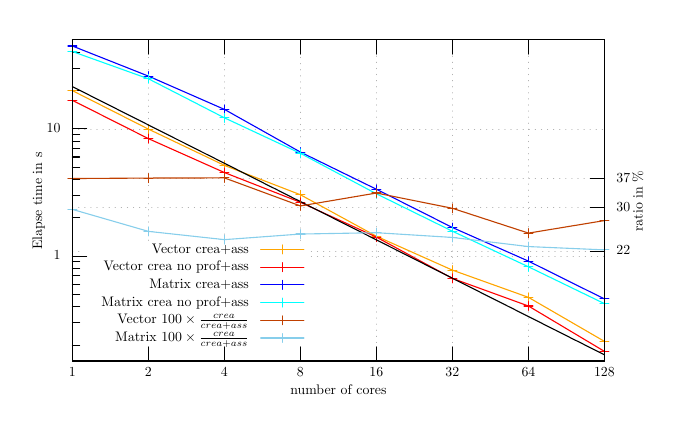
\begin{tikzpicture}[gnuplot]
%% generated with GNUPLOT 6.0p1 (Lua 5.4; terminal rev. Jun 2020, script rev. 118)
%% ven. 10 janv. 2025 17:58:53
\tikzset{every node/.append style={scale=0.50}}
\path (0.000,0.000) rectangle (8.125,4.725);
\gpcolor{color=gp lt color border}
\gpsetlinetype{gp lt border}
\gpsetdashtype{gp dt solid}
\gpsetlinewidth{1.00}
\draw[gp path] (0.568,0.694)--(0.658,0.694);
\draw[gp path] (0.568,0.979)--(0.658,0.979);
\draw[gp path] (0.568,1.181)--(0.658,1.181);
\draw[gp path] (0.568,1.337)--(0.658,1.337);
\draw[gp path] (0.568,1.465)--(0.658,1.465);
\draw[gp path] (0.568,1.573)--(0.658,1.573);
\draw[gp path] (0.568,1.667)--(0.658,1.667);
\draw[gp path] (0.568,1.750)--(0.658,1.750);
\gpcolor{color=gp lt color axes}
\gpsetlinetype{gp lt axes}
\gpsetdashtype{gp dt axes}
\gpsetlinewidth{0.50}
\draw[gp path] (0.568,1.824)--(0.660,1.824);
\draw[gp path] (3.600,1.824)--(7.326,1.824);
\gpcolor{color=gp lt color border}
\gpsetlinetype{gp lt border}
\gpsetdashtype{gp dt solid}
\gpsetlinewidth{1.00}
\draw[gp path] (0.568,1.824)--(0.748,1.824);
\node[gp node right] at (0.476,1.824) {$1$};
\draw[gp path] (0.568,2.310)--(0.658,2.310);
\draw[gp path] (0.568,2.595)--(0.658,2.595);
\draw[gp path] (0.568,2.797)--(0.658,2.797);
\draw[gp path] (0.568,2.954)--(0.658,2.954);
\draw[gp path] (0.568,3.082)--(0.658,3.082);
\draw[gp path] (0.568,3.190)--(0.658,3.190);
\draw[gp path] (0.568,3.284)--(0.658,3.284);
\draw[gp path] (0.568,3.366)--(0.658,3.366);
\gpcolor{color=gp lt color axes}
\gpsetlinetype{gp lt axes}
\gpsetdashtype{gp dt axes}
\gpsetlinewidth{0.50}
\draw[gp path] (0.568,3.440)--(7.326,3.440);
\gpcolor{color=gp lt color border}
\gpsetlinetype{gp lt border}
\gpsetdashtype{gp dt solid}
\gpsetlinewidth{1.00}
\draw[gp path] (0.568,3.440)--(0.748,3.440);
\node[gp node right] at (0.476,3.440) {$10$};
\draw[gp path] (0.568,3.927)--(0.658,3.927);
\draw[gp path] (0.568,4.211)--(0.658,4.211);
\draw[gp path] (0.568,4.413)--(0.658,4.413);
\draw[gp path] (0.568,4.570)--(0.658,4.570);
\gpcolor{color=gp lt color axes}
\gpsetlinetype{gp lt axes}
\gpsetdashtype{gp dt axes}
\gpsetlinewidth{0.50}
\draw[gp path] (0.568,0.492)--(0.568,4.570);
\gpcolor{color=gp lt color border}
\gpsetlinetype{gp lt border}
\gpsetdashtype{gp dt solid}
\gpsetlinewidth{1.00}
\draw[gp path] (0.568,0.492)--(0.568,0.672);
\draw[gp path] (0.568,4.570)--(0.568,4.390);
\node[gp node center] at (0.568,0.338) {1};
\gpcolor{color=gp lt color axes}
\gpsetlinetype{gp lt axes}
\gpsetdashtype{gp dt axes}
\gpsetlinewidth{0.50}
\draw[gp path] (1.533,0.492)--(1.533,0.672);
\draw[gp path] (1.533,2.022)--(1.533,4.570);
\gpcolor{color=gp lt color border}
\gpsetlinetype{gp lt border}
\gpsetdashtype{gp dt solid}
\gpsetlinewidth{1.00}
\draw[gp path] (1.533,0.492)--(1.533,0.672);
\draw[gp path] (1.533,4.570)--(1.533,4.390);
\node[gp node center] at (1.533,0.338) {2};
\gpcolor{color=gp lt color axes}
\gpsetlinetype{gp lt axes}
\gpsetdashtype{gp dt axes}
\gpsetlinewidth{0.50}
\draw[gp path] (2.499,0.492)--(2.499,0.672);
\draw[gp path] (2.499,2.022)--(2.499,4.570);
\gpcolor{color=gp lt color border}
\gpsetlinetype{gp lt border}
\gpsetdashtype{gp dt solid}
\gpsetlinewidth{1.00}
\draw[gp path] (2.499,0.492)--(2.499,0.672);
\draw[gp path] (2.499,4.570)--(2.499,4.390);
\node[gp node center] at (2.499,0.338) {4};
\gpcolor{color=gp lt color axes}
\gpsetlinetype{gp lt axes}
\gpsetdashtype{gp dt axes}
\gpsetlinewidth{0.50}
\draw[gp path] (3.464,0.492)--(3.464,0.672);
\draw[gp path] (3.464,2.022)--(3.464,4.570);
\gpcolor{color=gp lt color border}
\gpsetlinetype{gp lt border}
\gpsetdashtype{gp dt solid}
\gpsetlinewidth{1.00}
\draw[gp path] (3.464,0.492)--(3.464,0.672);
\draw[gp path] (3.464,4.570)--(3.464,4.390);
\node[gp node center] at (3.464,0.338) {8};
\gpcolor{color=gp lt color axes}
\gpsetlinetype{gp lt axes}
\gpsetdashtype{gp dt axes}
\gpsetlinewidth{0.50}
\draw[gp path] (4.429,0.492)--(4.429,4.570);
\gpcolor{color=gp lt color border}
\gpsetlinetype{gp lt border}
\gpsetdashtype{gp dt solid}
\gpsetlinewidth{1.00}
\draw[gp path] (4.429,0.492)--(4.429,0.672);
\draw[gp path] (4.429,4.570)--(4.429,4.390);
\node[gp node center] at (4.429,0.338) {16};
\gpcolor{color=gp lt color axes}
\gpsetlinetype{gp lt axes}
\gpsetdashtype{gp dt axes}
\gpsetlinewidth{0.50}
\draw[gp path] (5.394,0.492)--(5.394,4.570);
\gpcolor{color=gp lt color border}
\gpsetlinetype{gp lt border}
\gpsetdashtype{gp dt solid}
\gpsetlinewidth{1.00}
\draw[gp path] (5.394,0.492)--(5.394,0.672);
\draw[gp path] (5.394,4.570)--(5.394,4.390);
\node[gp node center] at (5.394,0.338) {32};
\gpcolor{color=gp lt color axes}
\gpsetlinetype{gp lt axes}
\gpsetdashtype{gp dt axes}
\gpsetlinewidth{0.50}
\draw[gp path] (6.360,0.492)--(6.360,4.570);
\gpcolor{color=gp lt color border}
\gpsetlinetype{gp lt border}
\gpsetdashtype{gp dt solid}
\gpsetlinewidth{1.00}
\draw[gp path] (6.360,0.492)--(6.360,0.672);
\draw[gp path] (6.360,4.570)--(6.360,4.390);
\node[gp node center] at (6.360,0.338) {64};
\gpcolor{color=gp lt color axes}
\gpsetlinetype{gp lt axes}
\gpsetdashtype{gp dt axes}
\gpsetlinewidth{0.50}
\draw[gp path] (7.325,0.492)--(7.325,4.570);
\gpcolor{color=gp lt color border}
\gpsetlinetype{gp lt border}
\gpsetdashtype{gp dt solid}
\gpsetlinewidth{1.00}
\draw[gp path] (7.325,0.492)--(7.325,0.672);
\draw[gp path] (7.325,4.570)--(7.325,4.390);
\node[gp node center] at (7.325,0.338) {128};
\gpcolor{color=gp lt color axes}
\gpsetlinetype{gp lt axes}
\gpsetdashtype{gp dt axes}
\gpsetlinewidth{0.50}
\draw[gp path] (0.568,1.888)--(0.660,1.888);
\draw[gp path] (3.600,1.888)--(7.326,1.888);
\gpcolor{color=gp lt color border}
\gpsetlinetype{gp lt border}
\gpsetdashtype{gp dt solid}
\gpsetlinewidth{1.00}
\draw[gp path] (7.326,1.888)--(7.146,1.888);
\node[gp node left] at (7.418,1.888) {$22$};
\gpcolor{color=gp lt color axes}
\gpsetlinetype{gp lt axes}
\gpsetdashtype{gp dt axes}
\gpsetlinewidth{0.50}
\draw[gp path] (0.568,2.438)--(7.326,2.438);
\gpcolor{color=gp lt color border}
\gpsetlinetype{gp lt border}
\gpsetdashtype{gp dt solid}
\gpsetlinewidth{1.00}
\draw[gp path] (7.326,2.438)--(7.146,2.438);
\node[gp node left] at (7.418,2.438) {$30$};
\gpcolor{color=gp lt color axes}
\gpsetlinetype{gp lt axes}
\gpsetdashtype{gp dt axes}
\gpsetlinewidth{0.50}
\draw[gp path] (0.568,2.809)--(7.326,2.809);
\gpcolor{color=gp lt color border}
\gpsetlinetype{gp lt border}
\gpsetdashtype{gp dt solid}
\gpsetlinewidth{1.00}
\draw[gp path] (7.326,2.809)--(7.146,2.809);
\node[gp node left] at (7.418,2.809) {$37$};
\draw[gp path] (0.568,4.570)--(0.568,0.492)--(7.326,0.492)--(7.326,4.570)--cycle;
\node[gp node right] at (2.868,1.909) {Vector crea+ass};
\gpcolor{rgb color={1.000,0.647,0.000}}
\draw[gp path] (2.960,1.909)--(3.508,1.909);
\draw[gp path] (0.568,3.925)--(1.533,3.437)--(2.499,2.976)--(3.464,2.603)--(4.429,2.076)%
  --(5.394,1.646)--(6.360,1.300)--(7.325,0.741);
\gpsetpointsize{4.00}
\gp3point{gp mark 1}{}{(0.568,3.925)}
\gp3point{gp mark 1}{}{(1.533,3.437)}
\gp3point{gp mark 1}{}{(2.499,2.976)}
\gp3point{gp mark 1}{}{(3.464,2.603)}
\gp3point{gp mark 1}{}{(4.429,2.076)}
\gp3point{gp mark 1}{}{(5.394,1.646)}
\gp3point{gp mark 1}{}{(6.360,1.300)}
\gp3point{gp mark 1}{}{(7.325,0.741)}
\gp3point{gp mark 1}{}{(3.234,1.909)}
\gpcolor{color=gp lt color border}
\node[gp node right] at (2.868,1.684) {Vector crea no prof+ass };
\gpcolor{rgb color={1.000,0.000,0.000}}
\draw[gp path] (2.960,1.684)--(3.508,1.684);
\draw[gp path] (0.568,3.802)--(1.533,3.316)--(2.499,2.885)--(3.464,2.507)--(4.429,2.065)%
  --(5.394,1.541)--(6.360,1.190)--(7.325,0.614);
\gp3point{gp mark 1}{}{(0.568,3.802)}
\gp3point{gp mark 1}{}{(1.533,3.316)}
\gp3point{gp mark 1}{}{(2.499,2.885)}
\gp3point{gp mark 1}{}{(3.464,2.507)}
\gp3point{gp mark 1}{}{(4.429,2.065)}
\gp3point{gp mark 1}{}{(5.394,1.541)}
\gp3point{gp mark 1}{}{(6.360,1.190)}
\gp3point{gp mark 1}{}{(7.325,0.614)}
\gp3point{gp mark 1}{}{(3.234,1.684)}
\gpcolor{color=gp lt color border}
\node[gp node right] at (2.868,1.459) {Matrix crea+ass};
\gpcolor{rgb color={0.000,0.000,1.000}}
\draw[gp path] (2.960,1.459)--(3.508,1.459);
\draw[gp path] (0.568,4.492)--(1.533,4.110)--(2.499,3.687)--(3.464,3.145)--(4.429,2.673)%
  --(5.394,2.187)--(6.360,1.760)--(7.325,1.280);
\gp3point{gp mark 1}{}{(0.568,4.492)}
\gp3point{gp mark 1}{}{(1.533,4.110)}
\gp3point{gp mark 1}{}{(2.499,3.687)}
\gp3point{gp mark 1}{}{(3.464,3.145)}
\gp3point{gp mark 1}{}{(4.429,2.673)}
\gp3point{gp mark 1}{}{(5.394,2.187)}
\gp3point{gp mark 1}{}{(6.360,1.760)}
\gp3point{gp mark 1}{}{(7.325,1.280)}
\gp3point{gp mark 1}{}{(3.234,1.459)}
\gpcolor{color=gp lt color border}
\node[gp node right] at (2.868,1.234) {Matrix crea no prof+ass};
\gpcolor{rgb color={0.000,1.000,1.000}}
\draw[gp path] (2.960,1.234)--(3.508,1.234);
\draw[gp path] (0.568,4.422)--(1.533,4.076)--(2.499,3.580)--(3.464,3.129)--(4.429,2.615)%
  --(5.394,2.140)--(6.360,1.688)--(7.325,1.220);
\gp3point{gp mark 1}{}{(0.568,4.422)}
\gp3point{gp mark 1}{}{(1.533,4.076)}
\gp3point{gp mark 1}{}{(2.499,3.580)}
\gp3point{gp mark 1}{}{(3.464,3.129)}
\gp3point{gp mark 1}{}{(4.429,2.615)}
\gp3point{gp mark 1}{}{(5.394,2.140)}
\gp3point{gp mark 1}{}{(6.360,1.688)}
\gp3point{gp mark 1}{}{(7.325,1.220)}
\gp3point{gp mark 1}{}{(3.234,1.234)}
\gpcolor{rgb color={0.000,0.000,0.000}}
\draw[gp path] (0.568,3.976)--(0.636,3.942)--(0.705,3.907)--(0.773,3.873)--(0.841,3.838)%
  --(0.909,3.804)--(0.978,3.770)--(1.046,3.735)--(1.114,3.701)--(1.182,3.666)--(1.251,3.632)%
  --(1.319,3.598)--(1.387,3.563)--(1.455,3.529)--(1.524,3.494)--(1.592,3.460)--(1.660,3.426)%
  --(1.728,3.391)--(1.797,3.357)--(1.865,3.322)--(1.933,3.288)--(2.001,3.254)--(2.070,3.219)%
  --(2.138,3.185)--(2.206,3.150)--(2.274,3.116)--(2.343,3.082)--(2.411,3.047)--(2.479,3.013)%
  --(2.547,2.978)--(2.616,2.944)--(2.684,2.909)--(2.752,2.875)--(2.820,2.841)--(2.889,2.806)%
  --(2.957,2.772)--(3.025,2.737)--(3.093,2.703)--(3.162,2.669)--(3.230,2.634)--(3.298,2.600)%
  --(3.366,2.565)--(3.435,2.531)--(3.503,2.497)--(3.571,2.462)--(3.639,2.428)--(3.708,2.393)%
  --(3.776,2.359)--(3.844,2.325)--(3.912,2.290)--(3.981,2.256)--(4.049,2.221)--(4.117,2.187)%
  --(4.185,2.153)--(4.254,2.118)--(4.322,2.084)--(4.390,2.049)--(4.458,2.015)--(4.527,1.981)%
  --(4.595,1.946)--(4.663,1.912)--(4.731,1.877)--(4.800,1.843)--(4.868,1.809)--(4.936,1.774)%
  --(5.004,1.740)--(5.073,1.705)--(5.141,1.671)--(5.209,1.636)--(5.277,1.602)--(5.346,1.568)%
  --(5.414,1.533)--(5.482,1.499)--(5.550,1.464)--(5.619,1.430)--(5.687,1.396)--(5.755,1.361)%
  --(5.823,1.327)--(5.892,1.292)--(5.960,1.258)--(6.028,1.224)--(6.096,1.189)--(6.165,1.155)%
  --(6.233,1.120)--(6.301,1.086)--(6.369,1.052)--(6.438,1.017)--(6.506,0.983)--(6.574,0.948)%
  --(6.642,0.914)--(6.711,0.880)--(6.779,0.845)--(6.847,0.811)--(6.915,0.776)--(6.984,0.742)%
  --(7.052,0.708)--(7.120,0.673)--(7.188,0.639)--(7.257,0.604)--(7.325,0.570);
\gpcolor{color=gp lt color border}
\node[gp node right] at (2.868,1.009) {Vector $100\times\frac{crea}{crea+ass}$};
\gpcolor{rgb color={0.753,0.251,0.000}}
\draw[gp path] (2.960,1.009)--(3.508,1.009);
\draw[gp path] (0.568,2.809)--(1.533,2.815)--(2.499,2.817)--(3.464,2.461)--(4.429,2.625)%
  --(5.394,2.431)--(6.360,2.116)--(7.325,2.275);
\gp3point{gp mark 1}{}{(0.568,2.809)}
\gp3point{gp mark 1}{}{(1.533,2.815)}
\gp3point{gp mark 1}{}{(2.499,2.817)}
\gp3point{gp mark 1}{}{(3.464,2.461)}
\gp3point{gp mark 1}{}{(4.429,2.625)}
\gp3point{gp mark 1}{}{(5.394,2.431)}
\gp3point{gp mark 1}{}{(6.360,2.116)}
\gp3point{gp mark 1}{}{(7.325,2.275)}
\gp3point{gp mark 1}{}{(3.234,1.009)}
\gpcolor{color=gp lt color border}
\node[gp node right] at (2.868,0.784) {Matrix $100\times\frac{crea}{crea+ass}$};
\gpcolor{rgb color={0.529,0.808,0.922}}
\draw[gp path] (2.960,0.784)--(3.508,0.784);
\draw[gp path] (0.568,2.417)--(1.533,2.138)--(2.499,2.033)--(3.464,2.104)--(4.429,2.121)%
  --(5.394,2.061)--(6.360,1.945)--(7.325,1.903);
\gp3point{gp mark 1}{}{(0.568,2.417)}
\gp3point{gp mark 1}{}{(1.533,2.138)}
\gp3point{gp mark 1}{}{(2.499,2.033)}
\gp3point{gp mark 1}{}{(3.464,2.104)}
\gp3point{gp mark 1}{}{(4.429,2.121)}
\gp3point{gp mark 1}{}{(5.394,2.061)}
\gp3point{gp mark 1}{}{(6.360,1.945)}
\gp3point{gp mark 1}{}{(7.325,1.903)}
\gp3point{gp mark 1}{}{(3.234,0.784)}
\gpcolor{color=gp lt color border}
\draw[gp path] (0.568,4.570)--(0.568,0.492)--(7.326,0.492)--(7.326,4.570)--cycle;
\node[gp node center,rotate=-270.0] at (0.146,2.531) {Elapse time in s};
\node[gp node center,rotate=-270.0] at (7.771,2.531) {ratio in \%};
\node[gp node center] at (3.947,0.107) {number of cores};
%% coordinates of the plot area
\gpdefrectangularnode{gp plot 1}{\pgfpoint{0.568cm}{0.492cm}}{\pgfpoint{7.326cm}{4.570cm}}
\end{tikzpicture}
%% gnuplot variables

	\caption{Elementary creation and assembly with \f{} (handmade): Elapsed times in s ( log-log scale)\label{time_ass_f}}
\end{figure}
\begin{figure}
	\subfloat[Strain/stress creation (in s)]{
		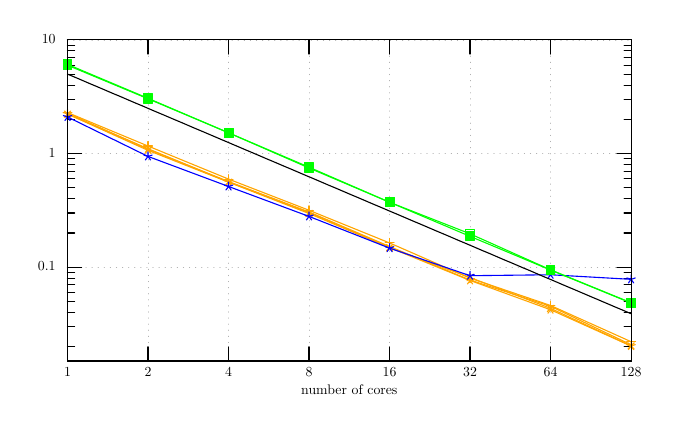
\begin{tikzpicture}[gnuplot]
%% generated with GNUPLOT 6.0p1 (Lua 5.4; terminal rev. Jun 2020, script rev. 118)
%% ven. 10 janv. 2025 17:58:53
\tikzset{every node/.append style={scale=0.50}}
\path (0.000,0.000) rectangle (8.125,4.725);
\gpcolor{color=gp lt color border}
\gpsetlinetype{gp lt border}
\gpsetdashtype{gp dt solid}
\gpsetlinewidth{1.00}
\draw[gp path] (0.506,0.672)--(0.596,0.672);
\draw[gp path] (7.664,0.672)--(7.574,0.672);
\draw[gp path] (0.506,0.927)--(0.596,0.927);
\draw[gp path] (7.664,0.927)--(7.574,0.927);
\draw[gp path] (0.506,1.107)--(0.596,1.107);
\draw[gp path] (7.664,1.107)--(7.574,1.107);
\draw[gp path] (0.506,1.247)--(0.596,1.247);
\draw[gp path] (7.664,1.247)--(7.574,1.247);
\draw[gp path] (0.506,1.361)--(0.596,1.361);
\draw[gp path] (7.664,1.361)--(7.574,1.361);
\draw[gp path] (0.506,1.458)--(0.596,1.458);
\draw[gp path] (7.664,1.458)--(7.574,1.458);
\draw[gp path] (0.506,1.542)--(0.596,1.542);
\draw[gp path] (7.664,1.542)--(7.574,1.542);
\draw[gp path] (0.506,1.616)--(0.596,1.616);
\draw[gp path] (7.664,1.616)--(7.574,1.616);
\gpcolor{color=gp lt color axes}
\gpsetlinetype{gp lt axes}
\gpsetdashtype{gp dt axes}
\gpsetlinewidth{0.50}
\draw[gp path] (0.506,1.682)--(7.664,1.682);
\gpcolor{color=gp lt color border}
\gpsetlinetype{gp lt border}
\gpsetdashtype{gp dt solid}
\gpsetlinewidth{1.00}
\draw[gp path] (0.506,1.682)--(0.686,1.682);
\draw[gp path] (7.664,1.682)--(7.484,1.682);
\node[gp node right] at (0.414,1.682) {$0.1$};
\draw[gp path] (0.506,2.117)--(0.596,2.117);
\draw[gp path] (7.664,2.117)--(7.574,2.117);
\draw[gp path] (0.506,2.371)--(0.596,2.371);
\draw[gp path] (7.664,2.371)--(7.574,2.371);
\draw[gp path] (0.506,2.551)--(0.596,2.551);
\draw[gp path] (7.664,2.551)--(7.574,2.551);
\draw[gp path] (0.506,2.691)--(0.596,2.691);
\draw[gp path] (7.664,2.691)--(7.574,2.691);
\draw[gp path] (0.506,2.806)--(0.596,2.806);
\draw[gp path] (7.664,2.806)--(7.574,2.806);
\draw[gp path] (0.506,2.902)--(0.596,2.902);
\draw[gp path] (7.664,2.902)--(7.574,2.902);
\draw[gp path] (0.506,2.986)--(0.596,2.986);
\draw[gp path] (7.664,2.986)--(7.574,2.986);
\draw[gp path] (0.506,3.060)--(0.596,3.060);
\draw[gp path] (7.664,3.060)--(7.574,3.060);
\gpcolor{color=gp lt color axes}
\gpsetlinetype{gp lt axes}
\gpsetdashtype{gp dt axes}
\gpsetlinewidth{0.50}
\draw[gp path] (0.506,3.126)--(7.664,3.126);
\gpcolor{color=gp lt color border}
\gpsetlinetype{gp lt border}
\gpsetdashtype{gp dt solid}
\gpsetlinewidth{1.00}
\draw[gp path] (0.506,3.126)--(0.686,3.126);
\draw[gp path] (7.664,3.126)--(7.484,3.126);
\node[gp node right] at (0.414,3.126) {$1$};
\draw[gp path] (0.506,3.561)--(0.596,3.561);
\draw[gp path] (7.664,3.561)--(7.574,3.561);
\draw[gp path] (0.506,3.815)--(0.596,3.815);
\draw[gp path] (7.664,3.815)--(7.574,3.815);
\draw[gp path] (0.506,3.995)--(0.596,3.995);
\draw[gp path] (7.664,3.995)--(7.574,3.995);
\draw[gp path] (0.506,4.135)--(0.596,4.135);
\draw[gp path] (7.664,4.135)--(7.574,4.135);
\draw[gp path] (0.506,4.250)--(0.596,4.250);
\draw[gp path] (7.664,4.250)--(7.574,4.250);
\draw[gp path] (0.506,4.346)--(0.596,4.346);
\draw[gp path] (7.664,4.346)--(7.574,4.346);
\draw[gp path] (0.506,4.430)--(0.596,4.430);
\draw[gp path] (7.664,4.430)--(7.574,4.430);
\draw[gp path] (0.506,4.504)--(0.596,4.504);
\draw[gp path] (7.664,4.504)--(7.574,4.504);
\gpcolor{color=gp lt color axes}
\gpsetlinetype{gp lt axes}
\gpsetdashtype{gp dt axes}
\gpsetlinewidth{0.50}
\draw[gp path] (0.506,4.570)--(7.664,4.570);
\gpcolor{color=gp lt color border}
\gpsetlinetype{gp lt border}
\gpsetdashtype{gp dt solid}
\gpsetlinewidth{1.00}
\draw[gp path] (0.506,4.570)--(0.686,4.570);
\draw[gp path] (7.664,4.570)--(7.484,4.570);
\node[gp node right] at (0.414,4.570) {$10$};
\gpcolor{color=gp lt color axes}
\gpsetlinetype{gp lt axes}
\gpsetdashtype{gp dt axes}
\gpsetlinewidth{0.50}
\draw[gp path] (0.506,0.492)--(0.506,4.570);
\gpcolor{color=gp lt color border}
\gpsetlinetype{gp lt border}
\gpsetdashtype{gp dt solid}
\gpsetlinewidth{1.00}
\draw[gp path] (0.506,0.492)--(0.506,0.672);
\draw[gp path] (0.506,4.570)--(0.506,4.390);
\node[gp node center] at (0.506,0.338) {1};
\gpcolor{color=gp lt color axes}
\gpsetlinetype{gp lt axes}
\gpsetdashtype{gp dt axes}
\gpsetlinewidth{0.50}
\draw[gp path] (1.528,0.492)--(1.528,4.570);
\gpcolor{color=gp lt color border}
\gpsetlinetype{gp lt border}
\gpsetdashtype{gp dt solid}
\gpsetlinewidth{1.00}
\draw[gp path] (1.528,0.492)--(1.528,0.672);
\draw[gp path] (1.528,4.570)--(1.528,4.390);
\node[gp node center] at (1.528,0.338) {2};
\gpcolor{color=gp lt color axes}
\gpsetlinetype{gp lt axes}
\gpsetdashtype{gp dt axes}
\gpsetlinewidth{0.50}
\draw[gp path] (2.551,0.492)--(2.551,4.570);
\gpcolor{color=gp lt color border}
\gpsetlinetype{gp lt border}
\gpsetdashtype{gp dt solid}
\gpsetlinewidth{1.00}
\draw[gp path] (2.551,0.492)--(2.551,0.672);
\draw[gp path] (2.551,4.570)--(2.551,4.390);
\node[gp node center] at (2.551,0.338) {4};
\gpcolor{color=gp lt color axes}
\gpsetlinetype{gp lt axes}
\gpsetdashtype{gp dt axes}
\gpsetlinewidth{0.50}
\draw[gp path] (3.573,0.492)--(3.573,4.570);
\gpcolor{color=gp lt color border}
\gpsetlinetype{gp lt border}
\gpsetdashtype{gp dt solid}
\gpsetlinewidth{1.00}
\draw[gp path] (3.573,0.492)--(3.573,0.672);
\draw[gp path] (3.573,4.570)--(3.573,4.390);
\node[gp node center] at (3.573,0.338) {8};
\gpcolor{color=gp lt color axes}
\gpsetlinetype{gp lt axes}
\gpsetdashtype{gp dt axes}
\gpsetlinewidth{0.50}
\draw[gp path] (4.596,0.492)--(4.596,4.570);
\gpcolor{color=gp lt color border}
\gpsetlinetype{gp lt border}
\gpsetdashtype{gp dt solid}
\gpsetlinewidth{1.00}
\draw[gp path] (4.596,0.492)--(4.596,0.672);
\draw[gp path] (4.596,4.570)--(4.596,4.390);
\node[gp node center] at (4.596,0.338) {16};
\gpcolor{color=gp lt color axes}
\gpsetlinetype{gp lt axes}
\gpsetdashtype{gp dt axes}
\gpsetlinewidth{0.50}
\draw[gp path] (5.618,0.492)--(5.618,4.570);
\gpcolor{color=gp lt color border}
\gpsetlinetype{gp lt border}
\gpsetdashtype{gp dt solid}
\gpsetlinewidth{1.00}
\draw[gp path] (5.618,0.492)--(5.618,0.672);
\draw[gp path] (5.618,4.570)--(5.618,4.390);
\node[gp node center] at (5.618,0.338) {32};
\gpcolor{color=gp lt color axes}
\gpsetlinetype{gp lt axes}
\gpsetdashtype{gp dt axes}
\gpsetlinewidth{0.50}
\draw[gp path] (6.640,0.492)--(6.640,4.570);
\gpcolor{color=gp lt color border}
\gpsetlinetype{gp lt border}
\gpsetdashtype{gp dt solid}
\gpsetlinewidth{1.00}
\draw[gp path] (6.640,0.492)--(6.640,0.672);
\draw[gp path] (6.640,4.570)--(6.640,4.390);
\node[gp node center] at (6.640,0.338) {64};
\gpcolor{color=gp lt color axes}
\gpsetlinetype{gp lt axes}
\gpsetdashtype{gp dt axes}
\gpsetlinewidth{0.50}
\draw[gp path] (7.663,0.492)--(7.663,4.570);
\gpcolor{color=gp lt color border}
\gpsetlinetype{gp lt border}
\gpsetdashtype{gp dt solid}
\gpsetlinewidth{1.00}
\draw[gp path] (7.663,0.492)--(7.663,0.672);
\draw[gp path] (7.663,4.570)--(7.663,4.390);
\node[gp node center] at (7.663,0.338) {128};
\draw[gp path] (0.506,4.570)--(0.506,0.492)--(7.664,0.492)--(7.664,4.570)--cycle;
\gpcolor{rgb color={1.000,0.647,0.000}}
\draw[gp path] (0.506,3.647)--(1.528,3.222)--(2.551,2.802)--(3.573,2.406)--(4.596,1.991)%
  --(5.618,1.544)--(6.640,1.197)--(7.663,0.737);
\gpsetpointsize{4.00}
\gp3point{gp mark 1}{}{(0.506,3.647)}
\gp3point{gp mark 1}{}{(1.528,3.222)}
\gp3point{gp mark 1}{}{(2.551,2.802)}
\gp3point{gp mark 1}{}{(3.573,2.406)}
\gp3point{gp mark 1}{}{(4.596,1.991)}
\gp3point{gp mark 1}{}{(5.618,1.544)}
\gp3point{gp mark 1}{}{(6.640,1.197)}
\gp3point{gp mark 1}{}{(7.663,0.737)}
\draw[gp path] (0.506,3.628)--(1.528,3.167)--(2.551,2.763)--(3.573,2.365)--(4.596,1.932)%
  --(5.618,1.552)--(6.640,1.161)--(7.663,0.683);
\gp3point{gp mark 2}{}{(0.506,3.628)}
\gp3point{gp mark 2}{}{(1.528,3.167)}
\gp3point{gp mark 2}{}{(2.551,2.763)}
\gp3point{gp mark 2}{}{(3.573,2.365)}
\gp3point{gp mark 2}{}{(4.596,1.932)}
\gp3point{gp mark 2}{}{(5.618,1.552)}
\gp3point{gp mark 2}{}{(6.640,1.161)}
\gp3point{gp mark 2}{}{(7.663,0.683)}
\draw[gp path] (0.506,3.629)--(1.528,3.188)--(2.551,2.765)--(3.573,2.378)--(4.596,1.932)%
  --(5.618,1.515)--(6.640,1.143)--(7.663,0.682);
\gp3point{gp mark 3}{}{(0.506,3.629)}
\gp3point{gp mark 3}{}{(1.528,3.188)}
\gp3point{gp mark 3}{}{(2.551,2.765)}
\gp3point{gp mark 3}{}{(3.573,2.378)}
\gp3point{gp mark 3}{}{(4.596,1.932)}
\gp3point{gp mark 3}{}{(5.618,1.515)}
\gp3point{gp mark 3}{}{(6.640,1.143)}
\gp3point{gp mark 3}{}{(7.663,0.682)}
\draw[gp path] (0.506,3.640)--(1.528,3.180)--(2.551,2.771)--(3.573,2.384)--(4.596,1.946)%
  --(5.618,1.520)--(6.640,1.187)--(7.663,0.698);
\gp3point{gp mark 0}{}{(0.506,3.640)}
\gp3point{gp mark 0}{}{(1.528,3.180)}
\gp3point{gp mark 0}{}{(2.551,2.771)}
\gp3point{gp mark 0}{}{(3.573,2.384)}
\gp3point{gp mark 0}{}{(4.596,1.946)}
\gp3point{gp mark 0}{}{(5.618,1.520)}
\gp3point{gp mark 0}{}{(6.640,1.187)}
\gp3point{gp mark 0}{}{(7.663,0.698)}
\gpcolor{rgb color={0.000,0.000,1.000}}
\draw[gp path] (0.506,3.591)--(1.528,3.090)--(2.551,2.708)--(3.573,2.328)--(4.596,1.925)%
  --(5.618,1.575)--(6.640,1.587)--(7.663,1.529);
\gp3point{gp mark 3}{}{(0.506,3.591)}
\gp3point{gp mark 3}{}{(1.528,3.090)}
\gp3point{gp mark 3}{}{(2.551,2.708)}
\gp3point{gp mark 3}{}{(3.573,2.328)}
\gp3point{gp mark 3}{}{(4.596,1.925)}
\gp3point{gp mark 3}{}{(5.618,1.575)}
\gp3point{gp mark 3}{}{(6.640,1.587)}
\gp3point{gp mark 3}{}{(7.663,1.529)}
\gpcolor{rgb color={0.000,1.000,0.000}}
\draw[gp path] (0.506,4.259)--(1.528,3.828)--(2.551,3.390)--(3.573,2.943)--(4.596,2.508)%
  --(5.618,2.107)--(6.640,1.650)--(7.663,1.232);
\gp3point{gp mark 4}{}{(0.506,4.259)}
\gp3point{gp mark 4}{}{(1.528,3.828)}
\gp3point{gp mark 4}{}{(2.551,3.390)}
\gp3point{gp mark 4}{}{(3.573,2.943)}
\gp3point{gp mark 4}{}{(4.596,2.508)}
\gp3point{gp mark 4}{}{(5.618,2.107)}
\gp3point{gp mark 4}{}{(6.640,1.650)}
\gp3point{gp mark 4}{}{(7.663,1.232)}
\draw[gp path] (0.506,4.248)--(1.528,3.822)--(2.551,3.390)--(3.573,2.953)--(4.596,2.508)%
  --(5.618,2.075)--(6.640,1.647)--(7.663,1.228);
\gp3point{gp mark 5}{}{(0.506,4.248)}
\gp3point{gp mark 5}{}{(1.528,3.822)}
\gp3point{gp mark 5}{}{(2.551,3.390)}
\gp3point{gp mark 5}{}{(3.573,2.953)}
\gp3point{gp mark 5}{}{(4.596,2.508)}
\gp3point{gp mark 5}{}{(5.618,2.075)}
\gp3point{gp mark 5}{}{(6.640,1.647)}
\gp3point{gp mark 5}{}{(7.663,1.228)}
\gpcolor{rgb color={0.000,0.000,0.000}}
\draw[gp path] (0.506,4.135)--(0.578,4.105)--(0.651,4.074)--(0.723,4.043)--(0.795,4.012)%
  --(0.867,3.982)--(0.940,3.951)--(1.012,3.920)--(1.084,3.889)--(1.157,3.859)--(1.229,3.828)%
  --(1.301,3.797)--(1.373,3.766)--(1.446,3.736)--(1.518,3.705)--(1.590,3.674)--(1.663,3.643)%
  --(1.735,3.613)--(1.807,3.582)--(1.880,3.551)--(1.952,3.521)--(2.024,3.490)--(2.096,3.459)%
  --(2.169,3.428)--(2.241,3.398)--(2.313,3.367)--(2.386,3.336)--(2.458,3.305)--(2.530,3.275)%
  --(2.602,3.244)--(2.675,3.213)--(2.747,3.182)--(2.819,3.152)--(2.892,3.121)--(2.964,3.090)%
  --(3.036,3.059)--(3.108,3.029)--(3.181,2.998)--(3.253,2.967)--(3.325,2.937)--(3.398,2.906)%
  --(3.470,2.875)--(3.542,2.844)--(3.615,2.814)--(3.687,2.783)--(3.759,2.752)--(3.831,2.721)%
  --(3.904,2.691)--(3.976,2.660)--(4.048,2.629)--(4.121,2.598)--(4.193,2.568)--(4.265,2.537)%
  --(4.337,2.506)--(4.410,2.475)--(4.482,2.445)--(4.554,2.414)--(4.627,2.383)--(4.699,2.353)%
  --(4.771,2.322)--(4.843,2.291)--(4.916,2.260)--(4.988,2.230)--(5.060,2.199)--(5.133,2.168)%
  --(5.205,2.137)--(5.277,2.107)--(5.350,2.076)--(5.422,2.045)--(5.494,2.014)--(5.566,1.984)%
  --(5.639,1.953)--(5.711,1.922)--(5.783,1.891)--(5.856,1.861)--(5.928,1.830)--(6.000,1.799)%
  --(6.072,1.768)--(6.145,1.738)--(6.217,1.707)--(6.289,1.676)--(6.362,1.646)--(6.434,1.615)%
  --(6.506,1.584)--(6.578,1.553)--(6.651,1.523)--(6.723,1.492)--(6.795,1.461)--(6.868,1.430)%
  --(6.940,1.400)--(7.012,1.369)--(7.085,1.338)--(7.157,1.307)--(7.229,1.277)--(7.301,1.246)%
  --(7.374,1.215)--(7.446,1.184)--(7.518,1.154)--(7.591,1.123)--(7.663,1.092);
\gpcolor{color=gp lt color border}
\draw[gp path] (0.506,4.570)--(0.506,0.492)--(7.664,0.492)--(7.664,4.570)--cycle;
\node[gp node center] at (4.085,0.107) {number of cores};
%% coordinates of the plot area
\gpdefrectangularnode{gp plot 1}{\pgfpoint{0.506cm}{0.492cm}}{\pgfpoint{7.664cm}{4.570cm}}
\end{tikzpicture}
%% gnuplot variables

	}
	\subfloat[Strain/stress creation (Ratio vs MFEM)]{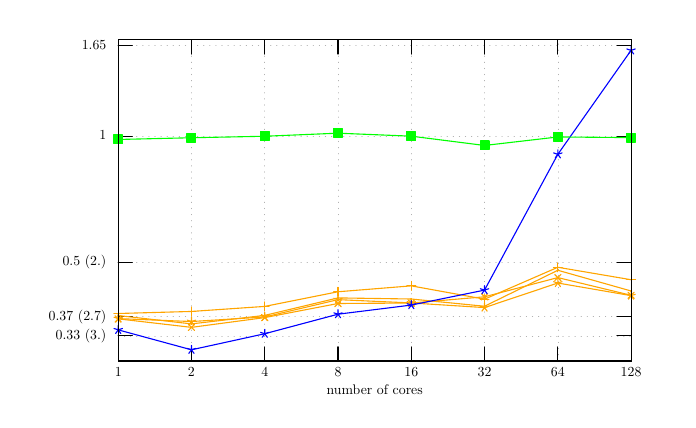
\begin{tikzpicture}[gnuplot]
%% generated with GNUPLOT 6.0p1 (Lua 5.4; terminal rev. Jun 2020, script rev. 118)
%% ven. 10 janv. 2025 17:58:53
\tikzset{every node/.append style={scale=0.50}}
\path (0.000,0.000) rectangle (8.125,4.725);
\gpcolor{color=gp lt color axes}
\gpsetlinetype{gp lt axes}
\gpsetdashtype{gp dt axes}
\gpsetlinewidth{0.50}
\draw[gp path] (1.150,0.811)--(7.664,0.811);
\gpcolor{color=gp lt color border}
\gpsetlinetype{gp lt border}
\gpsetdashtype{gp dt solid}
\gpsetlinewidth{1.00}
\draw[gp path] (1.150,0.811)--(1.330,0.811);
\draw[gp path] (7.664,0.811)--(7.484,0.811);
\node[gp node right] at (1.058,0.811) {0.33 (3.)};
\gpcolor{color=gp lt color axes}
\gpsetlinetype{gp lt axes}
\gpsetdashtype{gp dt axes}
\gpsetlinewidth{0.50}
\draw[gp path] (1.150,1.054)--(7.664,1.054);
\gpcolor{color=gp lt color border}
\gpsetlinetype{gp lt border}
\gpsetdashtype{gp dt solid}
\gpsetlinewidth{1.00}
\draw[gp path] (1.150,1.054)--(1.330,1.054);
\draw[gp path] (7.664,1.054)--(7.484,1.054);
\node[gp node right] at (1.058,1.054) {0.37 (2.7)};
\gpcolor{color=gp lt color axes}
\gpsetlinetype{gp lt axes}
\gpsetdashtype{gp dt axes}
\gpsetlinewidth{0.50}
\draw[gp path] (1.150,1.748)--(7.664,1.748);
\gpcolor{color=gp lt color border}
\gpsetlinetype{gp lt border}
\gpsetdashtype{gp dt solid}
\gpsetlinewidth{1.00}
\draw[gp path] (1.150,1.748)--(1.330,1.748);
\draw[gp path] (7.664,1.748)--(7.484,1.748);
\node[gp node right] at (1.058,1.748) {0.5 (2.)};
\gpcolor{color=gp lt color axes}
\gpsetlinetype{gp lt axes}
\gpsetdashtype{gp dt axes}
\gpsetlinewidth{0.50}
\draw[gp path] (1.150,3.346)--(7.664,3.346);
\gpcolor{color=gp lt color border}
\gpsetlinetype{gp lt border}
\gpsetdashtype{gp dt solid}
\gpsetlinewidth{1.00}
\draw[gp path] (1.150,3.346)--(1.330,3.346);
\draw[gp path] (7.664,3.346)--(7.484,3.346);
\node[gp node right] at (1.058,3.346) {$1$};
\gpcolor{color=gp lt color axes}
\gpsetlinetype{gp lt axes}
\gpsetdashtype{gp dt axes}
\gpsetlinewidth{0.50}
\draw[gp path] (1.150,4.501)--(7.664,4.501);
\gpcolor{color=gp lt color border}
\gpsetlinetype{gp lt border}
\gpsetdashtype{gp dt solid}
\gpsetlinewidth{1.00}
\draw[gp path] (1.150,4.501)--(1.330,4.501);
\draw[gp path] (7.664,4.501)--(7.484,4.501);
\node[gp node right] at (1.058,4.501) {$1.65$};
\gpcolor{color=gp lt color axes}
\gpsetlinetype{gp lt axes}
\gpsetdashtype{gp dt axes}
\gpsetlinewidth{0.50}
\draw[gp path] (1.150,0.492)--(1.150,4.570);
\gpcolor{color=gp lt color border}
\gpsetlinetype{gp lt border}
\gpsetdashtype{gp dt solid}
\gpsetlinewidth{1.00}
\draw[gp path] (1.150,0.492)--(1.150,0.672);
\draw[gp path] (1.150,4.570)--(1.150,4.390);
\node[gp node center] at (1.150,0.338) {1};
\gpcolor{color=gp lt color axes}
\gpsetlinetype{gp lt axes}
\gpsetdashtype{gp dt axes}
\gpsetlinewidth{0.50}
\draw[gp path] (2.080,0.492)--(2.080,4.570);
\gpcolor{color=gp lt color border}
\gpsetlinetype{gp lt border}
\gpsetdashtype{gp dt solid}
\gpsetlinewidth{1.00}
\draw[gp path] (2.080,0.492)--(2.080,0.672);
\draw[gp path] (2.080,4.570)--(2.080,4.390);
\node[gp node center] at (2.080,0.338) {2};
\gpcolor{color=gp lt color axes}
\gpsetlinetype{gp lt axes}
\gpsetdashtype{gp dt axes}
\gpsetlinewidth{0.50}
\draw[gp path] (3.011,0.492)--(3.011,4.570);
\gpcolor{color=gp lt color border}
\gpsetlinetype{gp lt border}
\gpsetdashtype{gp dt solid}
\gpsetlinewidth{1.00}
\draw[gp path] (3.011,0.492)--(3.011,0.672);
\draw[gp path] (3.011,4.570)--(3.011,4.390);
\node[gp node center] at (3.011,0.338) {4};
\gpcolor{color=gp lt color axes}
\gpsetlinetype{gp lt axes}
\gpsetdashtype{gp dt axes}
\gpsetlinewidth{0.50}
\draw[gp path] (3.941,0.492)--(3.941,4.570);
\gpcolor{color=gp lt color border}
\gpsetlinetype{gp lt border}
\gpsetdashtype{gp dt solid}
\gpsetlinewidth{1.00}
\draw[gp path] (3.941,0.492)--(3.941,0.672);
\draw[gp path] (3.941,4.570)--(3.941,4.390);
\node[gp node center] at (3.941,0.338) {8};
\gpcolor{color=gp lt color axes}
\gpsetlinetype{gp lt axes}
\gpsetdashtype{gp dt axes}
\gpsetlinewidth{0.50}
\draw[gp path] (4.872,0.492)--(4.872,4.570);
\gpcolor{color=gp lt color border}
\gpsetlinetype{gp lt border}
\gpsetdashtype{gp dt solid}
\gpsetlinewidth{1.00}
\draw[gp path] (4.872,0.492)--(4.872,0.672);
\draw[gp path] (4.872,4.570)--(4.872,4.390);
\node[gp node center] at (4.872,0.338) {16};
\gpcolor{color=gp lt color axes}
\gpsetlinetype{gp lt axes}
\gpsetdashtype{gp dt axes}
\gpsetlinewidth{0.50}
\draw[gp path] (5.802,0.492)--(5.802,4.570);
\gpcolor{color=gp lt color border}
\gpsetlinetype{gp lt border}
\gpsetdashtype{gp dt solid}
\gpsetlinewidth{1.00}
\draw[gp path] (5.802,0.492)--(5.802,0.672);
\draw[gp path] (5.802,4.570)--(5.802,4.390);
\node[gp node center] at (5.802,0.338) {32};
\gpcolor{color=gp lt color axes}
\gpsetlinetype{gp lt axes}
\gpsetdashtype{gp dt axes}
\gpsetlinewidth{0.50}
\draw[gp path] (6.733,0.492)--(6.733,4.570);
\gpcolor{color=gp lt color border}
\gpsetlinetype{gp lt border}
\gpsetdashtype{gp dt solid}
\gpsetlinewidth{1.00}
\draw[gp path] (6.733,0.492)--(6.733,0.672);
\draw[gp path] (6.733,4.570)--(6.733,4.390);
\node[gp node center] at (6.733,0.338) {64};
\gpcolor{color=gp lt color axes}
\gpsetlinetype{gp lt axes}
\gpsetdashtype{gp dt axes}
\gpsetlinewidth{0.50}
\draw[gp path] (7.663,0.492)--(7.663,4.570);
\gpcolor{color=gp lt color border}
\gpsetlinetype{gp lt border}
\gpsetdashtype{gp dt solid}
\gpsetlinewidth{1.00}
\draw[gp path] (7.663,0.492)--(7.663,0.672);
\draw[gp path] (7.663,4.570)--(7.663,4.390);
\node[gp node center] at (7.663,0.338) {128};
\draw[gp path] (1.150,4.570)--(1.150,0.492)--(7.664,0.492)--(7.664,4.570)--cycle;
\gpcolor{rgb color={1.000,0.647,0.000}}
\draw[gp path] (1.150,1.095)--(2.080,1.121)--(3.011,1.185)--(3.941,1.371)--(4.872,1.446)%
  --(5.802,1.277)--(6.733,1.682)--(7.663,1.524);
\gpsetpointsize{4.00}
\gp3point{gp mark 1}{}{(1.150,1.095)}
\gp3point{gp mark 1}{}{(2.080,1.121)}
\gp3point{gp mark 1}{}{(3.011,1.185)}
\gp3point{gp mark 1}{}{(3.941,1.371)}
\gp3point{gp mark 1}{}{(4.872,1.446)}
\gp3point{gp mark 1}{}{(5.802,1.277)}
\gp3point{gp mark 1}{}{(6.733,1.682)}
\gp3point{gp mark 1}{}{(7.663,1.524)}
\draw[gp path] (1.150,1.027)--(2.080,0.919)--(3.011,1.043)--(3.941,1.222)--(4.872,1.228)%
  --(5.802,1.307)--(6.733,1.551)--(7.663,1.326);
\gp3point{gp mark 2}{}{(1.150,1.027)}
\gp3point{gp mark 2}{}{(2.080,0.919)}
\gp3point{gp mark 2}{}{(3.011,1.043)}
\gp3point{gp mark 2}{}{(3.941,1.222)}
\gp3point{gp mark 2}{}{(4.872,1.228)}
\gp3point{gp mark 2}{}{(5.802,1.307)}
\gp3point{gp mark 2}{}{(6.733,1.551)}
\gp3point{gp mark 2}{}{(7.663,1.326)}
\draw[gp path] (1.150,1.030)--(2.080,0.993)--(3.011,1.051)--(3.941,1.271)--(4.872,1.229)%
  --(5.802,1.170)--(6.733,1.482)--(7.663,1.322);
\gp3point{gp mark 3}{}{(1.150,1.030)}
\gp3point{gp mark 3}{}{(2.080,0.993)}
\gp3point{gp mark 3}{}{(3.011,1.051)}
\gp3point{gp mark 3}{}{(3.941,1.271)}
\gp3point{gp mark 3}{}{(4.872,1.229)}
\gp3point{gp mark 3}{}{(5.802,1.170)}
\gp3point{gp mark 3}{}{(6.733,1.482)}
\gp3point{gp mark 3}{}{(7.663,1.322)}
\draw[gp path] (1.150,1.069)--(2.080,0.963)--(3.011,1.071)--(3.941,1.293)--(4.872,1.279)%
  --(5.802,1.187)--(6.733,1.644)--(7.663,1.381);
\gp3point{gp mark 0}{}{(1.150,1.069)}
\gp3point{gp mark 0}{}{(2.080,0.963)}
\gp3point{gp mark 0}{}{(3.011,1.071)}
\gp3point{gp mark 0}{}{(3.941,1.293)}
\gp3point{gp mark 0}{}{(4.872,1.279)}
\gp3point{gp mark 0}{}{(5.802,1.187)}
\gp3point{gp mark 0}{}{(6.733,1.644)}
\gp3point{gp mark 0}{}{(7.663,1.381)}
\gpcolor{rgb color={0.000,0.000,1.000}}
\draw[gp path] (1.150,0.887)--(2.080,0.634)--(3.011,0.838)--(3.941,1.086)--(4.872,1.202)%
  --(5.802,1.392)--(6.733,3.117)--(7.663,4.437);
\gp3point{gp mark 3}{}{(1.150,0.887)}
\gp3point{gp mark 3}{}{(2.080,0.634)}
\gp3point{gp mark 3}{}{(3.011,0.838)}
\gp3point{gp mark 3}{}{(3.941,1.086)}
\gp3point{gp mark 3}{}{(4.872,1.202)}
\gp3point{gp mark 3}{}{(5.802,1.392)}
\gp3point{gp mark 3}{}{(6.733,3.117)}
\gp3point{gp mark 3}{}{(7.663,4.437)}
\gpcolor{rgb color={0.000,1.000,0.000}}
\draw[gp path] (1.150,3.305)--(2.080,3.327)--(3.011,3.346)--(3.941,3.385)--(4.872,3.347)%
  --(5.802,3.229)--(6.733,3.337)--(7.663,3.329);
\gp3point{gp mark 5}{}{(1.150,3.305)}
\gp3point{gp mark 5}{}{(2.080,3.327)}
\gp3point{gp mark 5}{}{(3.011,3.346)}
\gp3point{gp mark 5}{}{(3.941,3.385)}
\gp3point{gp mark 5}{}{(4.872,3.347)}
\gp3point{gp mark 5}{}{(5.802,3.229)}
\gp3point{gp mark 5}{}{(6.733,3.337)}
\gp3point{gp mark 5}{}{(7.663,3.329)}
\gpcolor{color=gp lt color border}
\draw[gp path] (1.150,4.570)--(1.150,0.492)--(7.664,0.492)--(7.664,4.570)--cycle;
\node[gp node center] at (4.407,0.107) {number of cores};
%% coordinates of the plot area
\gpdefrectangularnode{gp plot 1}{\pgfpoint{1.150cm}{0.492cm}}{\pgfpoint{7.664cm}{4.570cm}}
\end{tikzpicture}
%% gnuplot variables
}\\
	\subfloat[One non-linear loop iteration (in s)]{
		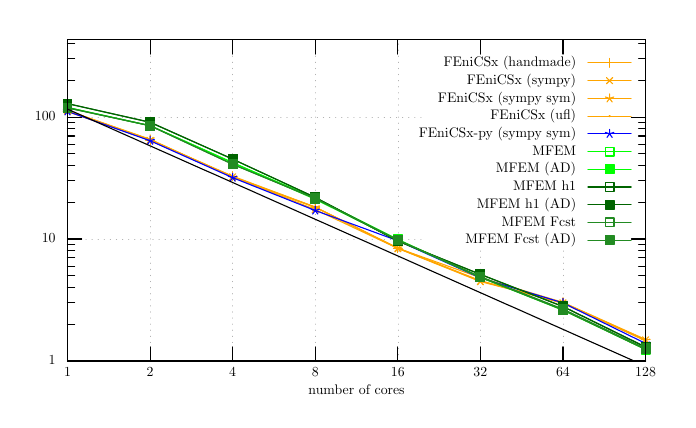
\begin{tikzpicture}[gnuplot]
%% generated with GNUPLOT 6.0p1 (Lua 5.4; terminal rev. Jun 2020, script rev. 118)
%% ven. 10 janv. 2025 17:58:53
\tikzset{every node/.append style={scale=0.50}}
\path (0.000,0.000) rectangle (8.125,4.725);
\gpcolor{color=gp lt color axes}
\gpsetlinetype{gp lt axes}
\gpsetdashtype{gp dt axes}
\gpsetlinewidth{0.50}
\draw[gp path] (0.506,0.492)--(7.848,0.492);
\gpcolor{color=gp lt color border}
\gpsetlinetype{gp lt border}
\gpsetdashtype{gp dt solid}
\gpsetlinewidth{1.00}
\draw[gp path] (0.506,0.492)--(0.686,0.492);
\draw[gp path] (7.848,0.492)--(7.668,0.492);
\node[gp node right] at (0.414,0.492) {$1$};
\draw[gp path] (0.506,0.958)--(0.596,0.958);
\draw[gp path] (7.848,0.958)--(7.758,0.958);
\draw[gp path] (0.506,1.231)--(0.596,1.231);
\draw[gp path] (7.848,1.231)--(7.758,1.231);
\draw[gp path] (0.506,1.424)--(0.596,1.424);
\draw[gp path] (7.848,1.424)--(7.758,1.424);
\draw[gp path] (0.506,1.574)--(0.596,1.574);
\draw[gp path] (7.848,1.574)--(7.758,1.574);
\draw[gp path] (0.506,1.697)--(0.596,1.697);
\draw[gp path] (7.848,1.697)--(7.758,1.697);
\draw[gp path] (0.506,1.801)--(0.596,1.801);
\draw[gp path] (7.848,1.801)--(7.758,1.801);
\draw[gp path] (0.506,1.890)--(0.596,1.890);
\draw[gp path] (7.848,1.890)--(7.758,1.890);
\draw[gp path] (0.506,1.970)--(0.596,1.970);
\draw[gp path] (7.848,1.970)--(7.758,1.970);
\gpcolor{color=gp lt color axes}
\gpsetlinetype{gp lt axes}
\gpsetdashtype{gp dt axes}
\gpsetlinewidth{0.50}
\draw[gp path] (0.506,2.041)--(5.000,2.041);
\draw[gp path] (7.756,2.041)--(7.848,2.041);
\gpcolor{color=gp lt color border}
\gpsetlinetype{gp lt border}
\gpsetdashtype{gp dt solid}
\gpsetlinewidth{1.00}
\draw[gp path] (0.506,2.041)--(0.686,2.041);
\draw[gp path] (7.848,2.041)--(7.668,2.041);
\node[gp node right] at (0.414,2.041) {$10$};
\draw[gp path] (0.506,2.507)--(0.596,2.507);
\draw[gp path] (7.848,2.507)--(7.758,2.507);
\draw[gp path] (0.506,2.779)--(0.596,2.779);
\draw[gp path] (7.848,2.779)--(7.758,2.779);
\draw[gp path] (0.506,2.973)--(0.596,2.973);
\draw[gp path] (7.848,2.973)--(7.758,2.973);
\draw[gp path] (0.506,3.123)--(0.596,3.123);
\draw[gp path] (7.848,3.123)--(7.758,3.123);
\draw[gp path] (0.506,3.246)--(0.596,3.246);
\draw[gp path] (7.848,3.246)--(7.758,3.246);
\draw[gp path] (0.506,3.349)--(0.596,3.349);
\draw[gp path] (7.848,3.349)--(7.758,3.349);
\draw[gp path] (0.506,3.439)--(0.596,3.439);
\draw[gp path] (7.848,3.439)--(7.758,3.439);
\draw[gp path] (0.506,3.518)--(0.596,3.518);
\draw[gp path] (7.848,3.518)--(7.758,3.518);
\gpcolor{color=gp lt color axes}
\gpsetlinetype{gp lt axes}
\gpsetdashtype{gp dt axes}
\gpsetlinewidth{0.50}
\draw[gp path] (0.506,3.589)--(5.000,3.589);
\draw[gp path] (7.756,3.589)--(7.848,3.589);
\gpcolor{color=gp lt color border}
\gpsetlinetype{gp lt border}
\gpsetdashtype{gp dt solid}
\gpsetlinewidth{1.00}
\draw[gp path] (0.506,3.589)--(0.686,3.589);
\draw[gp path] (7.848,3.589)--(7.668,3.589);
\node[gp node right] at (0.414,3.589) {$100$};
\draw[gp path] (0.506,4.055)--(0.596,4.055);
\draw[gp path] (7.848,4.055)--(7.758,4.055);
\draw[gp path] (0.506,4.328)--(0.596,4.328);
\draw[gp path] (7.848,4.328)--(7.758,4.328);
\draw[gp path] (0.506,4.521)--(0.596,4.521);
\draw[gp path] (7.848,4.521)--(7.758,4.521);
\gpcolor{color=gp lt color axes}
\gpsetlinetype{gp lt axes}
\gpsetdashtype{gp dt axes}
\gpsetlinewidth{0.50}
\draw[gp path] (0.506,0.492)--(0.506,4.570);
\gpcolor{color=gp lt color border}
\gpsetlinetype{gp lt border}
\gpsetdashtype{gp dt solid}
\gpsetlinewidth{1.00}
\draw[gp path] (0.506,0.492)--(0.506,0.672);
\draw[gp path] (0.506,4.570)--(0.506,4.390);
\node[gp node center] at (0.506,0.338) {1};
\gpcolor{color=gp lt color axes}
\gpsetlinetype{gp lt axes}
\gpsetdashtype{gp dt axes}
\gpsetlinewidth{0.50}
\draw[gp path] (1.555,0.492)--(1.555,4.570);
\gpcolor{color=gp lt color border}
\gpsetlinetype{gp lt border}
\gpsetdashtype{gp dt solid}
\gpsetlinewidth{1.00}
\draw[gp path] (1.555,0.492)--(1.555,0.672);
\draw[gp path] (1.555,4.570)--(1.555,4.390);
\node[gp node center] at (1.555,0.338) {2};
\gpcolor{color=gp lt color axes}
\gpsetlinetype{gp lt axes}
\gpsetdashtype{gp dt axes}
\gpsetlinewidth{0.50}
\draw[gp path] (2.603,0.492)--(2.603,4.570);
\gpcolor{color=gp lt color border}
\gpsetlinetype{gp lt border}
\gpsetdashtype{gp dt solid}
\gpsetlinewidth{1.00}
\draw[gp path] (2.603,0.492)--(2.603,0.672);
\draw[gp path] (2.603,4.570)--(2.603,4.390);
\node[gp node center] at (2.603,0.338) {4};
\gpcolor{color=gp lt color axes}
\gpsetlinetype{gp lt axes}
\gpsetdashtype{gp dt axes}
\gpsetlinewidth{0.50}
\draw[gp path] (3.652,0.492)--(3.652,4.570);
\gpcolor{color=gp lt color border}
\gpsetlinetype{gp lt border}
\gpsetdashtype{gp dt solid}
\gpsetlinewidth{1.00}
\draw[gp path] (3.652,0.492)--(3.652,0.672);
\draw[gp path] (3.652,4.570)--(3.652,4.390);
\node[gp node center] at (3.652,0.338) {8};
\gpcolor{color=gp lt color axes}
\gpsetlinetype{gp lt axes}
\gpsetdashtype{gp dt axes}
\gpsetlinewidth{0.50}
\draw[gp path] (4.701,0.492)--(4.701,4.570);
\gpcolor{color=gp lt color border}
\gpsetlinetype{gp lt border}
\gpsetdashtype{gp dt solid}
\gpsetlinewidth{1.00}
\draw[gp path] (4.701,0.492)--(4.701,0.672);
\draw[gp path] (4.701,4.570)--(4.701,4.390);
\node[gp node center] at (4.701,0.338) {16};
\gpcolor{color=gp lt color axes}
\gpsetlinetype{gp lt axes}
\gpsetdashtype{gp dt axes}
\gpsetlinewidth{0.50}
\draw[gp path] (5.749,0.492)--(5.749,1.915);
\draw[gp path] (5.749,4.390)--(5.749,4.570);
\gpcolor{color=gp lt color border}
\gpsetlinetype{gp lt border}
\gpsetdashtype{gp dt solid}
\gpsetlinewidth{1.00}
\draw[gp path] (5.749,0.492)--(5.749,0.672);
\draw[gp path] (5.749,4.570)--(5.749,4.390);
\node[gp node center] at (5.749,0.338) {32};
\gpcolor{color=gp lt color axes}
\gpsetlinetype{gp lt axes}
\gpsetdashtype{gp dt axes}
\gpsetlinewidth{0.50}
\draw[gp path] (6.798,0.492)--(6.798,1.915);
\draw[gp path] (6.798,4.390)--(6.798,4.570);
\gpcolor{color=gp lt color border}
\gpsetlinetype{gp lt border}
\gpsetdashtype{gp dt solid}
\gpsetlinewidth{1.00}
\draw[gp path] (6.798,0.492)--(6.798,0.672);
\draw[gp path] (6.798,4.570)--(6.798,4.390);
\node[gp node center] at (6.798,0.338) {64};
\gpcolor{color=gp lt color axes}
\gpsetlinetype{gp lt axes}
\gpsetdashtype{gp dt axes}
\gpsetlinewidth{0.50}
\draw[gp path] (7.847,0.492)--(7.847,4.570);
\gpcolor{color=gp lt color border}
\gpsetlinetype{gp lt border}
\gpsetdashtype{gp dt solid}
\gpsetlinewidth{1.00}
\draw[gp path] (7.847,0.492)--(7.847,0.672);
\draw[gp path] (7.847,4.570)--(7.847,4.390);
\node[gp node center] at (7.847,0.338) {128};
\draw[gp path] (0.506,4.570)--(0.506,0.492)--(7.848,0.492)--(7.848,4.570)--cycle;
\node[gp node right] at (7.024,4.277) {FEniCSx (handmade)};
\gpcolor{rgb color={1.000,0.647,0.000}}
\draw[gp path] (7.116,4.277)--(7.664,4.277);
\draw[gp path] (0.506,3.659)--(1.555,3.297)--(2.603,2.839)--(3.652,2.447)--(4.701,1.924)%
  --(5.749,1.550)--(6.798,1.236)--(7.847,0.765);
\gpsetpointsize{4.00}
\gp3point{gp mark 1}{}{(0.506,3.659)}
\gp3point{gp mark 1}{}{(1.555,3.297)}
\gp3point{gp mark 1}{}{(2.603,2.839)}
\gp3point{gp mark 1}{}{(3.652,2.447)}
\gp3point{gp mark 1}{}{(4.701,1.924)}
\gp3point{gp mark 1}{}{(5.749,1.550)}
\gp3point{gp mark 1}{}{(6.798,1.236)}
\gp3point{gp mark 1}{}{(7.847,0.765)}
\gp3point{gp mark 1}{}{(7.390,4.277)}
\gpcolor{color=gp lt color border}
\node[gp node right] at (7.024,4.052) {FEniCSx (sympy)};
\gpcolor{rgb color={1.000,0.647,0.000}}
\draw[gp path] (7.116,4.052)--(7.664,4.052);
\draw[gp path] (0.506,3.671)--(1.555,3.293)--(2.603,2.831)--(3.652,2.415)--(4.701,1.922)%
  --(5.749,1.501)--(6.798,1.231)--(7.847,0.760);
\gp3point{gp mark 2}{}{(0.506,3.671)}
\gp3point{gp mark 2}{}{(1.555,3.293)}
\gp3point{gp mark 2}{}{(2.603,2.831)}
\gp3point{gp mark 2}{}{(3.652,2.415)}
\gp3point{gp mark 2}{}{(4.701,1.922)}
\gp3point{gp mark 2}{}{(5.749,1.501)}
\gp3point{gp mark 2}{}{(6.798,1.231)}
\gp3point{gp mark 2}{}{(7.847,0.760)}
\gp3point{gp mark 2}{}{(7.390,4.052)}
\gpcolor{color=gp lt color border}
\node[gp node right] at (7.024,3.827) {FEniCSx (sympy sym)};
\gpcolor{rgb color={1.000,0.647,0.000}}
\draw[gp path] (7.116,3.827)--(7.664,3.827);
\draw[gp path] (0.506,3.669)--(1.555,3.308)--(2.603,2.824)--(3.652,2.444)--(4.701,1.924)%
  --(5.749,1.507)--(6.798,1.234)--(7.847,0.752);
\gp3point{gp mark 3}{}{(0.506,3.669)}
\gp3point{gp mark 3}{}{(1.555,3.308)}
\gp3point{gp mark 3}{}{(2.603,2.824)}
\gp3point{gp mark 3}{}{(3.652,2.444)}
\gp3point{gp mark 3}{}{(4.701,1.924)}
\gp3point{gp mark 3}{}{(5.749,1.507)}
\gp3point{gp mark 3}{}{(6.798,1.234)}
\gp3point{gp mark 3}{}{(7.847,0.752)}
\gp3point{gp mark 3}{}{(7.390,3.827)}
\gpcolor{color=gp lt color border}
\node[gp node right] at (7.024,3.602) {FEniCSx (ufl)};
\gpcolor{rgb color={1.000,0.647,0.000}}
\draw[gp path] (7.116,3.602)--(7.664,3.602);
\draw[gp path] (0.506,3.674)--(1.555,3.303)--(2.603,2.833)--(3.652,2.445)--(4.701,1.926)%
  --(5.749,1.512)--(6.798,1.224)--(7.847,0.750);
\gp3point{gp mark 0}{}{(0.506,3.674)}
\gp3point{gp mark 0}{}{(1.555,3.303)}
\gp3point{gp mark 0}{}{(2.603,2.833)}
\gp3point{gp mark 0}{}{(3.652,2.445)}
\gp3point{gp mark 0}{}{(4.701,1.926)}
\gp3point{gp mark 0}{}{(5.749,1.512)}
\gp3point{gp mark 0}{}{(6.798,1.224)}
\gp3point{gp mark 0}{}{(7.847,0.750)}
\gp3point{gp mark 0}{}{(7.390,3.602)}
\gpcolor{color=gp lt color border}
\node[gp node right] at (7.024,3.377) {FEniCSx-py (sympy sym)};
\gpcolor{rgb color={0.000,0.000,1.000}}
\draw[gp path] (7.116,3.377)--(7.664,3.377);
\draw[gp path] (0.506,3.662)--(1.555,3.289)--(2.603,2.820)--(3.652,2.403)--(4.701,2.019)%
  --(5.749,1.547)--(6.798,1.230)--(7.847,0.715);
\gp3point{gp mark 3}{}{(0.506,3.662)}
\gp3point{gp mark 3}{}{(1.555,3.289)}
\gp3point{gp mark 3}{}{(2.603,2.820)}
\gp3point{gp mark 3}{}{(3.652,2.403)}
\gp3point{gp mark 3}{}{(4.701,2.019)}
\gp3point{gp mark 3}{}{(5.749,1.547)}
\gp3point{gp mark 3}{}{(6.798,1.230)}
\gp3point{gp mark 3}{}{(7.847,0.715)}
\gp3point{gp mark 3}{}{(7.390,3.377)}
\gpcolor{color=gp lt color border}
\node[gp node right] at (7.024,3.152) {MFEM};
\gpcolor{rgb color={0.000,1.000,0.000}}
\draw[gp path] (7.116,3.152)--(7.664,3.152);
\draw[gp path] (0.506,3.712)--(1.555,3.480)--(2.603,3.010)--(3.652,2.561)--(4.701,2.036)%
  --(5.749,1.555)--(6.798,1.137)--(7.847,0.643);
\gp3point{gp mark 4}{}{(0.506,3.712)}
\gp3point{gp mark 4}{}{(1.555,3.480)}
\gp3point{gp mark 4}{}{(2.603,3.010)}
\gp3point{gp mark 4}{}{(3.652,2.561)}
\gp3point{gp mark 4}{}{(4.701,2.036)}
\gp3point{gp mark 4}{}{(5.749,1.555)}
\gp3point{gp mark 4}{}{(6.798,1.137)}
\gp3point{gp mark 4}{}{(7.847,0.643)}
\gp3point{gp mark 4}{}{(7.390,3.152)}
\gpcolor{color=gp lt color border}
\node[gp node right] at (7.024,2.927) {MFEM (AD)};
\gpcolor{rgb color={0.000,1.000,0.000}}
\draw[gp path] (7.116,2.927)--(7.664,2.927);
\draw[gp path] (0.506,3.711)--(1.555,3.481)--(2.603,3.012)--(3.652,2.545)--(4.701,2.025)%
  --(5.749,1.555)--(6.798,1.144)--(7.847,0.637);
\gp3point{gp mark 5}{}{(0.506,3.711)}
\gp3point{gp mark 5}{}{(1.555,3.481)}
\gp3point{gp mark 5}{}{(2.603,3.012)}
\gp3point{gp mark 5}{}{(3.652,2.545)}
\gp3point{gp mark 5}{}{(4.701,2.025)}
\gp3point{gp mark 5}{}{(5.749,1.555)}
\gp3point{gp mark 5}{}{(6.798,1.144)}
\gp3point{gp mark 5}{}{(7.847,0.637)}
\gp3point{gp mark 5}{}{(7.390,2.927)}
\gpcolor{color=gp lt color border}
\node[gp node right] at (7.024,2.702) {MFEM h1};
\gpcolor{rgb color={0.000,0.392,0.000}}
\draw[gp path] (7.116,2.702)--(7.664,2.702);
\draw[gp path] (0.506,3.761)--(1.555,3.522)--(2.603,3.055)--(3.652,2.569)--(4.701,2.014)%
  --(5.749,1.591)--(6.798,1.182)--(7.847,0.666);
\gp3point{gp mark 4}{}{(0.506,3.761)}
\gp3point{gp mark 4}{}{(1.555,3.522)}
\gp3point{gp mark 4}{}{(2.603,3.055)}
\gp3point{gp mark 4}{}{(3.652,2.569)}
\gp3point{gp mark 4}{}{(4.701,2.014)}
\gp3point{gp mark 4}{}{(5.749,1.591)}
\gp3point{gp mark 4}{}{(6.798,1.182)}
\gp3point{gp mark 4}{}{(7.847,0.666)}
\gp3point{gp mark 4}{}{(7.390,2.702)}
\gpcolor{color=gp lt color border}
\node[gp node right] at (7.024,2.477) {MFEM h1 (AD)};
\gpcolor{rgb color={0.000,0.392,0.000}}
\draw[gp path] (7.116,2.477)--(7.664,2.477);
\draw[gp path] (0.506,3.760)--(1.555,3.525)--(2.603,3.056)--(3.652,2.570)--(4.701,2.016)%
  --(5.749,1.593)--(6.798,1.185)--(7.847,0.671);
\gp3point{gp mark 5}{}{(0.506,3.760)}
\gp3point{gp mark 5}{}{(1.555,3.525)}
\gp3point{gp mark 5}{}{(2.603,3.056)}
\gp3point{gp mark 5}{}{(3.652,2.570)}
\gp3point{gp mark 5}{}{(4.701,2.016)}
\gp3point{gp mark 5}{}{(5.749,1.593)}
\gp3point{gp mark 5}{}{(6.798,1.185)}
\gp3point{gp mark 5}{}{(7.847,0.671)}
\gp3point{gp mark 5}{}{(7.390,2.477)}
\gpcolor{color=gp lt color border}
\node[gp node right] at (7.024,2.252) {MFEM Fcst};
\gpcolor{rgb color={0.133,0.545,0.133}}
\draw[gp path] (7.116,2.252)--(7.664,2.252);
\draw[gp path] (0.506,3.705)--(1.555,3.480)--(2.603,2.990)--(3.652,2.556)--(4.701,2.030)%
  --(5.749,1.564)--(6.798,1.152)--(7.847,0.651);
\gp3point{gp mark 4}{}{(0.506,3.705)}
\gp3point{gp mark 4}{}{(1.555,3.480)}
\gp3point{gp mark 4}{}{(2.603,2.990)}
\gp3point{gp mark 4}{}{(3.652,2.556)}
\gp3point{gp mark 4}{}{(4.701,2.030)}
\gp3point{gp mark 4}{}{(5.749,1.564)}
\gp3point{gp mark 4}{}{(6.798,1.152)}
\gp3point{gp mark 4}{}{(7.847,0.651)}
\gp3point{gp mark 4}{}{(7.390,2.252)}
\gpcolor{color=gp lt color border}
\node[gp node right] at (7.024,2.027) {MFEM Fcst (AD)};
\gpcolor{rgb color={0.133,0.545,0.133}}
\draw[gp path] (7.116,2.027)--(7.664,2.027);
\draw[gp path] (0.506,3.708)--(1.555,3.479)--(2.603,2.990)--(3.652,2.555)--(4.701,2.024)%
  --(5.749,1.555)--(6.798,1.139)--(7.847,0.638);
\gp3point{gp mark 5}{}{(0.506,3.708)}
\gp3point{gp mark 5}{}{(1.555,3.479)}
\gp3point{gp mark 5}{}{(2.603,2.990)}
\gp3point{gp mark 5}{}{(3.652,2.555)}
\gp3point{gp mark 5}{}{(4.701,2.024)}
\gp3point{gp mark 5}{}{(5.749,1.555)}
\gp3point{gp mark 5}{}{(6.798,1.139)}
\gp3point{gp mark 5}{}{(7.847,0.638)}
\gp3point{gp mark 5}{}{(7.390,2.027)}
\gpcolor{rgb color={0.000,0.000,0.000}}
\draw[gp path] (0.506,3.691)--(0.580,3.658)--(0.654,3.625)--(0.728,3.592)--(0.803,3.559)%
  --(0.877,3.526)--(0.951,3.493)--(1.025,3.460)--(1.099,3.427)--(1.173,3.394)--(1.247,3.361)%
  --(1.322,3.328)--(1.396,3.295)--(1.470,3.262)--(1.544,3.229)--(1.618,3.196)--(1.692,3.163)%
  --(1.767,3.130)--(1.841,3.097)--(1.915,3.064)--(1.989,3.031)--(2.063,2.998)--(2.137,2.965)%
  --(2.211,2.932)--(2.286,2.899)--(2.360,2.867)--(2.434,2.834)--(2.508,2.801)--(2.582,2.768)%
  --(2.656,2.735)--(2.730,2.702)--(2.805,2.669)--(2.879,2.636)--(2.953,2.603)--(3.027,2.570)%
  --(3.101,2.537)--(3.175,2.504)--(3.250,2.471)--(3.324,2.438)--(3.398,2.405)--(3.472,2.372)%
  --(3.546,2.339)--(3.620,2.306)--(3.694,2.273)--(3.769,2.240)--(3.843,2.207)--(3.917,2.174)%
  --(3.991,2.141)--(4.065,2.108)--(4.139,2.075)--(4.213,2.043)--(4.288,2.010)--(4.362,1.977)%
  --(4.436,1.944)--(4.510,1.911)--(4.584,1.878)--(4.658,1.845)--(4.733,1.812)--(4.807,1.779)%
  --(4.881,1.746)--(4.955,1.713)--(5.029,1.680)--(5.103,1.647)--(5.177,1.614)--(5.252,1.581)%
  --(5.326,1.548)--(5.400,1.515)--(5.474,1.482)--(5.548,1.449)--(5.622,1.416)--(5.696,1.383)%
  --(5.771,1.350)--(5.845,1.317)--(5.919,1.284)--(5.993,1.251)--(6.067,1.218)--(6.141,1.186)%
  --(6.216,1.153)--(6.290,1.120)--(6.364,1.087)--(6.438,1.054)--(6.512,1.021)--(6.586,0.988)%
  --(6.660,0.955)--(6.735,0.922)--(6.809,0.889)--(6.883,0.856)--(6.957,0.823)--(7.031,0.790)%
  --(7.105,0.757)--(7.179,0.724)--(7.254,0.691)--(7.328,0.658)--(7.402,0.625)--(7.476,0.592)%
  --(7.550,0.559)--(7.624,0.526)--(7.699,0.493)--(7.701,0.492);
\gpcolor{color=gp lt color border}
\draw[gp path] (0.506,4.570)--(0.506,0.492)--(7.848,0.492)--(7.848,4.570)--cycle;
\node[gp node center] at (4.177,0.107) {number of cores};
%% coordinates of the plot area
\gpdefrectangularnode{gp plot 1}{\pgfpoint{0.506cm}{0.492cm}}{\pgfpoint{7.848cm}{4.570cm}}
\end{tikzpicture}
%% gnuplot variables

	\label{time_nl}}
	\subfloat[One non-linear loop iteration(Ratio vs MFEM)]{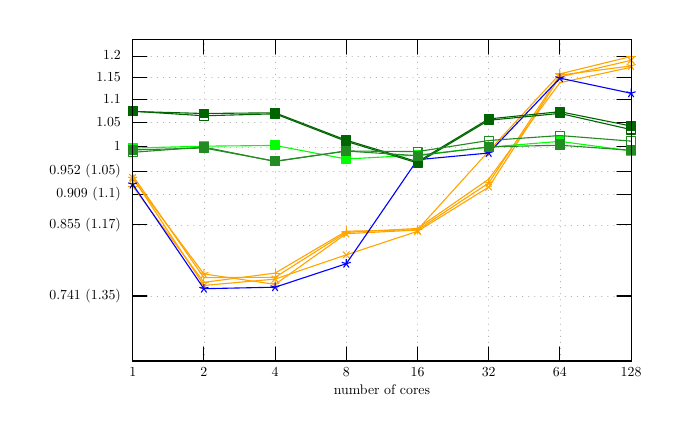
\begin{tikzpicture}[gnuplot]
%% generated with GNUPLOT 6.0p1 (Lua 5.4; terminal rev. Jun 2020, script rev. 118)
%% mar. 14 janv. 2025 16:25:27
\tikzset{every node/.append style={scale=0.50}}
\path (0.000,0.000) rectangle (8.125,4.725);
\gpcolor{color=gp lt color axes}
\gpsetlinetype{gp lt axes}
\gpsetdashtype{gp dt axes}
\gpsetlinewidth{0.50}
\draw[gp path] (1.334,1.317)--(7.664,1.317);
\gpcolor{color=gp lt color border}
\gpsetlinetype{gp lt border}
\gpsetdashtype{gp dt solid}
\gpsetlinewidth{1.00}
\draw[gp path] (1.334,1.317)--(1.514,1.317);
\draw[gp path] (7.664,1.317)--(7.484,1.317);
\node[gp node right] at (1.242,1.317) {0.741 (1.35)};
\gpcolor{color=gp lt color axes}
\gpsetlinetype{gp lt axes}
\gpsetdashtype{gp dt axes}
\gpsetlinewidth{0.50}
\draw[gp path] (1.334,2.221)--(7.664,2.221);
\gpcolor{color=gp lt color border}
\gpsetlinetype{gp lt border}
\gpsetdashtype{gp dt solid}
\gpsetlinewidth{1.00}
\draw[gp path] (1.334,2.221)--(1.514,2.221);
\draw[gp path] (7.664,2.221)--(7.484,2.221);
\node[gp node right] at (1.242,2.221) {0.855 (1.17)};
\gpcolor{color=gp lt color axes}
\gpsetlinetype{gp lt axes}
\gpsetdashtype{gp dt axes}
\gpsetlinewidth{0.50}
\draw[gp path] (1.334,2.610)--(7.664,2.610);
\gpcolor{color=gp lt color border}
\gpsetlinetype{gp lt border}
\gpsetdashtype{gp dt solid}
\gpsetlinewidth{1.00}
\draw[gp path] (1.334,2.610)--(1.514,2.610);
\draw[gp path] (7.664,2.610)--(7.484,2.610);
\node[gp node right] at (1.242,2.610) {0.909 (1.1)};
\gpcolor{color=gp lt color axes}
\gpsetlinetype{gp lt axes}
\gpsetdashtype{gp dt axes}
\gpsetlinewidth{0.50}
\draw[gp path] (1.334,2.904)--(7.664,2.904);
\gpcolor{color=gp lt color border}
\gpsetlinetype{gp lt border}
\gpsetdashtype{gp dt solid}
\gpsetlinewidth{1.00}
\draw[gp path] (1.334,2.904)--(1.514,2.904);
\draw[gp path] (7.664,2.904)--(7.484,2.904);
\node[gp node right] at (1.242,2.904) {0.952 (1.05)};
\gpcolor{color=gp lt color axes}
\gpsetlinetype{gp lt axes}
\gpsetdashtype{gp dt axes}
\gpsetlinewidth{0.50}
\draw[gp path] (1.334,3.212)--(7.664,3.212);
\gpcolor{color=gp lt color border}
\gpsetlinetype{gp lt border}
\gpsetdashtype{gp dt solid}
\gpsetlinewidth{1.00}
\draw[gp path] (1.334,3.212)--(1.514,3.212);
\draw[gp path] (7.664,3.212)--(7.484,3.212);
\node[gp node right] at (1.242,3.212) {$1$};
\gpcolor{color=gp lt color axes}
\gpsetlinetype{gp lt axes}
\gpsetdashtype{gp dt axes}
\gpsetlinewidth{0.50}
\draw[gp path] (1.334,3.520)--(7.664,3.520);
\gpcolor{color=gp lt color border}
\gpsetlinetype{gp lt border}
\gpsetdashtype{gp dt solid}
\gpsetlinewidth{1.00}
\draw[gp path] (1.334,3.520)--(1.514,3.520);
\draw[gp path] (7.664,3.520)--(7.484,3.520);
\node[gp node right] at (1.242,3.520) {$1.05$};
\gpcolor{color=gp lt color axes}
\gpsetlinetype{gp lt axes}
\gpsetdashtype{gp dt axes}
\gpsetlinewidth{0.50}
\draw[gp path] (1.334,3.814)--(7.664,3.814);
\gpcolor{color=gp lt color border}
\gpsetlinetype{gp lt border}
\gpsetdashtype{gp dt solid}
\gpsetlinewidth{1.00}
\draw[gp path] (1.334,3.814)--(1.514,3.814);
\draw[gp path] (7.664,3.814)--(7.484,3.814);
\node[gp node right] at (1.242,3.814) {$1.1$};
\gpcolor{color=gp lt color axes}
\gpsetlinetype{gp lt axes}
\gpsetdashtype{gp dt axes}
\gpsetlinewidth{0.50}
\draw[gp path] (1.334,4.094)--(7.664,4.094);
\gpcolor{color=gp lt color border}
\gpsetlinetype{gp lt border}
\gpsetdashtype{gp dt solid}
\gpsetlinewidth{1.00}
\draw[gp path] (1.334,4.094)--(1.514,4.094);
\draw[gp path] (7.664,4.094)--(7.484,4.094);
\node[gp node right] at (1.242,4.094) {$1.15$};
\gpcolor{color=gp lt color axes}
\gpsetlinetype{gp lt axes}
\gpsetdashtype{gp dt axes}
\gpsetlinewidth{0.50}
\draw[gp path] (1.334,4.363)--(7.664,4.363);
\gpcolor{color=gp lt color border}
\gpsetlinetype{gp lt border}
\gpsetdashtype{gp dt solid}
\gpsetlinewidth{1.00}
\draw[gp path] (1.334,4.363)--(1.514,4.363);
\draw[gp path] (7.664,4.363)--(7.484,4.363);
\node[gp node right] at (1.242,4.363) {$1.2$};
\gpcolor{color=gp lt color axes}
\gpsetlinetype{gp lt axes}
\gpsetdashtype{gp dt axes}
\gpsetlinewidth{0.50}
\draw[gp path] (1.334,0.492)--(1.334,4.570);
\gpcolor{color=gp lt color border}
\gpsetlinetype{gp lt border}
\gpsetdashtype{gp dt solid}
\gpsetlinewidth{1.00}
\draw[gp path] (1.334,0.492)--(1.334,0.672);
\draw[gp path] (1.334,4.570)--(1.334,4.390);
\node[gp node center] at (1.334,0.338) {1};
\gpcolor{color=gp lt color axes}
\gpsetlinetype{gp lt axes}
\gpsetdashtype{gp dt axes}
\gpsetlinewidth{0.50}
\draw[gp path] (2.238,0.492)--(2.238,4.570);
\gpcolor{color=gp lt color border}
\gpsetlinetype{gp lt border}
\gpsetdashtype{gp dt solid}
\gpsetlinewidth{1.00}
\draw[gp path] (2.238,0.492)--(2.238,0.672);
\draw[gp path] (2.238,4.570)--(2.238,4.390);
\node[gp node center] at (2.238,0.338) {2};
\gpcolor{color=gp lt color axes}
\gpsetlinetype{gp lt axes}
\gpsetdashtype{gp dt axes}
\gpsetlinewidth{0.50}
\draw[gp path] (3.142,0.492)--(3.142,4.570);
\gpcolor{color=gp lt color border}
\gpsetlinetype{gp lt border}
\gpsetdashtype{gp dt solid}
\gpsetlinewidth{1.00}
\draw[gp path] (3.142,0.492)--(3.142,0.672);
\draw[gp path] (3.142,4.570)--(3.142,4.390);
\node[gp node center] at (3.142,0.338) {4};
\gpcolor{color=gp lt color axes}
\gpsetlinetype{gp lt axes}
\gpsetdashtype{gp dt axes}
\gpsetlinewidth{0.50}
\draw[gp path] (4.046,0.492)--(4.046,4.570);
\gpcolor{color=gp lt color border}
\gpsetlinetype{gp lt border}
\gpsetdashtype{gp dt solid}
\gpsetlinewidth{1.00}
\draw[gp path] (4.046,0.492)--(4.046,0.672);
\draw[gp path] (4.046,4.570)--(4.046,4.390);
\node[gp node center] at (4.046,0.338) {8};
\gpcolor{color=gp lt color axes}
\gpsetlinetype{gp lt axes}
\gpsetdashtype{gp dt axes}
\gpsetlinewidth{0.50}
\draw[gp path] (4.951,0.492)--(4.951,4.570);
\gpcolor{color=gp lt color border}
\gpsetlinetype{gp lt border}
\gpsetdashtype{gp dt solid}
\gpsetlinewidth{1.00}
\draw[gp path] (4.951,0.492)--(4.951,0.672);
\draw[gp path] (4.951,4.570)--(4.951,4.390);
\node[gp node center] at (4.951,0.338) {16};
\gpcolor{color=gp lt color axes}
\gpsetlinetype{gp lt axes}
\gpsetdashtype{gp dt axes}
\gpsetlinewidth{0.50}
\draw[gp path] (5.855,0.492)--(5.855,4.570);
\gpcolor{color=gp lt color border}
\gpsetlinetype{gp lt border}
\gpsetdashtype{gp dt solid}
\gpsetlinewidth{1.00}
\draw[gp path] (5.855,0.492)--(5.855,0.672);
\draw[gp path] (5.855,4.570)--(5.855,4.390);
\node[gp node center] at (5.855,0.338) {32};
\gpcolor{color=gp lt color axes}
\gpsetlinetype{gp lt axes}
\gpsetdashtype{gp dt axes}
\gpsetlinewidth{0.50}
\draw[gp path] (6.759,0.492)--(6.759,4.570);
\gpcolor{color=gp lt color border}
\gpsetlinetype{gp lt border}
\gpsetdashtype{gp dt solid}
\gpsetlinewidth{1.00}
\draw[gp path] (6.759,0.492)--(6.759,0.672);
\draw[gp path] (6.759,4.570)--(6.759,4.390);
\node[gp node center] at (6.759,0.338) {64};
\gpcolor{color=gp lt color axes}
\gpsetlinetype{gp lt axes}
\gpsetdashtype{gp dt axes}
\gpsetlinewidth{0.50}
\draw[gp path] (7.663,0.492)--(7.663,4.570);
\gpcolor{color=gp lt color border}
\gpsetlinetype{gp lt border}
\gpsetdashtype{gp dt solid}
\gpsetlinewidth{1.00}
\draw[gp path] (7.663,0.492)--(7.663,0.672);
\draw[gp path] (7.663,4.570)--(7.663,4.390);
\node[gp node center] at (7.663,0.338) {128};
\draw[gp path] (1.334,4.570)--(1.334,0.492)--(7.664,0.492)--(7.664,4.570)--cycle;
\gpcolor{rgb color={1.000,0.647,0.000}}
\draw[gp path] (1.334,2.711)--(2.238,1.491)--(3.142,1.608)--(4.046,2.140)--(4.951,2.159)%
  --(5.855,3.157)--(6.759,4.138)--(7.663,4.359);
\gpsetpointsize{4.00}
\gp3point{gp mark 1}{}{(1.334,2.711)}
\gp3point{gp mark 1}{}{(2.238,1.491)}
\gp3point{gp mark 1}{}{(3.142,1.608)}
\gp3point{gp mark 1}{}{(4.046,2.140)}
\gp3point{gp mark 1}{}{(4.951,2.159)}
\gp3point{gp mark 1}{}{(5.855,3.157)}
\gp3point{gp mark 1}{}{(6.759,4.138)}
\gp3point{gp mark 1}{}{(7.663,4.359)}
\draw[gp path] (1.334,2.822)--(2.238,1.451)--(3.142,1.532)--(4.046,1.840)--(4.951,2.139)%
  --(5.855,2.700)--(6.759,4.099)--(7.663,4.310);
\gp3point{gp mark 2}{}{(1.334,2.822)}
\gp3point{gp mark 2}{}{(2.238,1.451)}
\gp3point{gp mark 2}{}{(3.142,1.532)}
\gp3point{gp mark 2}{}{(4.046,1.840)}
\gp3point{gp mark 2}{}{(4.951,2.139)}
\gp3point{gp mark 2}{}{(5.855,2.700)}
\gp3point{gp mark 2}{}{(6.759,4.099)}
\gp3point{gp mark 2}{}{(7.663,4.310)}
\draw[gp path] (1.334,2.808)--(2.238,1.597)--(3.142,1.465)--(4.046,2.109)--(4.951,2.155)%
  --(5.855,2.752)--(6.759,4.122)--(7.663,4.239);
\gp3point{gp mark 3}{}{(1.334,2.808)}
\gp3point{gp mark 3}{}{(2.238,1.597)}
\gp3point{gp mark 3}{}{(3.142,1.465)}
\gp3point{gp mark 3}{}{(4.046,2.109)}
\gp3point{gp mark 3}{}{(4.951,2.155)}
\gp3point{gp mark 3}{}{(5.855,2.752)}
\gp3point{gp mark 3}{}{(6.759,4.122)}
\gp3point{gp mark 3}{}{(7.663,4.239)}
\draw[gp path] (1.334,2.847)--(2.238,1.550)--(3.142,1.555)--(4.046,2.125)--(4.951,2.175)%
  --(5.855,2.801)--(6.759,4.026)--(7.663,4.222);
\gp3point{gp mark 0}{}{(1.334,2.847)}
\gp3point{gp mark 0}{}{(2.238,1.550)}
\gp3point{gp mark 0}{}{(3.142,1.555)}
\gp3point{gp mark 0}{}{(4.046,2.125)}
\gp3point{gp mark 0}{}{(4.951,2.175)}
\gp3point{gp mark 0}{}{(5.855,2.801)}
\gp3point{gp mark 0}{}{(6.759,4.026)}
\gp3point{gp mark 0}{}{(7.663,4.222)}
\gpcolor{rgb color={0.000,0.000,1.000}}
\draw[gp path] (1.334,2.735)--(2.238,1.410)--(3.142,1.429)--(4.046,1.727)--(4.951,3.048)%
  --(5.855,3.133)--(6.759,4.084)--(7.663,3.892);
\gp3point{gp mark 3}{}{(1.334,2.735)}
\gp3point{gp mark 3}{}{(2.238,1.410)}
\gp3point{gp mark 3}{}{(3.142,1.429)}
\gp3point{gp mark 3}{}{(4.046,1.727)}
\gp3point{gp mark 3}{}{(4.951,3.048)}
\gp3point{gp mark 3}{}{(5.855,3.133)}
\gp3point{gp mark 3}{}{(6.759,4.084)}
\gp3point{gp mark 3}{}{(7.663,3.892)}
\gpcolor{rgb color={0.000,1.000,0.000}}
\draw[gp path] (1.334,3.196)--(2.238,3.220)--(3.142,3.229)--(4.046,3.057)--(4.951,3.107)%
  --(5.855,3.208)--(6.759,3.281)--(7.663,3.160);
\gp3point{gp mark 5}{}{(1.334,3.196)}
\gp3point{gp mark 5}{}{(2.238,3.220)}
\gp3point{gp mark 5}{}{(3.142,3.229)}
\gp3point{gp mark 5}{}{(4.046,3.057)}
\gp3point{gp mark 5}{}{(4.951,3.107)}
\gp3point{gp mark 5}{}{(5.855,3.208)}
\gp3point{gp mark 5}{}{(6.759,3.281)}
\gp3point{gp mark 5}{}{(7.663,3.160)}
\gpcolor{rgb color={0.000,0.392,0.000}}
\draw[gp path] (1.334,3.664)--(2.238,3.606)--(3.142,3.631)--(4.046,3.281)--(4.951,3.007)%
  --(5.855,3.549)--(6.759,3.636)--(7.663,3.431);
\gp3point{gp mark 4}{}{(1.334,3.664)}
\gp3point{gp mark 4}{}{(2.238,3.606)}
\gp3point{gp mark 4}{}{(3.142,3.631)}
\gp3point{gp mark 4}{}{(4.046,3.281)}
\gp3point{gp mark 4}{}{(4.951,3.007)}
\gp3point{gp mark 4}{}{(5.855,3.549)}
\gp3point{gp mark 4}{}{(6.759,3.636)}
\gp3point{gp mark 4}{}{(7.663,3.431)}
\draw[gp path] (1.334,3.661)--(2.238,3.635)--(3.142,3.644)--(4.046,3.296)--(4.951,3.022)%
  --(5.855,3.566)--(6.759,3.658)--(7.663,3.476);
\gp3point{gp mark 5}{}{(1.334,3.661)}
\gp3point{gp mark 5}{}{(2.238,3.635)}
\gp3point{gp mark 5}{}{(3.142,3.644)}
\gp3point{gp mark 5}{}{(4.046,3.296)}
\gp3point{gp mark 5}{}{(4.951,3.022)}
\gp3point{gp mark 5}{}{(5.855,3.566)}
\gp3point{gp mark 5}{}{(6.759,3.658)}
\gp3point{gp mark 5}{}{(7.663,3.476)}
\gpcolor{rgb color={0.133,0.545,0.133}}
\draw[gp path] (1.334,3.142)--(2.238,3.209)--(3.142,3.026)--(4.046,3.159)--(4.951,3.151)%
  --(5.855,3.292)--(6.759,3.355)--(7.663,3.284);
\gp3point{gp mark 4}{}{(1.334,3.142)}
\gp3point{gp mark 4}{}{(2.238,3.209)}
\gp3point{gp mark 4}{}{(3.142,3.026)}
\gp3point{gp mark 4}{}{(4.046,3.159)}
\gp3point{gp mark 4}{}{(4.951,3.151)}
\gp3point{gp mark 4}{}{(5.855,3.292)}
\gp3point{gp mark 4}{}{(6.759,3.355)}
\gp3point{gp mark 4}{}{(7.663,3.284)}
\draw[gp path] (1.334,3.172)--(2.238,3.197)--(3.142,3.029)--(4.046,3.158)--(4.951,3.099)%
  --(5.855,3.211)--(6.759,3.232)--(7.663,3.168);
\gp3point{gp mark 5}{}{(1.334,3.172)}
\gp3point{gp mark 5}{}{(2.238,3.197)}
\gp3point{gp mark 5}{}{(3.142,3.029)}
\gp3point{gp mark 5}{}{(4.046,3.158)}
\gp3point{gp mark 5}{}{(4.951,3.099)}
\gp3point{gp mark 5}{}{(5.855,3.211)}
\gp3point{gp mark 5}{}{(6.759,3.232)}
\gp3point{gp mark 5}{}{(7.663,3.168)}
\gpcolor{color=gp lt color border}
\draw[gp path] (1.334,4.570)--(1.334,0.492)--(7.664,0.492)--(7.664,4.570)--cycle;
\node[gp node center] at (4.499,0.107) {number of cores};
%% coordinates of the plot area
\gpdefrectangularnode{gp plot 1}{\pgfpoint{1.334cm}{0.492cm}}{\pgfpoint{7.664cm}{4.570cm}}
\end{tikzpicture}
%% gnuplot variables
\label{time_nl_r}}\\
	\subfloat[Outputs (in s)]{
		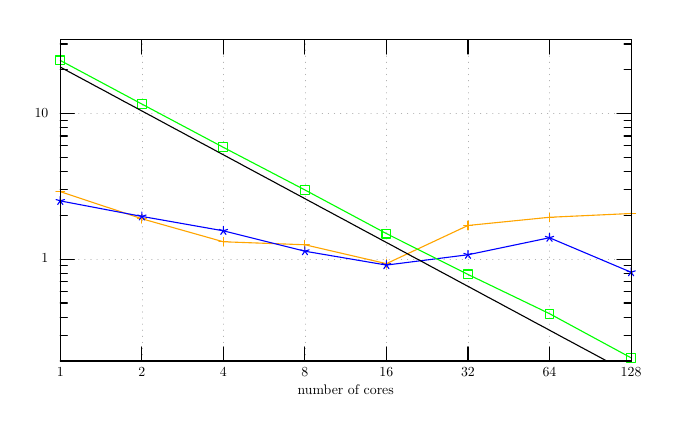
\begin{tikzpicture}[gnuplot]
%% generated with GNUPLOT 6.0p1 (Lua 5.4; terminal rev. Jun 2020, script rev. 118)
%% ven. 10 janv. 2025 17:58:53
\tikzset{every node/.append style={scale=0.50}}
\path (0.000,0.000) rectangle (8.125,4.725);
\gpcolor{color=gp lt color border}
\gpsetlinetype{gp lt border}
\gpsetdashtype{gp dt solid}
\gpsetlinewidth{1.00}
\draw[gp path] (0.414,0.492)--(0.504,0.492);
\draw[gp path] (7.664,0.492)--(7.574,0.492);
\draw[gp path] (0.414,0.818)--(0.504,0.818);
\draw[gp path] (7.664,0.818)--(7.574,0.818);
\draw[gp path] (0.414,1.049)--(0.504,1.049);
\draw[gp path] (7.664,1.049)--(7.574,1.049);
\draw[gp path] (0.414,1.228)--(0.504,1.228);
\draw[gp path] (7.664,1.228)--(7.574,1.228);
\draw[gp path] (0.414,1.375)--(0.504,1.375);
\draw[gp path] (7.664,1.375)--(7.574,1.375);
\draw[gp path] (0.414,1.499)--(0.504,1.499);
\draw[gp path] (7.664,1.499)--(7.574,1.499);
\draw[gp path] (0.414,1.606)--(0.504,1.606);
\draw[gp path] (7.664,1.606)--(7.574,1.606);
\draw[gp path] (0.414,1.701)--(0.504,1.701);
\draw[gp path] (7.664,1.701)--(7.574,1.701);
\gpcolor{color=gp lt color axes}
\gpsetlinetype{gp lt axes}
\gpsetdashtype{gp dt axes}
\gpsetlinewidth{0.50}
\draw[gp path] (0.414,1.785)--(7.664,1.785);
\gpcolor{color=gp lt color border}
\gpsetlinetype{gp lt border}
\gpsetdashtype{gp dt solid}
\gpsetlinewidth{1.00}
\draw[gp path] (0.414,1.785)--(0.594,1.785);
\draw[gp path] (7.664,1.785)--(7.484,1.785);
\node[gp node right] at (0.322,1.785) {$1$};
\draw[gp path] (0.414,2.342)--(0.504,2.342);
\draw[gp path] (7.664,2.342)--(7.574,2.342);
\draw[gp path] (0.414,2.668)--(0.504,2.668);
\draw[gp path] (7.664,2.668)--(7.574,2.668);
\draw[gp path] (0.414,2.899)--(0.504,2.899);
\draw[gp path] (7.664,2.899)--(7.574,2.899);
\draw[gp path] (0.414,3.078)--(0.504,3.078);
\draw[gp path] (7.664,3.078)--(7.574,3.078);
\draw[gp path] (0.414,3.225)--(0.504,3.225);
\draw[gp path] (7.664,3.225)--(7.574,3.225);
\draw[gp path] (0.414,3.349)--(0.504,3.349);
\draw[gp path] (7.664,3.349)--(7.574,3.349);
\draw[gp path] (0.414,3.456)--(0.504,3.456);
\draw[gp path] (7.664,3.456)--(7.574,3.456);
\draw[gp path] (0.414,3.551)--(0.504,3.551);
\draw[gp path] (7.664,3.551)--(7.574,3.551);
\gpcolor{color=gp lt color axes}
\gpsetlinetype{gp lt axes}
\gpsetdashtype{gp dt axes}
\gpsetlinewidth{0.50}
\draw[gp path] (0.414,3.635)--(7.664,3.635);
\gpcolor{color=gp lt color border}
\gpsetlinetype{gp lt border}
\gpsetdashtype{gp dt solid}
\gpsetlinewidth{1.00}
\draw[gp path] (0.414,3.635)--(0.594,3.635);
\draw[gp path] (7.664,3.635)--(7.484,3.635);
\node[gp node right] at (0.322,3.635) {$10$};
\draw[gp path] (0.414,4.192)--(0.504,4.192);
\draw[gp path] (7.664,4.192)--(7.574,4.192);
\draw[gp path] (0.414,4.518)--(0.504,4.518);
\draw[gp path] (7.664,4.518)--(7.574,4.518);
\gpcolor{color=gp lt color axes}
\gpsetlinetype{gp lt axes}
\gpsetdashtype{gp dt axes}
\gpsetlinewidth{0.50}
\draw[gp path] (0.414,0.492)--(0.414,4.570);
\gpcolor{color=gp lt color border}
\gpsetlinetype{gp lt border}
\gpsetdashtype{gp dt solid}
\gpsetlinewidth{1.00}
\draw[gp path] (0.414,0.492)--(0.414,0.672);
\draw[gp path] (0.414,4.570)--(0.414,4.390);
\node[gp node center] at (0.414,0.338) {1};
\gpcolor{color=gp lt color axes}
\gpsetlinetype{gp lt axes}
\gpsetdashtype{gp dt axes}
\gpsetlinewidth{0.50}
\draw[gp path] (1.450,0.492)--(1.450,4.570);
\gpcolor{color=gp lt color border}
\gpsetlinetype{gp lt border}
\gpsetdashtype{gp dt solid}
\gpsetlinewidth{1.00}
\draw[gp path] (1.450,0.492)--(1.450,0.672);
\draw[gp path] (1.450,4.570)--(1.450,4.390);
\node[gp node center] at (1.450,0.338) {2};
\gpcolor{color=gp lt color axes}
\gpsetlinetype{gp lt axes}
\gpsetdashtype{gp dt axes}
\gpsetlinewidth{0.50}
\draw[gp path] (2.485,0.492)--(2.485,4.570);
\gpcolor{color=gp lt color border}
\gpsetlinetype{gp lt border}
\gpsetdashtype{gp dt solid}
\gpsetlinewidth{1.00}
\draw[gp path] (2.485,0.492)--(2.485,0.672);
\draw[gp path] (2.485,4.570)--(2.485,4.390);
\node[gp node center] at (2.485,0.338) {4};
\gpcolor{color=gp lt color axes}
\gpsetlinetype{gp lt axes}
\gpsetdashtype{gp dt axes}
\gpsetlinewidth{0.50}
\draw[gp path] (3.521,0.492)--(3.521,4.570);
\gpcolor{color=gp lt color border}
\gpsetlinetype{gp lt border}
\gpsetdashtype{gp dt solid}
\gpsetlinewidth{1.00}
\draw[gp path] (3.521,0.492)--(3.521,0.672);
\draw[gp path] (3.521,4.570)--(3.521,4.390);
\node[gp node center] at (3.521,0.338) {8};
\gpcolor{color=gp lt color axes}
\gpsetlinetype{gp lt axes}
\gpsetdashtype{gp dt axes}
\gpsetlinewidth{0.50}
\draw[gp path] (4.556,0.492)--(4.556,4.570);
\gpcolor{color=gp lt color border}
\gpsetlinetype{gp lt border}
\gpsetdashtype{gp dt solid}
\gpsetlinewidth{1.00}
\draw[gp path] (4.556,0.492)--(4.556,0.672);
\draw[gp path] (4.556,4.570)--(4.556,4.390);
\node[gp node center] at (4.556,0.338) {16};
\gpcolor{color=gp lt color axes}
\gpsetlinetype{gp lt axes}
\gpsetdashtype{gp dt axes}
\gpsetlinewidth{0.50}
\draw[gp path] (5.592,0.492)--(5.592,4.570);
\gpcolor{color=gp lt color border}
\gpsetlinetype{gp lt border}
\gpsetdashtype{gp dt solid}
\gpsetlinewidth{1.00}
\draw[gp path] (5.592,0.492)--(5.592,0.672);
\draw[gp path] (5.592,4.570)--(5.592,4.390);
\node[gp node center] at (5.592,0.338) {32};
\gpcolor{color=gp lt color axes}
\gpsetlinetype{gp lt axes}
\gpsetdashtype{gp dt axes}
\gpsetlinewidth{0.50}
\draw[gp path] (6.627,0.492)--(6.627,4.570);
\gpcolor{color=gp lt color border}
\gpsetlinetype{gp lt border}
\gpsetdashtype{gp dt solid}
\gpsetlinewidth{1.00}
\draw[gp path] (6.627,0.492)--(6.627,0.672);
\draw[gp path] (6.627,4.570)--(6.627,4.390);
\node[gp node center] at (6.627,0.338) {64};
\gpcolor{color=gp lt color axes}
\gpsetlinetype{gp lt axes}
\gpsetdashtype{gp dt axes}
\gpsetlinewidth{0.50}
\draw[gp path] (7.663,0.492)--(7.663,4.570);
\gpcolor{color=gp lt color border}
\gpsetlinetype{gp lt border}
\gpsetdashtype{gp dt solid}
\gpsetlinewidth{1.00}
\draw[gp path] (7.663,0.492)--(7.663,0.672);
\draw[gp path] (7.663,4.570)--(7.663,4.390);
\node[gp node center] at (7.663,0.338) {128};
\draw[gp path] (0.414,4.570)--(0.414,0.492)--(7.664,0.492)--(7.664,4.570)--cycle;
\gpcolor{rgb color={1.000,0.647,0.000}}
\draw[gp path] (0.414,2.643)--(1.450,2.298)--(2.485,2.006)--(3.521,1.968)--(4.556,1.728)%
  --(5.592,2.213)--(6.627,2.317)--(7.663,2.365);
\gpsetpointsize{4.00}
\gp3point{gp mark 1}{}{(0.414,2.643)}
\gp3point{gp mark 1}{}{(1.450,2.298)}
\gp3point{gp mark 1}{}{(2.485,2.006)}
\gp3point{gp mark 1}{}{(3.521,1.968)}
\gp3point{gp mark 1}{}{(4.556,1.728)}
\gp3point{gp mark 1}{}{(5.592,2.213)}
\gp3point{gp mark 1}{}{(6.627,2.317)}
\gp3point{gp mark 1}{}{(7.663,2.365)}
\gpcolor{rgb color={0.000,0.000,1.000}}
\draw[gp path] (0.414,2.525)--(1.450,2.328)--(2.485,2.145)--(3.521,1.886)--(4.556,1.710)%
  --(5.592,1.841)--(6.627,2.057)--(7.663,1.619);
\gp3point{gp mark 3}{}{(0.414,2.525)}
\gp3point{gp mark 3}{}{(1.450,2.328)}
\gp3point{gp mark 3}{}{(2.485,2.145)}
\gp3point{gp mark 3}{}{(3.521,1.886)}
\gp3point{gp mark 3}{}{(4.556,1.710)}
\gp3point{gp mark 3}{}{(5.592,1.841)}
\gp3point{gp mark 3}{}{(6.627,2.057)}
\gp3point{gp mark 3}{}{(7.663,1.619)}
\gpcolor{rgb color={0.000,1.000,0.000}}
\draw[gp path] (0.414,4.309)--(1.450,3.755)--(2.485,3.205)--(3.521,2.664)--(4.556,2.110)%
  --(5.592,1.591)--(6.627,1.093)--(7.663,0.532);
\gp3point{gp mark 4}{}{(0.414,4.309)}
\gp3point{gp mark 4}{}{(1.450,3.755)}
\gp3point{gp mark 4}{}{(2.485,3.205)}
\gp3point{gp mark 4}{}{(3.521,2.664)}
\gp3point{gp mark 4}{}{(4.556,2.110)}
\gp3point{gp mark 4}{}{(5.592,1.591)}
\gp3point{gp mark 4}{}{(6.627,1.093)}
\gp3point{gp mark 4}{}{(7.663,0.532)}
\gpcolor{rgb color={0.000,0.000,0.000}}
\draw[gp path] (0.414,4.225)--(0.487,4.185)--(0.560,4.146)--(0.634,4.106)--(0.707,4.067)%
  --(0.780,4.028)--(0.853,3.988)--(0.927,3.949)--(1.000,3.910)--(1.073,3.870)--(1.146,3.831)%
  --(1.219,3.791)--(1.293,3.752)--(1.366,3.713)--(1.439,3.673)--(1.512,3.634)--(1.586,3.595)%
  --(1.659,3.555)--(1.732,3.516)--(1.805,3.476)--(1.878,3.437)--(1.952,3.398)--(2.025,3.358)%
  --(2.098,3.319)--(2.171,3.279)--(2.245,3.240)--(2.318,3.201)--(2.391,3.161)--(2.464,3.122)%
  --(2.537,3.083)--(2.611,3.043)--(2.684,3.004)--(2.757,2.964)--(2.830,2.925)--(2.903,2.886)%
  --(2.977,2.846)--(3.050,2.807)--(3.123,2.768)--(3.196,2.728)--(3.270,2.689)--(3.343,2.649)%
  --(3.416,2.610)--(3.489,2.571)--(3.562,2.531)--(3.636,2.492)--(3.709,2.452)--(3.782,2.413)%
  --(3.855,2.374)--(3.929,2.334)--(4.002,2.295)--(4.075,2.256)--(4.148,2.216)--(4.221,2.177)%
  --(4.295,2.137)--(4.368,2.098)--(4.441,2.059)--(4.514,2.019)--(4.588,1.980)--(4.661,1.941)%
  --(4.734,1.901)--(4.807,1.862)--(4.880,1.822)--(4.954,1.783)--(5.027,1.744)--(5.100,1.704)%
  --(5.173,1.665)--(5.247,1.625)--(5.320,1.586)--(5.393,1.547)--(5.466,1.507)--(5.539,1.468)%
  --(5.613,1.429)--(5.686,1.389)--(5.759,1.350)--(5.832,1.310)--(5.906,1.271)--(5.979,1.232)%
  --(6.052,1.192)--(6.125,1.153)--(6.198,1.114)--(6.272,1.074)--(6.345,1.035)--(6.418,0.995)%
  --(6.491,0.956)--(6.565,0.917)--(6.638,0.877)--(6.711,0.838)--(6.784,0.798)--(6.857,0.759)%
  --(6.931,0.720)--(7.004,0.680)--(7.077,0.641)--(7.150,0.602)--(7.224,0.562)--(7.297,0.523)%
  --(7.353,0.492);
\gpcolor{color=gp lt color border}
\draw[gp path] (0.414,4.570)--(0.414,0.492)--(7.664,0.492)--(7.664,4.570)--cycle;
\node[gp node center] at (4.039,0.107) {number of cores};
%% coordinates of the plot area
\gpdefrectangularnode{gp plot 1}{\pgfpoint{0.414cm}{0.492cm}}{\pgfpoint{7.664cm}{4.570cm}}
\end{tikzpicture}
%% gnuplot variables
\label{time_output}
	}
	\subfloat[Outputs (Ratio vs MFEM)]{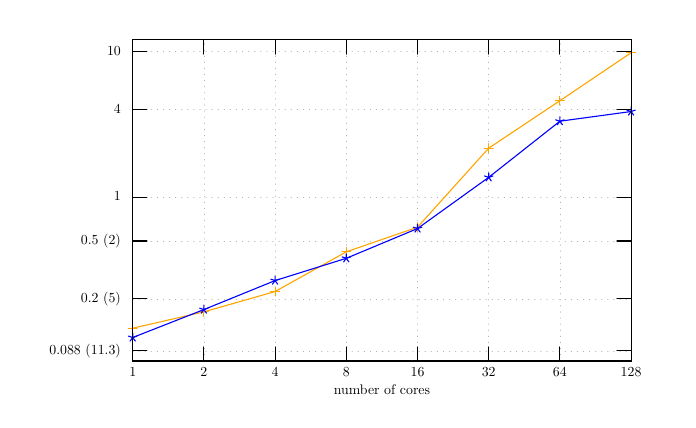
\begin{tikzpicture}[gnuplot]
%% generated with GNUPLOT 6.0p1 (Lua 5.4; terminal rev. Jun 2020, script rev. 118)
%% ven. 10 janv. 2025 17:58:53
\tikzset{every node/.append style={scale=0.50}}
\path (0.000,0.000) rectangle (8.125,4.725);
\gpcolor{color=gp lt color axes}
\gpsetlinetype{gp lt axes}
\gpsetdashtype{gp dt axes}
\gpsetlinewidth{0.50}
\draw[gp path] (1.334,0.620)--(7.664,0.620);
\gpcolor{color=gp lt color border}
\gpsetlinetype{gp lt border}
\gpsetdashtype{gp dt solid}
\gpsetlinewidth{1.00}
\draw[gp path] (1.334,0.620)--(1.514,0.620);
\draw[gp path] (7.664,0.620)--(7.484,0.620);
\node[gp node right] at (1.242,0.620) {0.088 (11.3)};
\gpcolor{color=gp lt color axes}
\gpsetlinetype{gp lt axes}
\gpsetdashtype{gp dt axes}
\gpsetlinewidth{0.50}
\draw[gp path] (1.334,1.280)--(7.664,1.280);
\gpcolor{color=gp lt color border}
\gpsetlinetype{gp lt border}
\gpsetdashtype{gp dt solid}
\gpsetlinewidth{1.00}
\draw[gp path] (1.334,1.280)--(1.514,1.280);
\draw[gp path] (7.664,1.280)--(7.484,1.280);
\node[gp node right] at (1.242,1.280) {0.2 (5)};
\gpcolor{color=gp lt color axes}
\gpsetlinetype{gp lt axes}
\gpsetdashtype{gp dt axes}
\gpsetlinewidth{0.50}
\draw[gp path] (1.334,2.016)--(7.664,2.016);
\gpcolor{color=gp lt color border}
\gpsetlinetype{gp lt border}
\gpsetdashtype{gp dt solid}
\gpsetlinewidth{1.00}
\draw[gp path] (1.334,2.016)--(1.514,2.016);
\draw[gp path] (7.664,2.016)--(7.484,2.016);
\node[gp node right] at (1.242,2.016) {0.5 (2)};
\gpcolor{color=gp lt color axes}
\gpsetlinetype{gp lt axes}
\gpsetdashtype{gp dt axes}
\gpsetlinewidth{0.50}
\draw[gp path] (1.334,2.573)--(7.664,2.573);
\gpcolor{color=gp lt color border}
\gpsetlinetype{gp lt border}
\gpsetdashtype{gp dt solid}
\gpsetlinewidth{1.00}
\draw[gp path] (1.334,2.573)--(1.514,2.573);
\draw[gp path] (7.664,2.573)--(7.484,2.573);
\node[gp node right] at (1.242,2.573) {$1$};
\gpcolor{color=gp lt color axes}
\gpsetlinetype{gp lt axes}
\gpsetdashtype{gp dt axes}
\gpsetlinewidth{0.50}
\draw[gp path] (1.334,3.687)--(7.664,3.687);
\gpcolor{color=gp lt color border}
\gpsetlinetype{gp lt border}
\gpsetdashtype{gp dt solid}
\gpsetlinewidth{1.00}
\draw[gp path] (1.334,3.687)--(1.514,3.687);
\draw[gp path] (7.664,3.687)--(7.484,3.687);
\node[gp node right] at (1.242,3.687) {$4$};
\gpcolor{color=gp lt color axes}
\gpsetlinetype{gp lt axes}
\gpsetdashtype{gp dt axes}
\gpsetlinewidth{0.50}
\draw[gp path] (1.334,4.424)--(7.664,4.424);
\gpcolor{color=gp lt color border}
\gpsetlinetype{gp lt border}
\gpsetdashtype{gp dt solid}
\gpsetlinewidth{1.00}
\draw[gp path] (1.334,4.424)--(1.514,4.424);
\draw[gp path] (7.664,4.424)--(7.484,4.424);
\node[gp node right] at (1.242,4.424) {$10$};
\gpcolor{color=gp lt color axes}
\gpsetlinetype{gp lt axes}
\gpsetdashtype{gp dt axes}
\gpsetlinewidth{0.50}
\draw[gp path] (1.334,0.492)--(1.334,4.570);
\gpcolor{color=gp lt color border}
\gpsetlinetype{gp lt border}
\gpsetdashtype{gp dt solid}
\gpsetlinewidth{1.00}
\draw[gp path] (1.334,0.492)--(1.334,0.672);
\draw[gp path] (1.334,4.570)--(1.334,4.390);
\node[gp node center] at (1.334,0.338) {1};
\gpcolor{color=gp lt color axes}
\gpsetlinetype{gp lt axes}
\gpsetdashtype{gp dt axes}
\gpsetlinewidth{0.50}
\draw[gp path] (2.238,0.492)--(2.238,4.570);
\gpcolor{color=gp lt color border}
\gpsetlinetype{gp lt border}
\gpsetdashtype{gp dt solid}
\gpsetlinewidth{1.00}
\draw[gp path] (2.238,0.492)--(2.238,0.672);
\draw[gp path] (2.238,4.570)--(2.238,4.390);
\node[gp node center] at (2.238,0.338) {2};
\gpcolor{color=gp lt color axes}
\gpsetlinetype{gp lt axes}
\gpsetdashtype{gp dt axes}
\gpsetlinewidth{0.50}
\draw[gp path] (3.142,0.492)--(3.142,4.570);
\gpcolor{color=gp lt color border}
\gpsetlinetype{gp lt border}
\gpsetdashtype{gp dt solid}
\gpsetlinewidth{1.00}
\draw[gp path] (3.142,0.492)--(3.142,0.672);
\draw[gp path] (3.142,4.570)--(3.142,4.390);
\node[gp node center] at (3.142,0.338) {4};
\gpcolor{color=gp lt color axes}
\gpsetlinetype{gp lt axes}
\gpsetdashtype{gp dt axes}
\gpsetlinewidth{0.50}
\draw[gp path] (4.046,0.492)--(4.046,4.570);
\gpcolor{color=gp lt color border}
\gpsetlinetype{gp lt border}
\gpsetdashtype{gp dt solid}
\gpsetlinewidth{1.00}
\draw[gp path] (4.046,0.492)--(4.046,0.672);
\draw[gp path] (4.046,4.570)--(4.046,4.390);
\node[gp node center] at (4.046,0.338) {8};
\gpcolor{color=gp lt color axes}
\gpsetlinetype{gp lt axes}
\gpsetdashtype{gp dt axes}
\gpsetlinewidth{0.50}
\draw[gp path] (4.951,0.492)--(4.951,4.570);
\gpcolor{color=gp lt color border}
\gpsetlinetype{gp lt border}
\gpsetdashtype{gp dt solid}
\gpsetlinewidth{1.00}
\draw[gp path] (4.951,0.492)--(4.951,0.672);
\draw[gp path] (4.951,4.570)--(4.951,4.390);
\node[gp node center] at (4.951,0.338) {16};
\gpcolor{color=gp lt color axes}
\gpsetlinetype{gp lt axes}
\gpsetdashtype{gp dt axes}
\gpsetlinewidth{0.50}
\draw[gp path] (5.855,0.492)--(5.855,4.570);
\gpcolor{color=gp lt color border}
\gpsetlinetype{gp lt border}
\gpsetdashtype{gp dt solid}
\gpsetlinewidth{1.00}
\draw[gp path] (5.855,0.492)--(5.855,0.672);
\draw[gp path] (5.855,4.570)--(5.855,4.390);
\node[gp node center] at (5.855,0.338) {32};
\gpcolor{color=gp lt color axes}
\gpsetlinetype{gp lt axes}
\gpsetdashtype{gp dt axes}
\gpsetlinewidth{0.50}
\draw[gp path] (6.759,0.492)--(6.759,4.570);
\gpcolor{color=gp lt color border}
\gpsetlinetype{gp lt border}
\gpsetdashtype{gp dt solid}
\gpsetlinewidth{1.00}
\draw[gp path] (6.759,0.492)--(6.759,0.672);
\draw[gp path] (6.759,4.570)--(6.759,4.390);
\node[gp node center] at (6.759,0.338) {64};
\gpcolor{color=gp lt color axes}
\gpsetlinetype{gp lt axes}
\gpsetdashtype{gp dt axes}
\gpsetlinewidth{0.50}
\draw[gp path] (7.663,0.492)--(7.663,4.570);
\gpcolor{color=gp lt color border}
\gpsetlinetype{gp lt border}
\gpsetdashtype{gp dt solid}
\gpsetlinewidth{1.00}
\draw[gp path] (7.663,0.492)--(7.663,0.672);
\draw[gp path] (7.663,4.570)--(7.663,4.390);
\node[gp node center] at (7.663,0.338) {128};
\draw[gp path] (1.334,4.570)--(1.334,0.492)--(7.664,0.492)--(7.664,4.570)--cycle;
\gpcolor{rgb color={1.000,0.647,0.000}}
\draw[gp path] (1.334,0.908)--(2.238,1.116)--(3.142,1.374)--(4.046,1.878)--(4.951,2.191)%
  --(5.855,3.195)--(6.759,3.797)--(7.663,4.406);
\gpsetpointsize{4.00}
\gp3point{gp mark 1}{}{(1.334,0.908)}
\gp3point{gp mark 1}{}{(2.238,1.116)}
\gp3point{gp mark 1}{}{(3.142,1.374)}
\gp3point{gp mark 1}{}{(4.046,1.878)}
\gp3point{gp mark 1}{}{(4.951,2.191)}
\gp3point{gp mark 1}{}{(5.855,3.195)}
\gp3point{gp mark 1}{}{(6.759,3.797)}
\gp3point{gp mark 1}{}{(7.663,4.406)}
\gpcolor{rgb color={0.000,0.000,1.000}}
\draw[gp path] (1.334,0.790)--(2.238,1.145)--(3.142,1.513)--(4.046,1.796)--(4.951,2.174)%
  --(5.855,2.824)--(6.759,3.537)--(7.663,3.660);
\gp3point{gp mark 3}{}{(1.334,0.790)}
\gp3point{gp mark 3}{}{(2.238,1.145)}
\gp3point{gp mark 3}{}{(3.142,1.513)}
\gp3point{gp mark 3}{}{(4.046,1.796)}
\gp3point{gp mark 3}{}{(4.951,2.174)}
\gp3point{gp mark 3}{}{(5.855,2.824)}
\gp3point{gp mark 3}{}{(6.759,3.537)}
\gp3point{gp mark 3}{}{(7.663,3.660)}
\gpcolor{color=gp lt color border}
\draw[gp path] (1.334,4.570)--(1.334,0.492)--(7.664,0.492)--(7.664,4.570)--cycle;
\node[gp node center] at (4.499,0.107) {number of cores};
%% coordinates of the plot area
\gpdefrectangularnode{gp plot 1}{\pgfpoint{1.334cm}{0.492cm}}{\pgfpoint{7.664cm}{4.570cm}}
\end{tikzpicture}
%% gnuplot variables
\label{time_output_r}}
	\caption{Elapsed time function of the number of processes: Strain/stress creation, non-linear loop and outputs (in log-log scale)\label{elapsed4}}
\end{figure}
\begin{figure}
	\subfloat[Small (in s)]{
		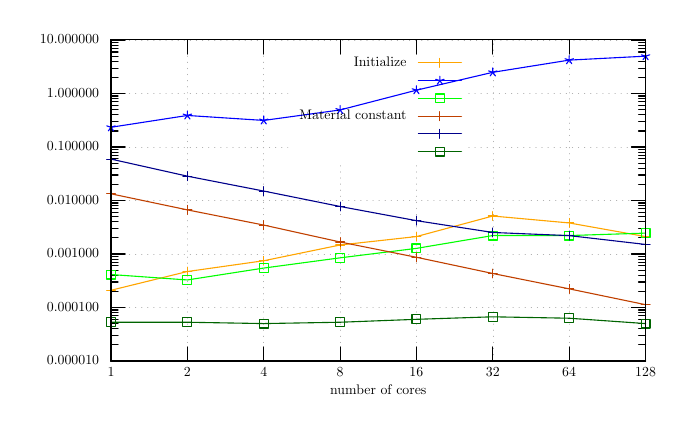
\begin{tikzpicture}[gnuplot]
%% generated with GNUPLOT 6.0p1 (Lua 5.4; terminal rev. Jun 2020, script rev. 118)
%% ven. 10 janv. 2025 17:58:53
\tikzset{every node/.append style={scale=0.50}}
\path (0.000,0.000) rectangle (8.125,4.725);
\gpcolor{color=gp lt color axes}
\gpsetlinetype{gp lt axes}
\gpsetdashtype{gp dt axes}
\gpsetlinewidth{0.50}
\draw[gp path] (1.058,0.492)--(7.848,0.492);
\gpcolor{color=gp lt color border}
\gpsetlinetype{gp lt border}
\gpsetdashtype{gp dt solid}
\gpsetlinewidth{1.00}
\draw[gp path] (1.058,0.492)--(1.238,0.492);
\draw[gp path] (7.848,0.492)--(7.668,0.492);
\node[gp node right] at (0.966,0.492) {0.000010};
\draw[gp path] (1.058,0.696)--(1.148,0.696);
\draw[gp path] (7.848,0.696)--(7.758,0.696);
\draw[gp path] (1.058,0.816)--(1.148,0.816);
\draw[gp path] (7.848,0.816)--(7.758,0.816);
\draw[gp path] (1.058,0.901)--(1.148,0.901);
\draw[gp path] (7.848,0.901)--(7.758,0.901);
\draw[gp path] (1.058,0.967)--(1.148,0.967);
\draw[gp path] (7.848,0.967)--(7.758,0.967);
\draw[gp path] (1.058,1.021)--(1.148,1.021);
\draw[gp path] (7.848,1.021)--(7.758,1.021);
\draw[gp path] (1.058,1.066)--(1.148,1.066);
\draw[gp path] (7.848,1.066)--(7.758,1.066);
\draw[gp path] (1.058,1.105)--(1.148,1.105);
\draw[gp path] (7.848,1.105)--(7.758,1.105);
\draw[gp path] (1.058,1.140)--(1.148,1.140);
\draw[gp path] (7.848,1.140)--(7.758,1.140);
\gpcolor{color=gp lt color axes}
\gpsetlinetype{gp lt axes}
\gpsetdashtype{gp dt axes}
\gpsetlinewidth{0.50}
\draw[gp path] (1.058,1.171)--(7.848,1.171);
\gpcolor{color=gp lt color border}
\gpsetlinetype{gp lt border}
\gpsetdashtype{gp dt solid}
\gpsetlinewidth{1.00}
\draw[gp path] (1.058,1.171)--(1.238,1.171);
\draw[gp path] (7.848,1.171)--(7.668,1.171);
\node[gp node right] at (0.966,1.171) {0.000100};
\draw[gp path] (1.058,1.376)--(1.148,1.376);
\draw[gp path] (7.848,1.376)--(7.758,1.376);
\draw[gp path] (1.058,1.495)--(1.148,1.495);
\draw[gp path] (7.848,1.495)--(7.758,1.495);
\draw[gp path] (1.058,1.580)--(1.148,1.580);
\draw[gp path] (7.848,1.580)--(7.758,1.580);
\draw[gp path] (1.058,1.646)--(1.148,1.646);
\draw[gp path] (7.848,1.646)--(7.758,1.646);
\draw[gp path] (1.058,1.700)--(1.148,1.700);
\draw[gp path] (7.848,1.700)--(7.758,1.700);
\draw[gp path] (1.058,1.745)--(1.148,1.745);
\draw[gp path] (7.848,1.745)--(7.758,1.745);
\draw[gp path] (1.058,1.785)--(1.148,1.785);
\draw[gp path] (7.848,1.785)--(7.758,1.785);
\draw[gp path] (1.058,1.819)--(1.148,1.819);
\draw[gp path] (7.848,1.819)--(7.758,1.819);
\gpcolor{color=gp lt color axes}
\gpsetlinetype{gp lt axes}
\gpsetdashtype{gp dt axes}
\gpsetlinewidth{0.50}
\draw[gp path] (1.058,1.850)--(7.848,1.850);
\gpcolor{color=gp lt color border}
\gpsetlinetype{gp lt border}
\gpsetdashtype{gp dt solid}
\gpsetlinewidth{1.00}
\draw[gp path] (1.058,1.850)--(1.238,1.850);
\draw[gp path] (7.848,1.850)--(7.668,1.850);
\node[gp node right] at (0.966,1.850) {0.001000};
\draw[gp path] (1.058,2.055)--(1.148,2.055);
\draw[gp path] (7.848,2.055)--(7.758,2.055);
\draw[gp path] (1.058,2.174)--(1.148,2.174);
\draw[gp path] (7.848,2.174)--(7.758,2.174);
\draw[gp path] (1.058,2.259)--(1.148,2.259);
\draw[gp path] (7.848,2.259)--(7.758,2.259);
\draw[gp path] (1.058,2.325)--(1.148,2.325);
\draw[gp path] (7.848,2.325)--(7.758,2.325);
\draw[gp path] (1.058,2.379)--(1.148,2.379);
\draw[gp path] (7.848,2.379)--(7.758,2.379);
\draw[gp path] (1.058,2.424)--(1.148,2.424);
\draw[gp path] (7.848,2.424)--(7.758,2.424);
\draw[gp path] (1.058,2.464)--(1.148,2.464);
\draw[gp path] (7.848,2.464)--(7.758,2.464);
\draw[gp path] (1.058,2.498)--(1.148,2.498);
\draw[gp path] (7.848,2.498)--(7.758,2.498);
\gpcolor{color=gp lt color axes}
\gpsetlinetype{gp lt axes}
\gpsetdashtype{gp dt axes}
\gpsetlinewidth{0.50}
\draw[gp path] (1.058,2.530)--(7.848,2.530);
\gpcolor{color=gp lt color border}
\gpsetlinetype{gp lt border}
\gpsetdashtype{gp dt solid}
\gpsetlinewidth{1.00}
\draw[gp path] (1.058,2.530)--(1.238,2.530);
\draw[gp path] (7.848,2.530)--(7.668,2.530);
\node[gp node right] at (0.966,2.530) {0.010000};
\draw[gp path] (1.058,2.734)--(1.148,2.734);
\draw[gp path] (7.848,2.734)--(7.758,2.734);
\draw[gp path] (1.058,2.854)--(1.148,2.854);
\draw[gp path] (7.848,2.854)--(7.758,2.854);
\draw[gp path] (1.058,2.938)--(1.148,2.938);
\draw[gp path] (7.848,2.938)--(7.758,2.938);
\draw[gp path] (1.058,3.004)--(1.148,3.004);
\draw[gp path] (7.848,3.004)--(7.758,3.004);
\draw[gp path] (1.058,3.058)--(1.148,3.058);
\draw[gp path] (7.848,3.058)--(7.758,3.058);
\draw[gp path] (1.058,3.104)--(1.148,3.104);
\draw[gp path] (7.848,3.104)--(7.758,3.104);
\draw[gp path] (1.058,3.143)--(1.148,3.143);
\draw[gp path] (7.848,3.143)--(7.758,3.143);
\draw[gp path] (1.058,3.178)--(1.148,3.178);
\draw[gp path] (7.848,3.178)--(7.758,3.178);
\gpcolor{color=gp lt color axes}
\gpsetlinetype{gp lt axes}
\gpsetdashtype{gp dt axes}
\gpsetlinewidth{0.50}
\draw[gp path] (1.058,3.209)--(3.305,3.209);
\draw[gp path] (5.601,3.209)--(7.848,3.209);
\gpcolor{color=gp lt color border}
\gpsetlinetype{gp lt border}
\gpsetdashtype{gp dt solid}
\gpsetlinewidth{1.00}
\draw[gp path] (1.058,3.209)--(1.238,3.209);
\draw[gp path] (7.848,3.209)--(7.668,3.209);
\node[gp node right] at (0.966,3.209) {0.100000};
\draw[gp path] (1.058,3.413)--(1.148,3.413);
\draw[gp path] (7.848,3.413)--(7.758,3.413);
\draw[gp path] (1.058,3.533)--(1.148,3.533);
\draw[gp path] (7.848,3.533)--(7.758,3.533);
\draw[gp path] (1.058,3.618)--(1.148,3.618);
\draw[gp path] (7.848,3.618)--(7.758,3.618);
\draw[gp path] (1.058,3.683)--(1.148,3.683);
\draw[gp path] (7.848,3.683)--(7.758,3.683);
\draw[gp path] (1.058,3.737)--(1.148,3.737);
\draw[gp path] (7.848,3.737)--(7.758,3.737);
\draw[gp path] (1.058,3.783)--(1.148,3.783);
\draw[gp path] (7.848,3.783)--(7.758,3.783);
\draw[gp path] (1.058,3.822)--(1.148,3.822);
\draw[gp path] (7.848,3.822)--(7.758,3.822);
\draw[gp path] (1.058,3.857)--(1.148,3.857);
\draw[gp path] (7.848,3.857)--(7.758,3.857);
\gpcolor{color=gp lt color axes}
\gpsetlinetype{gp lt axes}
\gpsetdashtype{gp dt axes}
\gpsetlinewidth{0.50}
\draw[gp path] (1.058,3.888)--(3.305,3.888);
\draw[gp path] (5.601,3.888)--(7.848,3.888);
\gpcolor{color=gp lt color border}
\gpsetlinetype{gp lt border}
\gpsetdashtype{gp dt solid}
\gpsetlinewidth{1.00}
\draw[gp path] (1.058,3.888)--(1.238,3.888);
\draw[gp path] (7.848,3.888)--(7.668,3.888);
\node[gp node right] at (0.966,3.888) {1.000000};
\draw[gp path] (1.058,4.092)--(1.148,4.092);
\draw[gp path] (7.848,4.092)--(7.758,4.092);
\draw[gp path] (1.058,4.212)--(1.148,4.212);
\draw[gp path] (7.848,4.212)--(7.758,4.212);
\draw[gp path] (1.058,4.297)--(1.148,4.297);
\draw[gp path] (7.848,4.297)--(7.758,4.297);
\draw[gp path] (1.058,4.363)--(1.148,4.363);
\draw[gp path] (7.848,4.363)--(7.758,4.363);
\draw[gp path] (1.058,4.416)--(1.148,4.416);
\draw[gp path] (7.848,4.416)--(7.758,4.416);
\draw[gp path] (1.058,4.462)--(1.148,4.462);
\draw[gp path] (7.848,4.462)--(7.758,4.462);
\draw[gp path] (1.058,4.501)--(1.148,4.501);
\draw[gp path] (7.848,4.501)--(7.758,4.501);
\draw[gp path] (1.058,4.536)--(1.148,4.536);
\draw[gp path] (7.848,4.536)--(7.758,4.536);
\gpcolor{color=gp lt color axes}
\gpsetlinetype{gp lt axes}
\gpsetdashtype{gp dt axes}
\gpsetlinewidth{0.50}
\draw[gp path] (1.058,4.567)--(7.848,4.567);
\gpcolor{color=gp lt color border}
\gpsetlinetype{gp lt border}
\gpsetdashtype{gp dt solid}
\gpsetlinewidth{1.00}
\draw[gp path] (1.058,4.567)--(1.238,4.567);
\draw[gp path] (7.848,4.567)--(7.668,4.567);
\node[gp node right] at (0.966,4.567) {10.000000};
\gpcolor{color=gp lt color axes}
\gpsetlinetype{gp lt axes}
\gpsetdashtype{gp dt axes}
\gpsetlinewidth{0.50}
\draw[gp path] (1.058,0.492)--(1.058,4.570);
\gpcolor{color=gp lt color border}
\gpsetlinetype{gp lt border}
\gpsetdashtype{gp dt solid}
\gpsetlinewidth{1.00}
\draw[gp path] (1.058,0.492)--(1.058,0.672);
\draw[gp path] (1.058,4.570)--(1.058,4.390);
\node[gp node center] at (1.058,0.338) {1};
\gpcolor{color=gp lt color axes}
\gpsetlinetype{gp lt axes}
\gpsetdashtype{gp dt axes}
\gpsetlinewidth{0.50}
\draw[gp path] (2.028,0.492)--(2.028,4.570);
\gpcolor{color=gp lt color border}
\gpsetlinetype{gp lt border}
\gpsetdashtype{gp dt solid}
\gpsetlinewidth{1.00}
\draw[gp path] (2.028,0.492)--(2.028,0.672);
\draw[gp path] (2.028,4.570)--(2.028,4.390);
\node[gp node center] at (2.028,0.338) {2};
\gpcolor{color=gp lt color axes}
\gpsetlinetype{gp lt axes}
\gpsetdashtype{gp dt axes}
\gpsetlinewidth{0.50}
\draw[gp path] (2.998,0.492)--(2.998,4.570);
\gpcolor{color=gp lt color border}
\gpsetlinetype{gp lt border}
\gpsetdashtype{gp dt solid}
\gpsetlinewidth{1.00}
\draw[gp path] (2.998,0.492)--(2.998,0.672);
\draw[gp path] (2.998,4.570)--(2.998,4.390);
\node[gp node center] at (2.998,0.338) {4};
\gpcolor{color=gp lt color axes}
\gpsetlinetype{gp lt axes}
\gpsetdashtype{gp dt axes}
\gpsetlinewidth{0.50}
\draw[gp path] (3.968,0.492)--(3.968,3.040);
\draw[gp path] (3.968,4.390)--(3.968,4.570);
\gpcolor{color=gp lt color border}
\gpsetlinetype{gp lt border}
\gpsetdashtype{gp dt solid}
\gpsetlinewidth{1.00}
\draw[gp path] (3.968,0.492)--(3.968,0.672);
\draw[gp path] (3.968,4.570)--(3.968,4.390);
\node[gp node center] at (3.968,0.338) {8};
\gpcolor{color=gp lt color axes}
\gpsetlinetype{gp lt axes}
\gpsetdashtype{gp dt axes}
\gpsetlinewidth{0.50}
\draw[gp path] (4.937,0.492)--(4.937,3.040);
\draw[gp path] (4.937,4.390)--(4.937,4.570);
\gpcolor{color=gp lt color border}
\gpsetlinetype{gp lt border}
\gpsetdashtype{gp dt solid}
\gpsetlinewidth{1.00}
\draw[gp path] (4.937,0.492)--(4.937,0.672);
\draw[gp path] (4.937,4.570)--(4.937,4.390);
\node[gp node center] at (4.937,0.338) {16};
\gpcolor{color=gp lt color axes}
\gpsetlinetype{gp lt axes}
\gpsetdashtype{gp dt axes}
\gpsetlinewidth{0.50}
\draw[gp path] (5.907,0.492)--(5.907,4.570);
\gpcolor{color=gp lt color border}
\gpsetlinetype{gp lt border}
\gpsetdashtype{gp dt solid}
\gpsetlinewidth{1.00}
\draw[gp path] (5.907,0.492)--(5.907,0.672);
\draw[gp path] (5.907,4.570)--(5.907,4.390);
\node[gp node center] at (5.907,0.338) {32};
\gpcolor{color=gp lt color axes}
\gpsetlinetype{gp lt axes}
\gpsetdashtype{gp dt axes}
\gpsetlinewidth{0.50}
\draw[gp path] (6.877,0.492)--(6.877,4.570);
\gpcolor{color=gp lt color border}
\gpsetlinetype{gp lt border}
\gpsetdashtype{gp dt solid}
\gpsetlinewidth{1.00}
\draw[gp path] (6.877,0.492)--(6.877,0.672);
\draw[gp path] (6.877,4.570)--(6.877,4.390);
\node[gp node center] at (6.877,0.338) {64};
\gpcolor{color=gp lt color axes}
\gpsetlinetype{gp lt axes}
\gpsetdashtype{gp dt axes}
\gpsetlinewidth{0.50}
\draw[gp path] (7.847,0.492)--(7.847,4.570);
\gpcolor{color=gp lt color border}
\gpsetlinetype{gp lt border}
\gpsetdashtype{gp dt solid}
\gpsetlinewidth{1.00}
\draw[gp path] (7.847,0.492)--(7.847,0.672);
\draw[gp path] (7.847,4.570)--(7.847,4.390);
\node[gp node center] at (7.847,0.338) {128};
\draw[gp path] (1.058,4.570)--(1.058,0.492)--(7.848,0.492)--(7.848,4.570)--cycle;
\node[gp node right] at (4.869,4.277) {Initialize};
\gpcolor{rgb color={1.000,0.647,0.000}}
\draw[gp path] (4.961,4.277)--(5.509,4.277);
\draw[gp path] (1.058,1.390)--(2.028,1.628)--(2.998,1.765)--(3.968,1.965)--(4.937,2.072)%
  --(5.907,2.333)--(6.877,2.245)--(7.847,2.072);
\gpsetpointsize{4.00}
\gp3point{gp mark 1}{}{(1.058,1.390)}
\gp3point{gp mark 1}{}{(2.028,1.628)}
\gp3point{gp mark 1}{}{(2.998,1.765)}
\gp3point{gp mark 1}{}{(3.968,1.965)}
\gp3point{gp mark 1}{}{(4.937,2.072)}
\gp3point{gp mark 1}{}{(5.907,2.333)}
\gp3point{gp mark 1}{}{(6.877,2.245)}
\gp3point{gp mark 1}{}{(7.847,2.072)}
\gp3point{gp mark 1}{}{(5.235,4.277)}
\gpcolor{color=gp lt color border}
\node[gp node right] at (4.869,4.052) { };
\gpcolor{rgb color={0.000,0.000,1.000}}
\draw[gp path] (4.961,4.052)--(5.509,4.052);
\draw[gp path] (1.058,3.460)--(2.028,3.610)--(2.998,3.547)--(3.968,3.680)--(4.937,3.931)%
  --(5.907,4.158)--(6.877,4.313)--(7.847,4.363);
\gp3point{gp mark 3}{}{(1.058,3.460)}
\gp3point{gp mark 3}{}{(2.028,3.610)}
\gp3point{gp mark 3}{}{(2.998,3.547)}
\gp3point{gp mark 3}{}{(3.968,3.680)}
\gp3point{gp mark 3}{}{(4.937,3.931)}
\gp3point{gp mark 3}{}{(5.907,4.158)}
\gp3point{gp mark 3}{}{(6.877,4.313)}
\gp3point{gp mark 3}{}{(7.847,4.363)}
\gp3point{gp mark 3}{}{(5.235,4.052)}
\gpcolor{color=gp lt color border}
\node[gp node right] at (4.869,3.827) { };
\gpcolor{rgb color={0.000,1.000,0.000}}
\draw[gp path] (4.961,3.827)--(5.509,3.827);
\draw[gp path] (1.058,1.590)--(2.028,1.521)--(2.998,1.672)--(3.968,1.802)--(4.937,1.922)%
  --(5.907,2.085)--(6.877,2.085)--(7.847,2.116);
\gp3point{gp mark 4}{}{(1.058,1.590)}
\gp3point{gp mark 4}{}{(2.028,1.521)}
\gp3point{gp mark 4}{}{(2.998,1.672)}
\gp3point{gp mark 4}{}{(3.968,1.802)}
\gp3point{gp mark 4}{}{(4.937,1.922)}
\gp3point{gp mark 4}{}{(5.907,2.085)}
\gp3point{gp mark 4}{}{(6.877,2.085)}
\gp3point{gp mark 4}{}{(7.847,2.116)}
\gp3point{gp mark 4}{}{(5.235,3.827)}
\gpcolor{color=gp lt color border}
\node[gp node right] at (4.869,3.602) {Material constant};
\gpcolor{rgb color={0.753,0.251,0.000}}
\draw[gp path] (4.961,3.602)--(5.509,3.602);
\draw[gp path] (1.058,2.615)--(2.028,2.411)--(2.998,2.218)--(3.968,2.003)--(4.937,1.809)%
  --(5.907,1.603)--(6.877,1.408)--(7.847,1.207);
\gp3point{gp mark 1}{}{(1.058,2.615)}
\gp3point{gp mark 1}{}{(2.028,2.411)}
\gp3point{gp mark 1}{}{(2.998,2.218)}
\gp3point{gp mark 1}{}{(3.968,2.003)}
\gp3point{gp mark 1}{}{(4.937,1.809)}
\gp3point{gp mark 1}{}{(5.907,1.603)}
\gp3point{gp mark 1}{}{(6.877,1.408)}
\gp3point{gp mark 1}{}{(7.847,1.207)}
\gp3point{gp mark 1}{}{(5.235,3.602)}
\gpcolor{color=gp lt color border}
\node[gp node right] at (4.869,3.377) { };
\gpcolor{rgb color={0.000,0.000,0.545}}
\draw[gp path] (4.961,3.377)--(5.509,3.377);
\draw[gp path] (1.058,3.056)--(2.028,2.839)--(2.998,2.650)--(3.968,2.454)--(4.937,2.274)%
  --(5.907,2.124)--(6.877,2.084)--(7.847,1.972);
\gp3point{gp mark 1}{}{(1.058,3.056)}
\gp3point{gp mark 1}{}{(2.028,2.839)}
\gp3point{gp mark 1}{}{(2.998,2.650)}
\gp3point{gp mark 1}{}{(3.968,2.454)}
\gp3point{gp mark 1}{}{(4.937,2.274)}
\gp3point{gp mark 1}{}{(5.907,2.124)}
\gp3point{gp mark 1}{}{(6.877,2.084)}
\gp3point{gp mark 1}{}{(7.847,1.972)}
\gp3point{gp mark 1}{}{(5.235,3.377)}
\gpcolor{color=gp lt color border}
\node[gp node right] at (4.869,3.152) { };
\gpcolor{rgb color={0.000,0.392,0.000}}
\draw[gp path] (4.961,3.152)--(5.509,3.152);
\draw[gp path] (1.058,0.984)--(2.028,0.984)--(2.998,0.967)--(3.968,0.984)--(4.937,1.021)%
  --(5.907,1.053)--(6.877,1.035)--(7.847,0.967);
\gp3point{gp mark 4}{}{(1.058,0.984)}
\gp3point{gp mark 4}{}{(2.028,0.984)}
\gp3point{gp mark 4}{}{(2.998,0.967)}
\gp3point{gp mark 4}{}{(3.968,0.984)}
\gp3point{gp mark 4}{}{(4.937,1.021)}
\gp3point{gp mark 4}{}{(5.907,1.053)}
\gp3point{gp mark 4}{}{(6.877,1.035)}
\gp3point{gp mark 4}{}{(7.847,0.967)}
\gp3point{gp mark 4}{}{(5.235,3.152)}
\gpcolor{color=gp lt color border}
\draw[gp path] (1.058,4.570)--(1.058,0.492)--(7.848,0.492)--(7.848,4.570)--cycle;
\node[gp node center] at (4.453,0.107) {number of cores};
%% coordinates of the plot area
\gpdefrectangularnode{gp plot 1}{\pgfpoint{1.058cm}{0.492cm}}{\pgfpoint{7.848cm}{4.570cm}}
\end{tikzpicture}
%% gnuplot variables

	}
	\subfloat[Small (Ratio vs MFEM)]{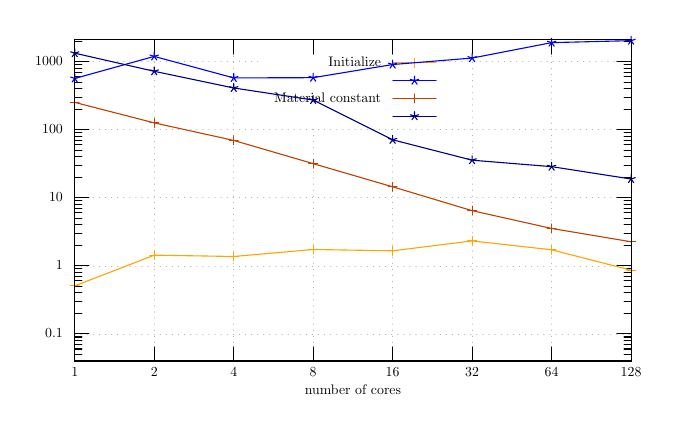
\begin{tikzpicture}[gnuplot]
%% generated with GNUPLOT 6.0p1 (Lua 5.4; terminal rev. Jun 2020, script rev. 118)
%% ven. 10 janv. 2025 17:58:53
\tikzset{every node/.append style={scale=0.50}}
\path (0.000,0.000) rectangle (8.125,4.725);
\gpcolor{color=gp lt color border}
\gpsetlinetype{gp lt border}
\gpsetdashtype{gp dt solid}
\gpsetlinewidth{1.00}
\draw[gp path] (0.598,0.492)--(0.688,0.492);
\draw[gp path] (7.664,0.492)--(7.574,0.492);
\draw[gp path] (0.598,0.576)--(0.688,0.576);
\draw[gp path] (7.664,0.576)--(7.574,0.576);
\draw[gp path] (0.598,0.644)--(0.688,0.644);
\draw[gp path] (7.664,0.644)--(7.574,0.644);
\draw[gp path] (0.598,0.702)--(0.688,0.702);
\draw[gp path] (7.664,0.702)--(7.574,0.702);
\draw[gp path] (0.598,0.752)--(0.688,0.752);
\draw[gp path] (7.664,0.752)--(7.574,0.752);
\draw[gp path] (0.598,0.796)--(0.688,0.796);
\draw[gp path] (7.664,0.796)--(7.574,0.796);
\gpcolor{color=gp lt color axes}
\gpsetlinetype{gp lt axes}
\gpsetdashtype{gp dt axes}
\gpsetlinewidth{0.50}
\draw[gp path] (0.598,0.836)--(7.664,0.836);
\gpcolor{color=gp lt color border}
\gpsetlinetype{gp lt border}
\gpsetdashtype{gp dt solid}
\gpsetlinewidth{1.00}
\draw[gp path] (0.598,0.836)--(0.778,0.836);
\draw[gp path] (7.664,0.836)--(7.484,0.836);
\node[gp node right] at (0.506,0.836) {$0.1$};
\draw[gp path] (0.598,1.096)--(0.688,1.096);
\draw[gp path] (7.664,1.096)--(7.574,1.096);
\draw[gp path] (0.598,1.248)--(0.688,1.248);
\draw[gp path] (7.664,1.248)--(7.574,1.248);
\draw[gp path] (0.598,1.356)--(0.688,1.356);
\draw[gp path] (7.664,1.356)--(7.574,1.356);
\draw[gp path] (0.598,1.440)--(0.688,1.440);
\draw[gp path] (7.664,1.440)--(7.574,1.440);
\draw[gp path] (0.598,1.509)--(0.688,1.509);
\draw[gp path] (7.664,1.509)--(7.574,1.509);
\draw[gp path] (0.598,1.566)--(0.688,1.566);
\draw[gp path] (7.664,1.566)--(7.574,1.566);
\draw[gp path] (0.598,1.617)--(0.688,1.617);
\draw[gp path] (7.664,1.617)--(7.574,1.617);
\draw[gp path] (0.598,1.661)--(0.688,1.661);
\draw[gp path] (7.664,1.661)--(7.574,1.661);
\gpcolor{color=gp lt color axes}
\gpsetlinetype{gp lt axes}
\gpsetdashtype{gp dt axes}
\gpsetlinewidth{0.50}
\draw[gp path] (0.598,1.700)--(7.664,1.700);
\gpcolor{color=gp lt color border}
\gpsetlinetype{gp lt border}
\gpsetdashtype{gp dt solid}
\gpsetlinewidth{1.00}
\draw[gp path] (0.598,1.700)--(0.778,1.700);
\draw[gp path] (7.664,1.700)--(7.484,1.700);
\node[gp node right] at (0.506,1.700) {$1$};
\draw[gp path] (0.598,1.960)--(0.688,1.960);
\draw[gp path] (7.664,1.960)--(7.574,1.960);
\draw[gp path] (0.598,2.113)--(0.688,2.113);
\draw[gp path] (7.664,2.113)--(7.574,2.113);
\draw[gp path] (0.598,2.221)--(0.688,2.221);
\draw[gp path] (7.664,2.221)--(7.574,2.221);
\draw[gp path] (0.598,2.304)--(0.688,2.304);
\draw[gp path] (7.664,2.304)--(7.574,2.304);
\draw[gp path] (0.598,2.373)--(0.688,2.373);
\draw[gp path] (7.664,2.373)--(7.574,2.373);
\draw[gp path] (0.598,2.431)--(0.688,2.431);
\draw[gp path] (7.664,2.431)--(7.574,2.431);
\draw[gp path] (0.598,2.481)--(0.688,2.481);
\draw[gp path] (7.664,2.481)--(7.574,2.481);
\draw[gp path] (0.598,2.525)--(0.688,2.525);
\draw[gp path] (7.664,2.525)--(7.574,2.525);
\gpcolor{color=gp lt color axes}
\gpsetlinetype{gp lt axes}
\gpsetdashtype{gp dt axes}
\gpsetlinewidth{0.50}
\draw[gp path] (0.598,2.565)--(7.664,2.565);
\gpcolor{color=gp lt color border}
\gpsetlinetype{gp lt border}
\gpsetdashtype{gp dt solid}
\gpsetlinewidth{1.00}
\draw[gp path] (0.598,2.565)--(0.778,2.565);
\draw[gp path] (7.664,2.565)--(7.484,2.565);
\node[gp node right] at (0.506,2.565) {$10$};
\draw[gp path] (0.598,2.825)--(0.688,2.825);
\draw[gp path] (7.664,2.825)--(7.574,2.825);
\draw[gp path] (0.598,2.977)--(0.688,2.977);
\draw[gp path] (7.664,2.977)--(7.574,2.977);
\draw[gp path] (0.598,3.085)--(0.688,3.085);
\draw[gp path] (7.664,3.085)--(7.574,3.085);
\draw[gp path] (0.598,3.169)--(0.688,3.169);
\draw[gp path] (7.664,3.169)--(7.574,3.169);
\draw[gp path] (0.598,3.237)--(0.688,3.237);
\draw[gp path] (7.664,3.237)--(7.574,3.237);
\draw[gp path] (0.598,3.295)--(0.688,3.295);
\draw[gp path] (7.664,3.295)--(7.574,3.295);
\draw[gp path] (0.598,3.345)--(0.688,3.345);
\draw[gp path] (7.664,3.345)--(7.574,3.345);
\draw[gp path] (0.598,3.389)--(0.688,3.389);
\draw[gp path] (7.664,3.389)--(7.574,3.389);
\gpcolor{color=gp lt color axes}
\gpsetlinetype{gp lt axes}
\gpsetdashtype{gp dt axes}
\gpsetlinewidth{0.50}
\draw[gp path] (0.598,3.429)--(7.664,3.429);
\gpcolor{color=gp lt color border}
\gpsetlinetype{gp lt border}
\gpsetdashtype{gp dt solid}
\gpsetlinewidth{1.00}
\draw[gp path] (0.598,3.429)--(0.778,3.429);
\draw[gp path] (7.664,3.429)--(7.484,3.429);
\node[gp node right] at (0.506,3.429) {$100$};
\draw[gp path] (0.598,3.689)--(0.688,3.689);
\draw[gp path] (7.664,3.689)--(7.574,3.689);
\draw[gp path] (0.598,3.841)--(0.688,3.841);
\draw[gp path] (7.664,3.841)--(7.574,3.841);
\draw[gp path] (0.598,3.949)--(0.688,3.949);
\draw[gp path] (7.664,3.949)--(7.574,3.949);
\draw[gp path] (0.598,4.033)--(0.688,4.033);
\draw[gp path] (7.664,4.033)--(7.574,4.033);
\draw[gp path] (0.598,4.102)--(0.688,4.102);
\draw[gp path] (7.664,4.102)--(7.574,4.102);
\draw[gp path] (0.598,4.159)--(0.688,4.159);
\draw[gp path] (7.664,4.159)--(7.574,4.159);
\draw[gp path] (0.598,4.210)--(0.688,4.210);
\draw[gp path] (7.664,4.210)--(7.574,4.210);
\draw[gp path] (0.598,4.254)--(0.688,4.254);
\draw[gp path] (7.664,4.254)--(7.574,4.254);
\gpcolor{color=gp lt color axes}
\gpsetlinetype{gp lt axes}
\gpsetdashtype{gp dt axes}
\gpsetlinewidth{0.50}
\draw[gp path] (0.598,4.293)--(2.983,4.293);
\draw[gp path] (5.279,4.293)--(7.664,4.293);
\gpcolor{color=gp lt color border}
\gpsetlinetype{gp lt border}
\gpsetdashtype{gp dt solid}
\gpsetlinewidth{1.00}
\draw[gp path] (0.598,4.293)--(0.778,4.293);
\draw[gp path] (7.664,4.293)--(7.484,4.293);
\node[gp node right] at (0.506,4.293) {$1000$};
\draw[gp path] (0.598,4.553)--(0.688,4.553);
\draw[gp path] (7.664,4.553)--(7.574,4.553);
\gpcolor{color=gp lt color axes}
\gpsetlinetype{gp lt axes}
\gpsetdashtype{gp dt axes}
\gpsetlinewidth{0.50}
\draw[gp path] (0.598,0.492)--(0.598,4.570);
\gpcolor{color=gp lt color border}
\gpsetlinetype{gp lt border}
\gpsetdashtype{gp dt solid}
\gpsetlinewidth{1.00}
\draw[gp path] (0.598,0.492)--(0.598,0.672);
\draw[gp path] (0.598,4.570)--(0.598,4.390);
\node[gp node center] at (0.598,0.338) {1};
\gpcolor{color=gp lt color axes}
\gpsetlinetype{gp lt axes}
\gpsetdashtype{gp dt axes}
\gpsetlinewidth{0.50}
\draw[gp path] (1.607,0.492)--(1.607,4.570);
\gpcolor{color=gp lt color border}
\gpsetlinetype{gp lt border}
\gpsetdashtype{gp dt solid}
\gpsetlinewidth{1.00}
\draw[gp path] (1.607,0.492)--(1.607,0.672);
\draw[gp path] (1.607,4.570)--(1.607,4.390);
\node[gp node center] at (1.607,0.338) {2};
\gpcolor{color=gp lt color axes}
\gpsetlinetype{gp lt axes}
\gpsetdashtype{gp dt axes}
\gpsetlinewidth{0.50}
\draw[gp path] (2.617,0.492)--(2.617,4.570);
\gpcolor{color=gp lt color border}
\gpsetlinetype{gp lt border}
\gpsetdashtype{gp dt solid}
\gpsetlinewidth{1.00}
\draw[gp path] (2.617,0.492)--(2.617,0.672);
\draw[gp path] (2.617,4.570)--(2.617,4.390);
\node[gp node center] at (2.617,0.338) {4};
\gpcolor{color=gp lt color axes}
\gpsetlinetype{gp lt axes}
\gpsetdashtype{gp dt axes}
\gpsetlinewidth{0.50}
\draw[gp path] (3.626,0.492)--(3.626,3.490);
\draw[gp path] (3.626,4.390)--(3.626,4.570);
\gpcolor{color=gp lt color border}
\gpsetlinetype{gp lt border}
\gpsetdashtype{gp dt solid}
\gpsetlinewidth{1.00}
\draw[gp path] (3.626,0.492)--(3.626,0.672);
\draw[gp path] (3.626,4.570)--(3.626,4.390);
\node[gp node center] at (3.626,0.338) {8};
\gpcolor{color=gp lt color axes}
\gpsetlinetype{gp lt axes}
\gpsetdashtype{gp dt axes}
\gpsetlinewidth{0.50}
\draw[gp path] (4.635,0.492)--(4.635,3.490);
\draw[gp path] (4.635,4.390)--(4.635,4.570);
\gpcolor{color=gp lt color border}
\gpsetlinetype{gp lt border}
\gpsetdashtype{gp dt solid}
\gpsetlinewidth{1.00}
\draw[gp path] (4.635,0.492)--(4.635,0.672);
\draw[gp path] (4.635,4.570)--(4.635,4.390);
\node[gp node center] at (4.635,0.338) {16};
\gpcolor{color=gp lt color axes}
\gpsetlinetype{gp lt axes}
\gpsetdashtype{gp dt axes}
\gpsetlinewidth{0.50}
\draw[gp path] (5.644,0.492)--(5.644,4.570);
\gpcolor{color=gp lt color border}
\gpsetlinetype{gp lt border}
\gpsetdashtype{gp dt solid}
\gpsetlinewidth{1.00}
\draw[gp path] (5.644,0.492)--(5.644,0.672);
\draw[gp path] (5.644,4.570)--(5.644,4.390);
\node[gp node center] at (5.644,0.338) {32};
\gpcolor{color=gp lt color axes}
\gpsetlinetype{gp lt axes}
\gpsetdashtype{gp dt axes}
\gpsetlinewidth{0.50}
\draw[gp path] (6.654,0.492)--(6.654,4.570);
\gpcolor{color=gp lt color border}
\gpsetlinetype{gp lt border}
\gpsetdashtype{gp dt solid}
\gpsetlinewidth{1.00}
\draw[gp path] (6.654,0.492)--(6.654,0.672);
\draw[gp path] (6.654,4.570)--(6.654,4.390);
\node[gp node center] at (6.654,0.338) {64};
\gpcolor{color=gp lt color axes}
\gpsetlinetype{gp lt axes}
\gpsetdashtype{gp dt axes}
\gpsetlinewidth{0.50}
\draw[gp path] (7.663,0.492)--(7.663,4.570);
\gpcolor{color=gp lt color border}
\gpsetlinetype{gp lt border}
\gpsetdashtype{gp dt solid}
\gpsetlinewidth{1.00}
\draw[gp path] (7.663,0.492)--(7.663,0.672);
\draw[gp path] (7.663,4.570)--(7.663,4.390);
\node[gp node center] at (7.663,0.338) {128};
\draw[gp path] (0.598,4.570)--(0.598,0.492)--(7.664,0.492)--(7.664,4.570)--cycle;
\node[gp node right] at (4.547,4.277) {Initialize};
\gpcolor{rgb color={1.000,0.647,0.000}}
\draw[gp path] (4.639,4.277)--(5.187,4.277);
\draw[gp path] (0.598,1.446)--(1.607,1.836)--(2.617,1.819)--(3.626,1.908)--(4.635,1.891)%
  --(5.644,2.017)--(6.654,1.904)--(7.663,1.645);
\gpsetpointsize{4.00}
\gp3point{gp mark 1}{}{(0.598,1.446)}
\gp3point{gp mark 1}{}{(1.607,1.836)}
\gp3point{gp mark 1}{}{(2.617,1.819)}
\gp3point{gp mark 1}{}{(3.626,1.908)}
\gp3point{gp mark 1}{}{(4.635,1.891)}
\gp3point{gp mark 1}{}{(5.644,2.017)}
\gp3point{gp mark 1}{}{(6.654,1.904)}
\gp3point{gp mark 1}{}{(7.663,1.645)}
\gp3point{gp mark 1}{}{(4.913,4.277)}
\gpcolor{color=gp lt color border}
\node[gp node right] at (4.547,4.052) { };
\gpcolor{rgb color={0.000,0.000,1.000}}
\draw[gp path] (4.639,4.052)--(5.187,4.052);
\draw[gp path] (0.598,4.080)--(1.607,4.360)--(2.617,4.087)--(3.626,4.090)--(4.635,4.257)%
  --(5.644,4.339)--(6.654,4.535)--(7.663,4.560);
\gp3point{gp mark 3}{}{(0.598,4.080)}
\gp3point{gp mark 3}{}{(1.607,4.360)}
\gp3point{gp mark 3}{}{(2.617,4.087)}
\gp3point{gp mark 3}{}{(3.626,4.090)}
\gp3point{gp mark 3}{}{(4.635,4.257)}
\gp3point{gp mark 3}{}{(5.644,4.339)}
\gp3point{gp mark 3}{}{(6.654,4.535)}
\gp3point{gp mark 3}{}{(7.663,4.560)}
\gp3point{gp mark 3}{}{(4.913,4.052)}
\gpcolor{color=gp lt color border}
\node[gp node right] at (4.547,3.827) {Material constant};
\gpcolor{rgb color={0.753,0.251,0.000}}
\draw[gp path] (4.639,3.827)--(5.187,3.827);
\draw[gp path] (0.598,3.776)--(1.607,3.516)--(2.617,3.293)--(3.626,2.998)--(4.635,2.704)%
  --(5.644,2.401)--(6.654,2.175)--(7.663,2.006);
\gp3point{gp mark 1}{}{(0.598,3.776)}
\gp3point{gp mark 1}{}{(1.607,3.516)}
\gp3point{gp mark 1}{}{(2.617,3.293)}
\gp3point{gp mark 1}{}{(3.626,2.998)}
\gp3point{gp mark 1}{}{(4.635,2.704)}
\gp3point{gp mark 1}{}{(5.644,2.401)}
\gp3point{gp mark 1}{}{(6.654,2.175)}
\gp3point{gp mark 1}{}{(7.663,2.006)}
\gp3point{gp mark 1}{}{(4.913,3.827)}
\gpcolor{color=gp lt color border}
\node[gp node right] at (4.547,3.602) { };
\gpcolor{rgb color={0.000,0.000,0.545}}
\draw[gp path] (4.639,3.602)--(5.187,3.602);
\draw[gp path] (0.598,4.401)--(1.607,4.171)--(2.617,3.959)--(3.626,3.806)--(4.635,3.301)%
  --(5.644,3.042)--(6.654,2.960)--(7.663,2.803);
\gp3point{gp mark 3}{}{(0.598,4.401)}
\gp3point{gp mark 3}{}{(1.607,4.171)}
\gp3point{gp mark 3}{}{(2.617,3.959)}
\gp3point{gp mark 3}{}{(3.626,3.806)}
\gp3point{gp mark 3}{}{(4.635,3.301)}
\gp3point{gp mark 3}{}{(5.644,3.042)}
\gp3point{gp mark 3}{}{(6.654,2.960)}
\gp3point{gp mark 3}{}{(7.663,2.803)}
\gp3point{gp mark 3}{}{(4.913,3.602)}
\gpcolor{color=gp lt color border}
\draw[gp path] (0.598,4.570)--(0.598,0.492)--(7.664,0.492)--(7.664,4.570)--cycle;
\node[gp node center] at (4.131,0.107) {number of cores};
%% coordinates of the plot area
\gpdefrectangularnode{gp plot 1}{\pgfpoint{0.598cm}{0.492cm}}{\pgfpoint{7.664cm}{4.570cm}}
\end{tikzpicture}
%% gnuplot variables
}\\
	\subfloat[Object creation (in s)]{
		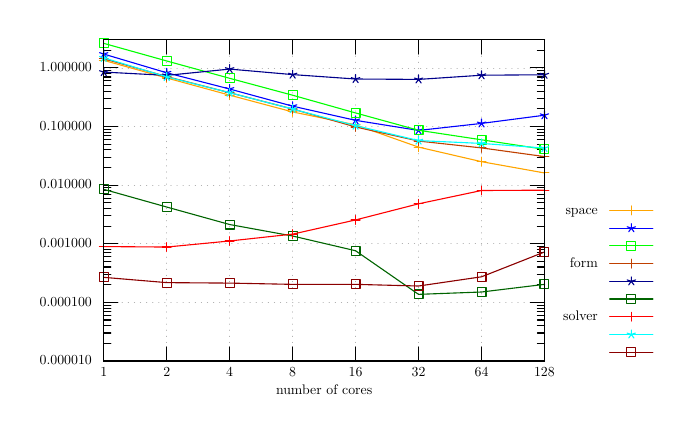
\begin{tikzpicture}[gnuplot]
%% generated with GNUPLOT 6.0p1 (Lua 5.4; terminal rev. Jun 2020, script rev. 118)
%% ven. 10 janv. 2025 17:58:53
\tikzset{every node/.append style={scale=0.50}}
\path (0.000,0.000) rectangle (8.125,4.725);
\gpcolor{color=gp lt color axes}
\gpsetlinetype{gp lt axes}
\gpsetdashtype{gp dt axes}
\gpsetlinewidth{0.50}
\draw[gp path] (0.966,0.492)--(6.564,0.492);
\gpcolor{color=gp lt color border}
\gpsetlinetype{gp lt border}
\gpsetdashtype{gp dt solid}
\gpsetlinewidth{1.00}
\draw[gp path] (0.966,0.492)--(1.146,0.492);
\draw[gp path] (6.564,0.492)--(6.384,0.492);
\node[gp node right] at (0.874,0.492) {0.000010};
\draw[gp path] (0.966,0.716)--(1.056,0.716);
\draw[gp path] (6.564,0.716)--(6.474,0.716);
\draw[gp path] (0.966,0.847)--(1.056,0.847);
\draw[gp path] (6.564,0.847)--(6.474,0.847);
\draw[gp path] (0.966,0.940)--(1.056,0.940);
\draw[gp path] (6.564,0.940)--(6.474,0.940);
\draw[gp path] (0.966,1.012)--(1.056,1.012);
\draw[gp path] (6.564,1.012)--(6.474,1.012);
\draw[gp path] (0.966,1.071)--(1.056,1.071);
\draw[gp path] (6.564,1.071)--(6.474,1.071);
\draw[gp path] (0.966,1.121)--(1.056,1.121);
\draw[gp path] (6.564,1.121)--(6.474,1.121);
\draw[gp path] (0.966,1.164)--(1.056,1.164);
\draw[gp path] (6.564,1.164)--(6.474,1.164);
\draw[gp path] (0.966,1.202)--(1.056,1.202);
\draw[gp path] (6.564,1.202)--(6.474,1.202);
\gpcolor{color=gp lt color axes}
\gpsetlinetype{gp lt axes}
\gpsetdashtype{gp dt axes}
\gpsetlinewidth{0.50}
\draw[gp path] (0.966,1.237)--(6.564,1.237);
\gpcolor{color=gp lt color border}
\gpsetlinetype{gp lt border}
\gpsetdashtype{gp dt solid}
\gpsetlinewidth{1.00}
\draw[gp path] (0.966,1.237)--(1.146,1.237);
\draw[gp path] (6.564,1.237)--(6.384,1.237);
\node[gp node right] at (0.874,1.237) {0.000100};
\draw[gp path] (0.966,1.461)--(1.056,1.461);
\draw[gp path] (6.564,1.461)--(6.474,1.461);
\draw[gp path] (0.966,1.592)--(1.056,1.592);
\draw[gp path] (6.564,1.592)--(6.474,1.592);
\draw[gp path] (0.966,1.685)--(1.056,1.685);
\draw[gp path] (6.564,1.685)--(6.474,1.685);
\draw[gp path] (0.966,1.757)--(1.056,1.757);
\draw[gp path] (6.564,1.757)--(6.474,1.757);
\draw[gp path] (0.966,1.816)--(1.056,1.816);
\draw[gp path] (6.564,1.816)--(6.474,1.816);
\draw[gp path] (0.966,1.866)--(1.056,1.866);
\draw[gp path] (6.564,1.866)--(6.474,1.866);
\draw[gp path] (0.966,1.909)--(1.056,1.909);
\draw[gp path] (6.564,1.909)--(6.474,1.909);
\draw[gp path] (0.966,1.947)--(1.056,1.947);
\draw[gp path] (6.564,1.947)--(6.474,1.947);
\gpcolor{color=gp lt color axes}
\gpsetlinetype{gp lt axes}
\gpsetdashtype{gp dt axes}
\gpsetlinewidth{0.50}
\draw[gp path] (0.966,1.981)--(6.564,1.981);
\gpcolor{color=gp lt color border}
\gpsetlinetype{gp lt border}
\gpsetdashtype{gp dt solid}
\gpsetlinewidth{1.00}
\draw[gp path] (0.966,1.981)--(1.146,1.981);
\draw[gp path] (6.564,1.981)--(6.384,1.981);
\node[gp node right] at (0.874,1.981) {0.001000};
\draw[gp path] (0.966,2.205)--(1.056,2.205);
\draw[gp path] (6.564,2.205)--(6.474,2.205);
\draw[gp path] (0.966,2.336)--(1.056,2.336);
\draw[gp path] (6.564,2.336)--(6.474,2.336);
\draw[gp path] (0.966,2.429)--(1.056,2.429);
\draw[gp path] (6.564,2.429)--(6.474,2.429);
\draw[gp path] (0.966,2.502)--(1.056,2.502);
\draw[gp path] (6.564,2.502)--(6.474,2.502);
\draw[gp path] (0.966,2.560)--(1.056,2.560);
\draw[gp path] (6.564,2.560)--(6.474,2.560);
\draw[gp path] (0.966,2.610)--(1.056,2.610);
\draw[gp path] (6.564,2.610)--(6.474,2.610);
\draw[gp path] (0.966,2.654)--(1.056,2.654);
\draw[gp path] (6.564,2.654)--(6.474,2.654);
\draw[gp path] (0.966,2.692)--(1.056,2.692);
\draw[gp path] (6.564,2.692)--(6.474,2.692);
\gpcolor{color=gp lt color axes}
\gpsetlinetype{gp lt axes}
\gpsetdashtype{gp dt axes}
\gpsetlinewidth{0.50}
\draw[gp path] (0.966,2.726)--(6.564,2.726);
\gpcolor{color=gp lt color border}
\gpsetlinetype{gp lt border}
\gpsetdashtype{gp dt solid}
\gpsetlinewidth{1.00}
\draw[gp path] (0.966,2.726)--(1.146,2.726);
\draw[gp path] (6.564,2.726)--(6.384,2.726);
\node[gp node right] at (0.874,2.726) {0.010000};
\draw[gp path] (0.966,2.950)--(1.056,2.950);
\draw[gp path] (6.564,2.950)--(6.474,2.950);
\draw[gp path] (0.966,3.081)--(1.056,3.081);
\draw[gp path] (6.564,3.081)--(6.474,3.081);
\draw[gp path] (0.966,3.174)--(1.056,3.174);
\draw[gp path] (6.564,3.174)--(6.474,3.174);
\draw[gp path] (0.966,3.246)--(1.056,3.246);
\draw[gp path] (6.564,3.246)--(6.474,3.246);
\draw[gp path] (0.966,3.305)--(1.056,3.305);
\draw[gp path] (6.564,3.305)--(6.474,3.305);
\draw[gp path] (0.966,3.355)--(1.056,3.355);
\draw[gp path] (6.564,3.355)--(6.474,3.355);
\draw[gp path] (0.966,3.398)--(1.056,3.398);
\draw[gp path] (6.564,3.398)--(6.474,3.398);
\draw[gp path] (0.966,3.436)--(1.056,3.436);
\draw[gp path] (6.564,3.436)--(6.474,3.436);
\gpcolor{color=gp lt color axes}
\gpsetlinetype{gp lt axes}
\gpsetdashtype{gp dt axes}
\gpsetlinewidth{0.50}
\draw[gp path] (0.966,3.470)--(6.564,3.470);
\gpcolor{color=gp lt color border}
\gpsetlinetype{gp lt border}
\gpsetdashtype{gp dt solid}
\gpsetlinewidth{1.00}
\draw[gp path] (0.966,3.470)--(1.146,3.470);
\draw[gp path] (6.564,3.470)--(6.384,3.470);
\node[gp node right] at (0.874,3.470) {0.100000};
\draw[gp path] (0.966,3.694)--(1.056,3.694);
\draw[gp path] (6.564,3.694)--(6.474,3.694);
\draw[gp path] (0.966,3.825)--(1.056,3.825);
\draw[gp path] (6.564,3.825)--(6.474,3.825);
\draw[gp path] (0.966,3.918)--(1.056,3.918);
\draw[gp path] (6.564,3.918)--(6.474,3.918);
\draw[gp path] (0.966,3.991)--(1.056,3.991);
\draw[gp path] (6.564,3.991)--(6.474,3.991);
\draw[gp path] (0.966,4.050)--(1.056,4.050);
\draw[gp path] (6.564,4.050)--(6.474,4.050);
\draw[gp path] (0.966,4.099)--(1.056,4.099);
\draw[gp path] (6.564,4.099)--(6.474,4.099);
\draw[gp path] (0.966,4.143)--(1.056,4.143);
\draw[gp path] (6.564,4.143)--(6.474,4.143);
\draw[gp path] (0.966,4.181)--(1.056,4.181);
\draw[gp path] (6.564,4.181)--(6.474,4.181);
\gpcolor{color=gp lt color axes}
\gpsetlinetype{gp lt axes}
\gpsetdashtype{gp dt axes}
\gpsetlinewidth{0.50}
\draw[gp path] (0.966,4.215)--(6.564,4.215);
\gpcolor{color=gp lt color border}
\gpsetlinetype{gp lt border}
\gpsetdashtype{gp dt solid}
\gpsetlinewidth{1.00}
\draw[gp path] (0.966,4.215)--(1.146,4.215);
\draw[gp path] (6.564,4.215)--(6.384,4.215);
\node[gp node right] at (0.874,4.215) {1.000000};
\draw[gp path] (0.966,4.439)--(1.056,4.439);
\draw[gp path] (6.564,4.439)--(6.474,4.439);
\draw[gp path] (0.966,4.570)--(1.056,4.570);
\draw[gp path] (6.564,4.570)--(6.474,4.570);
\gpcolor{color=gp lt color axes}
\gpsetlinetype{gp lt axes}
\gpsetdashtype{gp dt axes}
\gpsetlinewidth{0.50}
\draw[gp path] (0.966,0.492)--(0.966,4.570);
\gpcolor{color=gp lt color border}
\gpsetlinetype{gp lt border}
\gpsetdashtype{gp dt solid}
\gpsetlinewidth{1.00}
\draw[gp path] (0.966,0.492)--(0.966,0.672);
\draw[gp path] (0.966,4.570)--(0.966,4.390);
\node[gp node center] at (0.966,0.338) {1};
\gpcolor{color=gp lt color axes}
\gpsetlinetype{gp lt axes}
\gpsetdashtype{gp dt axes}
\gpsetlinewidth{0.50}
\draw[gp path] (1.766,0.492)--(1.766,4.570);
\gpcolor{color=gp lt color border}
\gpsetlinetype{gp lt border}
\gpsetdashtype{gp dt solid}
\gpsetlinewidth{1.00}
\draw[gp path] (1.766,0.492)--(1.766,0.672);
\draw[gp path] (1.766,4.570)--(1.766,4.390);
\node[gp node center] at (1.766,0.338) {2};
\gpcolor{color=gp lt color axes}
\gpsetlinetype{gp lt axes}
\gpsetdashtype{gp dt axes}
\gpsetlinewidth{0.50}
\draw[gp path] (2.565,0.492)--(2.565,4.570);
\gpcolor{color=gp lt color border}
\gpsetlinetype{gp lt border}
\gpsetdashtype{gp dt solid}
\gpsetlinewidth{1.00}
\draw[gp path] (2.565,0.492)--(2.565,0.672);
\draw[gp path] (2.565,4.570)--(2.565,4.390);
\node[gp node center] at (2.565,0.338) {4};
\gpcolor{color=gp lt color axes}
\gpsetlinetype{gp lt axes}
\gpsetdashtype{gp dt axes}
\gpsetlinewidth{0.50}
\draw[gp path] (3.365,0.492)--(3.365,4.570);
\gpcolor{color=gp lt color border}
\gpsetlinetype{gp lt border}
\gpsetdashtype{gp dt solid}
\gpsetlinewidth{1.00}
\draw[gp path] (3.365,0.492)--(3.365,0.672);
\draw[gp path] (3.365,4.570)--(3.365,4.390);
\node[gp node center] at (3.365,0.338) {8};
\gpcolor{color=gp lt color axes}
\gpsetlinetype{gp lt axes}
\gpsetdashtype{gp dt axes}
\gpsetlinewidth{0.50}
\draw[gp path] (4.164,0.492)--(4.164,4.570);
\gpcolor{color=gp lt color border}
\gpsetlinetype{gp lt border}
\gpsetdashtype{gp dt solid}
\gpsetlinewidth{1.00}
\draw[gp path] (4.164,0.492)--(4.164,0.672);
\draw[gp path] (4.164,4.570)--(4.164,4.390);
\node[gp node center] at (4.164,0.338) {16};
\gpcolor{color=gp lt color axes}
\gpsetlinetype{gp lt axes}
\gpsetdashtype{gp dt axes}
\gpsetlinewidth{0.50}
\draw[gp path] (4.964,0.492)--(4.964,4.570);
\gpcolor{color=gp lt color border}
\gpsetlinetype{gp lt border}
\gpsetdashtype{gp dt solid}
\gpsetlinewidth{1.00}
\draw[gp path] (4.964,0.492)--(4.964,0.672);
\draw[gp path] (4.964,4.570)--(4.964,4.390);
\node[gp node center] at (4.964,0.338) {32};
\gpcolor{color=gp lt color axes}
\gpsetlinetype{gp lt axes}
\gpsetdashtype{gp dt axes}
\gpsetlinewidth{0.50}
\draw[gp path] (5.764,0.492)--(5.764,4.570);
\gpcolor{color=gp lt color border}
\gpsetlinetype{gp lt border}
\gpsetdashtype{gp dt solid}
\gpsetlinewidth{1.00}
\draw[gp path] (5.764,0.492)--(5.764,0.672);
\draw[gp path] (5.764,4.570)--(5.764,4.390);
\node[gp node center] at (5.764,0.338) {64};
\gpcolor{color=gp lt color axes}
\gpsetlinetype{gp lt axes}
\gpsetdashtype{gp dt axes}
\gpsetlinewidth{0.50}
\draw[gp path] (6.563,0.492)--(6.563,4.570);
\gpcolor{color=gp lt color border}
\gpsetlinetype{gp lt border}
\gpsetdashtype{gp dt solid}
\gpsetlinewidth{1.00}
\draw[gp path] (6.563,0.492)--(6.563,0.672);
\draw[gp path] (6.563,4.570)--(6.563,4.390);
\node[gp node center] at (6.563,0.338) {128};
\draw[gp path] (0.966,4.570)--(0.966,0.492)--(6.564,0.492)--(6.564,4.570)--cycle;
\node[gp node right] at (7.300,2.404) {space};
\gpcolor{rgb color={1.000,0.647,0.000}}
\draw[gp path] (7.392,2.404)--(7.940,2.404);
\draw[gp path] (0.966,4.310)--(1.766,4.086)--(2.565,3.868)--(3.365,3.655)--(4.164,3.491)%
  --(4.964,3.208)--(5.764,3.023)--(6.563,2.880);
\gpsetpointsize{4.00}
\gp3point{gp mark 1}{}{(0.966,4.310)}
\gp3point{gp mark 1}{}{(1.766,4.086)}
\gp3point{gp mark 1}{}{(2.565,3.868)}
\gp3point{gp mark 1}{}{(3.365,3.655)}
\gp3point{gp mark 1}{}{(4.164,3.491)}
\gp3point{gp mark 1}{}{(4.964,3.208)}
\gp3point{gp mark 1}{}{(5.764,3.023)}
\gp3point{gp mark 1}{}{(6.563,2.880)}
\gp3point{gp mark 1}{}{(7.666,2.404)}
\gpcolor{color=gp lt color border}
\node[gp node right] at (7.300,2.179) { };
\gpcolor{rgb color={0.000,0.000,1.000}}
\draw[gp path] (7.392,2.179)--(7.940,2.179);
\draw[gp path] (0.966,4.390)--(1.766,4.152)--(2.565,3.946)--(3.365,3.728)--(4.164,3.548)%
  --(4.964,3.420)--(5.764,3.509)--(6.563,3.613);
\gp3point{gp mark 3}{}{(0.966,4.390)}
\gp3point{gp mark 3}{}{(1.766,4.152)}
\gp3point{gp mark 3}{}{(2.565,3.946)}
\gp3point{gp mark 3}{}{(3.365,3.728)}
\gp3point{gp mark 3}{}{(4.164,3.548)}
\gp3point{gp mark 3}{}{(4.964,3.420)}
\gp3point{gp mark 3}{}{(5.764,3.509)}
\gp3point{gp mark 3}{}{(6.563,3.613)}
\gp3point{gp mark 3}{}{(7.666,2.179)}
\gpcolor{color=gp lt color border}
\node[gp node right] at (7.300,1.954) { };
\gpcolor{rgb color={0.000,1.000,0.000}}
\draw[gp path] (7.392,1.954)--(7.940,1.954);
\draw[gp path] (0.966,4.526)--(1.766,4.302)--(2.565,4.082)--(3.365,3.867)--(4.164,3.642)%
  --(4.964,3.422)--(5.764,3.301)--(6.563,3.180);
\gp3point{gp mark 4}{}{(0.966,4.526)}
\gp3point{gp mark 4}{}{(1.766,4.302)}
\gp3point{gp mark 4}{}{(2.565,4.082)}
\gp3point{gp mark 4}{}{(3.365,3.867)}
\gp3point{gp mark 4}{}{(4.164,3.642)}
\gp3point{gp mark 4}{}{(4.964,3.422)}
\gp3point{gp mark 4}{}{(5.764,3.301)}
\gp3point{gp mark 4}{}{(6.563,3.180)}
\gp3point{gp mark 4}{}{(7.666,1.954)}
\gpcolor{color=gp lt color border}
\node[gp node right] at (7.300,1.729) {form};
\gpcolor{rgb color={0.753,0.251,0.000}}
\draw[gp path] (7.392,1.729)--(7.940,1.729);
\draw[gp path] (0.966,4.330)--(1.766,4.104)--(2.565,3.899)--(3.365,3.692)--(4.164,3.464)%
  --(4.964,3.285)--(5.764,3.198)--(6.563,3.088);
\gp3point{gp mark 1}{}{(0.966,4.330)}
\gp3point{gp mark 1}{}{(1.766,4.104)}
\gp3point{gp mark 1}{}{(2.565,3.899)}
\gp3point{gp mark 1}{}{(3.365,3.692)}
\gp3point{gp mark 1}{}{(4.164,3.464)}
\gp3point{gp mark 1}{}{(4.964,3.285)}
\gp3point{gp mark 1}{}{(5.764,3.198)}
\gp3point{gp mark 1}{}{(6.563,3.088)}
\gp3point{gp mark 1}{}{(7.666,1.729)}
\gpcolor{color=gp lt color border}
\node[gp node right] at (7.300,1.504) { };
\gpcolor{rgb color={0.000,0.000,0.545}}
\draw[gp path] (7.392,1.504)--(7.940,1.504);
\draw[gp path] (0.966,4.161)--(1.766,4.119)--(2.565,4.199)--(3.365,4.129)--(4.164,4.073)%
  --(4.964,4.068)--(5.764,4.121)--(6.563,4.127);
\gp3point{gp mark 3}{}{(0.966,4.161)}
\gp3point{gp mark 3}{}{(1.766,4.119)}
\gp3point{gp mark 3}{}{(2.565,4.199)}
\gp3point{gp mark 3}{}{(3.365,4.129)}
\gp3point{gp mark 3}{}{(4.164,4.073)}
\gp3point{gp mark 3}{}{(4.964,4.068)}
\gp3point{gp mark 3}{}{(5.764,4.121)}
\gp3point{gp mark 3}{}{(6.563,4.127)}
\gp3point{gp mark 3}{}{(7.666,1.504)}
\gpcolor{color=gp lt color border}
\node[gp node right] at (7.300,1.279) { };
\gpcolor{rgb color={0.000,0.392,0.000}}
\draw[gp path] (7.392,1.279)--(7.940,1.279);
\draw[gp path] (0.966,2.672)--(1.766,2.447)--(2.565,2.225)--(3.365,2.079)--(4.164,1.892)%
  --(4.964,1.338)--(5.764,1.368)--(6.563,1.465);
\gp3point{gp mark 4}{}{(0.966,2.672)}
\gp3point{gp mark 4}{}{(1.766,2.447)}
\gp3point{gp mark 4}{}{(2.565,2.225)}
\gp3point{gp mark 4}{}{(3.365,2.079)}
\gp3point{gp mark 4}{}{(4.164,1.892)}
\gp3point{gp mark 4}{}{(4.964,1.338)}
\gp3point{gp mark 4}{}{(5.764,1.368)}
\gp3point{gp mark 4}{}{(6.563,1.465)}
\gp3point{gp mark 4}{}{(7.666,1.279)}
\gpcolor{color=gp lt color border}
\node[gp node right] at (7.300,1.054) {solver};
\gpcolor{rgb color={1.000,0.000,0.000}}
\draw[gp path] (7.392,1.054)--(7.940,1.054);
\draw[gp path] (0.966,1.945)--(1.766,1.939)--(2.565,2.016)--(3.365,2.103)--(4.164,2.283)%
  --(4.964,2.488)--(5.764,2.657)--(6.563,2.661);
\gp3point{gp mark 1}{}{(0.966,1.945)}
\gp3point{gp mark 1}{}{(1.766,1.939)}
\gp3point{gp mark 1}{}{(2.565,2.016)}
\gp3point{gp mark 1}{}{(3.365,2.103)}
\gp3point{gp mark 1}{}{(4.164,2.283)}
\gp3point{gp mark 1}{}{(4.964,2.488)}
\gp3point{gp mark 1}{}{(5.764,2.657)}
\gp3point{gp mark 1}{}{(6.563,2.661)}
\gp3point{gp mark 1}{}{(7.666,1.054)}
\gpcolor{color=gp lt color border}
\node[gp node right] at (7.300,0.829) { };
\gpcolor{rgb color={0.000,1.000,1.000}}
\draw[gp path] (7.392,0.829)--(7.940,0.829);
\draw[gp path] (0.966,4.342)--(1.766,4.100)--(2.565,3.899)--(3.365,3.691)--(4.164,3.481)%
  --(4.964,3.291)--(5.764,3.255)--(6.563,3.196);
\gp3point{gp mark 3}{}{(0.966,4.342)}
\gp3point{gp mark 3}{}{(1.766,4.100)}
\gp3point{gp mark 3}{}{(2.565,3.899)}
\gp3point{gp mark 3}{}{(3.365,3.691)}
\gp3point{gp mark 3}{}{(4.164,3.481)}
\gp3point{gp mark 3}{}{(4.964,3.291)}
\gp3point{gp mark 3}{}{(5.764,3.255)}
\gp3point{gp mark 3}{}{(6.563,3.196)}
\gp3point{gp mark 3}{}{(7.666,0.829)}
\gpcolor{color=gp lt color border}
\node[gp node right] at (7.300,0.604) { };
\gpcolor{rgb color={0.545,0.000,0.000}}
\draw[gp path] (7.392,0.604)--(7.940,0.604);
\draw[gp path] (0.966,1.554)--(1.766,1.487)--(2.565,1.481)--(3.365,1.465)--(4.164,1.465)%
  --(4.964,1.444)--(5.764,1.561)--(6.563,1.876);
\gp3point{gp mark 4}{}{(0.966,1.554)}
\gp3point{gp mark 4}{}{(1.766,1.487)}
\gp3point{gp mark 4}{}{(2.565,1.481)}
\gp3point{gp mark 4}{}{(3.365,1.465)}
\gp3point{gp mark 4}{}{(4.164,1.465)}
\gp3point{gp mark 4}{}{(4.964,1.444)}
\gp3point{gp mark 4}{}{(5.764,1.561)}
\gp3point{gp mark 4}{}{(6.563,1.876)}
\gp3point{gp mark 4}{}{(7.666,0.604)}
\gpcolor{color=gp lt color border}
\draw[gp path] (0.966,4.570)--(0.966,0.492)--(6.564,0.492)--(6.564,4.570)--cycle;
\node[gp node center] at (3.765,0.107) {number of cores};
%% coordinates of the plot area
\gpdefrectangularnode{gp plot 1}{\pgfpoint{0.966cm}{0.492cm}}{\pgfpoint{6.564cm}{4.570cm}}
\end{tikzpicture}
%% gnuplot variables

	}
	\subfloat[Object creation (Ratio vs MFEM)]{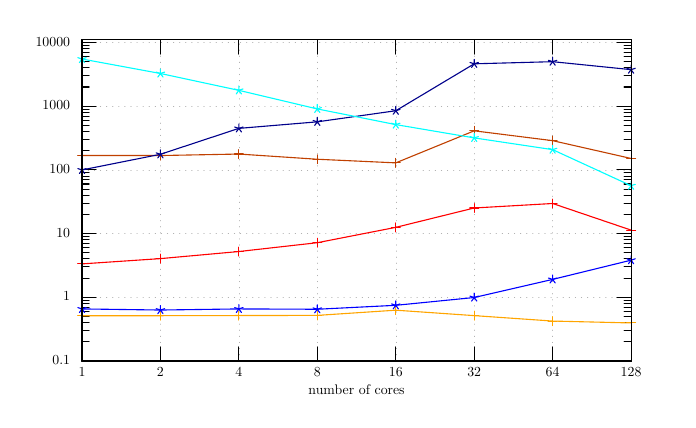
\begin{tikzpicture}[gnuplot]
%% generated with GNUPLOT 6.0p1 (Lua 5.4; terminal rev. Jun 2020, script rev. 118)
%% ven. 10 janv. 2025 17:58:53
\tikzset{every node/.append style={scale=0.50}}
\path (0.000,0.000) rectangle (8.125,4.725);
\gpcolor{color=gp lt color axes}
\gpsetlinetype{gp lt axes}
\gpsetdashtype{gp dt axes}
\gpsetlinewidth{0.50}
\draw[gp path] (0.690,0.492)--(7.664,0.492);
\gpcolor{color=gp lt color border}
\gpsetlinetype{gp lt border}
\gpsetdashtype{gp dt solid}
\gpsetlinewidth{1.00}
\draw[gp path] (0.690,0.492)--(0.870,0.492);
\draw[gp path] (7.664,0.492)--(7.484,0.492);
\node[gp node right] at (0.598,0.492) {$0.1$};
\draw[gp path] (0.690,0.736)--(0.780,0.736);
\draw[gp path] (7.664,0.736)--(7.574,0.736);
\draw[gp path] (0.690,0.878)--(0.780,0.878);
\draw[gp path] (7.664,0.878)--(7.574,0.878);
\draw[gp path] (0.690,0.979)--(0.780,0.979);
\draw[gp path] (7.664,0.979)--(7.574,0.979);
\draw[gp path] (0.690,1.057)--(0.780,1.057);
\draw[gp path] (7.664,1.057)--(7.574,1.057);
\draw[gp path] (0.690,1.121)--(0.780,1.121);
\draw[gp path] (7.664,1.121)--(7.574,1.121);
\draw[gp path] (0.690,1.176)--(0.780,1.176);
\draw[gp path] (7.664,1.176)--(7.574,1.176);
\draw[gp path] (0.690,1.223)--(0.780,1.223);
\draw[gp path] (7.664,1.223)--(7.574,1.223);
\draw[gp path] (0.690,1.264)--(0.780,1.264);
\draw[gp path] (7.664,1.264)--(7.574,1.264);
\gpcolor{color=gp lt color axes}
\gpsetlinetype{gp lt axes}
\gpsetdashtype{gp dt axes}
\gpsetlinewidth{0.50}
\draw[gp path] (0.690,1.301)--(7.664,1.301);
\gpcolor{color=gp lt color border}
\gpsetlinetype{gp lt border}
\gpsetdashtype{gp dt solid}
\gpsetlinewidth{1.00}
\draw[gp path] (0.690,1.301)--(0.870,1.301);
\draw[gp path] (7.664,1.301)--(7.484,1.301);
\node[gp node right] at (0.598,1.301) {$1$};
\draw[gp path] (0.690,1.544)--(0.780,1.544);
\draw[gp path] (7.664,1.544)--(7.574,1.544);
\draw[gp path] (0.690,1.687)--(0.780,1.687);
\draw[gp path] (7.664,1.687)--(7.574,1.687);
\draw[gp path] (0.690,1.788)--(0.780,1.788);
\draw[gp path] (7.664,1.788)--(7.574,1.788);
\draw[gp path] (0.690,1.866)--(0.780,1.866);
\draw[gp path] (7.664,1.866)--(7.574,1.866);
\draw[gp path] (0.690,1.930)--(0.780,1.930);
\draw[gp path] (7.664,1.930)--(7.574,1.930);
\draw[gp path] (0.690,1.985)--(0.780,1.985);
\draw[gp path] (7.664,1.985)--(7.574,1.985);
\draw[gp path] (0.690,2.031)--(0.780,2.031);
\draw[gp path] (7.664,2.031)--(7.574,2.031);
\draw[gp path] (0.690,2.073)--(0.780,2.073);
\draw[gp path] (7.664,2.073)--(7.574,2.073);
\gpcolor{color=gp lt color axes}
\gpsetlinetype{gp lt axes}
\gpsetdashtype{gp dt axes}
\gpsetlinewidth{0.50}
\draw[gp path] (0.690,2.110)--(7.664,2.110);
\gpcolor{color=gp lt color border}
\gpsetlinetype{gp lt border}
\gpsetdashtype{gp dt solid}
\gpsetlinewidth{1.00}
\draw[gp path] (0.690,2.110)--(0.870,2.110);
\draw[gp path] (7.664,2.110)--(7.484,2.110);
\node[gp node right] at (0.598,2.110) {$10$};
\draw[gp path] (0.690,2.353)--(0.780,2.353);
\draw[gp path] (7.664,2.353)--(7.574,2.353);
\draw[gp path] (0.690,2.496)--(0.780,2.496);
\draw[gp path] (7.664,2.496)--(7.574,2.496);
\draw[gp path] (0.690,2.597)--(0.780,2.597);
\draw[gp path] (7.664,2.597)--(7.574,2.597);
\draw[gp path] (0.690,2.675)--(0.780,2.675);
\draw[gp path] (7.664,2.675)--(7.574,2.675);
\draw[gp path] (0.690,2.739)--(0.780,2.739);
\draw[gp path] (7.664,2.739)--(7.574,2.739);
\draw[gp path] (0.690,2.793)--(0.780,2.793);
\draw[gp path] (7.664,2.793)--(7.574,2.793);
\draw[gp path] (0.690,2.840)--(0.780,2.840);
\draw[gp path] (7.664,2.840)--(7.574,2.840);
\draw[gp path] (0.690,2.882)--(0.780,2.882);
\draw[gp path] (7.664,2.882)--(7.574,2.882);
\gpcolor{color=gp lt color axes}
\gpsetlinetype{gp lt axes}
\gpsetdashtype{gp dt axes}
\gpsetlinewidth{0.50}
\draw[gp path] (0.690,2.919)--(7.664,2.919);
\gpcolor{color=gp lt color border}
\gpsetlinetype{gp lt border}
\gpsetdashtype{gp dt solid}
\gpsetlinewidth{1.00}
\draw[gp path] (0.690,2.919)--(0.870,2.919);
\draw[gp path] (7.664,2.919)--(7.484,2.919);
\node[gp node right] at (0.598,2.919) {$100$};
\draw[gp path] (0.690,3.162)--(0.780,3.162);
\draw[gp path] (7.664,3.162)--(7.574,3.162);
\draw[gp path] (0.690,3.305)--(0.780,3.305);
\draw[gp path] (7.664,3.305)--(7.574,3.305);
\draw[gp path] (0.690,3.406)--(0.780,3.406);
\draw[gp path] (7.664,3.406)--(7.574,3.406);
\draw[gp path] (0.690,3.484)--(0.780,3.484);
\draw[gp path] (7.664,3.484)--(7.574,3.484);
\draw[gp path] (0.690,3.548)--(0.780,3.548);
\draw[gp path] (7.664,3.548)--(7.574,3.548);
\draw[gp path] (0.690,3.602)--(0.780,3.602);
\draw[gp path] (7.664,3.602)--(7.574,3.602);
\draw[gp path] (0.690,3.649)--(0.780,3.649);
\draw[gp path] (7.664,3.649)--(7.574,3.649);
\draw[gp path] (0.690,3.691)--(0.780,3.691);
\draw[gp path] (7.664,3.691)--(7.574,3.691);
\gpcolor{color=gp lt color axes}
\gpsetlinetype{gp lt axes}
\gpsetdashtype{gp dt axes}
\gpsetlinewidth{0.50}
\draw[gp path] (0.690,3.728)--(7.664,3.728);
\gpcolor{color=gp lt color border}
\gpsetlinetype{gp lt border}
\gpsetdashtype{gp dt solid}
\gpsetlinewidth{1.00}
\draw[gp path] (0.690,3.728)--(0.870,3.728);
\draw[gp path] (7.664,3.728)--(7.484,3.728);
\node[gp node right] at (0.598,3.728) {$1000$};
\draw[gp path] (0.690,3.971)--(0.780,3.971);
\draw[gp path] (7.664,3.971)--(7.574,3.971);
\draw[gp path] (0.690,4.114)--(0.780,4.114);
\draw[gp path] (7.664,4.114)--(7.574,4.114);
\draw[gp path] (0.690,4.215)--(0.780,4.215);
\draw[gp path] (7.664,4.215)--(7.574,4.215);
\draw[gp path] (0.690,4.293)--(0.780,4.293);
\draw[gp path] (7.664,4.293)--(7.574,4.293);
\draw[gp path] (0.690,4.357)--(0.780,4.357);
\draw[gp path] (7.664,4.357)--(7.574,4.357);
\draw[gp path] (0.690,4.411)--(0.780,4.411);
\draw[gp path] (7.664,4.411)--(7.574,4.411);
\draw[gp path] (0.690,4.458)--(0.780,4.458);
\draw[gp path] (7.664,4.458)--(7.574,4.458);
\draw[gp path] (0.690,4.500)--(0.780,4.500);
\draw[gp path] (7.664,4.500)--(7.574,4.500);
\gpcolor{color=gp lt color axes}
\gpsetlinetype{gp lt axes}
\gpsetdashtype{gp dt axes}
\gpsetlinewidth{0.50}
\draw[gp path] (0.690,4.537)--(7.664,4.537);
\gpcolor{color=gp lt color border}
\gpsetlinetype{gp lt border}
\gpsetdashtype{gp dt solid}
\gpsetlinewidth{1.00}
\draw[gp path] (0.690,4.537)--(0.870,4.537);
\draw[gp path] (7.664,4.537)--(7.484,4.537);
\node[gp node right] at (0.598,4.537) {$10000$};
\gpcolor{color=gp lt color axes}
\gpsetlinetype{gp lt axes}
\gpsetdashtype{gp dt axes}
\gpsetlinewidth{0.50}
\draw[gp path] (0.690,0.492)--(0.690,4.570);
\gpcolor{color=gp lt color border}
\gpsetlinetype{gp lt border}
\gpsetdashtype{gp dt solid}
\gpsetlinewidth{1.00}
\draw[gp path] (0.690,0.492)--(0.690,0.672);
\draw[gp path] (0.690,4.570)--(0.690,4.390);
\node[gp node center] at (0.690,0.338) {1};
\gpcolor{color=gp lt color axes}
\gpsetlinetype{gp lt axes}
\gpsetdashtype{gp dt axes}
\gpsetlinewidth{0.50}
\draw[gp path] (1.686,0.492)--(1.686,4.570);
\gpcolor{color=gp lt color border}
\gpsetlinetype{gp lt border}
\gpsetdashtype{gp dt solid}
\gpsetlinewidth{1.00}
\draw[gp path] (1.686,0.492)--(1.686,0.672);
\draw[gp path] (1.686,4.570)--(1.686,4.390);
\node[gp node center] at (1.686,0.338) {2};
\gpcolor{color=gp lt color axes}
\gpsetlinetype{gp lt axes}
\gpsetdashtype{gp dt axes}
\gpsetlinewidth{0.50}
\draw[gp path] (2.682,0.492)--(2.682,4.570);
\gpcolor{color=gp lt color border}
\gpsetlinetype{gp lt border}
\gpsetdashtype{gp dt solid}
\gpsetlinewidth{1.00}
\draw[gp path] (2.682,0.492)--(2.682,0.672);
\draw[gp path] (2.682,4.570)--(2.682,4.390);
\node[gp node center] at (2.682,0.338) {4};
\gpcolor{color=gp lt color axes}
\gpsetlinetype{gp lt axes}
\gpsetdashtype{gp dt axes}
\gpsetlinewidth{0.50}
\draw[gp path] (3.678,0.492)--(3.678,4.570);
\gpcolor{color=gp lt color border}
\gpsetlinetype{gp lt border}
\gpsetdashtype{gp dt solid}
\gpsetlinewidth{1.00}
\draw[gp path] (3.678,0.492)--(3.678,0.672);
\draw[gp path] (3.678,4.570)--(3.678,4.390);
\node[gp node center] at (3.678,0.338) {8};
\gpcolor{color=gp lt color axes}
\gpsetlinetype{gp lt axes}
\gpsetdashtype{gp dt axes}
\gpsetlinewidth{0.50}
\draw[gp path] (4.675,0.492)--(4.675,4.570);
\gpcolor{color=gp lt color border}
\gpsetlinetype{gp lt border}
\gpsetdashtype{gp dt solid}
\gpsetlinewidth{1.00}
\draw[gp path] (4.675,0.492)--(4.675,0.672);
\draw[gp path] (4.675,4.570)--(4.675,4.390);
\node[gp node center] at (4.675,0.338) {16};
\gpcolor{color=gp lt color axes}
\gpsetlinetype{gp lt axes}
\gpsetdashtype{gp dt axes}
\gpsetlinewidth{0.50}
\draw[gp path] (5.671,0.492)--(5.671,4.570);
\gpcolor{color=gp lt color border}
\gpsetlinetype{gp lt border}
\gpsetdashtype{gp dt solid}
\gpsetlinewidth{1.00}
\draw[gp path] (5.671,0.492)--(5.671,0.672);
\draw[gp path] (5.671,4.570)--(5.671,4.390);
\node[gp node center] at (5.671,0.338) {32};
\gpcolor{color=gp lt color axes}
\gpsetlinetype{gp lt axes}
\gpsetdashtype{gp dt axes}
\gpsetlinewidth{0.50}
\draw[gp path] (6.667,0.492)--(6.667,4.570);
\gpcolor{color=gp lt color border}
\gpsetlinetype{gp lt border}
\gpsetdashtype{gp dt solid}
\gpsetlinewidth{1.00}
\draw[gp path] (6.667,0.492)--(6.667,0.672);
\draw[gp path] (6.667,4.570)--(6.667,4.390);
\node[gp node center] at (6.667,0.338) {64};
\gpcolor{color=gp lt color axes}
\gpsetlinetype{gp lt axes}
\gpsetdashtype{gp dt axes}
\gpsetlinewidth{0.50}
\draw[gp path] (7.663,0.492)--(7.663,4.570);
\gpcolor{color=gp lt color border}
\gpsetlinetype{gp lt border}
\gpsetdashtype{gp dt solid}
\gpsetlinewidth{1.00}
\draw[gp path] (7.663,0.492)--(7.663,0.672);
\draw[gp path] (7.663,4.570)--(7.663,4.390);
\node[gp node center] at (7.663,0.338) {128};
\draw[gp path] (0.690,4.570)--(0.690,0.492)--(7.664,0.492)--(7.664,4.570)--cycle;
\gpcolor{rgb color={1.000,0.647,0.000}}
\draw[gp path] (0.690,1.067)--(1.686,1.067)--(2.682,1.069)--(3.678,1.071)--(4.675,1.137)%
  --(5.671,1.068)--(6.667,0.999)--(7.663,0.975);
\gpsetpointsize{4.00}
\gp3point{gp mark 1}{}{(0.690,1.067)}
\gp3point{gp mark 1}{}{(1.686,1.067)}
\gp3point{gp mark 1}{}{(2.682,1.069)}
\gp3point{gp mark 1}{}{(3.678,1.071)}
\gp3point{gp mark 1}{}{(4.675,1.137)}
\gp3point{gp mark 1}{}{(5.671,1.068)}
\gp3point{gp mark 1}{}{(6.667,0.999)}
\gp3point{gp mark 1}{}{(7.663,0.975)}
\gpcolor{rgb color={0.000,0.000,1.000}}
\draw[gp path] (0.690,1.153)--(1.686,1.139)--(2.682,1.153)--(3.678,1.149)--(4.675,1.199)%
  --(5.671,1.298)--(6.667,1.528)--(7.663,1.772);
\gp3point{gp mark 3}{}{(0.690,1.153)}
\gp3point{gp mark 3}{}{(1.686,1.139)}
\gp3point{gp mark 3}{}{(2.682,1.153)}
\gp3point{gp mark 3}{}{(3.678,1.149)}
\gp3point{gp mark 3}{}{(4.675,1.199)}
\gp3point{gp mark 3}{}{(5.671,1.298)}
\gp3point{gp mark 3}{}{(6.667,1.528)}
\gp3point{gp mark 3}{}{(7.663,1.772)}
\gpcolor{rgb color={0.753,0.251,0.000}}
\draw[gp path] (0.690,3.101)--(1.686,3.101)--(2.682,3.120)--(3.678,3.054)--(4.675,3.008)%
  --(5.671,3.415)--(6.667,3.290)--(7.663,3.064);
\gp3point{gp mark 1}{}{(0.690,3.101)}
\gp3point{gp mark 1}{}{(1.686,3.101)}
\gp3point{gp mark 1}{}{(2.682,3.120)}
\gp3point{gp mark 1}{}{(3.678,3.054)}
\gp3point{gp mark 1}{}{(4.675,3.008)}
\gp3point{gp mark 1}{}{(5.671,3.415)}
\gp3point{gp mark 1}{}{(6.667,3.290)}
\gp3point{gp mark 1}{}{(7.663,3.064)}
\gpcolor{rgb color={0.000,0.000,0.545}}
\draw[gp path] (0.690,2.918)--(1.686,3.117)--(2.682,3.446)--(3.678,3.529)--(4.675,3.670)%
  --(5.671,4.266)--(6.667,4.293)--(7.663,4.192);
\gp3point{gp mark 3}{}{(0.690,2.918)}
\gp3point{gp mark 3}{}{(1.686,3.117)}
\gp3point{gp mark 3}{}{(2.682,3.446)}
\gp3point{gp mark 3}{}{(3.678,3.529)}
\gp3point{gp mark 3}{}{(4.675,3.670)}
\gp3point{gp mark 3}{}{(5.671,4.266)}
\gp3point{gp mark 3}{}{(6.667,4.293)}
\gp3point{gp mark 3}{}{(7.663,4.192)}
\gpcolor{rgb color={1.000,0.000,0.000}}
\draw[gp path] (0.690,1.725)--(1.686,1.792)--(2.682,1.882)--(3.678,1.994)--(4.675,2.189)%
  --(5.671,2.435)--(6.667,2.492)--(7.663,2.154);
\gp3point{gp mark 1}{}{(0.690,1.725)}
\gp3point{gp mark 1}{}{(1.686,1.792)}
\gp3point{gp mark 1}{}{(2.682,1.882)}
\gp3point{gp mark 1}{}{(3.678,1.994)}
\gp3point{gp mark 1}{}{(4.675,2.189)}
\gp3point{gp mark 1}{}{(5.671,2.435)}
\gp3point{gp mark 1}{}{(6.667,2.492)}
\gp3point{gp mark 1}{}{(7.663,2.154)}
\gpcolor{rgb color={0.000,1.000,1.000}}
\draw[gp path] (0.690,4.327)--(1.686,4.143)--(2.682,3.929)--(3.678,3.693)--(4.675,3.494)%
  --(5.671,3.325)--(6.667,3.176)--(7.663,2.718);
\gp3point{gp mark 3}{}{(0.690,4.327)}
\gp3point{gp mark 3}{}{(1.686,4.143)}
\gp3point{gp mark 3}{}{(2.682,3.929)}
\gp3point{gp mark 3}{}{(3.678,3.693)}
\gp3point{gp mark 3}{}{(4.675,3.494)}
\gp3point{gp mark 3}{}{(5.671,3.325)}
\gp3point{gp mark 3}{}{(6.667,3.176)}
\gp3point{gp mark 3}{}{(7.663,2.718)}
\gpcolor{color=gp lt color border}
\draw[gp path] (0.690,4.570)--(0.690,0.492)--(7.664,0.492)--(7.664,4.570)--cycle;
\node[gp node center] at (4.177,0.107) {number of cores};
%% coordinates of the plot area
\gpdefrectangularnode{gp plot 1}{\pgfpoint{0.690cm}{0.492cm}}{\pgfpoint{7.664cm}{4.570cm}}
\end{tikzpicture}
%% gnuplot variables
}\\
	\subfloat[Boundary condition (in s)]{
		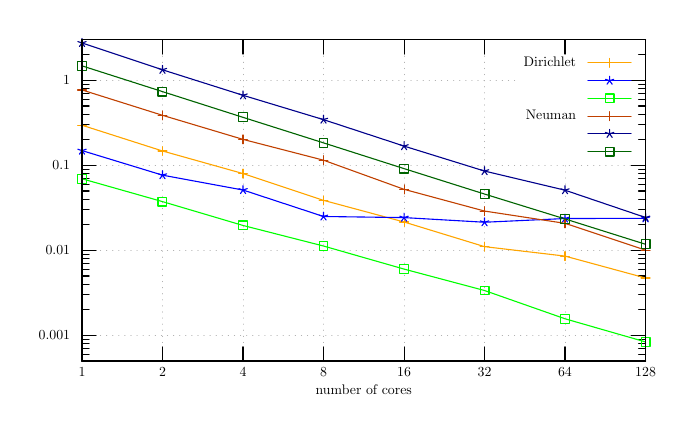
\begin{tikzpicture}[gnuplot]
%% generated with GNUPLOT 6.0p1 (Lua 5.4; terminal rev. Jun 2020, script rev. 118)
%% ven. 10 janv. 2025 17:58:53
\tikzset{every node/.append style={scale=0.50}}
\path (0.000,0.000) rectangle (8.125,4.725);
\gpcolor{color=gp lt color border}
\gpsetlinetype{gp lt border}
\gpsetdashtype{gp dt solid}
\gpsetlinewidth{1.00}
\draw[gp path] (0.690,0.492)--(0.780,0.492);
\draw[gp path] (7.848,0.492)--(7.758,0.492);
\draw[gp path] (0.690,0.577)--(0.780,0.577);
\draw[gp path] (7.848,0.577)--(7.758,0.577);
\draw[gp path] (0.690,0.650)--(0.780,0.650);
\draw[gp path] (7.848,0.650)--(7.758,0.650);
\draw[gp path] (0.690,0.712)--(0.780,0.712);
\draw[gp path] (7.848,0.712)--(7.758,0.712);
\draw[gp path] (0.690,0.768)--(0.780,0.768);
\draw[gp path] (7.848,0.768)--(7.758,0.768);
\gpcolor{color=gp lt color axes}
\gpsetlinetype{gp lt axes}
\gpsetdashtype{gp dt axes}
\gpsetlinewidth{0.50}
\draw[gp path] (0.690,0.817)--(7.848,0.817);
\gpcolor{color=gp lt color border}
\gpsetlinetype{gp lt border}
\gpsetdashtype{gp dt solid}
\gpsetlinewidth{1.00}
\draw[gp path] (0.690,0.817)--(0.870,0.817);
\draw[gp path] (7.848,0.817)--(7.668,0.817);
\node[gp node right] at (0.598,0.817) {$0.001$};
\draw[gp path] (0.690,1.142)--(0.780,1.142);
\draw[gp path] (7.848,1.142)--(7.758,1.142);
\draw[gp path] (0.690,1.332)--(0.780,1.332);
\draw[gp path] (7.848,1.332)--(7.758,1.332);
\draw[gp path] (0.690,1.467)--(0.780,1.467);
\draw[gp path] (7.848,1.467)--(7.758,1.467);
\draw[gp path] (0.690,1.571)--(0.780,1.571);
\draw[gp path] (7.848,1.571)--(7.758,1.571);
\draw[gp path] (0.690,1.657)--(0.780,1.657);
\draw[gp path] (7.848,1.657)--(7.758,1.657);
\draw[gp path] (0.690,1.729)--(0.780,1.729);
\draw[gp path] (7.848,1.729)--(7.758,1.729);
\draw[gp path] (0.690,1.792)--(0.780,1.792);
\draw[gp path] (7.848,1.792)--(7.758,1.792);
\draw[gp path] (0.690,1.847)--(0.780,1.847);
\draw[gp path] (7.848,1.847)--(7.758,1.847);
\gpcolor{color=gp lt color axes}
\gpsetlinetype{gp lt axes}
\gpsetdashtype{gp dt axes}
\gpsetlinewidth{0.50}
\draw[gp path] (0.690,1.896)--(7.848,1.896);
\gpcolor{color=gp lt color border}
\gpsetlinetype{gp lt border}
\gpsetdashtype{gp dt solid}
\gpsetlinewidth{1.00}
\draw[gp path] (0.690,1.896)--(0.870,1.896);
\draw[gp path] (7.848,1.896)--(7.668,1.896);
\node[gp node right] at (0.598,1.896) {$0.01$};
\draw[gp path] (0.690,2.221)--(0.780,2.221);
\draw[gp path] (7.848,2.221)--(7.758,2.221);
\draw[gp path] (0.690,2.411)--(0.780,2.411);
\draw[gp path] (7.848,2.411)--(7.758,2.411);
\draw[gp path] (0.690,2.546)--(0.780,2.546);
\draw[gp path] (7.848,2.546)--(7.758,2.546);
\draw[gp path] (0.690,2.651)--(0.780,2.651);
\draw[gp path] (7.848,2.651)--(7.758,2.651);
\draw[gp path] (0.690,2.736)--(0.780,2.736);
\draw[gp path] (7.848,2.736)--(7.758,2.736);
\draw[gp path] (0.690,2.808)--(0.780,2.808);
\draw[gp path] (7.848,2.808)--(7.758,2.808);
\draw[gp path] (0.690,2.871)--(0.780,2.871);
\draw[gp path] (7.848,2.871)--(7.758,2.871);
\draw[gp path] (0.690,2.926)--(0.780,2.926);
\draw[gp path] (7.848,2.926)--(7.758,2.926);
\gpcolor{color=gp lt color axes}
\gpsetlinetype{gp lt axes}
\gpsetdashtype{gp dt axes}
\gpsetlinewidth{0.50}
\draw[gp path] (0.690,2.976)--(7.848,2.976);
\gpcolor{color=gp lt color border}
\gpsetlinetype{gp lt border}
\gpsetdashtype{gp dt solid}
\gpsetlinewidth{1.00}
\draw[gp path] (0.690,2.976)--(0.870,2.976);
\draw[gp path] (7.848,2.976)--(7.668,2.976);
\node[gp node right] at (0.598,2.976) {$0.1$};
\draw[gp path] (0.690,3.301)--(0.780,3.301);
\draw[gp path] (7.848,3.301)--(7.758,3.301);
\draw[gp path] (0.690,3.491)--(0.780,3.491);
\draw[gp path] (7.848,3.491)--(7.758,3.491);
\draw[gp path] (0.690,3.625)--(0.780,3.625);
\draw[gp path] (7.848,3.625)--(7.758,3.625);
\draw[gp path] (0.690,3.730)--(0.780,3.730);
\draw[gp path] (7.848,3.730)--(7.758,3.730);
\draw[gp path] (0.690,3.816)--(0.780,3.816);
\draw[gp path] (7.848,3.816)--(7.758,3.816);
\draw[gp path] (0.690,3.888)--(0.780,3.888);
\draw[gp path] (7.848,3.888)--(7.758,3.888);
\draw[gp path] (0.690,3.950)--(0.780,3.950);
\draw[gp path] (7.848,3.950)--(7.758,3.950);
\draw[gp path] (0.690,4.006)--(0.780,4.006);
\draw[gp path] (7.848,4.006)--(7.758,4.006);
\gpcolor{color=gp lt color axes}
\gpsetlinetype{gp lt axes}
\gpsetdashtype{gp dt axes}
\gpsetlinewidth{0.50}
\draw[gp path] (0.690,4.055)--(6.196,4.055);
\draw[gp path] (7.756,4.055)--(7.848,4.055);
\gpcolor{color=gp lt color border}
\gpsetlinetype{gp lt border}
\gpsetdashtype{gp dt solid}
\gpsetlinewidth{1.00}
\draw[gp path] (0.690,4.055)--(0.870,4.055);
\draw[gp path] (7.848,4.055)--(7.668,4.055);
\node[gp node right] at (0.598,4.055) {$1$};
\draw[gp path] (0.690,4.380)--(0.780,4.380);
\draw[gp path] (7.848,4.380)--(7.758,4.380);
\draw[gp path] (0.690,4.570)--(0.780,4.570);
\draw[gp path] (7.848,4.570)--(7.758,4.570);
\gpcolor{color=gp lt color axes}
\gpsetlinetype{gp lt axes}
\gpsetdashtype{gp dt axes}
\gpsetlinewidth{0.50}
\draw[gp path] (0.690,0.492)--(0.690,4.570);
\gpcolor{color=gp lt color border}
\gpsetlinetype{gp lt border}
\gpsetdashtype{gp dt solid}
\gpsetlinewidth{1.00}
\draw[gp path] (0.690,0.492)--(0.690,0.672);
\draw[gp path] (0.690,4.570)--(0.690,4.390);
\node[gp node center] at (0.690,0.338) {1};
\gpcolor{color=gp lt color axes}
\gpsetlinetype{gp lt axes}
\gpsetdashtype{gp dt axes}
\gpsetlinewidth{0.50}
\draw[gp path] (1.712,0.492)--(1.712,4.570);
\gpcolor{color=gp lt color border}
\gpsetlinetype{gp lt border}
\gpsetdashtype{gp dt solid}
\gpsetlinewidth{1.00}
\draw[gp path] (1.712,0.492)--(1.712,0.672);
\draw[gp path] (1.712,4.570)--(1.712,4.390);
\node[gp node center] at (1.712,0.338) {2};
\gpcolor{color=gp lt color axes}
\gpsetlinetype{gp lt axes}
\gpsetdashtype{gp dt axes}
\gpsetlinewidth{0.50}
\draw[gp path] (2.735,0.492)--(2.735,4.570);
\gpcolor{color=gp lt color border}
\gpsetlinetype{gp lt border}
\gpsetdashtype{gp dt solid}
\gpsetlinewidth{1.00}
\draw[gp path] (2.735,0.492)--(2.735,0.672);
\draw[gp path] (2.735,4.570)--(2.735,4.390);
\node[gp node center] at (2.735,0.338) {4};
\gpcolor{color=gp lt color axes}
\gpsetlinetype{gp lt axes}
\gpsetdashtype{gp dt axes}
\gpsetlinewidth{0.50}
\draw[gp path] (3.757,0.492)--(3.757,4.570);
\gpcolor{color=gp lt color border}
\gpsetlinetype{gp lt border}
\gpsetdashtype{gp dt solid}
\gpsetlinewidth{1.00}
\draw[gp path] (3.757,0.492)--(3.757,0.672);
\draw[gp path] (3.757,4.570)--(3.757,4.390);
\node[gp node center] at (3.757,0.338) {8};
\gpcolor{color=gp lt color axes}
\gpsetlinetype{gp lt axes}
\gpsetdashtype{gp dt axes}
\gpsetlinewidth{0.50}
\draw[gp path] (4.780,0.492)--(4.780,4.570);
\gpcolor{color=gp lt color border}
\gpsetlinetype{gp lt border}
\gpsetdashtype{gp dt solid}
\gpsetlinewidth{1.00}
\draw[gp path] (4.780,0.492)--(4.780,0.672);
\draw[gp path] (4.780,4.570)--(4.780,4.390);
\node[gp node center] at (4.780,0.338) {16};
\gpcolor{color=gp lt color axes}
\gpsetlinetype{gp lt axes}
\gpsetdashtype{gp dt axes}
\gpsetlinewidth{0.50}
\draw[gp path] (5.802,0.492)--(5.802,4.570);
\gpcolor{color=gp lt color border}
\gpsetlinetype{gp lt border}
\gpsetdashtype{gp dt solid}
\gpsetlinewidth{1.00}
\draw[gp path] (5.802,0.492)--(5.802,0.672);
\draw[gp path] (5.802,4.570)--(5.802,4.390);
\node[gp node center] at (5.802,0.338) {32};
\gpcolor{color=gp lt color axes}
\gpsetlinetype{gp lt axes}
\gpsetdashtype{gp dt axes}
\gpsetlinewidth{0.50}
\draw[gp path] (6.824,0.492)--(6.824,3.040);
\draw[gp path] (6.824,4.390)--(6.824,4.570);
\gpcolor{color=gp lt color border}
\gpsetlinetype{gp lt border}
\gpsetdashtype{gp dt solid}
\gpsetlinewidth{1.00}
\draw[gp path] (6.824,0.492)--(6.824,0.672);
\draw[gp path] (6.824,4.570)--(6.824,4.390);
\node[gp node center] at (6.824,0.338) {64};
\gpcolor{color=gp lt color axes}
\gpsetlinetype{gp lt axes}
\gpsetdashtype{gp dt axes}
\gpsetlinewidth{0.50}
\draw[gp path] (7.847,0.492)--(7.847,4.570);
\gpcolor{color=gp lt color border}
\gpsetlinetype{gp lt border}
\gpsetdashtype{gp dt solid}
\gpsetlinewidth{1.00}
\draw[gp path] (7.847,0.492)--(7.847,0.672);
\draw[gp path] (7.847,4.570)--(7.847,4.390);
\node[gp node center] at (7.847,0.338) {128};
\draw[gp path] (0.690,4.570)--(0.690,0.492)--(7.848,0.492)--(7.848,4.570)--cycle;
\node[gp node right] at (7.024,4.277) {Dirichlet};
\gpcolor{rgb color={1.000,0.647,0.000}}
\draw[gp path] (7.116,4.277)--(7.664,4.277);
\draw[gp path] (0.690,3.486)--(1.712,3.159)--(2.735,2.872)--(3.757,2.532)--(4.780,2.257)%
  --(5.802,1.944)--(6.824,1.824)--(7.847,1.546);
\gpsetpointsize{4.00}
\gp3point{gp mark 1}{}{(0.690,3.486)}
\gp3point{gp mark 1}{}{(1.712,3.159)}
\gp3point{gp mark 1}{}{(2.735,2.872)}
\gp3point{gp mark 1}{}{(3.757,2.532)}
\gp3point{gp mark 1}{}{(4.780,2.257)}
\gp3point{gp mark 1}{}{(5.802,1.944)}
\gp3point{gp mark 1}{}{(6.824,1.824)}
\gp3point{gp mark 1}{}{(7.847,1.546)}
\gp3point{gp mark 1}{}{(7.390,4.277)}
\gpcolor{color=gp lt color border}
\node[gp node right] at (7.024,4.052) { };
\gpcolor{rgb color={0.000,0.000,1.000}}
\draw[gp path] (7.116,4.052)--(7.664,4.052);
\draw[gp path] (0.690,3.164)--(1.712,2.852)--(2.735,2.663)--(3.757,2.327)--(4.780,2.313)%
  --(5.802,2.254)--(6.824,2.301)--(7.847,2.304);
\gp3point{gp mark 3}{}{(0.690,3.164)}
\gp3point{gp mark 3}{}{(1.712,2.852)}
\gp3point{gp mark 3}{}{(2.735,2.663)}
\gp3point{gp mark 3}{}{(3.757,2.327)}
\gp3point{gp mark 3}{}{(4.780,2.313)}
\gp3point{gp mark 3}{}{(5.802,2.254)}
\gp3point{gp mark 3}{}{(6.824,2.301)}
\gp3point{gp mark 3}{}{(7.847,2.304)}
\gp3point{gp mark 3}{}{(7.390,4.052)}
\gpcolor{color=gp lt color border}
\node[gp node right] at (7.024,3.827) { };
\gpcolor{rgb color={0.000,1.000,0.000}}
\draw[gp path] (7.116,3.827)--(7.664,3.827);
\draw[gp path] (0.690,2.806)--(1.712,2.516)--(2.735,2.213)--(3.757,1.952)--(4.780,1.659)%
  --(5.802,1.387)--(6.824,1.028)--(7.847,0.734);
\gp3point{gp mark 4}{}{(0.690,2.806)}
\gp3point{gp mark 4}{}{(1.712,2.516)}
\gp3point{gp mark 4}{}{(2.735,2.213)}
\gp3point{gp mark 4}{}{(3.757,1.952)}
\gp3point{gp mark 4}{}{(4.780,1.659)}
\gp3point{gp mark 4}{}{(5.802,1.387)}
\gp3point{gp mark 4}{}{(6.824,1.028)}
\gp3point{gp mark 4}{}{(7.847,0.734)}
\gp3point{gp mark 4}{}{(7.390,3.827)}
\gpcolor{color=gp lt color border}
\node[gp node right] at (7.024,3.602) {Neuman};
\gpcolor{rgb color={0.753,0.251,0.000}}
\draw[gp path] (7.116,3.602)--(7.664,3.602);
\draw[gp path] (0.690,3.934)--(1.712,3.612)--(2.735,3.306)--(3.757,3.042)--(4.780,2.672)%
  --(5.802,2.396)--(6.824,2.240)--(7.847,1.900);
\gp3point{gp mark 1}{}{(0.690,3.934)}
\gp3point{gp mark 1}{}{(1.712,3.612)}
\gp3point{gp mark 1}{}{(2.735,3.306)}
\gp3point{gp mark 1}{}{(3.757,3.042)}
\gp3point{gp mark 1}{}{(4.780,2.672)}
\gp3point{gp mark 1}{}{(5.802,2.396)}
\gp3point{gp mark 1}{}{(6.824,2.240)}
\gp3point{gp mark 1}{}{(7.847,1.900)}
\gp3point{gp mark 1}{}{(7.390,3.602)}
\gpcolor{color=gp lt color border}
\node[gp node right] at (7.024,3.377) { };
\gpcolor{rgb color={0.000,0.000,0.545}}
\draw[gp path] (7.116,3.377)--(7.664,3.377);
\draw[gp path] (0.690,4.531)--(1.712,4.190)--(2.735,3.866)--(3.757,3.557)--(4.780,3.221)%
  --(5.802,2.904)--(6.824,2.661)--(7.847,2.314);
\gp3point{gp mark 3}{}{(0.690,4.531)}
\gp3point{gp mark 3}{}{(1.712,4.190)}
\gp3point{gp mark 3}{}{(2.735,3.866)}
\gp3point{gp mark 3}{}{(3.757,3.557)}
\gp3point{gp mark 3}{}{(4.780,3.221)}
\gp3point{gp mark 3}{}{(5.802,2.904)}
\gp3point{gp mark 3}{}{(6.824,2.661)}
\gp3point{gp mark 3}{}{(7.847,2.314)}
\gp3point{gp mark 3}{}{(7.390,3.377)}
\gpcolor{color=gp lt color border}
\node[gp node right] at (7.024,3.152) { };
\gpcolor{rgb color={0.000,0.392,0.000}}
\draw[gp path] (7.116,3.152)--(7.664,3.152);
\draw[gp path] (0.690,4.240)--(1.712,3.913)--(2.735,3.586)--(3.757,3.262)--(4.780,2.935)%
  --(5.802,2.612)--(6.824,2.296)--(7.847,1.974);
\gp3point{gp mark 4}{}{(0.690,4.240)}
\gp3point{gp mark 4}{}{(1.712,3.913)}
\gp3point{gp mark 4}{}{(2.735,3.586)}
\gp3point{gp mark 4}{}{(3.757,3.262)}
\gp3point{gp mark 4}{}{(4.780,2.935)}
\gp3point{gp mark 4}{}{(5.802,2.612)}
\gp3point{gp mark 4}{}{(6.824,2.296)}
\gp3point{gp mark 4}{}{(7.847,1.974)}
\gp3point{gp mark 4}{}{(7.390,3.152)}
\gpcolor{color=gp lt color border}
\draw[gp path] (0.690,4.570)--(0.690,0.492)--(7.848,0.492)--(7.848,4.570)--cycle;
\node[gp node center] at (4.269,0.107) {number of cores};
%% coordinates of the plot area
\gpdefrectangularnode{gp plot 1}{\pgfpoint{0.690cm}{0.492cm}}{\pgfpoint{7.848cm}{4.570cm}}
\end{tikzpicture}
%% gnuplot variables

	}
	\subfloat[Boundary condition (Ratio vs MFEM)]{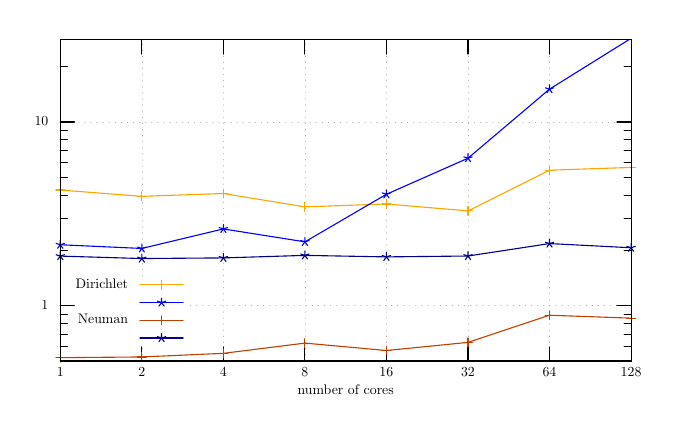
\begin{tikzpicture}[gnuplot]
%% generated with GNUPLOT 6.0p1 (Lua 5.4; terminal rev. Jun 2020, script rev. 118)
%% ven. 10 janv. 2025 17:58:53
\tikzset{every node/.append style={scale=0.50}}
\path (0.000,0.000) rectangle (8.125,4.725);
\gpcolor{color=gp lt color border}
\gpsetlinetype{gp lt border}
\gpsetdashtype{gp dt solid}
\gpsetlinewidth{1.00}
\draw[gp path] (0.414,0.492)--(0.504,0.492);
\draw[gp path] (7.664,0.492)--(7.574,0.492);
\draw[gp path] (0.414,0.677)--(0.504,0.677);
\draw[gp path] (7.664,0.677)--(7.574,0.677);
\draw[gp path] (0.414,0.833)--(0.504,0.833);
\draw[gp path] (7.664,0.833)--(7.574,0.833);
\draw[gp path] (0.414,0.968)--(0.504,0.968);
\draw[gp path] (7.664,0.968)--(7.574,0.968);
\draw[gp path] (0.414,1.087)--(0.504,1.087);
\draw[gp path] (7.664,1.087)--(7.574,1.087);
\gpcolor{color=gp lt color axes}
\gpsetlinetype{gp lt axes}
\gpsetdashtype{gp dt axes}
\gpsetlinewidth{0.50}
\draw[gp path] (0.414,1.194)--(0.506,1.194);
\draw[gp path] (2.066,1.194)--(7.664,1.194);
\gpcolor{color=gp lt color border}
\gpsetlinetype{gp lt border}
\gpsetdashtype{gp dt solid}
\gpsetlinewidth{1.00}
\draw[gp path] (0.414,1.194)--(0.594,1.194);
\draw[gp path] (7.664,1.194)--(7.484,1.194);
\node[gp node right] at (0.322,1.194) {$1$};
\draw[gp path] (0.414,1.896)--(0.504,1.896);
\draw[gp path] (7.664,1.896)--(7.574,1.896);
\draw[gp path] (0.414,2.307)--(0.504,2.307);
\draw[gp path] (7.664,2.307)--(7.574,2.307);
\draw[gp path] (0.414,2.599)--(0.504,2.599);
\draw[gp path] (7.664,2.599)--(7.574,2.599);
\draw[gp path] (0.414,2.825)--(0.504,2.825);
\draw[gp path] (7.664,2.825)--(7.574,2.825);
\draw[gp path] (0.414,3.009)--(0.504,3.009);
\draw[gp path] (7.664,3.009)--(7.574,3.009);
\draw[gp path] (0.414,3.166)--(0.504,3.166);
\draw[gp path] (7.664,3.166)--(7.574,3.166);
\draw[gp path] (0.414,3.301)--(0.504,3.301);
\draw[gp path] (7.664,3.301)--(7.574,3.301);
\draw[gp path] (0.414,3.420)--(0.504,3.420);
\draw[gp path] (7.664,3.420)--(7.574,3.420);
\gpcolor{color=gp lt color axes}
\gpsetlinetype{gp lt axes}
\gpsetdashtype{gp dt axes}
\gpsetlinewidth{0.50}
\draw[gp path] (0.414,3.527)--(7.664,3.527);
\gpcolor{color=gp lt color border}
\gpsetlinetype{gp lt border}
\gpsetdashtype{gp dt solid}
\gpsetlinewidth{1.00}
\draw[gp path] (0.414,3.527)--(0.594,3.527);
\draw[gp path] (7.664,3.527)--(7.484,3.527);
\node[gp node right] at (0.322,3.527) {$10$};
\draw[gp path] (0.414,4.229)--(0.504,4.229);
\draw[gp path] (7.664,4.229)--(7.574,4.229);
\gpcolor{color=gp lt color axes}
\gpsetlinetype{gp lt axes}
\gpsetdashtype{gp dt axes}
\gpsetlinewidth{0.50}
\draw[gp path] (0.414,0.492)--(0.414,4.570);
\gpcolor{color=gp lt color border}
\gpsetlinetype{gp lt border}
\gpsetdashtype{gp dt solid}
\gpsetlinewidth{1.00}
\draw[gp path] (0.414,0.492)--(0.414,0.672);
\draw[gp path] (0.414,4.570)--(0.414,4.390);
\node[gp node center] at (0.414,0.338) {1};
\gpcolor{color=gp lt color axes}
\gpsetlinetype{gp lt axes}
\gpsetdashtype{gp dt axes}
\gpsetlinewidth{0.50}
\draw[gp path] (1.450,0.492)--(1.450,0.672);
\draw[gp path] (1.450,1.572)--(1.450,4.570);
\gpcolor{color=gp lt color border}
\gpsetlinetype{gp lt border}
\gpsetdashtype{gp dt solid}
\gpsetlinewidth{1.00}
\draw[gp path] (1.450,0.492)--(1.450,0.672);
\draw[gp path] (1.450,4.570)--(1.450,4.390);
\node[gp node center] at (1.450,0.338) {2};
\gpcolor{color=gp lt color axes}
\gpsetlinetype{gp lt axes}
\gpsetdashtype{gp dt axes}
\gpsetlinewidth{0.50}
\draw[gp path] (2.485,0.492)--(2.485,4.570);
\gpcolor{color=gp lt color border}
\gpsetlinetype{gp lt border}
\gpsetdashtype{gp dt solid}
\gpsetlinewidth{1.00}
\draw[gp path] (2.485,0.492)--(2.485,0.672);
\draw[gp path] (2.485,4.570)--(2.485,4.390);
\node[gp node center] at (2.485,0.338) {4};
\gpcolor{color=gp lt color axes}
\gpsetlinetype{gp lt axes}
\gpsetdashtype{gp dt axes}
\gpsetlinewidth{0.50}
\draw[gp path] (3.521,0.492)--(3.521,4.570);
\gpcolor{color=gp lt color border}
\gpsetlinetype{gp lt border}
\gpsetdashtype{gp dt solid}
\gpsetlinewidth{1.00}
\draw[gp path] (3.521,0.492)--(3.521,0.672);
\draw[gp path] (3.521,4.570)--(3.521,4.390);
\node[gp node center] at (3.521,0.338) {8};
\gpcolor{color=gp lt color axes}
\gpsetlinetype{gp lt axes}
\gpsetdashtype{gp dt axes}
\gpsetlinewidth{0.50}
\draw[gp path] (4.556,0.492)--(4.556,4.570);
\gpcolor{color=gp lt color border}
\gpsetlinetype{gp lt border}
\gpsetdashtype{gp dt solid}
\gpsetlinewidth{1.00}
\draw[gp path] (4.556,0.492)--(4.556,0.672);
\draw[gp path] (4.556,4.570)--(4.556,4.390);
\node[gp node center] at (4.556,0.338) {16};
\gpcolor{color=gp lt color axes}
\gpsetlinetype{gp lt axes}
\gpsetdashtype{gp dt axes}
\gpsetlinewidth{0.50}
\draw[gp path] (5.592,0.492)--(5.592,4.570);
\gpcolor{color=gp lt color border}
\gpsetlinetype{gp lt border}
\gpsetdashtype{gp dt solid}
\gpsetlinewidth{1.00}
\draw[gp path] (5.592,0.492)--(5.592,0.672);
\draw[gp path] (5.592,4.570)--(5.592,4.390);
\node[gp node center] at (5.592,0.338) {32};
\gpcolor{color=gp lt color axes}
\gpsetlinetype{gp lt axes}
\gpsetdashtype{gp dt axes}
\gpsetlinewidth{0.50}
\draw[gp path] (6.627,0.492)--(6.627,4.570);
\gpcolor{color=gp lt color border}
\gpsetlinetype{gp lt border}
\gpsetdashtype{gp dt solid}
\gpsetlinewidth{1.00}
\draw[gp path] (6.627,0.492)--(6.627,0.672);
\draw[gp path] (6.627,4.570)--(6.627,4.390);
\node[gp node center] at (6.627,0.338) {64};
\gpcolor{color=gp lt color axes}
\gpsetlinetype{gp lt axes}
\gpsetdashtype{gp dt axes}
\gpsetlinewidth{0.50}
\draw[gp path] (7.663,0.492)--(7.663,4.570);
\gpcolor{color=gp lt color border}
\gpsetlinetype{gp lt border}
\gpsetdashtype{gp dt solid}
\gpsetlinewidth{1.00}
\draw[gp path] (7.663,0.492)--(7.663,0.672);
\draw[gp path] (7.663,4.570)--(7.663,4.390);
\node[gp node center] at (7.663,0.338) {128};
\draw[gp path] (0.414,4.570)--(0.414,0.492)--(7.664,0.492)--(7.664,4.570)--cycle;
\node[gp node right] at (1.334,1.459) {Dirichlet};
\gpcolor{rgb color={1.000,0.647,0.000}}
\draw[gp path] (1.426,1.459)--(1.974,1.459);
\draw[gp path] (0.414,2.663)--(1.450,2.583)--(2.485,2.619)--(3.521,2.449)--(4.556,2.486)%
  --(5.592,2.398)--(6.627,2.915)--(7.663,2.950);
\gpsetpointsize{4.00}
\gp3point{gp mark 1}{}{(0.414,2.663)}
\gp3point{gp mark 1}{}{(1.450,2.583)}
\gp3point{gp mark 1}{}{(2.485,2.619)}
\gp3point{gp mark 1}{}{(3.521,2.449)}
\gp3point{gp mark 1}{}{(4.556,2.486)}
\gp3point{gp mark 1}{}{(5.592,2.398)}
\gp3point{gp mark 1}{}{(6.627,2.915)}
\gp3point{gp mark 1}{}{(7.663,2.950)}
\gp3point{gp mark 1}{}{(1.700,1.459)}
\gpcolor{color=gp lt color border}
\node[gp node right] at (1.334,1.234) { };
\gpcolor{rgb color={0.000,0.000,1.000}}
\draw[gp path] (1.426,1.234)--(1.974,1.234);
\draw[gp path] (0.414,1.968)--(1.450,1.921)--(2.485,2.169)--(3.521,2.005)--(4.556,2.609)%
  --(5.592,3.067)--(6.627,3.944)--(7.632,4.570);
\gp3point{gp mark 3}{}{(0.414,1.968)}
\gp3point{gp mark 3}{}{(1.450,1.921)}
\gp3point{gp mark 3}{}{(2.485,2.169)}
\gp3point{gp mark 3}{}{(3.521,2.005)}
\gp3point{gp mark 3}{}{(4.556,2.609)}
\gp3point{gp mark 3}{}{(5.592,3.067)}
\gp3point{gp mark 3}{}{(6.627,3.944)}
\gp3point{gp mark 3}{}{(1.700,1.234)}
\gpcolor{color=gp lt color border}
\node[gp node right] at (1.334,1.009) {Neuman};
\gpcolor{rgb color={0.753,0.251,0.000}}
\draw[gp path] (1.426,1.009)--(1.974,1.009);
\draw[gp path] (0.414,0.534)--(1.450,0.543)--(2.485,0.589)--(3.521,0.719)--(4.556,0.625)%
  --(5.592,0.728)--(6.627,1.073)--(7.663,1.036);
\gp3point{gp mark 1}{}{(0.414,0.534)}
\gp3point{gp mark 1}{}{(1.450,0.543)}
\gp3point{gp mark 1}{}{(2.485,0.589)}
\gp3point{gp mark 1}{}{(3.521,0.719)}
\gp3point{gp mark 1}{}{(4.556,0.625)}
\gp3point{gp mark 1}{}{(5.592,0.728)}
\gp3point{gp mark 1}{}{(6.627,1.073)}
\gp3point{gp mark 1}{}{(7.663,1.036)}
\gp3point{gp mark 1}{}{(1.700,1.009)}
\gpcolor{color=gp lt color border}
\node[gp node right] at (1.334,0.784) { };
\gpcolor{rgb color={0.000,0.000,0.545}}
\draw[gp path] (1.426,0.784)--(1.974,0.784);
\draw[gp path] (0.414,1.824)--(1.450,1.793)--(2.485,1.801)--(3.521,1.833)--(4.556,1.814)%
  --(5.592,1.825)--(6.627,1.983)--(7.663,1.930);
\gp3point{gp mark 3}{}{(0.414,1.824)}
\gp3point{gp mark 3}{}{(1.450,1.793)}
\gp3point{gp mark 3}{}{(2.485,1.801)}
\gp3point{gp mark 3}{}{(3.521,1.833)}
\gp3point{gp mark 3}{}{(4.556,1.814)}
\gp3point{gp mark 3}{}{(5.592,1.825)}
\gp3point{gp mark 3}{}{(6.627,1.983)}
\gp3point{gp mark 3}{}{(7.663,1.930)}
\gp3point{gp mark 3}{}{(1.700,0.784)}
\gpcolor{color=gp lt color border}
\draw[gp path] (0.414,4.570)--(0.414,0.492)--(7.664,0.492)--(7.664,4.570)--cycle;
\node[gp node center] at (4.039,0.107) {number of cores};
%% coordinates of the plot area
\gpdefrectangularnode{gp plot 1}{\pgfpoint{0.414cm}{0.492cm}}{\pgfpoint{7.664cm}{4.570cm}}
\end{tikzpicture}
%% gnuplot variables
}\\
	\caption{Elapsed time function of the number of processes: miscellaneous initiation, major object creation and Boundary conditions (in log-log scale except for y axes of \protect\subref*{time_nl_r} )\label{elapsed5}}
\end{figure}
\clearpage
\end{document}
This is never printed


